%% LyX 2.4.3 created this file.  For more info, see https://www.lyx.org/.
%% Do not edit unless you really know what you are doing.
\documentclass[oneside,american,english]{book}
\usepackage[T1]{fontenc}
\usepackage[latin9]{inputenc}
\setcounter{secnumdepth}{3}
\setcounter{tocdepth}{1}
\usepackage{array}
\usepackage{float}
\usepackage{multirow}
\usepackage{amsmath}
\usepackage{amsthm}
\usepackage{amssymb}
\usepackage{graphicx}
\usepackage{rotating}

\makeatletter

%%%%%%%%%%%%%%%%%%%%%%%%%%%%%% LyX specific LaTeX commands.
%% Because html converters don't know tabularnewline
\providecommand{\tabularnewline}{\\}
%% A simple dot to overcome graphicx limitations
\newcommand{\lyxdot}{.}


%%%%%%%%%%%%%%%%%%%%%%%%%%%%%% Textclass specific LaTeX commands.
\input{preamble.tex}

%%%%%%%%%%%%%%%%%%%%%%%%%%%%%% User specified LaTeX commands.
\usepackage{url}
\usepackage{xargs}
\usepackage{amsfonts}
\usepackage{amssymb}
%\usepackage[pdftex,dvipsnames]{xcolor}
\usepackage{float}
\usepackage[colorinlistoftodos,prependcaption,textsize=tiny]{todonotes}
\usepackage[lined,boxed,ruled,norelsize,algo2e]{algorithm2e}
\usepackage[small,bf]{caption}
\usepackage{tikz}
\usepackage{enumitem}
\usepackage[stable]{footmisc}
\setlist{nolistsep}
\usepackage{hyperref}
\hypersetup{
    colorlinks,
    citecolor=red,
    filecolor=red,
    linkcolor=red,
    urlcolor=red
}

\makeatother

\usepackage{babel}
\begin{document}
\global\long\def\R{\mathbb{R}}%
\global\long\def\RR{\mathbb{{\cal R}}}%
\global\long\def\Rn{\mathbb{R}^{n}}%
\global\long\def\Rm{\mathbb{R}^{m}}%
\global\long\def\norm#1{\left\Vert #1\right\Vert }%
\global\long\def\defeq{\overset{\mathrm{def}}{=}}%
\global\long\def\dom{\mathrm{dom}}%
\global\long\def\vol{\mathrm{vol}}%
\global\long\def\nnz{\mathrm{nnz}}%
\global\long\def\E{\mathbf{E}}%
\global\long\def\P{\mathbf{P}}%
\global\long\def\tr{\mathrm{tr}}%
\global\long\def\op{\mathrm{op}}%
\global\long\def\argmin{\mathrm{argmin}}%
\global\long\def\argmax{\mathrm{argmax}}%
\global\long\def\epi{\mathrm{epi}}%
\global\long\def\KL{d_{\mathrm{KL}}}%
\global\long\def\last{(\mathrm{last})}%
\global\long\def\new{(\mathrm{new})}%
\global\long\def\ls{\mathtt{lineSearch}}%
\global\long\def\conv{\mathrm{conv}}%
\global\long\def\Lip{\mathrm{Lip}}%
\global\long\def\Diag{\mathrm{Diag}}%
\global\long\def\step{\delta}%
\global\long\def\spn{\mathrm{span}}%
\global\long\def\K{\mathcal{K}}%
\global\long\def\d{\mathcal{\mathrm{d}}}%
\global\long\def\T{\mathcal{\mathcal{T}}}%
\global\long\def\diag{\mathrm{diag}}%
\global\long\def\one{\mathbb{{\bf 1}}}%
\global\long\def\abs#1{\left\vert #1\right\vert }%
\global\long\def\bdiag{\mathbf{Diag}}%
\global\long\def\mh{\mathbf{H}}%
\global\long\def\mi{\mathbf{I}}%
\global\long\def\mv{\mathbf{V}}%
\global\long\def\mw{\mathbf{W}}%
\global\long\def\ms{\mathbf{S}}%
\global\long\def\mproj{\mathbf{P}}%
\global\long\def\msigma{\mathbf{\Sigma}}%
\global\long\def\ma{\mathbf{A}}%
\global\long\def\poly{\mbox{poly}}%
\global\long\def\cov{\mathrm{Cov}}%
\global\long\def\oma{\overline{\ma}}%
\global\long\def\Var{\mathrm{Var}}%
\global\long\def\rank{\mathrm{rank}}%
\global\long\def\Ent{\mathrm{Ent}}%
\global\long\def\spe{\mathrm{op}}%
\global\long\def\esssup{\operatorname{ess\,sup}}%
\global\long\def\tv{\mathrm{TV}}%
\global\long\def\PriR{\mathcal{P}}%
 
\global\long\def\DualR{\mathcal{D}}%
 
\title{Techniques in Optimization and Sampling\\
(book in progress with improving citations)}
\author{Yin Tat Lee\thanks{yintat@uw.edu. This work is supported in part by CCF-1749609, DMS-1839116,
DMS-2023166, Microsoft Research Faculty Fellowship, Sloan Research
Fellowship and Packard Fellowships.}\\
\\
University of Washington\\
\& OpenAI \and  Santosh S. Vempala\thanks{vempala@gatech.edu. This work is supported in part by CCF-1563838,
E2CDA-1640081, CCF-1717349 and DMS-1839323.}\\
\\
Georgia Tech}

\maketitle
\tableofcontents{}

\newpage{}

\chapter*{Preliminaries}


\section*{Notation}

We use $B(x,r)$ to denote the Euclidean (or $\ell_{2}$) ball centered
at $x$ with radius $r$: $\left\{ y:\norm{y-x}_{2}\le r\right\} $.
We use $\conv(X)$ to denote the convex hull of $X$, namely $\conv(X)=\{\sum\alpha_{i}x_{i}:\ \alpha_{i}\geq0,\sum\alpha_{i}=1,x_{i}\in X\}$.
We use $\left\langle x,y\right\rangle $ to denote the $\ell_{2}$
inner product $x^{T}y$ of $x$ and $y$. For any two points $x,y\in\Rn$,
we view them as column vectors, and use $[x,y]$ to denote $\conv(\{x,y\})$,
namely, the line segment between $x$ and $y$. 

We use $e_{i}$ to denote the coordinate vector whose $i$-th coordinate
is 1 and all other coordinates are $0$.


\section*{Functions}
\begin{defn}
For any $L\geq0$, a function $f:V\rightarrow W$ is $L$-Lipschitz
if $\norm{f(x)-f(y)}_{W}\leq L\norm{x-y}_{V}$ where the norms $\norm{\cdot}_{V}$
and $\norm{\cdot}_{W}$ are $\ell_{2}$ norms if unspecified.
\end{defn}

\begin{defn}
A function $f\in\mathcal{C}^{k}(\Rn)$ if $f$ is a $k$-differentiable
function and its $k^{\mathrm{th}}$ derivative is continuous.
\end{defn}

\begin{defn}
\label{def:lower-semi}A function ${\displaystyle f:X\subseteq\R^{n}\to\R}$
is called lower semi-continuous at a point $x_{0}\in X$ if for every
real $y<f(x_{0})$ there exists a neighborhood $U$ of $x_{0}$ such
that $f(x)>y$ for all $x\in U$. Equivalently, $f$ is lower semi-continuous
at $x_{0}$ iff 

\[
{\displaystyle \liminf_{x\to x_{0}}f(x)\geq f(x_{0})}.
\]
The function is lower semi-continuous if is it so at every point in
its domain. The definition of upper semi-continuous is analogous with
the inequalities reversed and $\liminf$ replaced by $\limsup$. 
\end{defn}

\begin{thm}[Taylor's Remainder Theorem]
\label{thm:taylor_expansion}For any $g\in\mathcal{C}^{k+1}(\R)$,
and any $x$ and $y$, there is a $\zeta\in[x,y]$ such that
\[
g(y)=\sum_{j=0}^{k}g^{(j)}(x)\frac{(y-x)^{j}}{j!}+g^{(k+1)}(\zeta)\frac{(y-x)^{k+1}}{(k+1)!}.
\]
\end{thm}

\begin{defn}
The $convolution$ of two functions $f,g:\R^{n}\rightarrow\R$ is
defined as $h(x)=\int_{\R^{n}}f(z)g(x-z)\,dz.$
\end{defn}


\section*{Linear Algebra}
\begin{defn}
\label{def:PSD}A real symmetric matrix $A$ is positive semi-definite
(PSD) if $x^{\top}Ax\geq0$ for all $x\in\Rn$. Equivalently, a real
symmetric matrix with all nonnegative eigenvalues is PSD. We write
$A\succeq0$ if $A$ is PSD and $A\succeq B$ if $A-B$ is PSD.
\end{defn}

\begin{defn}
For any matrix $A$, we define its trace, $\tr A=\sum A_{ii}$, Frobenius
norm, $\,\|A\|_{F}^{2}=\tr(A^{\top}A)=\sum_{i,j}A_{ij}^{2}$, and
operator norm, $\,\|A\|_{\op}=\sup_{\|x\|_{2}=1}\|Ax\|_{2}$. Note
that $x^{\top}Ax=\tr(Axx^{\top})$ and in general, $\tr(AB)=\tr(BA)$.
\end{defn}

For symmetric $A$, we have $\tr A=\sum_{i}\lambda_{i}$, $\|A\|_{F}^{2}=\sum_{i}\lambda_{i}^{2}$
and $\|A\|_{\op}=\max_{i}|\lambda_{i}|$ where $\lambda_{i}$ are
the eigenvalues of $A$.

For a vector $x$, $\norm x_{A}=\sqrt{x^{T}Ax}$; for a matrix $B$,
\[
\norm B_{A}=\sup_{x}\frac{\norm{Bx}_{A}}{\norm x_{A}}.
\]

\begin{lem}[Sherman-Morrison-Woodbury]
 For matrix $A\in\R^{n\times n}$ and vectors $u,v\in\R^{n}$, we
have
\[
\left(A+uv^{\top}\right)^{-1}=A^{-1}-\frac{A^{-1}uv^{\top}A^{-1}}{1+u^{\top}A^{-1}v}.
\]
For matrices $U,V\in\R^{n\times k},$we have
\[
\left(A+UV^{\top}\right)^{-1}=A^{-1}-A^{-1}U\left(I+V^{\top}A^{-1}U\right)^{-1}V^{\top}A^{-1}.
\]
\end{lem}


\section*{Probability}
\begin{defn}
The Total Variation (TV) or $\ell_{1}$-distance between two distributions
with measures $\rho,\nu$ with support $\Omega$ is 
\[
d_{TV}(\rho,\nu)=\frac{1}{2}\int_{\Omega}\left|\rho(x)-\nu(x)\right|\,dx=\sup_{S\subset\Omega}\left|\rho(S)-\nu(S)\right|=\sup_{S\subset\Omega}\rho(S)-\nu(S).
\]
\end{defn}

The following ``distances'' are not symmetric.
\begin{defn}
\label{defn:KL-divergence}The KL-divergence of a density $\rho$
with respect to another density $\nu$, also known as relative entropy
of $\rho$ with respect to $\nu$, is 
\[
\KL(\rho\|v)=\int\rho(x)\log\frac{\rho(x)}{\nu(x)}dx.
\]
\end{defn}

\begin{defn}
The $\chi$-squared distance of a densities $\rho$ with respect to
another density $\nu$ is defined as  
\[
\chi^{2}(\rho,\nu)=\E_{\nu}\left(\left(\frac{\rho(x)}{\nu(x)}-1\right)^{2}\right)=\E_{\rho}\left(\frac{\rho(x)}{\nu(x)}\right)-1.
\]
\end{defn}

\begin{defn}
\label{defn:The-Wasserstein--distance}The Wasserstein $p$-distance
between two probability measures $\rho,\nu$ over a metric space $M$
is defined as 
\[
W_{p}(\rho,\nu)=\left(\inf_{\gamma\in\Gamma(\rho,\nu)}\E_{x,y\sim\gamma}\left(d(x,y)^{p}\right)\right)^{1/p}
\]
where $\Gamma(\rho,\nu)$ is the set of all couplings of $\rho$ and
$\nu$ (joint probability measures with support $M\times M$ whose
marginals are $\rho$ and $\nu$).
\end{defn}

\begin{defn}
\label{def:p-dist} For $\mu,\nu$ probability measures in $\R^{n}$,
the \emph{$f$-divergence} of $\mu$ towards $\nu$ with $\mu\ll\nu$
is defined as, for a convex function $f:\R_{+}\to\R$ with $f(1)=0$
and $f'(\infty)=\infty$, 
\[
D_{f}(\mu\|\nu):=\int f\left(\frac{d\mu}{d\nu}\right)\,d\nu\,.
\]
For $q\in(1,\infty)$, the \emph{$\KL$-divergence and $\chi^{q}$-divergence}
correspond to $f(x)=x\log x$ and $x^{q}-1$, respectively. The \emph{$q$-R\'enyi
divergence} is defined as 
\[
\RR_{q}(\mu\|\nu):=\tfrac{1}{q-1}\log\left(\chi^{q}(\mu\|\nu)+1\right).
\]
The \emph{R\'enyi-infinity divergence} is defined as
\[
\RR_{\infty}(\mu\|\nu):=\log\esssup_{\mu}\frac{d\mu}{d\nu}\,.
\]
\end{defn}

\begin{fact}
$\KL=\lim_{q\downarrow1}\RR_{q}\leq\RR_{q}\leq\RR_{q'}\leq\RR_{\infty}$
for $1\leq q\leq q'$ and $2\,\norm{\cdot}_{\tv}^{2}\leq\KL\leq\RR_{2}=\log(\chi^{2}+1)\leq\chi^{2}$. 
\end{fact}

We refer readers to \cite{van2014renyi} for other basic properties
of  R\'enyi-divergence.

\begin{defn}
The \emph{marginal} of a distribution in $\R^{n}$ with density $\nu$
in the span of a $k$-dimensional subspace $V$ is defined as 
\[
g(x)=\int_{y\in V^{\perp}}\nu(x,y)\,dy
\]
for any $x\in V$.

Note that the marginal is a convolution of the density with the indicator
function of the subspace. 
\end{defn}

\begin{defn}
A distribution $D$ with support contained in $\R^{n}$ is said to
be \textbf{isotropic} if $\E_{D}(x)=0$ and $\E_{D}(xx^{\top})=I$. 
\end{defn}


\section*{Geometry}
\begin{defn}
We denote the unit Euclidean ball as $B^{n}=\left\{ x:\norm x_{2}\le1\right\} .$
More generally, we define the $\ell_{p}$-norm ball of radius $r$
centered at $z$ as $B_{p}^{n}(z,r)=\left\{ x:\norm{x-z}_{p}\le r\right\} $.
\end{defn}

\begin{defn}
The \emph{Minkowski sum }of two sets $A,B\subset\R^{n}$ is defined
as $A+B=\left\{ x+y:x\in A,y\in B\right\} $.
\end{defn}





\section*{Examples}

Here is a list of problems we want to cover with general techniques: 
\begin{itemize}
\item Linear system, SDD, M-matrices, Directed Laplacian, Multi-Commodity
Flow, Totally Unimodular Matrices (what other linear systems?) 
\item Logistic Regression, other regressions, $\ell_{p}$ Regression, Convex
Regression
\item Linear programs are special cases of quadratic programs, second-order
cone programs, semidefinite programs, conic programs, and convex programs.
\begin{itemize}
\item Example: John Ellipsoid, Minimum Enclosing Ball, Geometric Programming,
Matrix Scaling.
\end{itemize}
\item Shortest Path, Maximum Flow, Min-Cost Flow
\begin{itemize}
\item Example: Transportation
\end{itemize}
\item Markov Decision Processes
\item Matroid Intersection, Submodular Minimization
\item Analogous sampling problems in all of the above
\end{itemize}

 

\chapter{Introduction}

\input{convexity.tex}

\part{Optimization}


\chapter{Gradient Descent}

\input{gradient_descent.tex}

\chapter{Elimination\label{chap:Elimination}}

The goal of this chapter is to present some polynomial-time algorithms
for convex optimization. These algorithms use knowledge of the function
in a minimal way, essentially by querying the function value along
with weak bounds on its support and range. Historically, the ideas
in this chapter originated in the work of \cite{Grunbaum1960,yudin1976evaluation},
developed into polynomial-time algorithms by \cite{khachiyan1980polynomial,grotschel1981ellipsoid,bertsimas2004solving}.
For a comprehensive presentation of related problems and ellipsoid-based
algorithms, the reader is referred to the classic book \cite{grotschel2012geometric}. 

\section{Cutting Plane Methods\label{sec:Cutting-Plane-Methods}}

Given a continuously differentiable convex function $f$, Theorem
\ref{thm:first_order} shows that
\begin{equation}
f(y)\geq f(x)+\left\langle \nabla f(x),y-x\right\rangle \text{ for all }y.\label{eq:sub_grad_def}
\end{equation}
Let $x^{*}$ be any minimizer of $f$. Replacing $y$ with $x^{*}$,
we have that 
\[
f(x)\geq f(x^{*})\geq f(x)+\left\langle \nabla f(x),x^{*}-x\right\rangle .
\]
Therefore, we know that $\left\langle \nabla f(x),x^{*}-x\right\rangle \leq0$.
Namely, $x^{*}$ lies in a halfspace $H$ with normal vector $-\nabla f(x)$.
Roughly speaking, this shows that each gradient computation cuts the
set of possible solutions in ``half''. In one dimension, this allows
us to do a binary search to minimize convex functions. 

It turns out that in $\Rn$, binary search still works. In this chapter,
we will cover several ways to do this binary search. All of them follow
the same framework, called the \emph{cutting plane method}. In this
method, the convex set or function of interest is given by an oracle,
typically a \emph{separation oracle} (for definitions in a broader
context, see Defs. \ref{def:SEP} and \ref{def:GRAD} in the next
chapter): for any $x\notin K\subseteq\R^{n}$, the oracle finds a
vector $g(x)\in\R^{n}$ such that
\[
g(x)^{\top}(y-x)\leq0\text{ for all }y\in K.
\]

Cutting plane methods address the following class of problems.
\begin{problem}[Finding a point in a convex set]
\label{prob:abstract_convex_problem}Given $\epsilon>0,R>0,$ and
a convex set $K\subseteq R\cdot B^{n}$ specified by a separation
oracle, find a point $y\in K$ or conclude that $\vol(K)\leq\epsilon^{n}$.
The complexity of an algorithm is measured by the number of calls
to the oracle and the number of arithmetic operations.
\end{problem}

\begin{rem*}
To minimize a convex function, we set $g(x)=\nabla f(x)$ and $K$
to be the set of (approximate) minimizers of $f$. In Section \ref{sec:vol2val},
we relate the problem of proving that $\vol(K)$ is small to the problem
of finding an approximate minimizer of $f$.
\end{rem*}
In this framework, we maintain a convex set $E^{(k)}$ that contains
the set $K$. In each iteration, we choose some $x^{(k)}$ based on
$E^{(k)}$ and query the oracle for $g(x^{(k)})$ . The guarantee
for $g(.)$ implies that $K$ lies in the halfspace 
\[
H^{(k)}=\{y:g(x^{(k)})^{\top}(y-x^{(k)})\leq0\}
\]
 and hence $K\subset H^{(k)}\cap E^{(k)}.$ The algorithm continues
by choosing $E^{(k+1)}$ to be a convex set that contains $H^{(k)}\cap E^{(k)}$. 

\begin{algorithm2e}[H]

\caption{$\mathtt{CuttingPlaneFramework}$}\label{alg:cutting_plane}

\SetAlgoLined

\textbf{Input:} Initial set $E^{(0)}\subseteq\Rn$ containing $K$.

\For{$k=0,1,\cdots$}{

Choose a point $x^{(k)}\in E^{(k)}$.

\lIf{$E^{(k)}$ is ``small enough''}{\Return$x^{(k)}$}

Find $E^{(k+1)}\supset E^{(k)}\cap H^{(k)}$ where
\begin{equation}
H^{(k)}\defeq\{x\in\Rn\text{ such that }g(x^{(k)})^{\top}(x-x^{(k)})\leq0\}.\label{eq:Hk}
\end{equation}

}

\end{algorithm2e}

To analyze the algorithm, the main questions we need to answer are:
\begin{enumerate}
\item How do we choose $x^{(k)}$ and $E^{(k+1)}$?
\item How do we measure progress?
\item How quickly does the method converge?
\item How expensive is each step?
\end{enumerate}
Progress on the cutting plane method is shown in the next table.

\begin{table}[h]
\begin{centering}
{\footnotesize{}%
\begin{tabular}{|c|c|c|c|}
\hline 
{\footnotesize Year} & {\footnotesize$E^{(k)}$ and $x^{(k)}$} & {\footnotesize Iter} & {\footnotesize Cost/Iter}\tabularnewline
\hline 
\hline 
{\footnotesize 1965 \cite{levin1965algorithm,newman1965location}} & {\footnotesize Center of gravity} & {\footnotesize$n$} & {\footnotesize$n^{n}$}\tabularnewline
\hline 
{\footnotesize 1979 \cite{yudin1976evaluation,shor1977cut,khachiyan1980polynomial}} & {\footnotesize Center of ellipsoid} & {\footnotesize$n^{2}$} & {\footnotesize$n^{2}$}\tabularnewline
\hline 
{\footnotesize 1988 \cite{khachiyan1988inscribed}} & {\footnotesize Center of John ellipsoid} & {\footnotesize$n$} & {\footnotesize$n^{2.878}$}\tabularnewline
\hline 
{\footnotesize 1989 \cite{DBLP:conf/focs/Vaidya89b}} & {\footnotesize Volumetric center} & {\footnotesize$n$} & {\footnotesize$n^{2.378}$}\tabularnewline
\hline 
{\footnotesize 1995 \cite{atkinson1995cutting}} & {\footnotesize Analytic center} & {\footnotesize$n$} & {\footnotesize$n^{2.378}$}\tabularnewline
\hline 
{\footnotesize 2004 \cite{bertsimas2004solving}} & {\footnotesize Center of gravity} & {\footnotesize$n$} & {\footnotesize$n^{4}$}\tabularnewline
\hline 
{\footnotesize 2015 \cite{lee2015faster}} & {\footnotesize Hybrid center} & {\footnotesize$n$} & {\footnotesize$n^{2}$ (amortized)}\tabularnewline
\hline 
{\footnotesize 2020 \cite{jiang2020improved}} & {\footnotesize Volumetric center} & {\footnotesize$n$} & {\footnotesize$n^{2}$ (amortized)}\tabularnewline
\hline 
\end{tabular}}{\footnotesize\par}
\par\end{centering}
\centering{}{\footnotesize\caption{{\footnotesize\label{table:cpm}Different Cutting Plane Methods. Omitted
polylogarithmic terms. The number of iterations follows from the rate.}}
}{\footnotesize\par}
\end{table}


\section{Ellipsoid Method}

\begin{figure}[h]
\begin{centering}
\includegraphics[width=0.75\columnwidth]{Figures/Section_3\lyxdot 2}
\par\end{centering}
\caption{Ellipsoid Method}

\end{figure}

We start by explaining the Ellipsoid method. The algorithm maintains
an ellipsoid
\[
E^{(k)}\defeq\{y\in\Rn:\ (y-x^{(k)})^{\top}\left(A^{(k)}\right)^{-1}(y-x^{(k)})\leq1\}
\]
that contains $K$ and becomes smaller in volume in each step. Note
that for this to be an ellipsoid the matrix $A^{(k)}$ must be symmetric
PSD. After we compute $g(x^{(k)})$ and $H^{(k)}$ via (\ref{eq:Hk}),
we define $E^{(k+1)}$ to be the smallest volume ellipsoid containing
$E^{(k)}\cap H^{(k)}$. The key observation is that the volume of
the ellipsoid $E^{(k)}$ decreases by a factor of $1-\Theta(\frac{1}{n})$
every iteration. This volume property holds for any halfspace through
the center of the current ellipsoid (not only for the one whose normal
is the gradient), a property we will exploit in the next chapter.

\begin{algorithm2e}[H]

\caption{$\mathtt{Ellipsoid}$}\label{alg:ellipsoid_method}

\SetAlgoLined

\textbf{Input:} Initial ellipsoid $E^{(0)}=\{y\in\Rn:\ (y-x^{(0)})^{\top}\left(A^{(0)}\right)^{-1}(y-x^{(0)})\leq1\}$.

\For{$k=0,1,\cdots$}{

\lIf{$E^{(k)}$ is ``small enough'' or Oracle says YES}{\Return$x^{(k)}$}

$x^{(k+1)}=x^{(k)}-\frac{1}{n+1}\frac{A^{(k)}g(x^{(k)})}{\sqrt{g(x^{(k)})^{\top}A^{(k)}g(x^{(k)})}}$.

$A^{(k+1)}=\frac{n^{2}}{n^{2}-1}\left(A^{(k)}-\frac{2}{n+1}\frac{A^{(k)}g(x^{(k)})g(x^{(k)})^{\top}A^{(k)}}{g(x^{(k)})^{\top}A^{(k)}g(x^{(k)})}\right)$.

}

\end{algorithm2e}
\begin{rem}
We usually obtain $g(x)$ from a \emph{separation oracle}.
\end{rem}

\begin{lem}
\label{lem:ellipsoid_vol_decrease}For the Ellipsoid method (Algorithm
\ref{alg:ellipsoid_method}), we have 
\[
\vol E^{(k+1)}<e^{-\frac{1}{2n+2}}\vol E^{(k)}\quad\mbox{and}\quad E^{(k)}\cap H^{(k)}\subset E^{(k+1)}.
\]
\end{lem}

\begin{rem}
Note that the proof below also shows that $\vol E^{(k+1)}=e^{-\Theta(\frac{1}{n})}\vol E^{(k)}$.
Therefore, the ellipsoid method does not run faster even for any function,
e.g., a linear function, making it provably ``slow'' in practice.
\end{rem}

\begin{proof}
Note that the ratio of $\vol E^{(k+1)}/\vol E^{(k)}$ does not change
under any affine transformation, and neither does set containment.
Therefore, we can do a transformation so that $A^{(k)}=I$, $x^{(k)}=0$
and $v(x^{(k)})=e_{1}$. Therefore $H^{(k)}$ is simply the halfspace
$\{x:x_{1}\le0\}$. This simplifies our calculation. We need to prove
two statements: $\vol E^{(k+1)}<e^{-\frac{1}{2n+2}}\vol E^{(k)}$
and that $E^{(k)}\cap H^{(k)}\subset E^{(k+1)}$.

Claim 1: $\vol E^{(k+1)}<e^{-\frac{1}{2(n+1)}}\vol E^{(k)}$.

Note that since $v(x^{(k)})=e_{1},$we have $A^{(k+1)}=\frac{n^{2}}{n^{2}-1}\left(I-\frac{2}{n+1}e_{1}e_{1}^{\top}\right)$.
Therefore, we have that
\begin{align*}
\left(\frac{\vol E^{(k+1)}}{\vol E^{(k)}}\right)^{2}=\left|\frac{\det A^{(k+1)}}{\det A^{(k)}}\right| & =\left(\frac{n^{2}}{n^{2}-1}\right)^{n}\det\left(I-\frac{2}{n+1}e_{1}e_{1}^{\top}\right)\\
 & =\left(\frac{n^{2}}{n^{2}-1}\right)^{n-1}\frac{n^{2}}{n^{2}-1}\left(\frac{n-1}{n+1}\right)\\
 & =\left(1+\frac{1}{n^{2}-1}\right)^{n-1}\left(1-\frac{1}{n+1}\right)^{2}\\
 & <\exp(\frac{n-1}{n^{2}-1}-\frac{2}{n+1})=\exp(-\frac{1}{n+1})
\end{align*}
where we used $1+x\leq e^{x}$ for all $x$.

Claim 2. $E^{(k)}\cap H^{(k)}\subset E^{(k+1)}$.

By the definition of $E^{(k)}$and the assumption $A^{(k)}=I$, we
have 
\[
x^{(k+1)}=-\frac{e_{1}}{n+1}
\]
and, for any $x\in E^{(k)}\cap H^{(k)}$, we have that $\|x\|_{2}\leq1$
and $x_{1}\leq0$. By direct computation, using the fact that 
\[
\left(I-\frac{2}{n+1}e_{1}e_{1}^{\top}\right)^{-1}=\left(I+\frac{2}{n-1}e_{1}e_{1}^{\top}\right)
\]
we have
\begin{align*}
 & (x+\frac{e_{1}}{n+1})^{\top}\left(1-\frac{1}{n^{2}}\right)\left(I+\frac{2}{n-1}e_{1}e_{1}^{\top}\right)(x+\frac{e_{1}}{n+1})\\
= & \left(1-\frac{1}{n^{2}}\right)\left(\|x\|^{2}+\frac{2x_{1}(1+x_{1})}{n-1}+\frac{1}{n^{2}-1}\right)\\
\leq & \left(1-\frac{1}{n^{2}}\right)\left(1+0+\frac{1}{n^{2}-1}\right)=1
\end{align*}
where we used that $\|x\|_{2}\leq1$ and $x_{1}(1+x_{1})\leq0$ (since
$-1\leq x_{1}\leq0$) at the end. This shows that $x\in E^{(k+1)}$.
\end{proof}
\begin{xca}
Show that the ellipsoid $E^{(k+1)}$ computed above is the minimum
volume ellipsoid containing $E^{(k)}\cap H^{(k)}$.
\end{xca}

\begin{xca}
Suppose that we used a box instead of an ellipsoid. Could we ensure
progress in each iteration? What about a simplex?
\end{xca}


\section{From Volume to Function Value\label{sec:vol2val}}

Lemma \ref{lem:ellipsoid_vol_decrease} shows that the volume of a
set containing all minimizers decreases by a constant factor every
$n$ steps. In general, knowing that the optimal $x^{*}$ lies in
a small volume set does not provide enough information to find a point
with small function value. For example, if we only knew that $x^{*}$
lies in the plane $\{x:x_{1}=0\}$, we would still need to search
for $x^{*}$ over an $n-1$ dimensional space. However, if the set
is constructed by the cutting plane framework (Algorithm \ref{alg:cutting_plane}),
then we can guarantee that small volume implies that any point in
the set has close to optimal function value.

This implies that we can minimize any convex function with $\varepsilon$
additive error in $O(n^{2}\log(1/\varepsilon))$ iterations. To make
the statement more general, we note that the Ellipsoid method can
be used for non-differentiable functions. In the next theorem, we
allow for a general ``progress'' function and an arbitrary support
$\Omega$. The convergence argument works for any monotonic, scale-and-shift-invariant
progress measure. To allow for non-differentiable convex functions,
in place of gradient, we use the subgradient (see Sec. \ref{sec:Subgradients}). 
\begin{thm}
\label{thm:conv_opt}Let $x^{(k)}$ be the sequence of points produced
by the cutting plane framework (Algorithm \ref{alg:cutting_plane})
for a convex function $f$. Let $\mathcal{V}$ be a mapping from subsets
of $\Rn$ to non-negative real numbers satisfying
\begin{enumerate}
\item (Linearity) For any set $S\subseteq\R^{n}$, any vector $y$ and any
scalar $\alpha\geq0$, we have $\mathcal{V}(\alpha S+y)=\alpha\mathcal{V}(S)$
where $\alpha S+y=\{\alpha x+y:x\in S\}$.
\item (Monotonicity) For any set $T\subset S$, we have that $\mathcal{V}(T)\leq\mathcal{V}(S)$.
\end{enumerate}
Then, for any set $\Omega\subseteq E^{(0)}$, with $\mathcal{V}(\Omega)>0$,
and $k$ large enough so that $\mathcal{V}(E^{(k)})\le\mathcal{V}(\Omega)$,
we have
\[
\min_{i=1,2,\cdots k}f(x^{(i)})-\min_{y\in\Omega}f(y)\leq\frac{\mathcal{V}(E^{(k)})}{\mathcal{V}(\Omega)}\cdot\left(\max_{z\in\Omega}f(z)-\min_{x\in\Omega}f(x)\right)\enspace.
\]
\end{thm}

\begin{rem}
We can think of $\mathcal{V}(E)$ as some way to measure the size
of $E$. It can be radius, mean-width or any other way to measure
``size''. For the ellipsoid method, we use $\mathcal{V}(E)=\vol(E)^{\frac{1}{n}}$
for which we have proved volume decrease in Lemma \ref{lem:ellipsoid_vol_decrease}.
We raise the volume to power $1/n$ to satisfy linearity. Also note
that we only guarantee that one of the previous query points has a
small function value; of course we can simply use the point with minimum
function value.
\end{rem}

\begin{proof}
Let $x^{*}$ be any minimizer of $f$ over $\Omega$. For any $1\ge\alpha>\frac{\mathcal{V}(E^{(k)})}{\mathcal{V}(\Omega)}$
and $S=(1-\alpha)x^{*}+\alpha\Omega$, by the linearity of $\mathcal{V}$,
we have that 
\[
\mathcal{V}(S)=\alpha\mathcal{V}(\Omega)>\mathcal{V}(E^{(k)})
\]
Therefore, $S$ is not a subset of $E^{(k)}$ and hence there is a
point $y\in S\backslash E^{(k)}$. $y$ is not in $E^{(k)}$. This
means it is eliminated by the subgradient halfspace at some step $i\leq k$,
namely for some $i\le k$, we have (denoting the subgradient by $\nabla f$),
\[
\nabla f(x^{(i)})^{\top}(y-x^{(i)})>0.
\]
By the convexity of $f$, it follows that $f(x^{(i)})\leq f(y).$
Since $y\in S$, we have $y=(1-\alpha)x^{*}+\alpha z$ for some $z\in\Omega$.
Thus, the convexity of $f$ implies that
\[
f(x^{(i)})\leq f(y)\leq(1-\alpha)f(x^{*})+\alpha f(z).
\]
Therefore, we have
\[
\min_{i=1,2,\cdots k}f(x^{(i)})-\min_{x\in\Omega}f(x)\leq\alpha\left(\max_{z\in\Omega}f(z)-\min_{x\in\Omega}f(x)\right).
\]
Since this holds for any $\alpha>\frac{\mathcal{V}(E^{(k)})}{\mathcal{V}(\Omega)}$,
we have the result.
\end{proof}
Combining Lemma \ref{lem:ellipsoid_vol_decrease} and Theorem \ref{thm:conv_opt},
we have the following rate of convergence.
\begin{thm}
\label{thm:ellipsoid}Let $f$ be a convex function on $\Rn$, $E^{(0)}$
be any initial ellipsoid and $\Omega\subset E^{(0)}$ be any convex
set. Suppose that for any $x\in E^{(0)}$, we can find, in time $\mathcal{T}$,
a nonzero vector $g(x)$ such that 
\[
f(y)\geq f(x)\text{ for any }y\text{ such that }g(x)^{\top}(y-x)\geq0.
\]

Then, we have
\[
\min_{i=1,2,\cdots k}f(x^{(i)})-\min_{y\in\Omega}f(y)\leq\left(\frac{\vol(E^{(0)})}{\vol(\Omega)}\right)^{\frac{1}{n}}\exp\left(-\frac{k}{2n(n+1)}\right)\left(\max_{z\in\Omega}f(z)-\min_{x\in\Omega}f(x)\right)\enspace.
\]
Moreover, each iteration takes $O(n^{2}+\mathcal{T})$ time.
\end{thm}

\begin{rem}
We note that for this rate of convergence (and hence the entire algorithm)
to be polynomial, we need some bound on the range of the function
value. This often follows from a bound on the diameter of the support.
\end{rem}

\begin{proof}
Lemma \ref{lem:ellipsoid_vol_decrease} shows that the volume of the
ellipsoid maintained decreases by a factor of $\exp(-\frac{1}{2n+2})$
in every iteration. Hence, $\vol^{\frac{1}{n}}$ decreases by $\exp(-\frac{1}{2n(n+1)})$
every iteration. The bound follows by applying Theorem \ref{thm:conv_opt}
with $\mathcal{V}(E)\defeq\vol(E)^{\frac{1}{n}}$. Using Theorem \ref{thm:conv_opt},
we have 
\begin{align*}
\min_{i=1,2,\cdots k}f(x^{(i)})-\min_{y\in\Omega}f(y) & \le\left(\frac{\vol(E^{(k)})}{\vol(\Omega)}\right)^{\frac{1}{n}}\left(\max_{z\in\Omega}f(z)-\min_{x\in\Omega}f(x)\right)\\
 & \le\left(\frac{\vol(E^{(0)})}{\vol(\Omega)}\right)^{\frac{1}{n}}\exp\left(-\frac{k}{2n(n+1)}\right)\left(\max_{z\in\Omega}f(z)-\min_{x\in\Omega}f(x)\right).
\end{align*}

Next, we note the proof of Theorem \ref{thm:conv_opt} only used the
fact that one side of hyperplane defined by the gradient has higher
value. Therefore, we can replace the gradient with the vector $g(x)$. 

To bound the time per iteration, note that we make one query to the
separation oracle per iteration, and then compute the next Ellipsoid
using the formulas in Algorithm \ref{alg:ellipsoid_method}. The most
time-consuming operation is multiplying an $n\times n$ matrix by
an $n$-vector, which has complexity $O(n^{2})$.
\end{proof}
This theorem can be used to solve many problems in polynomial time.
As an illustration, we show how to solve linear programs to desired
approximation in polynomial time here. 
\begin{thm}
Given a linear program $\min_{x\in P}c^{\top}x$ where $P=\{x\text{: }Ax\geq b\}$.
Let the diameter of $P$ be $R\defeq\max_{x\in P}\norm x_{2}$ and
its volume radius be $r=\vol(P)^{1/n}$. Then, we can find $x\in P$
for which 
\[
c^{\top}x-\min_{y\in P}c^{\top}y\leq\varepsilon\cdot(\max_{y\in P}c^{\top}y-\min_{y\in P}c^{\top}y)
\]
in $O(n^{2}(n^{2}+\nnz(A))\log(\frac{R}{r\varepsilon}))$ time where
$\nnz(A)$ is the number of non-zero elements in $A$.
\end{thm}

\begin{rem}
If the dimension $n$ is constant, this algorithm is nearly linear
time (linear in the number of constraints)!
\end{rem}

\begin{proof}
For the linear program $\min_{Ax\geq b}c^{\top}x$, the function we
want to minimize is
\begin{equation}
L(x)=c^{\top}x+\delta_{Ax\geq b}(x)\quad\text{where}\quad\delta_{Ax\geq b}(x)=\begin{cases}
0 & \text{if }a_{i}^{\top}x\geq b_{i}\text{ for all }i\\
+\infty & \text{otherwise.}
\end{cases}.\label{eq:LP_func}
\end{equation}

For this function $L$, we can use the separation oracle $v(x)=c$
if $Ax\geq b$ and $v(x)=-a_{i}$ if $a_{i}^{\top}x<b_{i}$. If there
are many violated constraints, any one of them will do.

In this case, we can set $\Omega=P$. We can simply pick $E^{(0)}$
be the unit ball centered at $0$ with radius $R$. We apply Theorem
\ref{thm:ellipsoid} to find $x$ such that
\[
c^{\top}x-\min_{y\in P}c^{\top}y\leq\varepsilon\cdot(\max_{y\in P}c^{\top}y-\min_{y\in P}c^{\top}y)
\]
in time $O(n^{2}(n^{2}+\nnz(A))\log(\frac{R}{r\varepsilon})).$ Note
that the complexity of computing a matrix-vector product $Ax$ is
$O(\nnz(A))$. 
\end{proof}
\begin{xca}
Give a bound on $R$ as a polynomial in $n,\langle A\rangle,\langle b\rangle$,
where $\langle A\rangle,\langle b\rangle$ are the numbers of bits
needed to represent $A,b$ whose entries are rationals.
\end{xca}

To get the solution exactly, i.e., $\varepsilon=0$, we need to assume
the linear program has integral (or rational) coefficients and then
the running time will depend on the sizes of the numbers in the matrix
$A$ and in the vectors $b$ and $c$. It is still open how to solve
linear programs in time bounded by a polynomial in only the number
of variables and constraints (and not the bit sizes of the coefficients).
Such a running time is called \emph{strongly polynomial. }
\begin{problem*}
Can we solve linear programs in strongly polynomial time?
\end{problem*}

\section{Center of Gravity Method}

In the Ellipsoid method, we used an ellipsoid as the current set,
and its center as the next query point.

In the center of gravity method, we start with any bounded convex
set containing a minimizer, e.g., a large enough cube, and the set
maintained is simply the intersection of all halfspaces used so far
with the original set. The query point will be the center of gravity
(or barycenter) of the current set. Recall that the center of gravity
of a bounded set is the average of points in the set, i.e., 
\[
z_{K}=\frac{1}{\vol(K)}\int_{K}x\:dx.
\]
The measure of progress will once again be the volume (or more precisely,
volume radius) of the current set.

It is clear that the volume can only decrease in each iteration. But
at what rate? The following classical theorem shows that the volume
of the convex body decreases by a constant factor (no more than $1-\frac{1}{e}$)
when using the exact center of gravity.
\begin{thm}
\label{thm:Grunbaum}\cite{Grunbaum1960}Let $K$ be a convex body
in $\R^{n}$ with center of gravity $z$. Let $H$ be any halfspace
containing $z$. Then, 
\[
\vol(K\cap H)\ge\left(\frac{n}{n+1}\right)^{n}\vol(K).
\]
\end{thm}

Note that the constant on the RHS is at least $1/e$. We prove the
theorem later in this chapter. Unfortunately, computing the center
of gravity even of a polytope is \#P-hard \cite{rademacher2007approximating}.
For the purpose of efficient approximations, it is important to establish
a stable version of the theorem that does not require an exact center
of gravity.

Recall that a nonnegative function is logconcave if its logarithm
is concave, i.e., for any $x,y\in\R^{n}$ and any $\lambda\in[0,1]$,
\[
f(\lambda x+(1-\lambda)y)\ge f(x)^{\lambda}f(y)^{1-\lambda}.
\]
We refer to Section \ref{sec:Logconcave-functions} for some background
on logconcave functions. A distribution $p$ is \emph{isotropic} if
the mean of a random variable drawn from the distribution is zero
and the covariance is the identity matrix.

The randomized center of gravity method defined as follows: 

\begin{algorithm2e}[H]

\caption{$\mathtt{RandomizedCenterOfGravity}$}\label{alg:randomized_cog}

\SetAlgoLined

\textbf{Input:} Initial convex set $E^{(0)}$.

\For{$k=0,1,\cdots$}{

\lIf{$E^{(k)}$ is ``small enough''}{\Return$x^{(k)}$}

Let $y^{(1)},\ldots,y^{(N)}$ be uniform random points from $E^{(k)}$
and set
\begin{align*}
x^{(k)} & =\frac{1}{N}\sum_{i=1}^{N}y^{(i)}\\
E^{(k+1)} & =E^{(k)}\cap H^{(k)}
\end{align*}

where $H^{(k)}\defeq\{x\in\Rn:g(x^{(k)})^{\top}(x-x^{(k)})\leq0\}$
obtained by querying $g(x^{(k)}).$ }

\end{algorithm2e}
\begin{rem}
The question of how to sample (nearly) uniform random points is an
important one that we will address in detail in this book. Using sampling
to approximate the center of gravity leads to the reduction in the
time per iteration from $n^{n}$ to $n^{4}$ (Table \ref{table:cpm}).
\end{rem}

To prove the convergence of the method, we will use a robust version
of Theorem \ref{thm:Grunbaum}, which will give a similar result despite
using only an approximate center of gravity.
\begin{thm}[Robust Gr\"unbaum]
\label{thm:grun-1}Let $p$ be an isotropic logconcave distribution,
namely $\E_{x\sim p}x=0$ and $\E_{x\sim p}x^{2}=1$. For any unit
vector $\theta\in\R^{n}$, $t\in\R$ we have
\[
\P_{x\sim p}(x^{\top}\theta\geq t)\geq\frac{1}{e}-\left|t\right|.
\]
\end{thm}

\begin{proof}
By taking the marginal with respect to the direction $\theta$, we
can assume the distribution is one-dimensional. Let $P(t)=\P_{x\sim p}(x^{\top}\theta\le t)$.
Note that $P(t)$ is the convolution of $p$ and $1_{(-\infty,0]}$.
Hence, it is logconcave (Lemma \ref{lem:marginal}). By some limit
arguments, we can assume $P(-M)=0$ and $P(M)=1$ for some large enough
$M$ (to be rigorous, we do the proof below for finite $M$ and a
RHS $\epsilon(M)$ instead of zero, then take the limit $M\rightarrow\infty$).
Since $\E_{x\sim p}x=0$, we have that
\[
\int_{-M}^{M}t\frac{dP(t)}{dt}\,dt=0
\]
Integration by parts gives that $\int_{-M}^{M}P(t)dt=M$. Note that
$P(t)$ is increasing logconcave, if $P(0)$ is too small, it would
make $\int_{-M}^{M}P(t)dt$ too small. To be precise, since $P$ is
logconcave, i.e., $-\log P(t)$ is convex, and so we have,
\[
-\log P(t)\geq-\log P(0)-\frac{\frac{d}{dt}P(0)}{P(0)}t.
\]
Or we simply write $P(t)\leq P(0)e^{\alpha t}$ for some $\alpha$.
Hence,
\[
M=\int_{-M}^{M}P(t)dt\leq\int_{-\infty}^{\frac{1}{\alpha}}P(0)e^{\alpha t}dt+\int_{1/\alpha}^{M}1dt=\frac{eP(0)}{\alpha}+M-\frac{1}{\alpha}.
\]
This shows that $P(0)\geq\frac{1}{e}$.

Next, Lemma \ref{lem:logcon_max-1} shows that $\max_{x}p(x)\le1$.
Therefore, the cumulative distribution $P$ is $1$-Lipschitz and
we have
\[
\P_{x\sim p}(x^{\top}\theta\geq t)\ge\P_{x\sim p}(x^{\top}\theta\geq0)-t\geq\frac{1}{e}-t.
\]
\end{proof}
\begin{lem}
\label{lem:logcon_max-1}Let $p$ be a one-dimensional isotropic logconcave
density$.$ Then $\max p(x)\le1$.
\end{lem}

For a proof of this (and for other properties of logconcave functions),
we refer the reader to \cite{lovasz2007geometry}.
\begin{xca}
Give a short proof that $\max_{x}p(x)=O(1)$ for any one-dimensional
isotropic logconcave density.
\end{xca}

Using the robust Gr\"unbaum theorem \ref{thm:grun-1}, we get the
following algorithm, which uses uniform random points from the current
set. Obtaining such a random sample algorithmically is an interesting
problem that we will study in the second part of this book.
\begin{lem}
Suppose $y^{(1)},\ldots,y^{(N)}$ are i.i.d. uniform random points
from a convex body $K$ and $y=\frac{1}{N}\sum_{i=1}^{N}y^{(i)}$.
Then for any halfspace $H$ not containing $y$, 
\[
\E(\vol(K\cap H))\le\left(1-\frac{1}{e}+\sqrt{\frac{n}{N}}\right)\vol(K).
\]
\end{lem}

\begin{proof}
Without loss of generality, we assume that $K$ is in isotropic position,
i.e., $\E_{K}(y^{(i)})=0$ and $\E_{K}(y^{(i)}(y^{(i)})^{\top})=I$.
Then we have $\E(y)=0$ and
\begin{align*}
\E\norm y^{2} & =\frac{1}{N^{2}}\E\sum_{i=1}^{N}\norm{y^{(i)}}^{2}=\frac{1}{N}\E\norm{y^{(1)}}^{2}=\frac{n}{N}.
\end{align*}
Therefore, by Jensen's inequality,
\[
\E\norm y\le\sqrt{\E\left(\norm y^{2}\right)}=\sqrt{\frac{n}{N}}.
\]
Thus, we can apply Theorem \ref{thm:grun-1} with $t=\sqrt{\frac{n}{N}}$
to bound $\E(\vol(K\cap H))/\vol(K)$. 
\end{proof}
Theorem \ref{thm:conv_opt} readily gives the following guarantee
for convex optimization, again using volume radius as the measure
of progress.
\begin{thm}
Let $f$ be a convex function on $\Rn$, $E^{(0)}$ be any initial
set and $\Omega\subset E^{(0)}$ be any convex set. Suppose that for
any $x\in E^{(0)}$, we can find a nonzero vector $g(x)$ such that
\[
f(y)\geq f(x)\text{ for any }y\text{ such that }g(x)^{\top}(y-x)\geq0.
\]

Then, for the center of gravity method with $N=10n$, we have
\[
\E\left(\min_{i=1,2,\cdots k}f(x^{(i)})\right)-\min_{y\in\Omega}f(y)\leq\left(\frac{\vol(E^{(0)})}{\vol(\Omega)}\right)^{\frac{1}{n}}\left(0.95\right)^{\frac{k}{n}}\left(\max_{z\in\Omega}f(z)-\min_{x\in\Omega}f(x)\right)\enspace.
\]
\end{thm}

Now we give a geometric proof of Theorem \ref{thm:Grunbaum}. Note
that one can modify the proof of Theorem \ref{thm:grun-1} to get
another proof.
\begin{proof}
Since affine transformations do not affect ratios of volumes, without
loss of generality, assume that the center of gravity of $K$ is the
origin and $H$ is the halfspace $\left\{ x:\:x_{1}\le0\right\} $.
For each point $t\in\R$, let $A(t)=K\cap\left\{ x:\ x_{1}=t\right\} $
be the $(n-1)$-dimensional slice of $K$ with $x_{1}=t$. Define
$r(t)$ as the radius of the $(n-1)$-dimensional ball with the same
$(n-1)$-dimensional volume as $A(t)$.

\begin{figure}[h]

\centering{}\includegraphics[width=0.85\columnwidth]{Figures/Thrm_3\lyxdot 20}\caption{Affine transformations for Centre of Gravity method}
\end{figure}

The goal of the proof is to show that the smallest possible halfspace
volume is achieved for a cone by a cut perpendicular to its axis.
In the first step, we will symmetrize $K$ as follows: replace each
cross-section $A(t)$ by a ball of the same volume, centered at $(t,0,\ldots,0)^{T}$.
We claim that the resulting rotationally symmetric body is convex.
To see this, note that all we have to show is that the radius function
$r(t)$ is concave. For any $s,t\in\R,$ and any $\lambda\in[0,1]$,
we have by convexity of $K$ that
\[
\lambda A(s)+(1-\lambda)A(t)\subseteq A(\lambda s+(1-\lambda)t)
\]
and by the Brunn-Minkowski theorem (Theorem \ref{thm:Brunn-Minkowski})
applied to $A(s),A(t)$, the function $\vol_{n-1}(A(s))^{1/(n-1)}$
is a concave function and so we have
\[
\vol_{n-1}(A(\lambda s+(1-\lambda)t))^{\frac{1}{n-1}}\ge\lambda\vol_{n-1}(A(s))^{\frac{1}{n-1}}+(1-\lambda)\vol_{n-1}(A(t))^{\frac{1}{n-1}}.
\]
From this and the definition of $r(t)$, it follows that
\[
r(\lambda s+(1-\lambda)t)\ge\lambda r(s)+(1-\lambda)r(t)
\]
as desired.

Next consider the subset $K_{1}=K\cap\left\{ x:\:x_{1}\le0\right\} $.
We replace this subset with a cone $C$ having the same base $A(0)$
and apex at some point along the $e_{1}$ axis so that the volume
of the cone is the same as $\vol(K_{1}).$ Using the concavity of
the radial function, this transformation can only decrease the center
of gravity along $e_{1}$. Therefore, proving a lower bound on the
transformed body $K_{1}$ will give a lower bound for $K$. So assume
we do this and the center of gravity is the origin. Next, extend the
cone to the right, so that it remains a rotational cone, and the volume
in the positive halfspace along $e_{1}$ is the same as $\vol(K\setminus K_{1})$.
Once again, the center of gravity can only move to the left, and so
the volume of $K_{1}$ can only decrease by this transformation. At
the end we have shown that the lower bound for any convex body follows
by proving for a rotational cone with axis along the normal to the
halfspace. The intersection of this cone with the halfspace is the
original cone scaled down by the ratio of the distance from the apex
to the center of gravity, to the height of the cone. So all that remains
to be done is to compute the relative distance of the center of gravity
from the apex, which is exactly $n/(n+1)$. Now we compute the volume
ratio:
\[
\frac{\vol(K_{1})}{\vol(K)}=\left(\frac{n}{n+1}\right)^{n}.
\]
\end{proof}
\begin{xca}
Show that for a cone of height $h$ in $\R^{n}$, i.e., the convex
hull of a convex body $K\subset\R^{n-1}$ with a single point $a\in\R^{n}$
at distance $h$ from the hyperplane $H$ containing $K$, the center
of gravity $z$ of the cone is at distance $h/(n+1)$ from $H$.
\end{xca}

To conclude this section, we note that the number of separation oracle
queries made by the center-of-gravity cutting plane method is asymptotically
the best possible.
\begin{thm}
Any algorithm that solves Problem \ref{prob:abstract_convex_problem}
using a separation oracle needs to make $\Omega(n\log(R/\epsilon))$
queries to the oracle.
\end{thm}

\begin{proof}
Suppose $K$ is a cube of side length $\epsilon$ contained in the
cube $[0,R]^{n}$. Imagine a tiling of the big cube by cubes of side
length $\epsilon$. Consider the oracle that always returns an axis
parallel halfspace that does not cut any little cube and contains
at least half of the volume of the ``remaining'' region, i.e., the
set given by the original cube intersected with all halfspaces given
by the oracle so far. This is always possible since for any halfspace
either the halfspace or its complement will contain at least half
the volume of any set. Thus each query at best halves the remaining
volume. To solve the problem, the algorithm needs to cut down to a
set of volume $\epsilon^{n}$ starting from a set of volume $R^{n}.$
Thus it needs at least $n\log_{2}(R/\epsilon)$ queries.
\end{proof}
\begin{figure}[h]
\centering{}\includegraphics[width=0.75\columnwidth]{Figures/Thrm_3\lyxdot 22}\caption{Complexity using a separation oracle}
\end{figure}


\section*{Discussion}

In later chapters we will see how to implement each iteration of the
center of gravity method in polynomial time. Computing the exact center
of gravity is \#P-hard even for a polytope \cite{rademacher2007approximating},
but we can find an arbitrarily close approximation in randomized polynomial
time via sampling. The method generalizes to certain noisy computation
models, e.g., when the oracle reports a function value that is within
a bounded additive error, i.e., a noisy function oracle.

\section{Sphere and Parabola Methods}

In Section \ref{sec:Gradient-Descent}, we proved that gradient descent
converges at the rate $(1-\frac{\mu}{L})^{k}$ in function value assuming
the function satisfies $\mu\cdot I\preceq\nabla^{2}f(x)\preceq L\cdot I$
for all $x$. Hence, if $\frac{L}{\mu}$ is not too large, this rate
of decrease of the function value can be much better than the $\left(1-\frac{1}{n^{2}}\right)^{k}$
rate of the ellipsoid method or the $\left(1-\frac{1}{n}\right)^{k}$
rate of the center of gravity method (recall that the convergence
rate in function value is $n$ times slower than the convergence rate
in volume). In this section, we show how to modify the ellipsoid method
to get a faster convergence rate when $\frac{L}{\mu}$ is small. One
can view this whole section as just an interpretation of accelerated
gradient descent (which we haven't seen yet) in the cutting plane
framework. In a later section, we will give another interpretation.

\subsection{Sphere Method}

We have been using convexity to find a halfspace containing the optimum
with the current point on its boundary. For a strongly convex function,
any optimal $x^{*}$ is contained in a strictly smaller region than
a halfspace. In particular, we have
\[
f(x^{*})\geq f(x)+\nabla f(x)^{\top}(x^{*}-x)+\frac{\mu}{2}\norm{x^{*}-x}_{2}^{2}.
\]
Completing the square, we have that
\[
\frac{\mu}{2}\norm{(x^{*}-x)+\frac{1}{\mu}\nabla f(x)}_{2}^{2}-\frac{\norm{\nabla f(x)}_{2}^{2}}{2\mu}\le-\left(f(x)-f(x^{*})\right)
\]
Using $x^{+}\defeq x-\frac{1}{L}\nabla f(x)$ and $x^{++}\defeq x-\frac{1}{\mu}\nabla f(x)$,
we can write
\begin{equation}
\norm{x^{*}-x^{++}}_{2}^{2}\leq\frac{\norm{\nabla f(x)}_{2}^{2}}{\mu^{2}}-\frac{2}{\mu}(f(x)-f(x^{*})).\label{eq:geometricdescent_ball-1}
\end{equation}
To use this formula in the cutting plane framework, we need a crude
upper bound on $f(x^{*})$. One can simply use $f(x^{*})\leq f(x)$.
Or, we can use Lemma \ref{lem:gradient_progress} and get
\[
f(x^{*})\leq f(x^{+})\le f(x-\frac{1}{L}\nabla f(x))\leq f(x)-\frac{1}{2L}\|\nabla f(x)\|^{2}.
\]

Putting it into (\ref{eq:geometricdescent_ball-1}), we see that
\begin{align}
\norm{x^{*}-x^{++}}_{2}^{2} & \leq\frac{1}{\mu^{2}}\left(\norm{\nabla f(x)}_{2}^{2}-2\mu\cdot\left(f(x)-f(x^{*})\right)\right)\nonumber \\
 & \leq\frac{1}{\mu^{2}}\left(\norm{\nabla f(x)}_{2}^{2}-2\mu\cdot\left(f(x)-f(x^{+})\right)\right)-\frac{2}{\mu}\left(f(x^{+})-f(x^{*})\right)\nonumber \\
 & \leq\frac{1}{\mu^{2}}\left(\norm{\nabla f(x)}_{2}^{2}-2\mu\cdot\frac{1}{2L}\|\nabla f(x)\|_{2}^{2}\right)-\frac{2}{\mu}\left(f(x^{+})-f(x^{*})\right)\nonumber \\
 & \leq\frac{\left(1-\frac{\mu}{L}\right)}{\mu^{2}}\norm{\nabla f(x)}_{2}^{2}-\frac{2}{\mu}\left(f(x^{+})-f(x^{*})\right).\label{eq:radius-decrease}
\end{align}
Therefore, using the trivial bound of zero for the second term on
the RHS, $x^{*}$ lies in a ball centered at $x^{++}$ with radius
at most
\begin{equation}
\sqrt{1-\frac{\mu}{L}}\cdot\frac{\norm{\nabla f(x)}_{2}}{\mu}.\label{eq:geometr_descent_simple-1}
\end{equation}

This suggests using balls instead of ellipsoids in a cutting plane
algorithm; it would certainly be more efficient to maintain!

We arrive at the following algorithm.

\begin{algorithm2e}[H]

\caption{$\mathtt{SphereMethod}$}

\SetAlgoLined

\textbf{Input:} Initial point $x^{(0)}\in\Rn$, strong convexity parameter
$\mu$, Lipschitz gradient parameter $L$.

$Q^{(0)}\leftarrow\Rn$.

\For{$k=0,1,\cdots$}{

Set $Q=\left\{ x\in\Rn:\norm{x-(x^{(k)}-\frac{1}{\mu}\nabla f(x^{(k)}))}_{2}^{2}\leq\frac{1-\frac{\mu}{L}}{\mu^{2}}\cdot\norm{\nabla f(x^{(k)})}_{2}^{2}\right\} $.

$Q^{(k+1)}\leftarrow\mathtt{minSphere}(Q\cap Q^{(k)})$ where $\mathtt{minSphere}(K)$
is the smallest sphere covering $K$.

$x^{(k+1)}\leftarrow$ center of $Q^{(k+1)}$.

}

\end{algorithm2e}

To analyze $\mathtt{SphereMethod}$, we need the following lemma,
which is illustrated in Figure \ref{fig:geometric_descent-1}.
\begin{lem}
\label{lem:one_ball_shrink-1}For any $g\in\Rn$ and $\epsilon\in(0,1)$,
we have $B(0,1)\cap B(g,\|g\|_{2}\sqrt{1-\epsilon})\subset B(x,\sqrt{1-\epsilon})$
for some $x$.
\end{lem}

\begin{proof}
By symmetry, it suffices to consider the two-dimensional case, and
to assume that $g=ae_{1}$. If $a\leq1$, we can simply pick $x=g$.
Otherwise, let $(x,0)$ be the center of the smallest ball containing
the required intersection, and $y$ be its radius. (See Figure \ref{fig:geometric_descent-1}).
We have $x^{2}+y^{2}=1$ and $(x-a)^{2}+y^{2}=(1-\epsilon)a^{2}$.
This implies that 
\[
x=\frac{1+\epsilon a^{2}}{2a}
\]
and so 
\[
y^{2}=1-\frac{\epsilon}{2}-\frac{1}{4a^{2}}-\frac{\epsilon^{2}a^{2}}{4}\le1-\epsilon
\]
as claimed.
\end{proof}
\begin{lem}
Let the measure of progress $\mathcal{V}(Q)=\mathrm{radius}(Q)$.
Then, we have that $x^{*}\in Q^{(k)}$ and $\mathcal{V}(Q^{(k+1)})\leq\sqrt{1-\frac{\mu}{L}}\cdot\mathcal{V}(Q^{(k)})$
for all $k$.
\end{lem}

\begin{rem}
The function value decrease follows from Theorem \ref{thm:conv_opt}.
\end{rem}

\begin{proof}[Proof Sketch.]
The fact $x^{*}\in Q^{(k)}$ follows directly from the definition
of $Q$. For the decrease of radius, suppose that 
\[
Q^{(k)}=\left\{ x\in\Rn:\|x-x^{(k)}\|\leq R^{(k)}\right\} .
\]
Then, the new ball is given by
\[
Q^{(k+1)}=\mathtt{minSphere}\left(\left\{ \norm{x-(x^{(k)}-\frac{1}{\mu}\nabla f(x^{(k)}))}_{2}^{2}\leq\frac{1-\frac{\mu}{L}}{\mu^{2}}\cdot\norm{\nabla f(x^{(k)})}_{2}^{2}\right\} \cap\left\{ \|x-x^{(k)}\|\leq R^{(k)}\right\} \right).
\]
To compute $\frac{\mathrm{radius}(Q^{(k+1)})^{2}}{\mathrm{radius}(Q^{(k)})^{2}}$,
we can assume $x^{(k)}=0$ and $R^{(k)}=1$ and let $g=\frac{\nabla f(0)}{\mu}$.
Hence, we have
\[
Q^{(k+1)}=\mathtt{minSphere}\left(\left\{ \norm{x-g}_{2}^{2}\leq(1-\frac{\mu}{L})\cdot\norm g_{2}^{2}\right\} \cap\left\{ \|x\|\leq1\right\} \right).
\]
Now Lemma \ref{lem:one_ball_shrink-1} (with $\epsilon=\frac{\mu}{L}$)
shows that the $\mathrm{radius}(Q^{(k+1)})^{2}\leq1-\frac{\mu}{L}$.
\end{proof}
Note that this gives the same convergence rate as gradient descent
for strongly convex functions. Each iteration is much faster than
the $O(n^{2})$ time of the Ellipsoid method.

\begin{figure}
\begin{minipage}[t]{0.45\columnwidth}%
\begin{tikzpicture}[scale=0.7, every node/.style={transform shape}]

\draw  (0,0) ellipse (2 and 2);
\draw[dashed]  (4,0) ellipse (4 and 4);
\draw  (4,0) ellipse (3.85 and 3.85);
\draw [|-|] (4,0) -- (4,4) node[pos=0.5, right] {$|g|$};
\draw [|-|] (4,0) -- (7.85,0) node[pos=0.5, above] {$\sqrt{1-\epsilon}\ |g|$};

\begin{scope}
\clip (0,0) ellipse (2 and 2);
\fill[lightgray] (4,0) ellipse (3.85 and 3.85);
\end{scope}

\draw (0,0) node[cross=5pt] {};
\draw [|-|] (0,0) -- (-2,0) node[pos=0.4, above] {$1$};
\draw [|-|] (0.64719,0) -- (2.53958,0) node[pos=0.35, above] {$\sqrt{1-\epsilon}$};
\draw[thick]  (0.64719,0) ellipse (1.8924 and 1.8924);
\end{tikzpicture}

\caption*{$B(0,1)\cap B(g,|g|\sqrt{1-\epsilon})\subset B(x,\sqrt{1-\epsilon})$}%
\end{minipage}\hfill{}%
\begin{minipage}[t]{0.45\columnwidth}%
\begin{tikzpicture}[scale=0.7, every node/.style={transform shape}]
\draw[dashed]  (0,0) ellipse (2 and 2);
\draw  (0,0) ellipse (1.68 and 1.68);
\draw[dashed]  (4,0) ellipse (4 and 4);
\draw  (4,0) ellipse (3.85 and 3.85);
\draw [|-|] (4,0) -- (4,4) node[pos=0.5, right] {$|g|$};
\draw [|-|] (4,0) -- (7.85,0) node[pos=0.5, above] {$\sqrt{1-\epsilon}\ |g|$};

\begin{scope}
\clip (0,0) ellipse (1.68 and 1.68);
\fill[lightgray] (4,0) ellipse (3.85 and 3.85);
\end{scope}

\draw (0,0) node[cross=4pt] {};
\draw [->] (0,3) -- (0,1.68) node[pos=0, above] {radius = $\sqrt{1-\epsilon |g|^2}$};
%\draw [|-|] (0,-3) -- (-1.68,-3) node[pos=0.5, above] {$\sqrt{1-\epsilon |g|^2}$};
\draw [|-|] (0.5,0) -- (2.1044,0) node[pos=0.3, above] {\scriptsize $\sqrt{1-\sqrt{\epsilon}}$};
%%\draw[thick]  (0.5,0) ellipse (1.6044 and 1.6044);
\draw[thick]  (0.5,0) ellipse (1.6044 and 1.6044);

\end{tikzpicture}

\caption*{$B(0,\sqrt{1-\epsilon|g|^{2}})\cap B(g,|g|\sqrt{1-\epsilon})\subset B(x,\sqrt{1-\sqrt{\epsilon}})$}%
\end{minipage}

\caption{The left diagram shows the intersection shrinks at the same rate if
only one of the ball shrinks; the right diagram shows the intersection
shrinks much faster if two balls shrink at the same absolute amount.\label{fig:geometric_descent-1}}
\end{figure}


\subsection{Parabola Method Via Epigraph}

In previous sections, we have discussed cutting plane methods that
maintain a region that contains the minimizer $x^{*}$ of $f$. The
proof of such a cutting plane method relies on the following inequality
\begin{equation}
f(x)>f(x^{*})\geq f(x)+\left\langle \nabla f(x),x^{*}-x\right\rangle \label{eq:epigraph_cuttingplane-1}
\end{equation}
Notice that the left-hand side is a strict inequality (unless we already
solved the problem). We infer a halfspace containing the optimum using
the subgradient at $x$, namely 
\[
\left\langle \nabla f(x),x^{*}-x\right\rangle \le0.
\]
As the algorithm proceeds, we find a new point $x^{\new}$ such that
$f(x^{\new})<f(x)$. Therefore, the original inequality can be strengthened
to 
\[
f(x^{(new)})>f(x)+\left\langle \nabla f(x),x^{*}-x\right\rangle 
\]
or 
\[
\left\langle \nabla f(x),x^{*}-x\right\rangle <-(f(x)-f(x^{(new)})).
\]
This suggests we should move earlier halfspaces and thereby reduce
the measure of the next set. We expect merely updating the halfspaces
can improve the convergence rate from $1-\frac{\mu}{L}$ to $1-\sqrt{\frac{\mu}{L}}$
because of the right diagram in Figure \ref{fig:geometric_descent-1}.
An efficient way to manage all this information is to directly maintain
a region that contains $(x^{*},f(x^{*}))$. Now, we can view the inequality
$f(y)\geq f(x)+\left\langle \nabla f(x),y-x\right\rangle $ as a cutting
plane of the epigraph of $f$ and we do not need to update previous
cutting planes anymore.

The next algorithm is an epigraph cutting plane method.

\begin{algorithm2e}[H]

\caption{$\mathtt{ParabolaMethod}$}

\SetAlgoLined

\textbf{Input:} Initial point $x^{(0)}\in\Rn$ and the strong convexity
parameter $\mu$.

$q^{(0)}(y)\leftarrow-\infty$.

\For{$k=0,1,\cdots$}{

Set $q^{(k+\frac{1}{2})}(y)=f(x^{(k)})+\nabla f(x^{(k)})^{\top}(y-x^{(k)})+\frac{\mu}{2}\norm{y-x^{(k)}}^{2}$.

Let $q^{(k+1)}=\mathtt{maxParabola}(\max(q^{(k+\frac{1}{2})},q^{(k)}))$
where $\mathtt{maxParabola}(q)$ outputs the parabolic function $p$
such that $p(x)\leq q(x)$ for all $x$, and $p$ maximizes $\min_{x}p(x)$.

\tcp{Alternatively, one can use $x^{(k+\frac{1}{2})}\leftarrow x^{(k)}-\frac{1}{L}\nabla f(x^{(k)})$
below.}

Let $x^{(k+\frac{1}{2})}=\ls(x^{(k)},-\nabla f(x^{(k)}))$ where
\[
\ls(x,y)=\argmin_{z=x+ty\text{ with }t\geq0}f(z).
\]
Let $x^{(k+1)}=\ls(x^{(k+\frac{1}{2})},c^{(k+1)}-x^{(k+\frac{1}{2})})$
where $c^{(k+1)}$ be the minimizer of $q^{(k+1)}(y)$.

}

\end{algorithm2e}

As in gradient descent, to avoid using the parameter $L$, we do a
line search from $x^{(k)}$ along the direction $\nabla f(x^{(k)})$.
 The subroutine $\mathtt{maxParabola}$ has an explicit formula \cite{drusvyatskiy2016optimal}.

\begin{algorithm2e}[H]

\caption{$q=\mathtt{maxParabola}(\max(q_{a},q_{b}))$}

\SetAlgoLined

\textbf{Input:} $q_{A}(x)=v_{A}+\frac{\mu}{2}\|x-c_{A}\|_{2}^{2}$
and $q_{B}(x)=v_{B}+\frac{\mu}{2}\|x-c_{B}\|_{2}^{2}$.

Compute $\lambda=\mathrm{proj}_{[0,1]}\left(\frac{1}{2}+\frac{v_{A}-v_{B}}{\mu\|c_{A}-c_{B}\|^{2}}\right)$.

$c_{\lambda}=\lambda c_{A}+(1-\lambda)c_{B}$.

$v_{\lambda}=\lambda v_{A}+(1-\lambda)v_{B}+\frac{\mu}{2}\lambda(1-\lambda)\|c_{A}-c_{B}\|^{2}$.

\textbf{Output: $q(x)=v_{\lambda}+\frac{\mu}{2}\|x-c_{\lambda}\|_{2}^{2}$.}

\end{algorithm2e}
\begin{xca}
Show that the formula for $\mathtt{maxParabola}$ computes the optimal
parabola.
\end{xca}

The key fact we will be using from the formula is that when $0<\lambda<1$,
we have
\[
v_{\lambda}=v_{A}+\frac{\mu}{8}\frac{(\|c_{A}-c_{B}\|^{2}+\frac{2}{\mu}(v_{B}-v_{A}))^{2}}{\|c_{A}-c_{B}\|^{2}}.
\]
This says that the quadratic lower bound improves a lot whenever $\frac{\mu}{2}\|c_{A}-c_{B}\|^{2}\gg v_{B}-v_{A}$
or $\frac{\mu}{2}\|c_{A}-c_{B}\|^{2}\ll v_{B}-v_{A}$. Using this,
we can analyze the $\mathtt{ParabolaMethod}$.
\begin{thm}
\label{lem:geometric_convergence_rate-1}Assume that $f$ is $\mu$-strongly
convex with $L$-Lipschitz gradient. Let $r_{k}=f(x^{(k)})-\min_{y}q^{(k)}(y)$.
Then, we have that
\[
r_{k+1}^{2}\leq(1-\sqrt{\frac{\mu}{L}})\cdot r_{k}^{2}.
\]
In particular, we have that
\[
f(x^{(k+1)})-f^{*}\leq\frac{1}{2\mu}(1-\sqrt{\frac{\mu}{L}})^{k}\|\nabla f(x^{(0)})\|^{2}.
\]
\end{thm}

\begin{rem}
Note that the squared radius of $\{y:q^{(k)}(y)=f(x^{(k)})\}$ is
$\frac{2}{\mu}(f(x^{(k)})-\min_{y}q^{(k)}(y))$ because $q^{(k)}(y)=\min_{y}q^{(k)}(y)+\frac{\mu}{2}\|y-\arg\min_{x}q^{(k)}(x)\|^{2}$.
Hence, $r_{k}$ is measuring the squared radius of our quadratic lower
bound. To relate to the cutting plane framework, we can view the set
as $\{y:q^{(k)}(y)\leq f(x^{(k)})\}$ and the measure $\mathcal{V}=f(x^{(k)})-\min_{y}q^{(k)}(y)$.
\end{rem}

\begin{proof}
Fix some $k$. We write $q^{(k)}(y)=v_{A}+\frac{\mu}{2}\norm{y-c_{A}}^{2}$
and $q^{(k+\frac{1}{2})}(y)=v_{B}+\frac{\mu}{2}\norm{y-c_{B}}^{2}$
with
\[
c_{A}=c^{(k)},\quad c_{B}=x^{(k)}-\frac{\nabla f(x^{(k)})}{\mu}\quad\text{and}\quad v_{B}=f(x^{(k)})-\frac{\|\nabla f(x^{(k)})\|^{2}}{2\mu}.
\]
Using the notation in $\mathtt{maxParabola}$, we write $q^{(k+1)}(y)=v_{\lambda}+\frac{\mu}{2}\norm{y-c_{\lambda}}^{2}$.
Note that $r_{k+1}^{2}=f(x^{(k+1)})-v_{\lambda}$ and $r_{k}^{2}=f(x^{(k)})-v_{A}$.
Therefore, we have
\begin{equation}
\frac{r_{k}^{2}-r_{k+1}^{2}}{r_{k}^{2}}=\frac{f(x^{(k)})-f(x^{(k+1)})+v_{\lambda}-v_{A}}{r_{k}^{2}}.\label{eq:r_ratio-1}
\end{equation}
To bound the right hand side, it suffices to bound $v_{A}$ and $v_{\lambda}$.
From the description of the algorithm $\mathtt{maxParabola}$, we
see that there are three cases $\lambda=0$, $\lambda=1$ and $0<\lambda<1$.
We only focus on proving the nontrivial case $\lambda\in(0,1)$. 
In this case, we have that
\begin{align*}
v_{\lambda} & =v_{A}+\frac{\mu}{8}\frac{(\|c_{A}-c_{B}\|^{2}+\frac{2}{\mu}(v_{B}-v_{A}))^{2}}{\|c_{A}-c_{B}\|^{2}}\\
 & =v_{A}+\frac{\mu}{8}\frac{(\|c_{A}-c_{B}\|^{2}+\frac{2}{\mu}(f(x^{(k)})-v_{A})-\frac{\|\nabla f(x^{(k)})\|^{2}}{\mu^{2}})^{2}}{\|c_{A}-c_{B}\|^{2}}.
\end{align*}
Since $f\geq q^{(k)}$, we have $f(x^{(k)})\geq q^{(k)}(x^{(k)})\geq\min_{x}q^{(k)}(x)=v_{A}$.
Next, we claim that $\|c_{A}-c_{B}\|^{2}\geq\frac{\|\nabla f(x^{(k)})\|^{2}}{\mu^{2}}$.
Using these two facts, we can prove that
\[
v_{\lambda}\geq v_{A}+\frac{\mu}{8}\frac{(\frac{2}{\mu}(f(x^{(k)})-v_{A}))^{2}}{\frac{\|\nabla f(x^{(k)})\|^{2}}{\mu^{2}}}=v_{A}+\frac{\mu\cdot r_{k}^{4}}{2\|\nabla f(x^{(k)})\|^{2}}.
\]
Putting this into (\ref{eq:r_ratio-1}), we have
\begin{align}
\frac{r_{k}^{2}-r_{k+1}^{2}}{r_{k}^{2}} & \geq\frac{f(x^{(k)})-f(x^{(k+1)})}{r_{k}^{2}}+\frac{\mu\cdot r_{k}^{2}}{2\|\nabla f(x^{(k)})\|^{2}}\nonumber \\
 & \geq\frac{f(x^{(k+\frac{1}{2})})-f(x^{(k+1)})}{r_{k}^{2}}+\frac{\mu\cdot r_{k}^{2}}{2\|\nabla f(x^{(k)})\|^{2}}\nonumber \\
 & \geq\frac{\|\nabla f(x^{(k)})\|^{2}}{2Lr_{k}^{2}}+\frac{\mu\cdot r_{k}^{2}}{2\|\nabla f(x^{(k)})\|^{2}}\label{eq:geometric_key-1}\\
 & \geq\sqrt{\frac{\mu}{L}}\nonumber 
\end{align}
where the second inequality is due to the fact $x^{(k+\frac{1}{2})}$
is a line search from $x^{(k)}$, the third inequality is due to the
assumption on $L$ (Lemma \ref{lem:gradient_progress}), the last
inequality follows from the Cauchy-Schwarz inequality.

For the final conclusion, we note that
\begin{align*}
q^{(1)}(y) & =f(x^{(0)})+\nabla f(x^{(0)})^{\top}(y-x^{(0)})+\frac{\mu}{2}\norm{y-x^{(0)}}^{2}\\
 & =f(x^{(0)})-\frac{1}{2\mu}\|\nabla f(x^{(0)})\|^{2}+\frac{\mu}{2}\norm{y-(x^{(0)}-\frac{1}{\mu}\nabla f(x^{(0)}))}^{2}.
\end{align*}
Hence, we have $v^{(1)}=f(x^{(0)})-\frac{1}{2\mu}\|\nabla f(x^{(0)})\|^{2}$
and hence $r_{1}\leq f(x^{(1)})-v^{(1)}\leq\frac{1}{2\mu}\|\nabla f(x^{(0)})\|^{2}$.

To prove the claim, we note that $x^{(k)}$ is the result of a line
search of $f$ between $c^{(k)}$ and some point. Therefore, we have
that $\nabla f(x^{(k)})\perp(x^{(k)}-c^{(k)})$ and hence
\[
\|c_{A}-c_{B}\|^{2}=\|c^{(k)}-x^{(k)}+\frac{\nabla f(x^{(k)})}{\mu}\|^{2}\geq\frac{\|\nabla f(x^{(k)})\|^{2}}{\mu^{2}}.
\]
\end{proof}
\begin{rem}
We can view (\ref{eq:geometric_key-1}) as the key equation of the
proof above. It shows that the progress is roughly $\frac{\|\nabla f\|^{2}}{L}+\frac{\mu}{\|\nabla f\|^{2}}$
where the first term comes from the progress on the function value
and the second term comes from ``the curvature'' of the cutting
sphere.
\end{rem}

\begin{xca}
Prove the following extension of Lemma \ref{lem:one_ball_shrink-1}:
There exists $x$ s.t. $B(0,\sqrt{1-\epsilon|g|^{2}})\cap B(g,|g|\sqrt{1-\epsilon})\subset B(x,\sqrt{1-\sqrt{\epsilon}})$.
\end{xca}


\subsection{Discussion}

This section was about the idea of managing cutting planes, and as
a byproduct we get an accelerated rate of convergence. As we will
see later, standard accelerated gradient descent does not use line
search and achieves the rate $1-\sqrt{\frac{\mu}{L}}$. However, it
seems that the use of line search helps in practice and that with
a careful implementation, line search can be as cheap as gradient
computation. For more difficult problems, one may want to store multiple
quadratic lower bounds (see \cite{drusvyatskiy2016optimal}).
\selectlanguage{american}%

\section{Lower Bounds\label{sec:Lower-Bounds}}

In this chapter, we have discussed a few cutting plane methods. In
particular, we showed that $O(\min(n,\sqrt{\frac{L}{\mu}})\log(\frac{1}{\epsilon}))$
gradient computations suffice. We conclude this section by showing
that $\min(n,\sqrt{\frac{L}{\mu}})$ is in fact optimal among ``gradient-based''
methods. For convenience the reader may consider $\mu=1$ and $L=\kappa$.
\begin{thm}
Fix any $L\geq\mu>0$. Consider the function
\begin{equation}
f(x)=-\frac{L-\mu}{4}x_{1}+\frac{L-\mu}{8}\sum^{n-1}_{i=1}(x_{i}-x_{i+1})^{2}+\frac{L-\mu}{8}x^{2}_{1}+\frac{\mu}{2}\sum^{n}_{i=1}x^{2}_{i}+\frac{\sqrt{L\mu}-\mu}{4}x^{2}_{n}\label{eq:worst_function}
\end{equation}

which satisfies $\mu\cdot I\preceq\nabla^{2}f(x)\preceq L\cdot I$.
Assume that our algorithm satisfies $x^{(k)}\in\mathrm{span}(x^{(0)},\nabla f(x^{(0)}),\cdots,\nabla f(x^{(k-1)}))$
with the initial point $x^{(0)}=0$. Then, for $k<n$,
\[
f(x^{(k)})-\min_{x}f(x)\geq(\frac{\mu}{L})^{3/2}(\frac{\sqrt{L/\mu}-1}{\sqrt{L/\mu}+1})^{2k}(f(x^{(0)})-\min_{x}f(x)).
\]
\end{thm}

\begin{proof}
First, we check the strong convexity and smoothness. Note that $f(x)=-x_{1}+\frac{1}{2}x^{\top}Ax$
for some matrix $A$. Hence, $\nabla^{2}f(x)=A$. Hence, we have
\[
\theta^{\top}\nabla^{2}f(x)\theta=\frac{L-\mu}{4}\sum^{n-1}_{i=1}(\theta_{i}-\theta_{i+1})^{2}+\frac{L-\mu}{4}\theta^{2}_{1}+\mu\sum^{n}_{i=1}\theta^{2}_{i}+\frac{\sqrt{L\mu}-\mu}{2}\theta^{2}_{n}
\]
For the upper bound $\nabla^{2}f(x)\preceq L\cdot I$, we note that
\begin{align*}
\theta^{\top}\nabla^{2}f(x)\theta & \leq\frac{L-\mu}{4}\sum^{n-1}_{i=1}(2\theta^{2}_{i}+2\theta^{2}_{i+1})+\frac{L-\mu}{4}\theta^{2}_{1}+\mu\sum^{n}_{i=1}\theta^{2}_{i}+(\frac{\sqrt{L\mu}-\mu}{2})\theta^{2}_{n}\\
 & \leq(L-\mu)\sum^{n}_{i=1}\theta^{2}_{i}+\mu\sum^{n}_{i=1}\theta^{2}_{i}\\
 & =L\sum^{n}_{i=1}\theta^{2}_{i}.
\end{align*}
For the lower bound $\nabla^{2}f(x)\succeq\mu\cdot I$, we note that
\[
\theta^{\top}\nabla^{2}f(x)\theta\geq\mu\sum^{n}_{i=1}\theta^{2}_{i}.
\]

To lower bound the error, we note that the gradient at $x^{(0)}$
is of the form $(?,0,0,0,\cdots)$ and hence by the assumption $x^{(1)}=(?,0,0,0,\cdots)$
and $\nabla f(x^{(1)})=(?,?,0,0,\cdots)$. By induction, only the
first $k$ coordinates of $x^{(k)}$ are non-zero.

Now, we compute the minimizer of $f(x)$. Let $x^{*}$ be the minimizer
of $f(x)$. By the optimality condition, we have that
\begin{align*}
-\frac{L-\mu}{4}+\frac{L-\mu}{4}(x^{*}_{1}-x^{*}_{2})+\frac{L-\mu}{4}x^{*}_{1}+\mu x^{*}_{1} & =0,\\
\frac{L-\mu}{4}(x^{*}_{i}-x^{*}_{i-1})+\frac{L-\mu}{4}(x^{*}_{i}-x^{*}_{i+1})+\mu x^{*}_{i} & =0,\text{ for }i\in\{2,3,\cdots,n-1\}\\
\frac{L-\mu}{4}(x^{*}_{n}-x^{*}_{n-1})+\frac{\sqrt{L\mu}+\mu}{2}x^{*}_{n} & =0.
\end{align*}
By a direct substitution, we have that $x^{*}_{i}=(\frac{\sqrt{L/\mu}-1}{\sqrt{L/\mu}+1})^{i}$
is a solution of the above equation. Now, we note that
\begin{align*}
\|x^{(k)}-x^{*}\|^{2}_{2} & \geq\sum^{n}_{i=k+1}(\frac{\sqrt{L/\mu}-1}{\sqrt{L/\mu}+1})^{2i}\geq(\frac{\sqrt{L/\mu}-1}{\sqrt{L/\mu}+1})^{2(k+1)}
\end{align*}
and that
\[
\|x^{(0)}-x^{*}\|^{2}_{2}\leq\sum^{\infty}_{i=1}(\frac{\sqrt{L/\mu}-1}{\sqrt{L/\mu}+1})^{2i}=(\frac{\sqrt{L/\mu}-1}{\sqrt{L/\mu}+1})^{2}\frac{\sqrt{L/\mu}+1}{2}.
\]
Now, by smoothness and by the strong convexity of $f$, we have
\[
\frac{f(x^{(k)})-f(x^{*})}{f(x^{(0)})-f(x^{*})}\geq\frac{\mu}{L}\cdot\frac{\|x^{(k)}-x^{*}\|^{2}_{2}}{\|x^{(0)}-x^{*}\|^{2}_{2}}\geq(\frac{\mu}{L})^{3/2}(\frac{\sqrt{L/\mu}-1}{\sqrt{L/\mu}+1})^{2k}.
\]
\end{proof}
Note that this ``worst'' function naturally appears in many problems.
So, it is a problem we need to address. In some sense, the proof points
out a common issue of any algorithm which only uses gradient information.
Given any convex function, we construct the dependence graph $G$
on the set of variables $x_{i}$ by connecting $x_{i}$ to $x_{j}$
if $\nabla f(x)_{i}$ depends on $x_{j}$ or $\nabla f(x)_{j}$ depends
on $x_{i}$ (given all other variables). Note that the dependence
graph $G$ of the worst function is simply an $n$-vertex path, whose
diameter is $n-1$. Also, note that gradient descent can only transmit
information from one vertex to another in each iteration. Therefore,
it takes at least $\Omega(\mathrm{diameter})$ time to solve the problem
unless we know the solution is sparse (when $L/\mu$ is small). However,
we note that this is not a lower bound for all algorithms.

The problem (\ref{eq:worst_function}) is a quadratic whose optimality
conditions form a Laplacian linear system, and it can be solved in
nearly linear time using spectral graph theory. \selectlanguage{english}%



\chapter{Reduction}

Reduction is a powerful paradigm in both algorithms and complexity.
In algorithms, a dual view of a problem can sometimes provide a window
to a more efficient algorithm. With this as the main motivation, we
discuss the problem of convex optimization given different types of
access to the instance at hand. Despite appearing to be rather different,
all these perspectives will turn out to be equivalent, i.e., reducible
to each other, with only polynomial overhead. The main tool is duality.
This chapter elaborates on these ideas. For the classical treatment
of oracle models, the reader is referred to \cite{grotschel2012geometric}.
For the most efficient known reductions, which are conjectured to
be optimal up to logarithmic factors, see \cite{lee2020efficient}. 

\section{Equivalences between Oracles}

\subsection{Oracles for Convex Sets}

Gr�tschel, Lov\'asz and Schrijver \cite{grotschel2012geometric}
defined five different oracles to access convex sets, showed they
are equivalent and used them to get polynomial-time algorithms for
a variety of combinatorial problems (including the first ones in many
cases). 

Here are four basic oracles\footnote{We also omit the fifth oracle VIOL defined by \cite{grotschel2012geometric},
which checks whether the convex set satisfies a given inequality or
gives a violating point in the convex set, since this is equivalent
to the OPT oracle below up to a logarithmic factor.} for a convex set $K\subseteq\R^{n}$. Later we will allow for error
parameters in each oracle, i.e., approximate versions of all the oracles
below. We begin with exact oracles for simplicity.
\begin{defn}[Membership Oracle (MEM)]
\label{def:MEM}Queried with a vector $y\in\Rn$, the oracle either

\begin{itemize}
\item asserts that $y\in K$, or
\item asserts that $y\notin K$.
\end{itemize}
\end{defn}

\begin{defn}[Separation Oracle (SEP)]
\label{def:SEP}Queried with a vector $y\in\Rn$, the oracle either

\begin{itemize}
\item asserts that $y\in K$, or
\item finds a unit vector $c\in\Rn$ such that $c^{T}x\leq c^{T}y$ for
all $x\in K$.
\end{itemize}
\end{defn}

\begin{defn}[Validity Oracle (VAL)]
\label{def:VAL}Queried with a unit vector $c\in\Rn$, the oracle
either\footnote{We use a slightly different definition than \cite{grotschel2012geometric}
for clarity. }

\begin{itemize}
\item outputs $\max_{x\in K}c^{\top}x$, or
\item asserts that $K$ is empty.
\end{itemize}
\end{defn}

\begin{defn}[Optimization Oracle (OPT)]
\label{def:OPT}Queried with a unit vector $c\in\Rn$, the oracle
either

\begin{itemize}
\item finds a vector $y\in K$ and $c^{T}x\leq c^{T}y$ for all $x\in K$,
or
\item asserts that $K$ is empty.
\end{itemize}
\end{defn}

According to the definitions, the separation oracle gives more information
than the membership oracle and the optimization oracle gives more
information than the validity oracle. Depending on the problem, usually
one of the oracles will be the preferred or more natural way to access
the convex set. For example, for the polytope given by $\{Ax\geq b\}$,
the separation oracle is the preferred way because the membership
oracle takes as much time as the separation oracle, and both validity
and optimization involve solving a linear program. On the contrary,
the preferred oracle for the convex set $\conv(\{a_{i}\})$ is the
optimization oracle because $\max_{x\in\conv(\{a_{i}\})}\theta^{\top}x$
can be solved by only checking $x=a_{i}$ for each $i$. In combinatorial
optimization, many polytopes have exponentially many vertices and
constraints but one can use combinatorial structure to solve the optimization
problem efficiently.
\begin{example}[Zonotope]
 Imagine you have $n$ machines. Each machine uses resources $(r_{1},r_{2},\cdots,r_{k})\in\R^{k}_{+}$
and produces goods $(g_{1},g_{2},\cdots,g_{\ell})\in\R^{\ell}_{+}$.
We represent a machine simply by the vector $a=(r_{1},r_{2},\cdots,r_{k},g_{1},g_{2},\cdots,g_{\ell})$.
Say we have vectors $a_{1},a_{2},\cdots,a_{n}\in\R^{k+\ell}$, then
the polytope
\[
K=\left\{ \sum^{n}_{i=1}\lambda_{i}a_{i}\in\R^{k+\ell}|0\leq\lambda_{i}\leq1\text{ for all }i\right\} 
\]
represents the set of feasible (input, output) pairs. Many production
problems can then be written as
\[
\min_{z\in K}f(z).
\]
\end{example}

\begin{xca}
Evaluate the complexity of each of the basic oracles for the Zonotope
problem above.
\end{xca}

\begin{example}
The spanning tree polytope of an undirected graph $G=(V,E)$ is given
by
\[
P=\{x\in\R^{\left|E\right|}_{+}|\sum_{e\in E}x_{e}=|V|-1,\sum_{(u,v)\in E\cap(S\times S)}x_{(u,v)}\leq|S|-1\quad\forall S\subseteq V,\left|S\right|\ge1\}.
\]
The extreme points of this polytope can be shown to exactly correspond
to the indicator vectors of spanning trees of $G$. Thus, the optimization
oracle in this case is to simply find a maximum cost spanning tree.
\end{example}

\begin{xca}
Design a membership oracle for the spanning tree polytope.
\end{xca}

\begin{figure}[h]
\centering
\begin{tikzpicture}[node distance = 1.8cm]
\tikzstyle{block} = [rectangle, draw, text width=6.5em, text centered, rounded corners, minimum height=4em]
\tikzstyle{line} = [draw, -tonew,arrowhead=0.085cm]
\tikzstyle{dot_line} = [draw, -tonew,dashed,arrowhead=0.085cm]
% Place nodes
   \node [block] (opt) {\scriptsize $OPT(K) = \partial {\delta_K^*}$};
   \node [block, below of=opt, node distance=1.8cm] (val) {\scriptsize $VAL(K) = {\delta_K^*}$};
   \node [block, right of=opt, node distance=3cm] (sepp) {\scriptsize $SEP(K) = \partial{\delta_K}$};
   \node [block, below of=sepp, node distance=1.8cm] (mem) {\scriptsize $MEM(K) = {\delta_K}$};
   \node [left of=opt, node distance=3cm] (viol) {};
   \node [below of=viol, node distance=1.5cm] {$\xrightarrow{\quad\quad} \mbox{ is } \tilde{O}(1)$};
   \node [below of=viol, node distance=2.1cm] {$\xdashrightarrow{\quad\quad} \mbox{ is } \tilde{O}(n)$}; 
   % Draw edges
%   \path [line] (opt) -- (viol);
%   \path [line] (viol) -- (opt);
   \path [line,transform canvas={xshift=-0.25cm}] (sepp) -- (mem);
   \path [line,transform canvas={xshift=-0.25cm}] (opt) -- (val);
   \path [dot_line,transform canvas={xshift=0.25cm}] (mem) -- (sepp);
   \path [dot_line,transform canvas={xshift=0.25cm}] (val) -- (opt);
   \path [dot_line,transform canvas={yshift=-0.25cm}] (opt) -- (sepp);
   \path [dot_line,transform canvas={yshift=0.25cm}] (sepp) -- (opt);  
\end{tikzpicture}

\caption{The relationships among the four oracles for convex sets. The arrows
are implications. \label{fig:oracles}}
\end{figure}


\subsection{Duals of Convex Sets}

\begin{figure}[h]
\centering{}\includegraphics[width=0.75\columnwidth]{Figures/Section_4\lyxdot 1\lyxdot 2}\caption{Insights into the Dual. (a) K contains the origin. (b) K does not
contain the origin.}
\end{figure}

The dual or \emph{polar} of a convex set $K$ is defined as the following
convex set:
\[
K^{*}=\left\{ y:\forall x\in K,\left\langle x,y\right\rangle \le1\right\} .
\]
One might imagine that the polar operator is an involution, i.e.,
the dual of the dual is the original set. Although this is not always
true, the set $(K^{*})^{*}$ still has a simple description and under
mild conditions we have $(K^{*})^{*}=K$.
\begin{prop}
\label{prop:K**} Let $K\subseteq$$\,\R^{n}$ be a convex set. Then
\[
(K^{*})^{*}=\mathrm{cl(conv(\mathit{K}\cup\left\{ 0\right\} ))}.
\]
\end{prop}

\begin{proof}
We first prove that $K^{**}\supseteq\mathrm{cl(conv(\mathit{K}\cup\left\{ 0\right\} ))}$.
The polar of any convex set is closed and convex since it is the intersection
of halfspaces, which are closed and convex. Thus, to prove this part,
it is sufficient to prove that $K\subseteq K^{**}$ and $0\in K^{**}$.
Let $x\in K$. Then, for every $y\in K^{*}$, it holds that $\langle x,y\rangle\leq1$,
by the definition of the polar. Note that these inequalities are precisely
the constraints of $K^{**}$, thus $x\in K^{**}$. Moreover, $\langle0,y\rangle=0\leq1$,
for every $y\in K^{*}$, and so $0\in K^{**}$.

We now prove the other direction. Suppose there is a vector $y\in K^{**}\setminus\mathrm{cl(conv(\mathit{K}\cup\left\{ 0\right\} ))}$.
By Theorem \ref{thm:sep}, there is $\theta$ such that
\[
\theta^{\top}y>\sup_{x\in cl(conv(\mathit{K}\cup\left\{ 0\right\} ))}\theta^{\top}x.
\]
Since $0$ is feasible, the RHS is at least $0$. Thus, $\theta^{\top}y>0$.
Scale $\theta$ so that 
\[
\theta^{\top}y>1\geq\sup_{x\in cl(conv(\mathit{K}\cup\left\{ 0\right\} ))}\theta^{\top}x.
\]
Hence, $\theta\in K^{*}$ since $\theta^{\top}x\leq1$ for every $x\in K$.
However, since $\theta^{\top}y>1$, we have $y\not\in K^{**}$, a
contradiction.
\end{proof}
\begin{cor}
Let $K\subseteq$$\,\R^{n}$ be a closed convex set. Then $(K^{*})^{*}=K$
if and only if $0\in K$.
\end{cor}


\subsection{Oracles for Convex Functions}

Now, we generalize the oracles for convex sets to convex functions.
The membership oracle and separation oracle can be generalized as
follows
\begin{defn}[Evaluation Oracle (EVAL)]
\label{def:EVAL}Queried with a vector $y$, the oracle outputs $f(y)$.
\end{defn}

The next oracle generalizes gradients to subgradients so that they
can be computed for general convex functions. Any vector output by
the oracle is a subgradient of the function at the query point.
\begin{defn}[Subgradient Oracle (GRAD)]
\label{def:GRAD}Queried with a vector $y$, the oracle outputs $f(y)$
and a vector $g\in\Rn$ such that
\begin{equation}
f(x)\geq f(y)+g^{\top}(x-y)\text{ for all }x\in\Rn\label{eq:grad_guarantee}
\end{equation}
or outputs ``$f(y)$ undefined.''
\end{defn}

To generalize the validity oracle, we define the convex (Fenchel)
conjugate of $f$:
\begin{defn}[Convex Conjugate]
For any function $f$, we define the convex conjugate 
\[
f^{*}(\theta)\defeq\sup_{x\in\R^{n}}\theta^{\top}x-f(x).
\]
\end{defn}

Note that $f^{*}$ is convex because it is the supremum of linear
functions. Also, we have $f^{*}(0)=-\inf_{x\in\R^{n}}f(x)$. Note
that\footnote{Recall that $\delta_{C}(x)=0$ if $x\in C$ and $+\infty$ otherwise.}
$\delta^{*}_{K}(c)=\sup_{x\in K}c^{\top}x$. Therefore, the validity
oracle for $\delta_{K}$ is simply the evaluation oracle for $\delta^{*}_{K}$.
The following lemma shows that the optimization oracle is simply the
(sub)gradient oracle for $\delta^{*}_{K}$. We use $\nabla f$ to
represent subgradient. 
\begin{lem}
\label{lem:gradient_conjugate}For any continuous function $f$ with
$f^{*}$ differentiable at $\theta$, we have that $\nabla f^{*}(\theta)=\arg\max_{x}\theta^{\top}x-f(x)$.
\end{lem}

\begin{proof}
First we observe that the supremum is achieved. Fix $\theta$. Let
$g_{\theta}(x)=\theta^{\top}x-f(x)$. We assume $\sup_{x}g_{\theta}(x)=f^{*}(\theta)$
is finite. Let $\epsilon>0$. Then, $g_{\theta}(x)$ is a continuous
function, so $S=g^{-1}_{\theta}([f^{*}(\theta)-\epsilon,\infty))$
is a closed set. The set $S$ is not empty because there is some $x$
for which $g_{\theta}(x)\ge\sup_{z}g_{\theta}(z)-\epsilon$. Now suppose
for a contradiction that $S$ is not bounded. Then, there exists a
sequence $x_{i}\in\R^{n}$ such that $\norm{x_{i}}\ge i$ and $g_{\theta}(x_{i})\ge f^{*}(\theta)-\epsilon$
for all $i$. By the compactness of the unit sphere, we may assume
by taking a subsequence that $x_{i}/\lVert x_{i}\rVert\to u$ for
some unit vector $u\in\R^{n}$. Then, $u^{\top}x_{i}/\lVert x_{i}\rVert\to u^{\top}u=1$,
and since $\lVert x_{i}\rVert\to\infty$, we have $u^{\top}x_{i}\to\infty$.
Choose $t>0$ small enough that $f^{*}(\theta+tu)<\infty$. Since
$g_{\theta+tu}(x_{i})=g_{\theta}(x_{i})+tu^{\top}x_{i}\ge f^{*}(\theta)-\epsilon+tu^{\top}x_{i}$,
this means that $g_{\theta+tu}(x_{i})\to\infty$, contradicting $f^{*}(\theta+tu)$
being finite. Hence, $S$ is bounded and thus compact, so $g_{\theta}(x)$
attains its maximum in $S$, and thus in $\R^{n}$.

Let $x_{\theta}\in\arg\sup_{x}\theta^{\top}x-f(x)$. By definition,
we have that $f^{*}(\theta)=\theta^{\top}x_{\theta}-f(x_{\theta})$
and that $f^{*}(\eta)\geq\eta^{\top}x_{\theta}-f(x_{\theta})$ for
all $\eta$. Therefore, 
\[
f^{*}(\eta)\geq f^{*}(\theta)+x^{\top}_{\theta}(\eta-\theta)\text{ for all }\eta.
\]
Therefore, $x_{\theta}\in\nabla f^{*}(\theta)$.
\end{proof}
Note that this lemma shows that $\nabla\delta^{*}_{K}(\theta)=\arg\max_{x\in K}\theta^{\top}x$.
So, the gradient oracle for $\delta^{*}_{K}$ is exactly the optimization
oracle for $K$.

Figure \ref{fig:rel} shows the current best reduction between these
four function oracles. Note that according to our definition of the
GRAD oracle, it also outputs the function value (EVAL). It is not
hard to show that you can use $n+1$ calls to evaluation oracle to
compute one gradient approximately (using finite difference) and that
you can use $\tilde{O}(n)$ calls to gradient oracle of $f$ to compute
one gradient of $f^{*}$ (using the cutting plane method). In the
next section (Sec. \ref{sec:From-EVAL-to}), we will see the remaining
reductions. However, it is still an open question if all of these
reductions are the best possible. 
\begin{problem*}
Prove that it takes $\Omega(n^{2})$ calls to the evaluation oracle
of $f$ to compute the gradient of $f^{*}$.
\end{problem*}
\begin{figure}[h]
\centering
\begin{tikzpicture}[node distance = 1.8cm]
\tikzstyle{block} = [rectangle, draw, text width=6.5em, text centered, rounded corners, minimum height=4em]
\tikzstyle{line} = [draw, -tonew,arrowhead=0.085cm]
\tikzstyle{dot_line} = [draw, -tonew,dashed,arrowhead=0.085cm]
% Place nodes
   \node [block] (opt) {\scriptsize $GRAD(f^*)$};
   \node [block, below of=opt, node distance=1.8cm] (val) {\scriptsize $EVAL(f^*)$};
   \node [block, right of=opt, node distance=3cm] (sepp) {\scriptsize $GRAD(f)$};
   \node [block, below of=sepp, node distance=1.8cm] (mem) {\scriptsize $EVAL(f)$};
   \node [left of=opt, node distance=3cm] (viol) {};
   \node [below of=viol, node distance=1.5cm] {$\xrightarrow{\quad\quad} \mbox{ is } \tilde{O}(1)$};
   \node [below of=viol, node distance=2.1cm] {$\xdashrightarrow{\quad\quad} \mbox{ is } \tilde{O}(n)$}; 
   %\node [below of=viol, node distance=1.5cm] {$\tilde{O}(1) \xrightarrow{\quad\quad}$};
   %\node [below of=viol, node distance=2.1cm] {$\tilde{O}(n) \xdashrightarrow{\quad\quad}$}; 
   % Draw edges
   \path [line,transform canvas={xshift=-0.25cm}] (sepp) -- (mem);
   \path [line,transform canvas={xshift=-0.25cm}] (opt) -- (val);
   \path [dot_line,transform canvas={xshift=0.25cm}] (mem) -- (sepp);
   \path [dot_line,transform canvas={xshift=0.25cm}] (val) -- (opt);
   \path [dot_line,transform canvas={yshift=-0.25cm}] (opt) -- (sepp);
   \path [dot_line,transform canvas={yshift=0.25cm}] (sepp) -- (opt);  
\end{tikzpicture}

\caption{This illustrates the relationships of oracles for a convex function
$f$ and its convex conjugate $f^{*}$. \label{fig:rel}}
\end{figure}


\subsection{Convex Conjugate and Equivalences}

Here are some examples of conjugates.
\begin{xca}
Show that
\end{xca}

\begin{itemize}
\item The conjugate of $f(x)=\frac{1}{p}\|x\|^{p}_{p}$ is $f^{*}(\theta)=\frac{1}{q}\|\theta\|^{q}_{q}$
where $\frac{1}{p}+\frac{1}{q}=1$ (with $1<p,q<\infty)$.
\item The conjugate of $f(x)=\left\langle a,x\right\rangle -b$ is $f^{*}(\theta)=\begin{cases}
b, & \theta=a\\
+\infty & \mbox{otherwise}
\end{cases}$.
\item The conjugate of $f(x)=\sum_{i}e^{x_{i}}$ is $f^{*}(\theta)=\begin{cases}
\sum_{i}\theta_{i}\log\theta_{i}-\theta_{i} & \text{if }\theta_{i}\geq0\text{ for all }i\\
+\infty & \mbox{otherwise}
\end{cases}.$
\end{itemize}
%
\begin{xca}
For any $x,\theta$, we have $\theta^{\top}x\leq f(x)+f^{*}(\theta)$.
\end{xca}

\begin{xca}
Prove that the gradient of $f$ is $L$-Lipschitz if and only if $f^{*}$
is $\frac{1}{L}$ strongly convex.
\end{xca}

The following lemma shows that one can recover $f$ from $f^{*}$.
\begin{lem}[Involution property]
\label{lem:involution}For any convex function $f$ with a closed
epigraph, we have that $f^{**}=f$.
\end{lem}

\begin{proof}
Since $\epi f$ is a closed, convex set, Corollary \ref{cor:convex_function_intersection}
shows that it must be an intersection of halfspaces, i.e., a set ${\cal H}$
such that 
\[
f(x)=\sup_{(\theta,b)\in\mathcal{H}}\theta^{\top}x-b
\]
where $\mathcal{H}$ is the set of supporting planes of $\epi f$
and contains all affine lower bounds on $f$, namely, $f(x)\geq\theta^{\top}x-b$
for all $x$. Alternatively, we can write
\[
\mathcal{H}=\left\{ (\theta,b):\,\forall x,\,f(x)\ge\theta^{\top}x-b\right\} ,\qquad\epi(f)=\bigcap_{(\theta,b)\in\mathcal{H}}\left\{ (x,t):t\ge\theta^{\top}x-b\right\} .
\]
For a fixed $\theta$, any feasible $b$ satisfies $b\geq\theta^{\top}x-f(x)$
for all $x$. So, the smallest feasible value satisfies 
\[
b^{*}=\sup_{x}\theta^{\top}x-f(x)=f^{*}(\theta).
\]
Hence, 
\[
f(x)=\sup_{(\theta,b)\in\mathcal{H}}\theta^{\top}x-b^{*}=\sup_{\theta}\theta^{\top}x-f^{*}(\theta)=f^{**}(x).
\]
\end{proof}
\begin{xca}
Let $f$ be a convex function with closed epigraph. Show that $f=f^{*}$
if and only if $f(x)=\frac{\norm x^{2}}{2}$.
\end{xca}

Since we can use the gradient, $\nabla f$, to compute the gradient
of the dual, $\nabla f^{*}$ (via cutting plane method), the involution
property shows that we can do the reverse -- use $\nabla f^{*}$
to compute $\nabla f$. Going back to the example about $\conv(\{a_{i}\})$,
since we know how to compute $\max_{x\in\conv(\{a_{i}\})}\theta^{\top}x=\delta^{*}_{\conv(\{a_{i}\})}(\theta)$,
this reduction gives us a way to separate $\conv(\{a_{i}\})$, or
equivalently, to compute the (sub)gradient of $\delta^{*}_{\conv(\{a_{i}\})}$.
This is formalized in the next exercise.
\begin{xca}
Show how to implement the separation oracle SEP for a convex set $K$
given access to an optimization oracle OPT for $K$.
\end{xca}

Recall that for any linear space $X$, $X^{*}$ denotes the dual space,
i.e., the set of all linear functions on $X$ and that under mild
assumptions\footnote{The dual of the dual of a vector space $X$ is isomorphic to $X$
if and only if $X$ is a finite-dimensional vector space.}, we have $X^{**}=X$. Therefore, there are two natural ``coordinate
systems'' to record a convex function, the primal space $X$ and
the dual space $X^{*}$. Under these ``coordinate systems'', we
have the dual functions $f$ and $f^{*}$.
\begin{xca}[Order reversal]
 Show that $f\geq g\iff f^{*}\leq g^{*}$ (both for all $x\in\R^{n}$).
\end{xca}

\begin{rem*}
Interestingly, the convex conjugate is the \emph{unique} transformation
on convex functions that satisfies both involution and order reversal. 
\end{rem*}
\begin{thm}[\cite{artstein2009concept}]
Given a transformation $\mathcal{T}$ that maps the set of lower
semi-continuous\footnote{See Def.\ref{def:lower-semi}.} convex functions
onto itself such that $\mathcal{T}\mathcal{T}\phi=\phi$ and $\phi\leq\psi\implies\mathcal{T}\phi\geq\mathcal{T}\psi$
for all lower-semi-continuous convex functions $\phi$ and $\psi$.
Then, $\mathcal{T}$ is essentially the convex conjugate, namely,
there is an invertible symmetric linear transformation $B$, a vector
$v_{0}$ and a constant $C_{0}$ such that 
\[
(\mathcal{T}\phi)(x)=\phi^{*}(Bx+v_{0})+v^{\top}_{0}x+C_{0}.
\]
\end{thm}

In combinatorial optimization, many convex sets are given by the convex
hull for some discrete objects. In many cases, the only known way
to do the separation is via such reductions. In this chapter, we will
study the following general theorem showing that optimization can
be reduced to membership/evaluation with a quadratic overhead in dimension
for the number of oracle queries. 
\begin{thm}
Let $K$ be a convex set specified by a membership oracle, a point
$x_{0}\in\R^{n}$, and numbers $0<r<R$ such that $B(x_{0},r)\subseteq K\subseteq B(x_{0},R)$.
For any convex function $f$ given by an evaluation oracle and any
$\epsilon>0$, there is a randomized algorithm that computes a point
$z\in B(K,\epsilon)$ such that 
\[
f(z)\le\min_{x\in K}f(x)+\epsilon\left(\max_{x\in K}f(x)-\min_{x\in K}f(x)\right)
\]
with constant probability using $O\left(n^{2}\log^{2}\left(\frac{nR}{\epsilon r}\right)\right)$
calls to the membership oracle and evaluation oracle and $O(n^{3}\log^{O(1)}\left(\frac{nR}{\epsilon r}\right))$
total arithmetic operations. 
\end{thm}


\section{Gradient from Evaluation via Finite Difference\label{sec:From-EVAL-to}}

When the function $f$ is in $\mathcal{C}^{1}$, we can approximate
the gradient of a function by calculating a finite difference for
sufficiently small $h$:
\[
\frac{\partial f}{\partial x_{i}}=\frac{f(x+he_{i})-f(x)}{h}+O(h)
\]
which only takes $n+1$ calls to the evaluation oracle (for computing
$f(x),f(x+he_{1}),\cdots,f(x+he_{n})$). The only issue is that the
convex function may not be differentiable. However, any convex Lipschitz
function is twice differentiable almost everywhere (see the proof
below). Therefore, we can simply perturb $x$ with random noise, then
apply a finite difference. To see the idea more precisely, we first
observe that the norm of the Hessian can be bounded in expectation
for a Lipschitz function. Note that this is Lipschitzness of the function,
not its gradient. The proof below uses the basic fact that the gradient
is defined almost everywhere for Lipschitz functions. 
\begin{lem}
For any $L$-Lipschitz convex function $f$ defined in a unit ball,
we have $\nabla^{2}f(x)$ exists almost everywhere and that $\E_{x\in B(0,1)}\|\nabla^{2}f(x)\|_{F}\leq nL$.
\end{lem}

\begin{proof}
The existence almost everywhere is classical (Alexandrov Theorem,
see e.g., \cite{constantin2018convex}; see also Rademacher's theorem
about the existence of the derivative almost everywhere for Lipschitz
functions). We will only prove the part $\E_{x\in B(0,1)}\|\nabla^{2}f(x)\|_{F}\leq nL$.
Since $\nabla^{2}f\succeq0$ (where defined), we have $\|\nabla^{2}f(x)\|_{F}\leq\tr\nabla^{2}f(x)$.
Therefore, 
\[
\int_{B(0,1)}\|\nabla^{2}f(x)\|_{F}dx\leq\int_{B(0,1)}\tr\nabla^{2}f(x)dx=\int_{B(0,1)}\Delta f(x)dx.
\]
Using Stokes' Theorem, and letting $\nu(x)$ be the normal vector
at $x$, we have 
\[
\int_{B(0,1)}\Delta f(x)dx=\int_{\partial B(0,1)}\left\langle \nabla f(x),\nu(x)\right\rangle dx\leq|\partial B(0,1)|\cdot L.
\]
Hence, we have
\[
\E_{x\in B(0,1)}\|\nabla^{2}f(x)\|_{F}\leq\frac{|\partial B(0,1)|}{|B(0,1)|}L=nL.
\]
\end{proof}
To turn this into an algorithm, we need to develop it a bit further.
\begin{lem}[\cite{lee2017efficient}]
\label{lem:convex_almost_flat}Let $B_{\infty}(x,r)=\{y:\ \norm{x-y}_{\infty}\leq r\}$.
For any $0<r_{2}\leq r_{1}$ and any convex function $f$ defined
on $B_{\infty}(x,r_{1}+r_{2})$ with $\norm{\nabla f(z)}_{\infty}\leq L$
for any $z\in B_{\infty}(x,r_{1}+r_{2})$ we have 
\[
\E_{y\in B_{\infty}(x,r_{1})}\E_{z\in B_{\infty}(y,r_{2})}\norm{\nabla f(z)-g(y)}_{1}\leq n^{3/2}\frac{r_{2}}{r_{1}}L
\]
where $g(y)$ is the average of $\nabla f$ over $B_{\infty}(y,r_{2})$.

\begin{figure}[h]

\centering{}\includegraphics[width=0.6\columnwidth]{Figures/Lemma_4\lyxdot 21}
\end{figure}
\end{lem}

\begin{proof}
Let $\omega_{i}(z)=\left\langle \nabla f(z)-g(y),e_{i}\right\rangle $
for all $i\in[n]$. Then, we have that
\[
\int_{B_{\infty}(y,r_{2})}\norm{\nabla f(z)-g(y)}_{1}dz=\sum_{i}\int_{B_{\infty}(y,r_{2})}\left|\omega_{i}(z)\right|dz.
\]
Since $\int_{B_{\infty}(y,r_{2})}\omega_{i}(z)dz=0$, the Poincar\'e
inequality for a box (Theorem \ref{thm:box-poincare} below) shows
that
\begin{align*}
\int_{B_{\infty}(y,r_{2})}\left|\omega_{i}(z)\right|dz & \leq r_{2}\int_{B_{\infty}(y,r_{2})}\norm{\nabla\omega_{i}(z)}_{2}dz\\
 & =r_{2}\int_{B_{\infty}(y,r_{2})}\norm{\nabla^{2}f(z)e_{i}}_{2}dz\\
\sum_{i}\int_{B_{\infty}(y,r_{2})}\left|\omega_{i}(z)\right|dz & \le\sqrt{n}r_{2}\int_{B_{\infty}(y,r_{2})}\norm{\nabla^{2}f(z)}_{F}dz
\end{align*}

Since $f$ is convex, eigenvalues of the Hessian are nonnegative and
so we have 
\[
\norm{\nabla^{2}f(z)}_{F}=\sqrt{\sum_{i}\lambda^{2}_{i}}\le\sum_{i}\lambda_{i}=\tr\nabla^{2}f(z)=\Delta f(z).
\]
Therefore, we have
\begin{align*}
\E_{z\in B_{\infty}(y,r_{2})}\norm{\nabla f(z)-g(y)}_{1} & \leq\sqrt{n}r_{2}\E_{z\in B_{\infty}(y,r_{2})}\Delta f(z)\\
 & =\sqrt{n}r_{2}\Delta h(y)
\end{align*}
where $h=\frac{1}{(2r_{2})^{n}}f\ast\chi_{B_{\infty}(0,r_{2})}$ where
$\chi_{B_{\infty}(0,r_{2})}$ is $1$ on the set $B_{\infty}(0,r_{2})$
and $0$ outside the set.

Integrating by parts, we have that
\[
\int_{B_{\infty}(x,r_{1})}\Delta h(y)dy=\int_{\partial B_{\infty}(x,r_{1})}\left\langle \nabla h(y),n(y)\right\rangle dy
\]
where $\Delta h(y)=\sum_{i}\frac{d^{2}h}{dx^{2}_{i}}(y)$ and $n(y)$
is the outward normal vector on $\partial B_{\infty}(x,r_{1})$ of
the box $B_{\infty}(x,r_{1})$, i.e. a signed standard basis vector.
Since $f$ is $L$-Lipschitz with respect to $\norm{\cdot}_{\infty}$
so is $h$, i.e. $\norm{\nabla h(z)}_{\infty}\leq L$. Hence, we have
that
\[
\E_{y\in B_{\infty}(x,r_{1})}\Delta h(y)\leq\frac{1}{(2r_{1})^{n}}\int_{\partial B_{\infty}(x,r_{1})}\norm{\nabla h(y)}_{\infty}\norm{n(y)}_{1}dy\leq\frac{1}{(2r_{1})^{n}}\cdot2n(2r_{1})^{n-1}\cdot L=\frac{nL}{r_{1}}.
\]
Therefore, we have that
\[
\E_{y\in B_{\infty}(x,r_{1})}\E_{z\in B_{\infty}(y,r_{2})}\norm{\nabla f(z)-g(y)}_{1}\leq n^{3/2}\frac{r_{2}}{r_{1}}L.
\]
\end{proof}
\begin{xca}
For an $L$-gradient-Lipschitz function $f:\R^{n}\rightarrow\R,$
and $h=f*\chi_{B_{\infty}(0,1/2)}$, prove that $h$ is also $L$-gradient-Lipschitz
and $\Delta h(y)=\E_{z\sim B_{\infty}(y,1/2)}(\Delta f(z))$.
\end{xca}

This lemma shows that we can implement an approximate gradient oracle
(GRAD) using an evaluation oracle (EVAL) even for non-differentiable
functions. By the involution property again, this completes all the
reductions in Figure \ref{fig:rel}. With the above fact asserting
that, on average, the gradient is approximated by its average in a
small ball, we now proceed to construct an approximate subgradient,
using only an approximate evaluation oracle. The parameter $r_{2}$
in the algorithm is chosen to optimize the final error of the output.
By making the ratio $r_{2}/r_{1}$ sufficiently small, we can get
a desired error for the subgradient. 

\begin{algorithm2e}[t] 

\caption{$\mathtt{SubgradConvexFunc}(f,x,r_{1},\varepsilon)$}\label{alg:separateFunc}

\SetAlgoLined

\textbf{Require:} $r_{1}>0$, $\norm{\partial f(z)}_{\infty}\leq L$
for any $z\in B_{\infty}(x,2r_{1})$.

Set $r_{2}=\frac{1}{2}\sqrt{\frac{\varepsilon r_{1}}{\sqrt{n}L}}$.

Sample $y\in B_{\infty}(x,r_{1})$ and $z\in B_{\infty}(y,r_{2})$
independently and uniformly at random.

\For{$i=1,2,\cdots,n$ }{

Let $\alpha_{i}$ and $\beta_{i}$ denote the end points of the interval
$B_{\infty}(y,r_{2})\cap\{z+se_{i}:s\in\R\}$.

Set $\tilde{g}_{i}=\frac{f(\beta_{i})-f(\alpha_{i})}{2r_{2}}$ where
we compute $f$ to within $\varepsilon$ additive error.

}

\textbf{Output} $\tilde{g}$ as the approximate subgradient of $f$
at $x$.

\end{algorithm2e}
\begin{lem}
\label{lem:separate_conv_func} Let $r_{1}>0$ and $f$ be a convex
function. Suppose that $\norm{\nabla f(z)}_{\infty}\leq L$ for any
$z\in B_{\infty}(x,2r_{1})$ and suppose that we can evaluate the
function to within $\varepsilon$ additive error for $\varepsilon\leq r_{1}\sqrt{n}L$.
Let $\tilde{g}=\mathtt{SubgradConvexFunc}(f,x,r_{1},\varepsilon)$.
Then, there is a random variable $\zeta\geq0$ with $\E\zeta\leq2\sqrt{\frac{L\varepsilon}{r_{1}}}n^{5/4}$
such that for any $y$
\[
f(y)\geq f(x)+\left\langle \tilde{g},y-x\right\rangle -\zeta\norm{y-x}_{\infty}-4nr_{1}L.
\]
\end{lem}

\begin{proof}
We assume that $f$ is twice differentiable. For general $f$, we
can reduce to this case by viewing it as a limit of twice-differentiable
functions.

\begin{figure}[h]

\begin{centering}
\includegraphics[width=0.6\columnwidth]{Figures/Lemma_4\lyxdot 23}
\par\end{centering}
\end{figure}

First, we assume that we can compute $f$ exactly, namely $\varepsilon=0$.
Fix $i\in[n]$. Let $g(y)$ be the average of $\nabla f$ over $B_{\infty}(y,r_{2})$.
Then, for the function $\tilde{g}$ computed by the algorithm, we
have that
\begin{align*}
\E_{z}\left|\tilde{g}_{i}-g(y)_{i}\right| & =\E_{z}\left|\frac{f(\beta_{i})-f(\alpha_{i})}{2r_{2}}-g(y)_{i}\right|\\
 & \leq\E_{z}\frac{1}{2r_{2}}\int\left|\frac{df}{dx_{i}}(z+se_{i})-g(y)_{i}\right|ds\\
 & =\E_{z}\left|\frac{df}{dx_{i}}(z)-g(y)_{i}\right|
\end{align*}
where we used that both $z+se_{i}$ and $z$ are uniformly distributed
on $B_{\infty}(y,r_{2})$ in the last line. Hence, we have
\[
\E_{z}\norm{\tilde{g}-\nabla f(z)}_{1}\leq\E_{z}\norm{\nabla f(z)-g(y)}_{1}+\E_{z}\norm{\tilde{g}-g(y)}_{1}\leq2\E_{z}\norm{\nabla f(z)-g(y)}_{1}.
\]
Now, applying the convexity of $f$ yields that
\begin{align*}
f(q) & \geq f(z)+\left\langle \nabla f(z),q-z\right\rangle \\
 & =f(z)+\left\langle \tilde{g},q-x\right\rangle +\left\langle \nabla f(z)-\tilde{g},q-x\right\rangle +\left\langle \nabla f(z),x-z\right\rangle \\
 & \geq f(z)+\left\langle \tilde{g},q-x\right\rangle -\norm{\nabla f(z)-\tilde{g}}_{1}\norm{q-x}_{\infty}-\norm{\nabla f(z)}_{\infty}\norm{x-z}_{1}.
\end{align*}
Now, using $f$ is $L$-Lipschitz between $x$ and $z$, we have that
$f(z)\geq f(x)-L\cdot\norm{x-z}_{1}$. Hence, we have
\[
f(q)\geq f(x)+\left\langle \tilde{g},q-x\right\rangle -\norm{\nabla f(z)-\tilde{g}}_{1}\norm{q-x}_{\infty}-2L\norm{x-z}_{1}.
\]
Note that $\norm{x-z}_{1}\leq n\cdot\norm{x-z}_{\infty}\leq n(r_{1}+r_{2})$
by assumption. Moreover, we can apply Lemma~\ref{lem:convex_almost_flat}
to bound $\norm{\nabla f(z)-\tilde{g}}_{1}$ and use $r_{2}=\frac{1}{2}\sqrt{\frac{\varepsilon r_{1}}{\sqrt{n}L}}\leq r_{1}$
to get
\[
f(q)\geq f(x)+\left\langle \tilde{g},q-x\right\rangle -\zeta\norm{q-x}_{\infty}-4nr_{1}L
\]
with $\E\zeta\leq2n^{3/2}\frac{r_{2}}{r_{1}}L$.

Since we only compute $f$ up to $\varepsilon$ additive error, it
introduces $\frac{\varepsilon}{r_{2}}$ additive error in $\tilde{g}_{i}$.
Hence, we instead have that
\[
\E\zeta\leq2n^{3/2}\frac{r_{2}}{r_{1}}L+\frac{\varepsilon n}{2r_{2}}.
\]
Setting $r_{2}=\frac{1}{2}\sqrt{\frac{\varepsilon r_{1}}{\sqrt{n}L}}$
completes the proof.
\end{proof}
Note that if we happened to have an exact oracle for $f$, then we
can make $r_{2}$ arbitrarily small.
\begin{xca}
Suppose in Algorithm \ref{alg:separateFunc} we apply the idea of
a linear approximation directly to a small box around the query point
$x$, i.e., we pick a random point $z$, avoiding the intermediate
point $y$ entirely, and use $z$ to find endpoints of chords through
$z$ and compute an estimate of the gradient. Why is this not accurate
in general?
\end{xca}

\begin{xca}
What is the best possible bound in Lemma \ref{lem:convex_almost_flat},
in particular, is the dependence on the dimension tight?
\end{xca}

In the proof of Lemma \ref{lem:convex_almost_flat}, we used the following
fact applied to the case when $\Omega$ is a cube. In this case, the
coefficient on the RHS is given by the Cheeger or KLS constant of
the cube and is $1$. This is an example of an isoperimetric inequality.
Such inequalities will play an important role later in this book.
\begin{thm}[$L^{1}$-Poincar\'e inequality]
\label{thm:box-poincare} Let $\Omega$ be connected, bounded and
open. Then the following (best-possible) inequality holds for any
smooth function $f:\Omega\rightarrow\R$:
\[
\norm{f-\frac{1}{\left|\Omega\right|}\int_{\Omega}f(x)\,dx}_{L^{1}(\Omega)}\le\left(\sup_{S\subset\Omega}\frac{2|S||\Omega\setminus S|}{|\partial S||\Omega|}\right)\norm{\nabla f}_{L^{1}(\Omega)}
\]
 where the supremum is over all subsets $S$ such that $S$ and $\Omega\setminus S$
are both connected.
\end{thm}

\begin{xca}
Prove the inequality in Theorem \ref{thm:box-poincare} using the
classical co-area formula.
\end{xca}


\section{Separation via Membership \label{sec:From-Membership-to}}

In this section, we show how to implement a separation oracle for
a convex set using a nearly linear number of queries to a membership
oracle. We divide this into two steps. In the first step (Algorithm~\ref{alg:separateFunc}),
we compute an approximate subgradient of a given Lipschitz convex
function. Using this, in the second step (Algorithm~\ref{alg:sep_set}),
we compute an approximate separating hyperplane. 
\begin{thm}
Let $K$ be a convex body such that $B(0,1)\subseteq K\subseteq B(0,R)$.
Then, for any $0<\eta\leq1/2$, we can compute an $\eta$-approximate
separation oracle for K using $O(n\log(nR/\eta))$ queries to a membership
oracle for $K$.
\end{thm}

Throughout this section, let $K\subseteq\R^{n}$ be a convex set that
contains $B_{2}(0,r)$ and is contained in $B_{2}(0,R)$. Recall that
$B_{p}(x,r)$ is the $p$-norm ball of radius $r$ centered at $x$.
By an approximate separation oracle we mean that either the queried
point $x$ lies within distance $\eta$ of $K$, or the oracle provides
a halfspace $c^{T}y\le c^{T}x+\eta$ for all points $y\in K$ at distance
at least $\eta$ from the boundary of $K$. We also define 
\[
B_{p}(K,-\delta)\defeq\{x\in\R^{n}:B_{p}(x,\delta)\subseteq K\}.
\]
Given some point $x\notin K$, we wish to separate $x$ from $K$
using a halfspace. To do this, we reduce this problem to computing
an approximate subgradient of a Lipschitz convex function $h_{x}(d)$
defined for points in $K.$ Roughly speaking, it is the ``height''
(or distance from the boundary) of a point $d$ in the direction of
$x$. Let 
\[
\alpha_{x}(d)=\max_{d+\alpha x\in K}\alpha\mbox{ \quad and \quad}h_{x}(d)=-\alpha_{x}(d)\norm x_{2}.
\]
 Note that $d+\alpha_{x}(d)x$ is the last point in $K$ on the line
through $d\in K$ in the direction of $x$, and $-h_{x}(d)$ is the
$\ell_{2}$ distance from this boundary point to $d$ (see Fig.\ref{fig:height-function}).

\begin{figure}[h]
\begin{centering}
\includegraphics[width=0.6\columnwidth]{Figures/Thrm_4\lyxdot 27}
\par\end{centering}
\centering{}\caption{The convex height function $h_{x}$}
\label{fig:height-function}
\end{figure}

\begin{algorithm2e}[h]

\caption{$\mathtt{Separate}_{\varepsilon,\rho}(K,x)$}\label{alg:sep_set}

\SetAlgoLined

\textbf{Require:} $B_{2}(0,r)\subset K\subset B_{2}(0,R)$.

\uIf{$\text{MEM}_{\varepsilon}(K)$ asserts that $x\in B(K,\epsilon)$}{

\textbf{Output:} ``$x\in B(K,\varepsilon)$''.

}\ElseIf{$x\notin B_{2}(0,R)$}{

\textbf{Output:} the halfspace $\{y:0\geq\left\langle y-x,x\right\rangle \}$.

}

Let $\kappa=R/r$, $\alpha_{x}(d)=\max_{d+\alpha x\in K}\alpha$ and
$h_{x}(d)=-\alpha_{x}(d)\norm x_{2}$. 

The evaluation oracle of $\alpha_{x}(d)$ can be implemented via binary
search and $\text{MEM}_{\varepsilon}(K)$. 

Compute $\tilde{g}=\mathtt{SubgradConvexFunc}(h_{x},0,r_{1},4\varepsilon)$
with $r_{1}=n^{1/6}\varepsilon^{1/3}R^{2/3}\kappa^{-1}$ and the evaluation
oracle of $\alpha_{x}(d)$.

\textbf{Output:} the halfspace
\[
\left\{ y:\frac{31}{\rho}n^{7/6}R^{2/3}\kappa\varepsilon^{1/3}\geq\left\langle \tilde{g},y-x\right\rangle \right\} 
\]

\end{algorithm2e}

The output of the algorithm for separation is a halfspace that approximately
contains $K$, and the input point $x$ is close to its bounding hyperplane.
It uses a call to the subgradient function above. 

We now proceed to analyze the height function.
\begin{lem}
\label{lem:h_convex} $h_{x}(d)$ is convex on $K$.
\end{lem}

\begin{proof}
Let $d_{1},d_{2}\in K$ and $\lambda\in[0,1]$. Now $d_{1}+\alpha_{x}(d_{1})x\in K$
and $d_{2}+\alpha_{x}(d_{2})x\in K$. Consequently,
\[
\left[\lambda d_{1}+(1-\lambda)d_{2}\right]+\left[\lambda\cdot\alpha_{x}(d_{1})+(1-\lambda)\cdot\alpha_{x}(d_{2})\right]x\in K\,.
\]
Therefore, if we let $d\defeq\lambda d_{1}+(1-\lambda)d_{2}$ we see
that $\alpha_{x}(d)\geq\lambda\cdot\alpha_{x}(d_{1})+(1-\lambda)\cdot\alpha_{x}(d_{2})$
and $h_{x}(\lambda d_{1}+(1-\lambda)d_{2})\leq\lambda h_{x}(d_{1})+(1-\lambda)h_{x}(d_{2})$
as claimed.
\end{proof}
\begin{lem}
\label{lem:h_Lip} $h_{x}$ is $\left(\frac{R+\delta}{r-\delta}\right)$-Lipschitz
over points in $B_{2}(0,\delta)$ for any $\delta<r$. 

\begin{figure}[h]

\begin{centering}
\includegraphics[width=0.4\columnwidth]{Figures/Lemma_4\lyxdot 29}
\par\end{centering}
\end{figure}
\end{lem}

\begin{proof}
Let $d_{1},d_{2}$ be arbitrary points in $B(0,\delta)$. We wish
to upper bound $\left|h_{x}(d_{1})-h_{x}(d_{2})\right|$ in terms
of $\norm{d_{1}-d_{2}}_{2}$. We assume without loss of generality
that $\alpha_{x}(d_{1})\geq\alpha_{x}(d_{2})$ and therefore
\[
\left|h_{x}(d_{1})-h_{x}(d_{2})\right|=\left|\alpha_{x}(d_{1})\norm x_{2}-\alpha_{x}(d_{2})\norm x_{2}\right|=\left(\alpha_{x}(d_{1})-\alpha_{x}(d_{2})\right)\norm x_{2}\,.
\]
Consequently, it suffices to lower bound $\alpha_{x}(d_{2})$. We
split the analysis into two cases.

Case 1: $\norm{d_{2}-d_{1}}_{2}\geq r-\delta$. Since $0\geq h_{x}(d_{1}),h_{x}(d_{2})\geq-R-\delta$,
we have that 
\[
\left|h_{x}(d_{1})-h_{x}(d_{2})\right|\leq R+\delta\leq\frac{R+\delta}{r-\delta}\norm{d_{2}-d_{1}}_{2}.
\]

Case 2: $\norm{d_{2}-d_{1}}_{2}\leq r-\delta$. If $d_{1}=d_{2}$,
the claim is trivial. Otherwise, we consider the point $d_{3}=d_{1}+\frac{d_{2}-d_{1}}{\lambda}$
with $\lambda=\norm{d_{2}-d_{1}}_{2}/(r-\delta)$. Note that 
\[
\norm{d_{3}}_{2}\leq\norm{d_{1}}_{2}+\frac{1}{\lambda}\norm{d_{2}-d_{1}}_{2}\leq\delta+\frac{1}{\lambda}\norm{d_{2}-d_{1}}_{2}\leq r.
\]
Hence, $d_{3}\in K$. Since $\lambda\in[0,1]$ and $K$ is convex,
we have that $\lambda\cdot d_{3}+(1-\lambda)\cdot\left[d_{1}+\alpha_{x}(d_{1})x\right]\in K$.
Now, we note that
\[
\lambda\cdot d_{3}+(1-\lambda)\cdot\left[d_{1}+\alpha_{x}(d_{1})x\right]=d_{2}+(1-\lambda)\cdot\alpha_{x}(d_{1})x
\]
and this shows that 
\[
\alpha_{x}(d_{2})\geq(1-\lambda)\cdot\alpha_{x}(d_{1})=\left(1-\frac{\norm{d_{2}-d_{1}}_{2}}{r-\delta}\right)\cdot\alpha_{x}(d_{1}).
\]
Since $d_{1}+\alpha_{x}(d_{1})x\in K\subset B_{2}(0,R)$, we have
that $\alpha_{x}(d_{1})\cdot\norm x_{2}\leq R+\delta$ and hence
\[
\left|h_{x}(d_{1})-h_{x}(d_{2})\right|=(\alpha_{x}(d_{1})-\alpha_{x}(d_{2}))\cdot\norm x_{2}\leq\alpha_{x}(d_{1})\cdot\norm x_{2}\frac{\norm{d_{2}-d_{1}}_{2}}{r-\delta}\leq\frac{R+\delta}{r-\delta}\norm{d_{2}-d_{1}}_{2}.
\]
 In either case, as claimed we have
\[
\left|h_{x}(d_{1})-h_{x}(d_{2})\right|\leq\frac{R+\delta}{r-\delta}\norm{d_{2}-d_{1}}_{2}.
\]
\end{proof}
The next lemma shows that $h_{x}$ gives us a way to implement an
approximate separation oracle and only needs access to an approximate
evaluation oracle for $h_{x}$ which in turn only needs an approximate
membership oracle for $K$. To be precise, we define approximate oracles.
\begin{defn}[Separation Oracle (SEP)]
\label{def:SEP-1} Queried with a vector $y\in\Rn$ and real numbers
$\delta,\delta'>0$, with probability at least $1-\delta'$, the oracle
either

\begin{itemize}
\item assert that $y\in B(K,\delta)$, or
\item find a unit vector $c\in\Rn$ such that $c^{T}x\leq c^{T}y+\delta$
for all $x\in B(K,-\delta)$.
\end{itemize}
We let $\text{SEP}_{\delta,\delta'}(K)$ be the time complexity of
this oracle.
\end{defn}

\begin{defn}[Membership Oracle (MEM)]
\label{def:MEM-1} Queried with a vector $y\in\Rn$ and real numbers
$\delta,\delta'>0$, with probability at least $1-\delta'$, either

\begin{itemize}
\item assert that $y\in B(K,\delta)$, or
\item assert that $y\notin B(K,-\delta)$.
\end{itemize}
We let $\text{MEM}_{\delta,\delta'}(K)$ be the time complexity of
this oracle.
\end{defn}

We can now state the main lemma for the separation oracle. Since the
algorithm is randomized, we have a parameter $\rho\in(0,1)$ to denote
the probability of failure.
\begin{lem}
\label{lem:separate_set} Let $K$ be a convex set satisfying $B_{2}(0,r)\subset K\subset B_{2}(0,R)$.
Let $0<\rho<1$ and $\varepsilon>0$ be sufficiently small so that
$r_{1}\le r/4$. Then, with probability $1-\rho$, $\mathtt{Separate}_{\varepsilon,\rho}(K,x)$
outputs a halfspace that contains $K$. 
\end{lem}

\begin{proof}
When $x\notin B_{2}(0,R)$, the algorithm outputs a valid separation
for $B_{2}(0,R)$. For the rest of the proof, we assume $x\notin B(K,-\varepsilon)$
(due to the membership oracle) and $x\in B_{2}(0,R)$.

By Lemma \ref{lem:h_convex} and Lemma \ref{lem:h_Lip}, $h_{x}$
is convex with Lipschitz constant $3\kappa$ on $B_{2}(0,\frac{r}{2})$.
By our assumption on $\varepsilon$ and our choice of $r_{1}$, we
have that $B_{\infty}(0,2r_{1})\subset B_{2}(0,\frac{r}{2})$. Hence,
we can apply Lemma \ref{lem:separate_conv_func} to get that
\begin{align}
h_{x}(y) & \geq h_{x}(0)+\left\langle \tilde{g},y\right\rangle -\zeta\norm y_{\infty}-12nr_{1}\kappa\label{eq:hxy-1}
\end{align}
for any $y\in K$. Note that $-\frac{x}{\kappa}\in K$ and $h_{x}(-\frac{x}{\kappa})=h_{x}(0)-\frac{1}{\kappa}\norm x_{2}$.
Hence, we have
\[
h_{x}(0)-\frac{1}{\kappa}\norm x_{2}=h_{x}(-\frac{1}{\kappa}x)\geq h_{x}(0)+\left\langle \tilde{g},-\frac{1}{\kappa}x\right\rangle -\frac{1}{\kappa}\zeta\norm x_{\infty}-12nr_{1}\kappa.
\]
Therefore, we have
\begin{equation}
\left\langle \tilde{g},x\right\rangle \geq\norm x_{2}-\zeta\norm x_{\infty}-12nr_{1}\kappa^{2}.\label{eq:lowerbound_g}
\end{equation}
Now, we note that $x\notin B(K,-\varepsilon)$. Using that $B(0,r)\subset K$,
we have $(1-\frac{\varepsilon}{r})K\subset B(K,-\varepsilon)$. Hence,
\[
h_{x}(0)\geq-\frac{\norm x_{2}}{\left(1-\frac{\varepsilon}{r}\right)}\geq-\norm x_{2}-\varepsilon\kappa.
\]
Therefore, we have
\[
h_{x}(0)+\left\langle \tilde{g},x\right\rangle \geq-\zeta\norm x_{\infty}-12nr_{1}\kappa^{2}-\varepsilon\kappa
\]
Combining this with (\ref{eq:hxy-1}), we have that 
\begin{align*}
h_{x}(y) & \geq\left\langle \tilde{g},y-x\right\rangle -\zeta\norm y_{\infty}-\zeta\norm x_{\infty}-12nr_{1}\kappa-12nr_{1}\kappa^{2}-\varepsilon\kappa\\
 & \geq\left\langle \tilde{g},y-x\right\rangle -2\zeta R-24nr_{1}\kappa^{2}-\varepsilon\kappa
\end{align*}
for any $y\in K$. Recall from Lemma \ref{lem:separate_conv_func}
that $\zeta$ is a positive random scalar independent of $y$ satisfying
$\E\zeta\leq2\sqrt{\frac{3\kappa\varepsilon}{r_{1}}}n^{5/4}$. For
any $y\in K$, we have that $h_{x}(y)\leq0$ and hence $\tilde{\zeta}\geq\left\langle \tilde{g},y-x\right\rangle $
where $\tilde{\zeta}$ is a random scalar independent of $y$ satisfying
\begin{align*}
\E\tilde{\zeta} & \le4\sqrt{\frac{3\kappa\varepsilon}{r_{1}}}n^{5/4}R+24nr_{1}\kappa^{2}+\varepsilon\kappa\\
 & \leq31n^{7/6}R^{2/3}\varepsilon^{1/3}\kappa.
\end{align*}
where we used $r_{1}=n^{1/6}\varepsilon^{1/3}R^{2/3}/\kappa$ and
$0\leq\varepsilon\leq r$. The result then follows using Markov's
inequality. 
\end{proof}
\begin{xca}
Suppose we can evaluate the subgradient of $h_{x}$ exactly for a
convex set $K$ containing the origin. Give a short proof that for
any $x\not\in K$, we have $\langle\nabla h_{x}(0),y-x\rangle\le0$
for all $y\in K$. 
\end{xca}

\begin{thm}
\label{thm:separate_set} Let $K$ be a convex set satisfying $B_{2}(0,1/\kappa)\subset K\subset B_{2}(0,1)$.
For any $0<\eta<\frac{1}{2}$, we have that
\[
\text{SEP}_{\eta}(K)\leq O\left(n\log\left(\frac{n\kappa}{\eta}\right)\right)\text{MEM}_{(\eta/n\kappa)^{O(1)}}(K).
\]
\end{thm}

\begin{proof}
First, we bound the running time. Note that the bottleneck is to compute
$h_{x}$ with $\delta$ additive error. Since $-O(1)\leq h_{x}(y)\leq0$
for all $y\in B_{2}(0,O(1))$, one can compute $h_{x}(y)$ by binary
search with $O(\log(1/\delta))$ calls to the membership oracle.

Next, we check that $\mathtt{Separate}_{\delta,\rho}(K,x)$ is indeed
a separation oracle. Note that $\tilde{g}$ may not be a unit vector
and we need to re-normalize $\tilde{g}$ by $1/\norm{\tilde{g}}_{2}$.
So, we need a lower bound $\norm{\tilde{g}}_{2}$. 

From (\ref{eq:lowerbound_g}) and our choice of $r_{1}$, if we set
$\varepsilon=\delta$, where $\delta$ is the error and $\rho$ is
the failure probability of the subgradient oracle, then we have that
\begin{align*}
\left\langle \tilde{g},x\right\rangle  & \geq\norm x_{2}-\zeta\norm x_{\infty}-12nr_{1}\kappa^{2}\geq\frac{r}{4}.
\end{align*}
Hence, we have that $\norm{\tilde{g}}_{2}\geq\frac{1}{4\kappa}$.
Therefore, this algorithm is a separation oracle with error $\frac{400}{\rho}n^{7/6}\kappa^{2}\delta^{1/3}$
and by the union bound over all calls to the membership oracle, with
failure probability $O(\rho+n\log(1/\delta)\delta)$. Therefore,
\[
\text{SEP}_{O(\max\{n^{7/6}\kappa^{2}\delta^{1/3}/\rho,\rho,n\log(1/\delta)\delta\})}(K)\leq O(\log(1/\delta))\text{MEM}_{\delta}(K).
\]
Setting $\rho=\sqrt{n^{7/6}\kappa^{2}\delta^{1/3}}$ and $\delta=\Theta\left(\frac{\eta^{6}}{n^{7/2}\kappa^{6}}\right)$,
we have that 
\[
\text{SEP}_{\eta}(K)\leq O(\log(\frac{n\kappa}{\eta}))\text{MEM}_{\eta^{6}/(n^{7/2}\kappa^{6})}(K).
\]
\end{proof}

\subsection{Gradient from Evaluation via Auto Differentiation }

In this section, we give yet another way to compute gradients using
evaluations.
\begin{thm}
\label{thm:auto_diff} Given a function $f:\R^{n}\rightarrow\R$ represented
by a circuit whose gates compute differentiable functions of a finite
number of variables. Suppose that $f(x)$ can be computed in time
$\mathcal{T}$ (namely, the circuit has $\mathcal{T}$ edges). Then
we can compute $\nabla f(x)$ in $O(\mathcal{T})$ time.
\end{thm}

\begin{rem*}
In practice, the runtime is roughly $2\mathcal{T}$ assuming we have
enough memory. Check out JAX for a modern implementation.

Before proving it formally, we first go through an example. Consider
the function $f(x_{1},x_{2})=\sin(x_{1}/x_{2})+x_{1}x_{2}$. We use
$x_{i}$ to denote both the input and all intermediate variables.
Then, we can write the program in $\mathcal{T}=6$ steps:
\end{rem*}
\begin{itemize}
\item $x_{1}=x_{1}$, $x_{2}=x_{2}$, $x_{3}=x_{1}/x_{2}$, $x_{4}=\sin(x_{3})$,
$x_{5}=x_{1}x_{2}$, Output $x_{6}=x_{4}+x_{5}$.
\end{itemize}
Note that each step involves computing
\[
x_{i}=f_{i}(\overset{\text{only a few }x_{j}}{\overbrace{x_{1},\cdots,x_{i-1}}})
\]
with simple functions $f_{i}$ whose derivatives we know how to compute.
The key idea is to compute $\frac{\partial f}{\partial x_{i}}$ not
just for the inputs $x_{1}$ and $x_{2}$, but also for all intermediate
variables. Here, we use $\frac{\partial f}{\partial x_{i}}$ to denote
the derivative of $f$ with respect to $x_{i}$ while fixing $x_{1},x_{2},\cdots,x_{i-1}$
(and other inputs if $x_{i}$ is an input). For the example above,
suppose we want to compute $\nabla f(\pi,2)$, we can first compute
all $x_{i}$ from $i=1,2,\cdots,6$, then $\frac{\partial f}{\partial x_{i}}$
in the reverse order from $i=6,5,\cdots,1$:
\begin{itemize}
\item $x_{1}=\pi$, $x_{2}=2$, $x_{3}=\pi/2$, $x_{4}=\sin(x_{3})=1$,
$x_{5}=x_{1}x_{2}=2\pi$, $x_{6}=x_{4}+x_{5}=2\pi+1$.
\item $\frac{\partial f}{\partial x_{6}}=1$, $\frac{\partial f}{\partial x_{5}}=\frac{\partial\left(x_{4}+x_{5}\right)}{\partial x_{5}}=1$,
$\frac{\partial f}{\partial x_{4}}=\frac{\partial\left(x_{4}+x_{5}\right)}{\partial x_{4}}=1$,
\item $\frac{\partial f}{\partial x_{3}}=\frac{\partial f}{\partial x_{4}}\frac{\partial x_{4}}{\partial x_{3}}=1\cdot\cos(x_{3})=0$,
\item $\frac{\partial f}{\partial x_{2}}=\frac{\partial f}{\partial x_{3}}\frac{\partial x_{3}}{\partial x_{2}}+\frac{\partial f}{\partial x_{5}}\frac{\partial x_{5}}{\partial x_{2}}=0\cdot(-\frac{x_{1}}{x^{2}_{2}})+1\cdot x_{1}=\pi$,
\item $\frac{\partial f}{\partial x_{1}}=\frac{\partial f}{\partial x_{3}}\frac{\partial x_{3}}{\partial x_{1}}+\frac{\partial f}{\partial x_{5}}\frac{\partial x_{5}}{\partial x_{1}}=0\cdot(\frac{1}{x_{2}})+1\cdot x_{2}=2$.
\end{itemize}
The general case is similar. See $\mathtt{AutoDifferentiation}$ for
the algorithm.

\begin{algorithm2e}[H]

\caption{$\mathtt{AutoDifferentiation}$}

\SetAlgoLined

\textbf{Input:} a function $f(x_{1},x_{2},\cdots,x_{n})$ given by
$f(x_{1},x_{2},\cdots,x_{n})=x_{m}$ and
\[
x_{i}=f_{i}(x_{1},\cdots,x_{i-1})\text{ for }i=n+1,n+2,\cdots,m
\]

\For{$i=n+1,n+2,\cdots,m$}{

Compute $x_{i}=f_{i}(x_{1},\cdots,x_{i-1})$.

}

Let $\frac{\partial f}{\partial x_{m}}=1$.

\For{$i=m-1,\cdots,1$}{

Let $L_{i}$ be the set of $j$ such that $f_{j}$ depends on $x_{i}$
(i.e. $x_{j}$ directly depends on $x_{i}$).

Compute $\frac{\partial f}{\partial x_{i}}=\sum_{j\in L_{i}}\frac{\partial f}{\partial x_{j}}\frac{\partial x_{j}}{\partial x_{i}}$.

}

\end{algorithm2e}
\begin{proof}[Proof of Theorem \ref{thm:auto_diff}]
We prove by induction that the formula $\frac{\partial f}{\partial x_{i}}=\sum_{j\in L_{i}}\frac{\partial f}{\partial x_{j}}\frac{\partial x_{j}}{\partial x_{i}}$
is correct. For the base case $i=m$, we have $f=x_{m}$ and hence
$\frac{\partial f}{\partial x_{m}}=1$. For the induction, we let
$L_{i}=\{j_{1},j_{2},\cdots,j_{k}\}$. If we fix variables $x_{1},x_{2},\cdots,x_{i-1}$,
then $f$ is a function of $x_{i}$ (and of other inputs if $x_{i}$
is an input). Since only $x_{j_{1}},x_{j_{2}},\cdots,x_{j_{k}}$ depend
on $x_{i}$, we can also view $f$ as a function of $x_{j_{1}},x_{j_{2}},\cdots,x_{j_{k}}$.
Applying the chain rule to these direct dependencies, we have
\[
\frac{\partial f}{\partial x_{i}}=\sum_{j\in L_{i}}\frac{\partial f}{\partial x_{j}}\frac{\partial x_{j}}{\partial x_{i}}.
\]

To bound the runtime, we define the computation graph $G$ to be a
graph on $x_{1},x_{2},\cdots,x_{m}$ such that $i\rightarrow j$ if
$f_{j}$ depends on $x_{i}$. Note that each edge is examined $O(1)$
times whether evaluating $f$ or its gradient. Hence, the cost of
computing $f$ and the cost of our algorithm are both $\Theta(\mathcal{T})$
where $\mathcal{T}$ is the number of edges in $G$. This completes
the proof. 
\end{proof}
We note that an efficient implementation of the chain rule is the
heart of the backpropagation algorithm for neural networks. To conclude
this section, we see that Theorem \ref{thm:auto_diff} can be surprisingly
useful even for some simple explicit functions.
\begin{cor}
If we can compute $f(A)=\det A$ exactly in time $\mathcal{T}$ for
nonsingular $A$, then we can compute $A^{-1}$ exactly in $O(\mathcal{T})$.
\end{cor}

\begin{proof}
Note that $\frac{\partial}{\partial A_{ij}}\det A=\text{adj}(A)_{ji}=\det A\cdot(A^{-1})_{ji}$.
Hence, $\nabla\log\det A=A^{-\top}$. Theorem \ref{thm:auto_diff}
shows that computing $A^{-\top}$ can be done as fast as $\det A$.
\end{proof}

\subsection{Gradient from Evaluation via Complex Step Differentiation}

Auto differentiation is great if the function can be computed exactly.
However, it does not work well if $f$ can only be approximated or
the computation of $f$ involves too many variables. For example,
if $f$ is the energy usage of some aircraft design, then $f$ can
only be computed approximately via simulation and such computation
is memory expensive (if we need to store all intermediate variables)
and not exact, so the method in the previous subsection is not practical.

To introduce complex step differentiation, we recall the formula of
finite difference:
\begin{itemize}
\item Forward/Backward difference: $\frac{f(x\pm h)-f(x)}{\pm h}=f'(x)+hf''(\zeta)$.
\item Central difference: $\frac{f(x+h)-f(x-h)}{2h}=f'(x)+O(h^{2})f'''(\zeta)$.
\end{itemize}
Note that the error analysis above assumes no numerical error involved.
The formula involves subtracting two close numbers and dividing by
a small number and this step creates lots of error. If we are computing
$f$ as floating point, we have
\[
\frac{(1\pm\epsilon)f(x\pm h)-(1\pm\epsilon)f(x)}{\pm h}=f'(x)+O(\frac{\epsilon}{h})f(\zeta_{1})+O(h)f''(\zeta_{2})
\]
\[
\frac{(1\pm\epsilon)f(x+h)-(1\pm\epsilon)f(x-h)}{2h}=f'(x)+O(\frac{\epsilon}{h})f(\zeta_{1})+O(h^{2})f'''(\zeta_{2})
\]
where $\epsilon$ is the floating point precision. Suppose that $f,f',f'',f'''$
are all bounded by constants and suppose $\epsilon=(10)^{-8}$ (single
precision floating point), then we should pick $h=\sqrt{\epsilon}$
for the first case and $h=\epsilon^{1/3}$ in the second case. Hence,
forward/backward difference gives only accuracy $\epsilon^{1/2}\approx(10)^{-4}$
and the central difference gives only accuracy $\epsilon^{2/3}\approx(10)^{-5}$.
In reality, the error will be larger because $f''$ and $f'''$ usually
are large.

The complex step differentiation uses the step
\[
\frac{\mathrm{Im}f(x+ih)}{h}\approx f'(x)+O(h^{2})f'''(\zeta).
\]
This formula works only for complex analytic functions, but it avoids
subtracting numbers. In practice, this really allows us to compute
$f'(x)$ close to machine accuracy. In general, ensuring algorithms
give close to machine accuracy is important because algorithms often
stack on top of each other.
 
\section{Composite Problem via Duality}


\subsection{Motivation}

In this section, we will discuss a few algorithmic applications of
duality. In general, two reasons to consider a dual problem are that
(1) the dual problem might have smaller dimension and (2) (sub)gradients
are easier to compute. We will see such examples. 

Suppose we have a ``difficult'' convex problem $\min_{x}f(x)$,
i.e., one that does not satisfy some smoothness condition which direct
suggests a faster than worst-case optimization method. Often, we can
decompose the difficult problem as $f(x)=g(x)+h(Ax)$ such that the
(sub)gradients $\nabla g^{*}(x)$ and $\nabla h^{*}(x)$ are easy
to compute. Then, it is useful to compute its dual as follows:
\begin{align*}
\min_{x}g(x)+h(Ax) & =\min_{x}\max_{\theta}g(x)+\theta^{\top}Ax-h^{*}(\theta)\\
 & =\max_{\theta}\min_{x}g(x)+(A^{\top}\theta)^{\top}x-h^{*}(\theta)\\
 & =\max_{\theta}-g^{*}(-A^{\top}\theta)-h^{*}(\theta)\\
 & =-\min_{\theta}g^{*}(-A^{\top}\theta)+h^{*}(\theta)
\end{align*}
where we used $h=h^{**}$ in the first line, the following minimax
theorem on the second line, and the definition of $g^{*}$ on the
third line.
\begin{thm}[Sion's minimax theorem]
Let $X\subset\Rn$ be a compact convex set and $Y\subset\Rm$ be
a convex set. If $f:X\times Y\rightarrow\R\cup\{+\infty\}$ such that
$f(x,\cdot)$ is upper semi-continuous and quasi-concave on $Y$ for
all $x\in X$ and $f(\cdot,y)$ is lower semi-continuous and quasi-convex
on $X$ for all $y\in Y$. Then, we have
\[
\min_{x\in X}\sup_{y\in Y}f(x,y)=\sup_{y\in Y}\min_{x\in X}f(x,y).
\]
\end{thm}

\begin{rem*}
Compactness is necessary. Consider $f(x,y)=x+y$. This theorem generalizes
Von Neumann's minimax theorem. 
\end{rem*}
The above idea of passing to the dual extends to a sum of convex functions
as below below.
\begin{lem}
\label{lem:dual-decomp}For convex functions $f_{1},\dots,f_{m}$
with closed epigraphs, we have (assuming the minimum exists)
\[
\min_{x}\sum_{i=1}^{m}f_{i}(x)=-\min_{\theta_{1},\ldots,\theta_{m-1}}\left(f_{1}^{*}(-\theta_{1})+\sum_{i=2}^{m-1}f_{i}^{*}(\theta_{i-1}-\theta_{i})+f_{m}^{*}(\theta_{m-1})\right)
\]
\end{lem}

\begin{proof}
For any $\theta_{1},\ldots,\theta_{m-1}$ and $x$, 
\begin{align*}
f_{1}^{*}(-\theta_{1})+\sum_{i=2}^{m-1}f_{i}^{*}(\theta_{i-1}-\theta_{i})+f_{m}^{*}(\theta_{m-1}) & \ge((-\theta_{1})^{\top}x-f_{1}(x))+\sum_{i=1}^{m-1}((\theta_{i-1}-\theta_{i})^{\top}x-f_{i}(x))\\
 & ~+(\theta_{m-1}^{\top}x-f_{m}(x))\\
 & =-\sum_{i=1}^{m}f_{i}(x)\\
\sum_{i=1}^{m}f_{i}(x) & \ge-(f_{1}^{*}(-\theta_{1})+\sum_{i=2}^{m-1}f_{i}^{*}(\theta_{i-1}-\theta_{i})+f_{m}^{*}(\theta_{m-1}))
\end{align*}
So, 
\begin{align*}
\inf_{x}\sum_{i=1}^{m}f_{i}(x) & \ge\sup_{\theta_{1},\ldots,\theta_{m-1}}-(f_{1}^{*}(-\theta_{1})+\sum_{i=2}^{m-1}f_{i}^{*}(\theta_{i-1}-\theta_{i})+f_{m}^{*}(\theta_{m-1}))
\end{align*}
It remains to show that there exist $x$ and $\theta_{1},\ldots,\theta_{m-1}$
such that 
\[
\sum_{i=1}^{m}f_{i}(x)\le-(f_{1}^{*}(-\theta_{1})+\sum_{i=2}^{m-1}f_{i}^{*}(\theta_{i-1}-\theta_{i})+f_{m}^{*}(\theta_{m-1}))
\]
($\ge$ is guaranteed by above). We choose $x\in\R^{n}$ to minimize
the convex function $\sum_{i=1}^{m}f_{i}(x)$. Then, $0\in\nabla(\sum_{i=1}^{m}f_{i}(x))=\sum_{i=1}^{m}\nabla f_{i}(x)$
(as Minkowski sum of subgradients), so there exists $\alpha_{1},\ldots,\alpha_{m}\in\R^{n}$
such that $\sum_{i=1}^{m}\alpha_{i}=0$ and $\alpha_{i}\in\nabla f_{i}(x)$.
By definition of subgradient, for all $y\in\R^{n}$, 
\begin{align*}
f_{i}(y) & \ge f_{i}(x)+\alpha_{i}^{\top}(y-x)\\
\alpha_{i}^{\top}y-f_{i}(y) & \le\alpha_{i}^{\top}x-f_{i}(x)\\
f_{i}^{*}(\alpha_{i}) & =\sup_{y}\alpha_{i}^{\top}y-f_{i}(y)\\
 & \le\alpha_{i}^{\top}x-f_{i}(x)
\end{align*}
Then, 
\begin{align*}
\sum_{i=1}^{m}f_{i}^{*}(\alpha_{i}) & \le\sum_{i=1}^{m}\left(\alpha_{i}^{\top}x-f_{i}(x)\right)\\
 & =-\sum_{i=1}^{m}f_{i}(x)
\end{align*}
Finally, we choose $\theta_{i}=-\sum_{j=1}^{i}\alpha_{j}$ for $i=0,\ldots,m$,
so that $\alpha_{i}=\theta_{i-1}-\theta_{i}$, and $\theta_{0}=\theta_{m}=0$.
Then, 
\[
\sum_{i=1}^{m}f_{i}(x)\le-\sum_{i=1}^{m}f_{i}^{*}(\theta_{i-1}-\theta_{i})
\]
as desired.
\end{proof}
\begin{rem*}
The alternative form in Lemma \ref{lem:dual-decomp} can be used to
implement a distributed version of gradient descent. If server $i$
only has access to $f_{i}$, then it suffices to communicate with
only neighboring servers $i\pm1$ to compute the contribution of $\theta_{i}$
to the gradient, as the only terms with $\theta_{i}$ are $f_{i}^{*}(\theta_{i-1}-\theta_{i}),f_{i+1}^{*}(\theta_{i}-\theta_{i+1})$
\end{rem*}
We call ``$g(x)+h(Ax)$'' the primal problem and ``$g^{*}(-A^{\top}\theta)+h^{*}(\theta)$''
the dual problem. Often, the dual problem gives us some insight on
the primal problem. However, we note that there are many ways to split
a problem into two and hence many candidate dual problems.
\begin{example}
Consider the unit capacity flow problem on a graph $G=(V,E)$:
\[
\max_{Af=d,-1\leq f\leq1}c^{\top}f
\]
where $f\in\R^{E}$ is the flow vector, $A\in\R^{V\times E}$ encodes
the vertex-edge adjacency matrix with two nonzeros per column, $d$
is the demand vector so that $Af=d$ is flow conservation, and $c$
is the cost vector. We can write the dual as follows:
\begin{align*}
\max_{Af=d,-1\leq f\leq1}c^{\top}f & =\max_{-1\leq f\leq1}\min_{\phi}c^{\top}f-\phi^{\top}(Af-d)\\
 & =\min_{\phi}\max_{-1\leq f\leq1}\phi^{\top}d+(c-A^{\top}\phi)^{\top}f\\
 & =\min_{\phi}\phi^{\top}d+\sum_{e\in E}|c-A^{\top}\phi|_{e}.
\end{align*}
\end{example}

When $c=0$ and $d=F\cdot1_{st}$ this is the maximum flow problem
with flow value $F$, and the dual problem is the minimum $s-t$ cut
problem with the cut given by $\{v\in V\text{ such that }\phi(v)\geq t\}$.
We can view $\phi$ as assigning a ``potential'' to every vertex
of the graph. Note that there are $|E|$ variables in primal and $|V|$
variables in dual. So, in this sense, the dual problem is easier for
dense graphs. Although we do not have a way to turn a minimum $s-t$
cut to a maximum $s-t$ flow in general, we will see various tricks
to reconstruct the primal solution from the dual solution by modifying
the problem.

\subsection{Example: Semidefinite Programming}

When you can solve the dual problem, the proof of the optimality of
the dual problem often directly gives you the solution of the primal
problem, or gives you some way to solve the primal problem efficiently.
Here, we use the semidefinite programming as an concrete example.
Define $\bullet$ as the inner product of matrices, i.e., 
\[
A\bullet B=\sum_{i,j}A_{ij}B_{ij}.
\]
Consider the semidefinite programming (SDP) problem:
\begin{equation}
\max_{X\succeq0}C\bullet X\text{ s.t. }A_{i}\bullet X=b_{i}\text{ for }i=1,2,\cdots,m\label{eq:SDP}
\end{equation}
and its dual
\begin{equation}
\min_{y}b^{\top}y\text{ s.t. }\sum_{i=1}^{m}y_{i}A_{i}\succeq C\label{eq:dual_SDP}
\end{equation}
where $X$, $C$, $A_{i}$ are $n\times n$ symmetric matrices and
$b,y\in\Rm$. SDP is a generalization of linear programming and is
useful for various problems involving matrices. If we apply the current-best
cutting plane method naively on the primal problem, we would get $\tilde{O}(n^{2}(Z+n^{4}))$
time algorithm for the primal (because there are $n^{2}$ variables)
and $\tilde{O}(m(Z+n^{\omega}+m^{2}))$ for the dual where $Z$ is
the total number of non-zeros in $A_{i}$. (The term $Z+n^{\omega}$
is the cost of computing $\sum y_{i}A_{i}$ and finding its minimum
eigenvalue.) Generally, $n^{2}\gg m$ and hence it takes much less
time to solve the dual.

We note that
\[
\min_{\sum_{i=1}^{m}y_{i}A_{i}\succeq C}b^{\top}y=\min_{v^{\top}(\sum_{i=1}^{m}y_{i}A_{i}-C)v\geq0\ \forall\norm v_{2}=1}b^{\top}y.
\]
In each step of the cutting plane method, the (sub)gradient oracle
either outputs $b$ or outputs one of the cutting planes
\[
v^{\top}(\sum_{i=1}^{m}y_{i}A_{i}-C)v\geq0.
\]
Let $S$ be the set of all cutting planes used in the algorithm. Then,
the proof of the cutting plane method shows that
\begin{equation}
\min_{\sum_{i=1}^{m}y_{i}A_{i}\succeq C}b^{\top}y=\min_{v^{\top}(\sum_{i=1}^{m}y_{i}A_{i}-C)v\geq0\ \forall v\in\mathcal{S}}b^{\top}y\pm\varepsilon.\label{eq:SDP_apx}
\end{equation}
The key idea to obtaining the primal solution is to take the dual
of the right hand side (which is an approximate dual of the original
problem). Now, we have
\begin{align*}
\min_{v^{\top}(\sum_{i=1}^{m}y_{i}A_{i}-C)v\geq0\ \forall v\in\mathcal{S}}b^{\top}y & =\min_{y}\max_{\lambda_{v}\geq0}b^{\top}y-\sum_{v\in\mathcal{S}}\lambda_{v}v^{\top}(\sum_{i=1}^{m}y_{i}A_{i}-C)v\\
 & =\max_{\lambda_{v}\geq0}\min_{y}C\bullet\sum_{v\in\mathcal{S}}\lambda_{v}vv^{\top}+b^{\top}y-\sum_{i=1}^{m}y_{i}\sum_{v\in\mathcal{S}}\lambda_{v}vv^{\top}\bullet A_{i}\\
 & =\max_{X=\sum_{v\in\mathcal{S}}\lambda_{v}vv^{\top},\lambda_{v}\geq0}\min_{y}C\bullet X+\sum_{i=1}^{m}y_{i}(b_{i}-X\bullet A_{i})\\
 & =\max_{X=\sum_{v\in\mathcal{S}}\lambda_{v}vv^{\top},\lambda_{v}\geq0,X\bullet A_{i}=b_{i}}C\bullet X.
\end{align*}
Note that this is exactly the primal SDP problem, except that we restrict
the set of solutions to the form $\sum_{v\in\mathcal{S}}\lambda_{v}vv^{\top}$
with $\lambda_{v}\geq0$. Also, we can write this problem as a linear
program:
\begin{equation}
\max_{\sum_{v}\lambda_{v}v^{\top}A_{i}v=b_{i}\text{ for all }i,\lambda_{v}\geq0}\sum_{v}\lambda_{v}v^{\top}Cv.\label{eq:SDP_LP}
\end{equation}
Therefore, we can simply solve this linear program and recover an
approximate solution for the SDP. By (\ref{eq:SDP_apx}), we know
that this is an approximate solution with the same guarantee as the
dual SDP. 

Now, we analyze the runtime of this algorithm. This algorithm contains
two phases: solve the dual SDP via cutting plane method, and solve
the primal linear program. Note that each step of the cutting plane
method involves finding a separating hyperplane of $\sum_{i=1}^{m}y_{i}A_{i}\succeq C$. 
\begin{xca}
Let $\Omega=\{y\in\Rm:\ \sum_{i=1}^{m}y_{i}A_{i}\succeq C\}$. Show
that one can implement the separation oracle in time $O^{*}(Z+n^{\omega})$
via eigenvalue computation.
\end{xca}

Therefore, the first phase takes $O^{*}(m(Z+n^{\omega}+m^{2}))$ time
in total. Since the cutting plane method takes $O^{*}(m)$ steps,
we have $|\mathcal{S}|=O^{*}(m)$. In the second phase, we need to
solve a linear program (\ref{eq:SDP_LP}) with $O^{*}(m)$ variables
with $O(m)$ constraints. It is known how to solve such linear programs
in time $O^{*}(m^{2.38})$ \cite{cohen2018solving}. Hence, the total
cost is dominated by the first phase 
\[
O^{*}\left(mZ+mn^{\omega}+m^{3}\right).
\]

\begin{problem}
In the first phase, each step involves computing an eigenvector of
similar matrices. So, can we use matrix update formulas to decrease
the cost per step in the cutting plane to $O^{*}(Z+n^{2})$? Namely,
can we solve SDP in time $O^{*}\left(mZ+m^{3}\right)?$
\end{problem}


\subsection{Duality and Convex Hull}

The problem $\min_{x}g(x)+h(Ax)$ in general can be solved by a similar
trick. To make this geometric picture clearer, we consider its linear
optimization version: $\min_{(x,t_{1})\in\epi\,g,(Ax,t_{2})\in\epi\,h}t_{1}+t_{2}.$
To simplify the notation, we consider the problem
\[
\min_{x\in K_{1},Mx\in K_{2}}c^{\top}x
\]
where $M\in\R^{m\times n}$, and we have convex sets $K_{1}\subset\Rn$
and $K_{2}\subset\Rm$. 

To be concrete, let us consider the following example. Let $V_{1}$
be a set of students, $V_{2}$ be a set of schools. Each edge $e\in E$
represents a possible choice of a student. Let $w_{e}$ be the happiness
of a school/student if the student is assigned to that school. Suppose
that every student can only be assigned to one school and school $b$
can accept $c_{b}$ students. Then, the problem can be formulated
as
\[
\max_{x_{e}\geq0}\sum_{e\in E}w_{e}x_{e}\text{ subject to }\sum_{(a,b)\in E}x_{(a,b)}\leq1\ \forall a\in V_{1},\sum_{(a,b)\in E}x_{(a,b)}\leq c_{b}\ \forall b\in V_{2}.
\]
This is the weighted b-matching problem. Typically, the number of
students is much more than the number of schools. Therefore, an algorithm
with running time linear in the number of students is preferable.
To apply our framework, we let
\begin{align*}
K_{1} & =\{x\in\R^{E},x_{e}\geq0,\sum_{(a,b)\in E}x_{(a,b)}\leq1\ \forall a\in V_{1}\},\\
K_{2} & =\{y\in\R^{V_{2}},y_{b}\leq c_{b}\},
\end{align*}
and $M\in\R^{E}\rightarrow\R^{V_{2}}$ is the map $(Tx)_{b}=\sum_{a:(a,b)\in E}x_{(a,b)}.$

To further emphasize its importance, consider some general examples
here:
\begin{itemize}
\item Linear programming: $\min_{Ax=b,x\geq0}c^{\top}x$: $K_{1}=\{x\geq0\}$,
$K_{2}=\{b\}$ and $M=A$.
\item Semidefinite programming: $\min_{A_{i}\bullet X=b_{i},X\succeq0}C\bullet X$:
$K_{1}=\{X\succeq0\}$, $K_{2}=\{b\}$ and $M:\R^{n\times n}\rightarrow\Rm$
defined by $(MX)_{i}=A_{i}\bullet X$.
\item Matroid intersection: $\min_{x\in M_{1}\cap M_{2}}1^{\top}x$: $K_{1}=M_{1}$
and $K_{2}=M_{2}$, $M=I$.
\item Submodular minimization: $K_{1}=\{y\in\Rn:\sum_{i\in S}y_{i}\leq f(S)\text{ for all }S\subset[n]\}$,
$K_{2}=\{y\leq0\}$, $M=I$.
\item Submodular flow: $K_{1}=\{\varphi\in\R^{E},\ell_{e}\leq\varphi_{e}\leq u_{e}\text{ for all }e\in E\}$,
$K_{2}=\{y\in\R^{V}:\sum_{i\in S}y_{i}\leq f(S)\text{ for all }S\subset[n]\}$,
$M$ is the incidence matrix.
\end{itemize}
In all of these examples, it is easy to compute the gradient of $\delta_{K_{1}}^{*}$
and $\delta_{K_{2}}^{*}$. For the last three examples, it is not
clear how to compute gradient of $\delta_{K_{1}}$ and/or $\delta_{K_{2}}$
directly. Furthermore, in all examples, $M$ maps from a larger space
to the same or smaller space. Therefore, it is good to take advantage
of the smaller space.

Before \cite{lee2015faster}, the standard way was to use the equivalence
of $\nabla\delta_{K_{1}}^{*}$ and $\nabla\delta_{K_{1}}$ , and apply
cutting plane methods. With the running time of cutting plane methods,
such an algorithm usually had theoretical running time at least $n^{5}$
and was of little practical value. 

Now we rewrite the problem as we did in the beginning:
\begin{align*}
\min_{x\in K_{1},Mx\in K_{2}}c^{\top}x & =\min_{x\in\Rn}c^{\top}x+\delta_{K_{1}}(x)+\delta_{K_{2}}(Mx)\\
 & =\min_{x\in\Rn}\max_{\theta\in\Rm}c^{\top}x+\delta_{K_{1}}(x)+\theta^{\top}Mx-\delta_{K_{2}}^{*}(\theta)\\
 & =\max_{\theta\in\Rm}\min_{x\in\Rn}c^{\top}x+\delta_{K_{1}}(x)+\theta^{\top}Mx-\delta_{K_{2}}^{*}(\theta)\\
 & =\max_{\theta\in\Rm}-\delta_{K_{1}}^{*}(-c-M^{\top}\theta)-\delta_{K_{2}}^{*}(\theta).
\end{align*}
Taking the dual has two benefits. First, the number of variables is
smaller. Second, the gradient oracle is something we can compute efficiently.
Hence, cutting plane methods can be used to solve it in $O^{*}(m\mathcal{T}+m^{3})$
where $\mathcal{T}$ is the time to evaluate $\nabla\delta_{K_{1}}^{*}$
and $\nabla\delta_{K_{2}}^{*}$. The only problem left is to recover
the primal $x$.
\begin{proof}
\begin{figure}
\centering{}\includegraphics[width=0.5\columnwidth]{Figures/Lemma_4\lyxdot 47}\caption{The oracle behaves identically on $K_{1}$ and $\widetilde{K_{1}}$ }
\end{figure}
\end{proof}
The key observation is the following lemma:
\begin{lem}
Let $x_{i}\in K_{1}$ be the set of points output by the oracle $\nabla\delta_{K_{1}}^{*}$
during the cutting plane method. Define $y_{i}\in K_{2}$ similarly.
Suppose that the cutting plane method ends with the guarantee that
the additive error is less than $\varepsilon$. Then, we have that
\[
\min_{x\in K_{1},Tx\in K_{2}}c^{\top}x\leq\min_{x\in\widetilde{K_{1}},Tx\in\widetilde{K_{2}}}c^{\top}x\leq\min_{x\in K_{1},Tx\in K_{2}}c^{\top}x+\varepsilon
\]
where $\widetilde{K_{1}}=\conv(x_{i})$ and $\widetilde{K_{2}}=\conv(y_{i})$.
\end{lem}

\begin{proof}
Let $\theta_{i}$ be the set of directions queried by the oracle for
$\nabla\delta_{K_{1}}^{*}$ and $\varphi_{i}$ be the directions queried
by the oracle for $\nabla\delta_{K_{2}}^{*}$. We claim that $x_{i}\in\nabla\delta_{\widetilde{K_{1}}}^{*}(\theta_{i})$
and $y_{i}\in\nabla\delta_{\widetilde{K_{2}}}^{*}(\varphi_{i})$.
Having this, the algorithm cannot distinguish between $\widetilde{K_{1}}$
and $K_{1}$, and between $\widetilde{K_{2}}$ and $K_{2}$. Hence,
the algorithm runs exactly the same, i.e., uses the same sequence
of points. Therefore, we get the same value $c^{\top}x$. However,
by the guarantee of cutting plane method, we have that
\[
\min_{x\in\widetilde{K_{1}},Tx\in\widetilde{K_{2}}}c^{\top}x\leq c^{\top}x\leq\min_{x\in K_{1},Tx\in K_{2}}c^{\top}x+\varepsilon.
\]

To prove the claim, we note that $x_{i}\in\nabla\delta_{\widetilde{K_{1}}}^{*}(\theta_{i})$.
Note that $\widetilde{K_{1}}\subset K_{1}$ and hence $\min_{x\in\widetilde{K_{1}}}\theta_{i}^{\top}x\geq\min_{x\in K_{1}}\theta_{i}^{\top}x$.
Also, note that 
\[
x_{i}=\arg\min_{x\in K_{1}}\theta_{i}^{\top}x\in\widetilde{K_{1}}
\]
and hence $\min_{x\in\widetilde{K_{1}}}\theta_{i}^{\top}x\leq\min_{x\in K_{1}}\theta_{i}^{\top}x$.
Therefore, we have that $\min_{x\in\widetilde{K_{1}}}\theta_{i}^{\top}x=\min_{x\in K_{1}}\theta_{i}^{\top}x$.
Therefore, $x_{i}\in\arg\min_{x\in K_{1}}\theta_{i}^{\top}x$. This
proves the claim for $\widetilde{K_{1}}$. The proof for $\widetilde{K_{2}}$
is the same.
\end{proof}
This reduces the problem into the form $\min_{x\in\widetilde{K_{1}},Tx\in\widetilde{K_{2}}}c^{\top}x$.
For the second phase, we let $z_{i}=Mx_{i}\in\Rm$. Then, we have
\begin{align*}
\min_{x\in\widetilde{K_{1}},Mx\in\widetilde{K_{2}}}c^{\top}x= & \min_{t_{i}\geq0,s_{i}\geq0,M\sum_{i}t_{i}x_{i}=\sum_{i}s_{i}y_{i}}c^{\top}(\sum_{i}t_{i}x_{i})\\
= & \min_{t_{i}\geq0,s_{i}\geq0,\sum_{i}t_{i}z_{i}=\sum_{i}s_{i}y_{i}}\sum t_{i}\cdot c^{\top}x_{i}.
\end{align*}
Note that it takes $O^{*}(mZ)$ time to write down this linear program
where $Z$ is the number of non-zeros in $M$. Next, we note that
this linear program has $O^{*}(m)$ variables and $m$ constraints.
Therefore, we can solve it in $O^{*}(m^{2.38})$ time. 

Therefore, the total running time is 
\[
O^{*}(m(\mathcal{T}+m^{2})+(mZ+m^{2.38})).
\]

To conclude, we have the following theorem.
\begin{thm}
Given convex sets $K_{1}\subset\Rn$ and $K_{2}\subset\Rm$ with $m\leq n$
and a matrix $M:\Rn\rightarrow\Rm$ with $Z$ non-zeros, let $\mathcal{T}$
be the cost to compute $\nabla\delta_{K_{1}}^{*}$ and $\nabla\delta_{K_{2}}^{*}$.
Then, we can solve the problem
\[
\min_{x\in K_{1},Mx\in K_{2}}c^{\top}x
\]
in time $O^{*}(m\mathcal{T}+mZ+m^{3}).$
\end{thm}

\begin{rem*}
We hid all sorts of terms in the log term hidden in $O^{*}$ such
as the diameter of the set. Also this is the number of arithmetic
operations, not the bit complexity.
\end{rem*}
Going back to the school/student problem, this algorithm gives a running
time of
\[
O^{*}(|V_{2}||E|+|V_{2}|^{3})
\]
which is linear in the number of students!

In general, this statement says that if we can split a convex problem
into two parts, with both being easy to solve and one part having
fewer variables, then we can solve the entire problem in time depending
on the smaller dimension.
\begin{xca}
How fast can we solve $\min_{x\in\cap_{i=1}^{k}K_{i}}c^{\top}x$ given
the oracles $\nabla\delta_{K_{i}}^{*}$?
\end{xca}




\chapter{Geometrization}

In this chapter, we study techniques that further exploit the geometry
of convex functions and associated norms. Many of these techniques
are effective in practice for large scale problems. We recall the
following relevant definitions.

\section{Norms and Local Metrics}

Any centrally symmetric convex body $K$ induces the following norm:
\[
\norm x_{K}=\inf\left\{ t:x\in tK\right\} .
\]
For the usual Euclidean norm, the convex body is the Euclidean ball,
$B_{2}^{n}$. Similarly, for an $\ell_{p}$ norm, the convex body
is the unit $\ell_{p}$ ball. 

It is often useful to consider affine transformations, and the (semi)norms
they induce, e.g., for a PSD matrix $A$ (would be an induced norm
in the case when A is PD), we can define the associated norm as follows:
\[
\norm x_{A}=\sqrt{x^{\top}Ax}.
\]
The convex body (unit ball) of this norm is an ellipsoid centered
at zero and defined by the matrix $A$. 

As we have encountered previously in this book, convex sets and functions
have duals. We recall the dual (polar) of a convex set $K$: 
\[
K^{*}=\left\{ y:\forall x\in K,\left\langle x,y\right\rangle \le1\right\} .
\]

The dual norm for $\norm ._{K}$ is $\norm ._{K^{*}}$. We can state
a generalized Cauchy-Schwarz inequality.
\begin{fact}
For $x,y\in\R^{n}$ and any centrally symmetric convex body $K$,
we have $\left\langle x,y\right\rangle \le\norm x_{K}\norm y_{K^{*}}.$
\end{fact}

In this chapter, an important idea will be \emph{local} norms, i.e.,
at each point $x$ in the domain, there could be a different norm.
Indeed, in a Riemannian metric ${\cal M}$, for every $x\in{\cal M},$
there is a matrix $A(x)$ s.t. the norm at $x$ is defined as $\norm v_{x}=\sqrt{v^{\top}A(x)v}.$
A special class of Riemannian metrics of particular interest for us
will be \emph{Hessian }metrics (corresponding to Hessian manifolds).
Here the matrix defining the local norm is the Hessian of a convex,
twice-differentiable function, i.e., 
\[
A(x)=\nabla^{2}\phi(x)
\]
for some convex function $\phi$. 


\section{Mirror Descent\label{sec:mirror_descent}}

The cutting plane method is well-suited for minimizing non-smooth
convex functions with high accuracy. However, its relatively large
polynomial time complexity and quadratic space requirement are not
favorable for large scale problems. Here we discuss a different approach
to minimize a non-smooth function with low accuracy.

\subsection{Subgradient method}

In this section, we consider the constrained non-smooth minimization
problem $\min_{x\in\mathcal{D}}f(x)$. Recall how to define gradient
for non-smooth functions:
\begin{defn}
For any convex function $f$, we define $\partial f(x)$ be the set
of vectors $g$ such that
\[
f(y)\geq f(x)+g^{\top}(y-x)\text{ for all }y\in\Rn.
\]
Such a vector $g$ is called a \emph{subgradient} of $f$ at $x$.
\end{defn}

\begin{algorithm2e}[H]

\caption{$\mathtt{SubgradientMethod}$}

\SetAlgoLined

\textbf{Input:} Initial point $x^{(0)}\in\Rn$, step size $h>0$.

\For{$k=0,1,\cdots,T-2$}{

Pick any $g^{(k)}\in\partial f(x^{(k)})$.

$y^{(k+1)}\leftarrow x^{(k)}-h\cdot g^{(k)}$.

$x^{(k+1)}\leftarrow\pi_{\mathcal{D}}(y^{(k+1)})$ where $\pi_{\mathcal{D}}(y)=\arg\min_{x\in\mathcal{D}}\|x-y\|_{2}$

}

\Return $\frac{1}{T}\sum_{k=0}^{T-1}x^{(k)}$.

\end{algorithm2e}

Note that we return the average of all iterates, rather than the last
iterate, as the average is better behaved in the worst case. To analyze
the algorithm, we first need the following Pythagorean theorem. This
shows that when we project a point to a convex set, we get closer
to each point in the convex set, and how much closer depends on how
much we move.
\begin{lem}[Pythagorean Theorem]
\label{lem:Pythagorean}Given a convex set $\mathcal{D}$ and a point
$y$, let $\pi(y)=arg\min_{x\in\mathcal{D}}\|x-y\|_{2}$. For any
$z\in\mathcal{D}$, we have that
\[
\|z-\pi(y)\|_{2}^{2}+\|\pi(y)-y\|_{2}^{2}\leq\|z-y\|_{2}^{2}.
\]
\end{lem}

\begin{proof}
Let $h(t)=\|(\pi(y)+t(z-\pi(y)))-y\|^{2}$. Since $\pi(y)$ is the
closest point to $y$, $h(t)$ must be minimized at $t=0$. So, we
have that $h'(0)\geq0$. i.e.,

\[
h'(0)=(\pi(y)-y)^{\top}(z-\pi(y))\geq0.
\]

(If $y$ is in the set, then the statement is trivial since $\pi(y)=y$.
Otherwise, since $\pi(y)$ is the closest point in ${\cal D}$ to
$y$, the hyperplane normal to $\pi(y)-y$ through $\pi(y)$ separates
$y$ from $z$.). Hence,
\begin{align*}
\|z-y\|_{2}^{2} & =\|z-\pi(y)+\pi(y)-y\|_{2}^{2}\\
 & =\|z-\pi(y)\|_{2}^{2}+2(z-\pi(y))^{\top}(\pi(y)-y)+\|\pi(y)-y\|_{2}^{2}\\
 & \geq\|z-\pi(y)\|_{2}^{2}+\|\pi(y)-y\|_{2}^{2}.
\end{align*}
\end{proof}
Now, we are ready to analyze the subgradient method. It basically
involves tracking the squared distance to the optimum, $\|x^{(k+1)}-x^{*}\|_{2}^{2}$.
\begin{thm}
\label{thm:projected_gradient_descent}Let $f$ be a convex function
that is $G$-Lipschitz in $\ell_{2}$ norm. After $T$ steps, the
subgradient method outputs a point $x$ such that
\[
f(x)\leq f(x^{*})+\frac{\|x^{(0)}-x^{*}\|_{2}^{2}}{2hT}+\frac{h}{2}G^{2}
\]
where $x^{*}$ is any point that minimizes $f$ over ${\cal D}$.
\end{thm}

\begin{rem*}
If the distance $\|x^{(0)}-x^{*}\|$ and the Lipschitz constant $G$
are known, we can pick $h=\frac{\|x^{(0)}-x^{*}\|_{2}}{G\sqrt{T}}$
and get
\[
f(x)\leq f(x^{*})+\frac{G\cdot\|x^{(0)}-x^{*}\|_{2}}{\sqrt{T}}.
\]
\end{rem*}
\begin{proof}
Let $x^{*}$ be any point that minimizes $f$. Then, we have
\begin{align*}
\|x^{(k+1)}-x^{*}\|_{2}^{2} & =\|\pi_{\mathcal{D}}(y^{(k+1)})-x^{*}\|_{2}^{2}\\
 & \leq\|y^{(k+1)}-x^{*}\|_{2}^{2}\\
 & =\|x^{(k)}-hg^{(k)}-x^{*}\|_{2}^{2}\\
 & =\|x^{(k)}-x^{*}\|_{2}^{2}-2h\left\langle g^{(k)},x^{(k)}-x^{*}\right\rangle +h^{2}\|g^{(k)}\|_{2}^{2}.
\end{align*}
where we used Lemma \ref{lem:Pythagorean} in the inequality. Since
$x^{*}$ lies on the $-g^{(k)}$ direction, we expect $x^{(k+1)}$
is closer to $x^{*}$ than $x^{(k)}$ if the step size is small enough
(or if we ignore the second order term $\|g^{(k)}\|_{2}^{2}$). To
bound the distance improvement, we apply the definition of subgradient
and get
\[
f(x^{*})\geq f(x^{(k)})+\left\langle g^{(k)},x^{*}-x^{(k)}\right\rangle .
\]
Therefore, we have that
\begin{align*}
\|x^{(k+1)}-x^{*}\|_{2}^{2} & \leq\|x^{(k)}-x^{*}\|_{2}^{2}-2h\cdot(f(x^{(k)})-f(x^{*}))+h^{2}\|g^{(k)}\|_{2}^{2}\\
 & \leq\|x^{(k)}-x^{*}\|_{2}^{2}-2h\cdot(f(x^{(k)})-f(x^{*}))+h^{2}G^{2}.
\end{align*}
Note that this equation shows that if the error $f(x^{(k)})-f(x^{*})$
is larger, then we move faster towards the optimum. Rearranging the
terms, we have
\[
f(x^{(k)})-f(x^{*})\leq\frac{1}{2h}\left(\|x^{(k)}-x^{*}\|_{2}^{2}-\|x^{(k+1)}-x^{*}\|_{2}^{2}\right)+\frac{h}{2}G^{2}.
\]
We sum over all iterations, to get
\begin{align*}
\frac{1}{T}\sum_{k=0}^{T-1}(f(x^{(k)})-f(x^{*})) & \leq\frac{1}{T}\cdot\frac{1}{2h}(\|x^{(0)}-x^{*}\|_{2}^{2}-\|x^{(T)}-x^{*}\|_{2}^{2})+\frac{h}{2}G^{2}\\
 & \leq\frac{\|x^{(0)}-x^{*}\|_{2}^{2}}{2hT}+\frac{h}{2}G^{2}.
\end{align*}
The result follows from observing that for a convex function, 
\[
f\left(\frac{1}{T}\sum_{k=0}^{T-1}x^{(k)}\right)-f(x^{*})\leq\frac{1}{T}\sum_{k=0}^{T-1}(f(x^{(k)})-f(x^{*})).
\]
\end{proof}


\subsection{Intuition of Mirror Descent}

Consider using the subgradient method above to minimize $f(x)=\sum_{i}|x_{i}|$
over the unit ball $B(0,1)$. The subgradient of $f$ is given by
$\text{sign}(x)$ (assuming $x_{i}\neq0$ for all $i$). Therefore,
we have that the Lipschitz constant is bounded by the Euclidean norm
of a vector with $\pm1$ entries, i.e., $G=\sqrt{n}$ and the set
is contained in a ball of radius $R=1$. Hence, by the main theorem
of the previous section, the error is bounded by $\sqrt{\frac{n}{T}}$
after $T$ steps, which grows with the dimension. Intuitively, the
dimension dependence comes from the fact that we must take a tiny
step size to avoid changing the variables too much. For example, if
we take a constant step size $h$ and start at the point $x=(1,\frac{1}{n},\frac{1}{n},\cdots,\frac{1}{n})$,
then we will get a point with $x_{i}$ constant in all directions
$i\neq1$, and this increases the function $f$ dramatically from
$\Theta(1)$ to $\Theta(nh)$. Therefore, to get constant error, we
need to take step size $h\le\frac{1}{n}$ and hence we need $\Omega(n)$
iterations.

Conceptually, the step $x=x-\eta g$ does not make sense either. Imagine
the problem is infinitely dimensional. Note that $f(x)<+\infty$ for
any 
\[
x\in\ell_{1}=\{x\in\R^{\mathbb{N}}:\sum_{i}|x_{i}|<\infty\}.
\]
On the other hand, its gradient $g$ lives in $\ell_{\infty}$ space;
the dual space of $\ell_{1}$ is $\ell_{\infty}$ (in general, $\ell_{p}$
is dual to $\ell_{q}$ where $(1/p)+(1/q)=1$). Since $x$ and $g$
are not in the same space, the term $x-\eta g$ does not make sense.
More precisely, we have the following tautology (directly follows
from the definition of dual space, namely the set of all linear maps
in the original space).
\begin{defn}
A \emph{Banach space }over the reals is a vector space over the reals
together with a norm that defines a complete metric space, i.e., for
any Cauchy sequence, $X=(x_{i})_{i=1}^{\infty}$, there is a vector
$x$ s.t. $\lim_{n\rightarrow\infty}\norm{x_{n}-x}=0$. 
\end{defn}

\begin{fact}
\label{lem:grad_dual}Given any Banach space $\mathcal{D}$ over the
reals and a continuously differentiable function $f$ from $\mathcal{D}$
to $\R$, its gradient $\nabla f(x)\in\mathcal{D}^{*}$ for any $x$.
\end{fact}

In general, if the function $f$ is on the primal space $\mathcal{D}$,
then the gradient $g$ lives in the dual space $\mathcal{D}^{*}$.
Therefore, we need to map $x$ from the primal space $\mathcal{D}$
to the dual space $\mathcal{D}^{*}$, update its position, then map
the point back to the original space $\mathcal{D}$.

In fact, Lemma \ref{lem:grad_dual} gives us one such map, $\nabla f$.
Consider the following algorithm: Starting at $x$. We use $\nabla f(x)$
to map $x$ to the dual space $y=\nabla f(x)$. Then, we apply the
gradient step on the dual $y^{\new}=y-\nabla f(x)$ and map it back
to the primal space, namely finding $x^{\new}$ such that $\nabla f(x^{\new})=y^{\new}$.
Note that $y^{\new}=0$ and hence $x^{\new}$ is exactly a minimizer
of $f$. So, if we can map it back, this algorithm solves the problem
in one step. Unfortunately, the task of mapping it back is exactly
our original problem.

Instead of using the same $f$, mirror descent uses some other convex
function $\Phi$, called the \emph{mirror map}. For constrained problems,
the mirror map may not bring the point back to a point in $\mathcal{D}$.
Naively, one may consider the algorithm 
\begin{align*}
\nabla\Phi(y^{(t+1)}) & =\nabla\Phi(x^{(t)})-h\cdot\nabla f(x^{(t)}),\\
x^{(t+1)} & =\arg\min_{x\in\mathcal{D}}\|x-y^{(t+1)}\|_{2}.
\end{align*}
Note that the first step of finding $y^{(t+1)}$ involves solving
an optimization problem. We will show how to do this optimization
later (see \ref{eq:mirror_descent}) but with a proper formulation
of the algorithm which takes into account the distance as measured
by the mirror map $\Phi$.
\begin{defn}
For any strictly convex function $\Phi$, we define the Bregman divergence
as
\[
D_{\Phi}(y,x)=\Phi(y)-\Phi(x)-\left\langle \nabla\Phi(x),y-x\right\rangle .
\]

Note that $D_{\Phi}(y,x)$ is the error of the first order Taylor
expansion of $\Phi$ at $x$. Due to the convexity of $\Phi$, we
have that $D_{\Phi}(y,x)\geq0$. Also, we note that $D_{\Phi}(y,x)$
is convex in $y$, but not necessarily in $x$.
\end{defn}

\begin{example}
$D_{\Phi}(y,x)=\|y-x\|^{2}$ for $\Phi(x)=\|x\|^{2}$. $D_{\Phi}(y,x)=\sum_{i}y_{i}\log\frac{y_{i}}{x_{i}}-\sum y_{i}+\sum x_{i}$
for $\Phi(x)=\sum x_{i}\log x_{i}$.
\end{example}

\begin{algorithm2e}[H]

\caption{$\mathtt{MirrorDescent}$}

\SetAlgoLined

\textbf{Input:} Initial point $x^{(0)}=\arg\min_{x\in\mathcal{D}}\Phi(x)$,
step size $h>0$.

\For{$k=0,1,\cdots,T-2$}{

Pick any $g^{(k)}\in\partial f(x^{(k)})$.

\tcp{As shown in (\ref{eq:mirror_descent}), the next 2 steps can be implemented by an optimization over $D_{\Phi}$.}

Find $y^{(k+1)}$ such that $\nabla\Phi(y^{(k+1)})=\nabla\Phi(x^{(k)})-h\cdot g^{(k)}$.

$x^{(k+1)}\in\pi_{\mathcal{D}}^{\Phi}(y^{(k+1)})$ where $\pi_{\mathcal{D}}^{\Phi}(y)=\arg\min_{x\in\mathcal{D}}D_{\Phi}(x,y)$.

}

\Return $\frac{1}{T}\sum_{k=0}^{T-1}x^{(k)}$.

\end{algorithm2e}

The Mirror Descent step can be written as follows. In the second step
below, we use the fact that the optimization is only over $x$ (and
hence all terms in $y$ can be ignored):
\begin{align}
x^{(k+1)} & =\arg\min_{x\in\mathcal{D}}D_{\Phi}(x,y^{(k+1)})\nonumber \\
 & =\arg\min_{x\in\mathcal{D}}\Phi(x)-\Phi(y^{(k+1)})-\nabla\Phi(y^{(k+1)})^{\top}(x-y^{(k+1)})\nonumber \\
 & =\arg\min_{x\in\mathcal{D}}\Phi(x)-\nabla\Phi(y^{(k+1)})^{\top}x\nonumber \\
 & =\arg\min_{x\in\mathcal{D}}\Phi(x)-\nabla\Phi(x^{(k)})^{\top}x+hg^{(k)\top}x\nonumber \\
 & =\arg\min_{x\in\mathcal{D}}hg^{(k)\top}x+D_{\Phi}(x,x^{(k)}).\label{eq:mirror_descent}
\end{align}
Note that this is a natural generalization of $x^{(k+1)}=\arg\min_{x\in\mathcal{D}}hg^{(k)\top}x+\|x-x^{(k)}\|^{2}.$

\subsection{Analysis of Mirror Descent}
\begin{lem}[Pythagorean Theorem]
\label{lem:Pythagorean2}Given a convex set $\mathcal{D}$ and a
point $y$, let $\pi(y)=\arg\min D_{\Phi}(x,y)$. For any $z\in\mathcal{D}$,
we have that
\[
D_{\Phi}(z,\pi(y))+D_{\Phi}(\pi(y),y)\leq D_{\Phi}(z,y).
\]
\end{lem}

\begin{proof}
Let $h(t)=D_{\Phi}(\pi(y)+t(z-\pi(y)),y)$. Since $h(t)$ is minimized
at $t=0$, we have that $h'(0)\geq0$. Hence, we have
\[
h'(0)=(\nabla\Phi(\pi(y))-\nabla\Phi(y))^{\top}(z-\pi(y))\geq0.
\]
Hence,
\begin{align*}
D_{\Phi}(z,y) & =D_{\Phi}(z,\pi(y))+2(z-\pi(y))^{\top}(\nabla\Phi(\pi(y))-\nabla\Phi(y))+D_{\Phi}(\pi(y),y)\\
 & \geq D_{\Phi}(z,\pi(y))+D_{\Phi}(\pi(y),y).
\end{align*}
\end{proof}
\begin{thm}
\label{thm:mirror_descent}Let $f$ be a $G$-Lipschitz convex function
on ${\cal D}$ with respect to some norm $\|\cdot\|$. Let $\Phi$
be a $\rho$-strongly convex function on $\mathcal{D}$ with respect
to $\|\cdot\|$ with squared diameter $R^{2}=\sup_{x\in\mathcal{D}}\Phi(x)-\Phi(x^{(0)})$.
Then, mirror descent outputs $x$ such that
\[
f(x)-\min_{x}f(x)\leq\frac{R^{2}}{hT}+\frac{h}{2\rho}G^{2}.
\]
\end{thm}

\begin{rem}
We say a function $f$ is $\rho$ strongly convex with respect to
the norm $\|\cdot\|$ if for any $x,y$, we have 
\[
f(y)\geq f(x)+\left\langle \nabla f(x),y-x\right\rangle +\frac{\rho}{2}\|y-x\|^{2}.
\]
The usual strong convexity is with respect to the Euclidean norm.
\end{rem}

\begin{rem}
Picking $h=\frac{R}{G}\sqrt{\frac{2\rho}{T}}$, we get the rate $f(x)\leq\min_{x}f(x)+GR\sqrt{\frac{2}{\rho T}}.$
\end{rem}

\begin{proof}
This proof is a complete ``mirror'' of the proof in Theorem \ref{thm:projected_gradient_descent}.
\begin{align*}
D_{\Phi}(x^{*},x^{(k+1)}) & \leq D_{\Phi}(x^{*},y^{(k+1)})-D_{\Phi}(x^{(k+1)},y^{(k+1)})\\
 & =D_{\Phi}(x^{*},x^{(k)})+(x^{*}-x^{(k)})^{\top}(\nabla\Phi(x^{(k)})-\nabla\Phi(y^{(k+1)}))+D_{\Phi}(x^{(k)},y^{(k+1)})-D_{\Phi}(x^{(k+1)},y^{(k+1)})\\
 & =D_{\Phi}(x^{*},x^{(k)})-h\cdot\left\langle g^{(k)},x^{(k)}-x^{*}\right\rangle +D_{\Phi}(x^{(k)},y^{(k+1)})-D_{\Phi}(x^{(k+1)},y^{(k+1)})
\end{align*}
where we used Lemma \ref{lem:Pythagorean2} in the inequality. Using
the definition of subgradient, we have that
\[
f(x^{*})\geq f(x^{(k)})+\left\langle g^{(k)},x^{*}-x^{(k)}\right\rangle .
\]
Therefore, we have that
\begin{align*}
D_{\Phi}(x^{*},x^{(k+1)}) & \leq D_{\Phi}(x^{*},x^{(k)})-h\cdot(f(x^{(k)})-f(x^{*}))+D_{\Phi}(x^{(k)},y^{(k+1)})-D_{\Phi}(x^{(k+1)},y^{(k+1)}).
\end{align*}
Next we note that
\begin{align*}
 & D_{\Phi}(x^{(k)},y^{(k+1)})-D_{\Phi}(x^{(k+1)},y^{(k+1)})\\
= & \Phi(x^{(k)})-\Phi(x^{(k+1)})-\nabla\Phi(y^{(k+1)})^{\top}(x^{(k)}-x^{(k+1)})\\
\leq & \left\langle \nabla\Phi(x^{(k)})-\nabla\Phi(y^{(k+1)}),x^{(k)}-x^{(k+1)}\right\rangle -\frac{\rho}{2}\|x^{(k)}-x^{(k+1)}\|^{2}\\
= & h\cdot\left\langle g^{(k)},x^{(k)}-x^{(k+1)}\right\rangle -\frac{\rho}{2}\|x^{(k)}-x^{(k+1)}\|^{2}\\
\leq & hG\|x^{(k)}-x^{(k+1)}\|-\frac{\rho}{2}\|x^{(k)}-x^{(k+1)}\|^{2}\\
\leq & \frac{(hG)^{2}}{2\rho}.
\end{align*}
Hence, we have
\begin{align*}
D_{\Phi}(x^{*},x^{(k+1)}) & \leq D_{\Phi}(x^{*},x^{(k)})-h\cdot(f(x^{(k)})-f(x^{*}))+\frac{(hG)^{2}}{2\rho}.
\end{align*}

Rearranging the terms, we have
\[
f(x^{(k)})-f(x^{*})\leq\frac{1}{h}\left(D_{\Phi}(x^{*},x^{(k)})-D_{\Phi}(x^{*},x^{(k+1)})\right)+\frac{hG^{2}}{2\rho}.
\]
Summing over all iterations, we have
\begin{align*}
\frac{1}{T}\sum_{k=0}^{T-1}(f(x^{(k)})-f(x^{*})) & \leq\frac{1}{T}\cdot\frac{1}{h}(D_{\Phi}(x^{*},x^{(0)})-D_{\Phi}(x^{*},x^{(T)}))+\frac{h}{2\rho}G^{2}\\
 & \leq\frac{1}{hT}D_{\Phi}(x^{*},x^{(0)})+\frac{h}{2\rho}G^{2}\\
 & \leq\frac{R^{2}}{hT}+\frac{h}{2\rho}G^{2}.
\end{align*}
Using the fact that $x^{(0)}$ was chosen as a minimum of $\Phi(x)$,
\begin{align*}
D_{\Phi}(x^{*},x^{(0)})= & (\Phi(x^{*})-\Phi(x^{(0)})-\left\langle \nabla\Phi(x^{(0)}),x^{*}-x^{(0)}\right\rangle )\\
= & \Phi(x^{*})-\Phi(x^{(0)})\\
\le & R^{2}
\end{align*}

The result follows from the convexity of $f$.
\end{proof}

\subsection{Multiplicative Weight Update}

In this section, we discuss mirror descent under the map $\Phi(x)=\sum x_{i}\log x_{i}$
with the convex set being the simplex $\mathcal{D}=\{x_{i}\geq0,\sum x_{i}=1\}$.

\paragraph{Step Formula}

As we showed in (\ref{eq:mirror_descent}), we have that
\[
x^{(k+1)}=\arg\min_{x\in\mathcal{D}}hg^{(k)\top}x+D_{\Phi}(x,x^{(k)}).
\]
Note that
\begin{align*}
D_{\Phi}(x,x^{(k)}) & =\sum x_{i}\log x_{i}-\sum x_{i}^{(k)}\log x_{i}^{(k)}-\sum_{i}(1+\log x_{i}^{(k)})(x_{i}-x_{i}^{(k)})\\
 & =\sum x_{i}\log\frac{x_{i}}{x_{i}^{(k)}}
\end{align*}
where we used that $\sum_{i}x_{i}=\sum_{i}x_{i}^{(k)}$. Hence, the
step is simply 
\[
x^{(k+1)}=\arg\min_{\sum x_{i}=1,x_{i}\geq0}hg^{(k)\top}x+\sum x_{i}\log\frac{x_{i}}{x_{i}^{(k)}}.
\]
Note that the optimality condition is given by
\[
hg_{i}^{(k)}+\log\frac{x_{i}^{(k+1)}}{x_{i}^{(k)}}+1-\lambda=0
\]
for some Lagrangian multiplier $\lambda$. Rewriting, we have
\[
x_{i}^{(k+1)}=e^{-hg_{i}^{(k)}}x_{i}^{(k)}/Z
\]
for some normalization constant $Z$. Note that this algorithm multiplies
the current $x$ with a multiplicative factor and hence it is also
called multiplicative weight update.

\paragraph{Strong Convexity}

To bound the strong convexity parameter, we note that
\[
\Phi(y)-\Phi(x)-\left\langle \nabla\Phi(x),y-x\right\rangle =\frac{1}{2}(y-x)^{\top}\nabla^{2}\Phi(\zeta)(y-x)
\]
for some $\zeta$ between $x$ and $y$. Since $\nabla^{2}\Phi(\zeta)=\frac{1}{\zeta}$,
we have
\[
(y-x)^{\top}\nabla^{2}\Phi(\zeta)(y-x)=\sum\frac{(y_{i}-x_{i})^{2}}{\zeta_{i}}\geq\frac{(\sum_{i}|y_{i}-x_{i}|)^{2}}{\sum_{i}\zeta_{i}}=(\sum_{i}|y_{i}-x_{i}|)^{2}
\]
where we used that $\sum_{i}x_{i}=\sum_{i}y_{i}=1$ and so $\sum_{i}\zeta_{i}=1$.
Hence, 
\[
\Phi(y)-\Phi(x)-\left\langle \nabla\Phi(x),y-x\right\rangle \geq\frac{1}{2}\|y-x\|_{1}^{2}.
\]
Therefore, $\Phi$ is $1$-strongly convex in $\|\cdot\|_{1}$. Hence,
$\rho=1$.

\paragraph{Diameter}

Direct calculation shows that $-\log n\leq\Phi(x)\leq0$. We start
at $x^{(0)}=\frac{1}{n}(1,\ldots,1)^{T}$. Hence, $R^{2}=\log n$.

\paragraph{Result}
\begin{thm}
Let $f$ be a $1$-Lipschitz function on $\|\cdot\|_{1}$. Then, mirror
descent with the mirror map $\Phi(x)=\sum_{i}x_{i}\log x_{i}$.
\[
f(x^{T})-\min_{x}f(x)\leq\sqrt{\frac{2\log n}{T}}.
\]
\end{thm}

In comparison, projected gradient descent had the bound of $\sqrt{\frac{n}{T}}$.





\section{Frank--Wolfe \label{sec:FrankWolfe}}

Mirror descent is not suitable for all spaces. The guarantee of mirror
descent crucially depends on the fact that there is a $1$-strongly
convex mirror map $\Phi$ such that $\max_{x}\Phi(x)-\min_{x}\Phi(x)$
is small on the domain. For some domains such as $\{x:\|x\|_{\infty}\leq1\}$,
the range $\max_{x}\Phi(x)-\min_{x}\Phi(x)$ can be large.
\begin{lem}
Let $\Phi$ be a $1$-strongly convex function on $\Rn$ over $\|\cdot\|_{\infty}\leq1$.
Then, 
\[
\max_{\|x\|_{\infty}\leq1}\Phi(x)\geq\min_{\|x\|_{\infty}\leq1}\Phi(x)+\frac{n}{2}.
\]
\end{lem}

\begin{proof}
By the strong convexity of $\Phi$, we have that 
\begin{align*}
\E_{s_{k}\in\{\pm1\}\ \forall k\in[n]}\Phi(s_{1},\cdots,s_{n}) & \geq\E_{s_{k}\in\{\pm1\}\ \forall k\in[n-1]}\Phi(s_{1},\cdots,s_{n-1},0)+\E_{s_{n}}\left\langle \nabla\Phi(s_{1},\cdots,s_{n-1},0),s_{n}\right\rangle +\frac{1}{2}\\
 & =\E_{s_{k}\in\{\pm1\}\ \forall k\in[n-1]}\Phi(s_{1},\cdots,s_{n-1},0)+\frac{1}{2}\\
 & \vdots\\
 & \geq\Phi(0)+\frac{n}{2}.
\end{align*}
\end{proof}
\begin{rem*}
This inequality is tight because $\frac{1}{2}\|x\|^{2}$ is $1$-strongly
convex in $\|\cdot\|_{\infty}$ and its value is between $0$ and
$\frac{n}{2}$.
\end{rem*}

\subsection{Algorithm}

Now we give another geometry dependent algorithm that relies on a
different set of assumptions. The problem we study in this section
is of the form
\[
\min_{x\in\mathcal{D}}f(x)
\]
for $f$ such that $\nabla f$ is ``Lipschitz'' in a certain sense.
The algorithm reduces the problem to a sequence of linear optimization
problems.

\begin{algorithm2e}[H]

\caption{$\mathtt{FrankWolfe}$}

\SetAlgoLined

\textbf{Input:} Initial point $x^{(0)}\in\Rn$, step size $h>0$.

\For{$k=0,1,\cdots,T-1$}{

Compute $y^{(k)}=\arg\min_{y\in\mathcal{D}}\left\langle y,\nabla f(x^{(k)})\right\rangle $.

$x^{(k+1)}\leftarrow(1-h_{k})x^{(k)}+h_{k}y^{(k)}$ with $h_{k}=\frac{2}{k+2}$.

}

\Return $x^{(T)}$.

\end{algorithm2e}

\subsection*{Analysis}
\begin{thm}
Let $f$ be a convex function on a convex set $\mathcal{D}$ with
a constant $C_{f}$ such that
\[
f((1-h)x+hy))\leq f(x)+h\left\langle \nabla f(x),y-x\right\rangle +\frac{1}{2}C_{f}h^{2}.
\]
Then, for any $x,y\in\mathcal{D}$ and $h\in[0,1]$, we have
\[
f(x^{(k)})-f(x^{*})\leq\frac{2C_{f}}{k+2}.
\]
\end{thm}

\begin{rem*}
If $\nabla f$ is $L$-Lipschitz with respect to the norm $\|\cdot\|$
over the domain $\mathcal{D}$, then $C_{f}\leq L\cdot\text{diam}_{\|\cdot\|}(\mathcal{D})^{2}.$
\end{rem*}
\begin{proof}
By the definition of $C_{f}$, we have that
\[
f(x^{(k+1)})\leq f(x^{(k)})+h_{k}\left\langle \nabla f(x^{(k)}),y^{(k)}-x^{(k)}\right\rangle +\frac{1}{2}C_{f}h_{k}^{2}.
\]
Note that 
\[
f(x^{*})\geq f(x^{(k)})+\left\langle \nabla f(x^{(k)}),x^{*}-x^{(k)}\right\rangle \geq f(x^{(k)})+\left\langle \nabla f(x^{(k)}),y^{(k)}-x^{(k)}\right\rangle 
\]
where we used the fact that $y^{(k)}=\arg\min_{y\in\mathcal{D}}\left\langle y,\nabla f(x^{(k)})\right\rangle $
and that $x^{*}\in\mathcal{D}$. Hence, we have that
\[
f(x^{(k+1)})\leq f(x^{(k)})-h_{k}(f(x^{(k)})-f(x^{*}))+\frac{1}{2}C_{f}h_{k}^{2}.
\]
Let $e_{k}=f(x^{(k)})-f(x^{*})$. Then, 
\[
e_{k+1}\leq(1-h_{k})e_{k}+\frac{1}{2}C_{f}h_{k}^{2}.
\]
Note that $e_{0}=f(x^{(0)})-f^{*}\leq\frac{1}{2}C_{f}$. By induction,
we have that $e_{k}\leq\frac{2C_{f}}{k+2}$.
\end{proof}
\begin{rem*}
Note that this proof is in fact the same as Theorem \ref{thm:gd_convex}.

\end{rem*}



\section{The Newton Method\label{sec:Newton-Method}}

\begin{figure}
\centering{}\includegraphics[width=0.5\columnwidth]{Figures/Section_5\lyxdot 3}\caption{1D Newton Step}
\end{figure}

We begin with the Newton-Raphson method for finding the zeros of a
function $g$, i.e. finding $x$ such that $g(x)=0$. In optimization,
the goal is to find a root of the gradient, $\nabla f(x)=0$. The
Newton-Raphson iteration approximates a function by its linearization/Jacobian,
then guesses where the linear approximation intersects the zero line
as a likely zero, repeating this process until a sufficient approximation
has been found. In one dimension, we approximate the function $g$
by its linearization 
\[
g(x)\sim g(x^{(k)})+g'(x^{(k)})(x-x^{(k)}).
\]
Finding the zeros of the right-hand side, we have the Newton step
\[
x^{(k+1)}=x^{(k)}-\frac{g(x^{(k)})}{g'(x^{(k)})}.
\]
In high dimension, we can approximate the function by its Jacobian
$g(x)\sim g(x^{(k)})+Dg(x^{(k)})(x-x^{(k)})$ and this gives the step
\[
x^{(k+1)}=x^{(k)}-\left(Dg(x^{(k)})\right)^{-1}g(x^{(k)}).
\]

When $g(x)=\nabla f(x)$, then the Newton step becomes
\[
x^{(k+1)}=x^{(k)}-\left(\nabla^{2}f(x^{(k)})\right)^{-1}\nabla f(x^{(k)}).
\]

Alternatively, we can derive the Newton step as 
\[
x^{(k+1)}\leftarrow\arg\min_{x}f(x^{(k)})+\left\langle \nabla f(x^{(k)}),x-x^{(k)}\right\rangle +\frac{1}{2}(x-x^{(k)})^{\mathsf{T}}(\nabla^{2}f(x^{(k)}))(x-x^{(k)}).
\]
In words, the Newton step finds the minimum of the second order approximation
of the function. We note that the Newton iteration is a natural idea,
since
\begin{enumerate}
\item It is affine invariant (changing coordinate systems does not affect
convergence).
\item It is the fastest descent direction taking the Hessian into account.
\end{enumerate}
%
To see why affine-invariance is important for optimization, we consider
the following function
\[
f(x_{1},x_{2})=\frac{100}{2}x^{2}_{1}+\frac{1}{2}x^{2}_{2}.
\]
Gradient descent for this function is
\[
(x_{1},x_{2})\leftarrow(x_{1},x_{2})-h\nabla f(x_{1},x_{2})=((1-100h)x_{1},(1-h)x_{2}).
\]
We need $h<\frac{1}{100}$ in order for the first coordinate to converge,
but this will make the second coordinate converge too slowly. In general,
we may want to take different step sizes for different directions
and Newton method gives the best step if the function is quadratic.

For many classes of functions, gradient methods converge to the solution
linearly (namely, it takes $c\cdot\log\frac{1}{\epsilon}$ iterations
for some $c$ depending on the problem) while the Newton method converges
to the solution quadratically (namely, it takes $c'\cdot\log\log\frac{1}{\epsilon}$
for some $c'$) if the starting point is sufficiently close to a root.
However, each step of Newton method involves solving a linear system,
which can be much more expensive. Furthermore, Newton method may not
converge if the starting point is far away.

\begin{algorithm2e}[H]

\caption{$\mathtt{NewtonMethod}$}

\SetAlgoLined

\textbf{Input:} Function $g:\Rn\to\Rn$, initial point $x^{(0)}\in\Rn$,
and iteration count $T$

\For{$k=0,1,\cdots,T-1$}{

$x^{(k+1)}=x^{(k)}-\left(Dg(x^{(k)})\right)^{-1}g(x^{(k)}).$

}

\Return $x^{(T)}$.

\end{algorithm2e}
\begin{thm}[Quadratic convergence]
Assume that $g:\Rn\rightarrow\Rn$ is twice continuously differentiable.
Let $x^{(k)}$ be the sequence given by the Newton method. Suppose
that $x^{(k)}$ converges to some $x^{*}$ such that $g(x^{*})=0$
and $Dg(x^{*})$ is invertible. Then, for $k$ large enough, we have
\[
\|x^{(k+1)}-x^{*}\|\leq\|(Dg(x^{*}))^{-1}D^{2}g(x^{*})\|_{\op}\cdot\|x^{(k)}-x^{*}\|^{2}.
\]
\end{thm}

\begin{proof}
Let $e^{(k)}=x^{*}-x^{(k)}$. Then, we have that
\[
g(x^{*})=g(x^{(k)})+Dg(x^{(k)})[e^{(k)}]+\int^{1}_{0}(1-s)D^{2}g(x^{(k)}+se^{(k)})[e^{(k)},e^{(k)}]ds.
\]
Hence, we have
\[
0=Dg(x^{(k)})^{-1}g(x^{(k)})+x^{*}-x^{(k)}+\int^{1}_{0}(1-s)Dg(x^{(k)})^{-1}D^{2}g(x^{(k)}+se^{(k)})[e^{(k)},e^{(k)}]ds.
\]
Since $x^{(k+1)}=x^{(k)}-Dg(x^{(k)})^{-1}g(x^{(k)})$, we have
\[
x^{(k+1)}-x^{*}=\int^{1}_{0}(1-s)Dg(x^{(k)})^{-1}D^{2}g(x^{(k)}+se^{(k)})[e^{(k)},e^{(k)}]ds.
\]
So, we have
\begin{align*}
\|x^{(k+1)}-x^{*}\| & \leq\int^{1}_{0}(1-s)\|Dg(x^{(k)})^{-1}D^{2}g(x^{(k)}+se^{(k)})[e^{(k)},e^{(k)}]\|ds\\
 & \leq\int^{1}_{0}(1-s)\|Dg(x^{(k)})^{-1}D^{2}g(x^{(k)}+se^{(k)})\|_{\op}ds\cdot\|x^{(k)}-x^{*}\|^{2}.
\end{align*}
Since $x^{(k)}\rightarrow x^{*}$, we have that 
\[
Dg(x^{(k)})^{-1}D^{2}g(x^{(k)}+se^{(k)})\rightarrow Dg(x^{*})^{-1}D^{2}g(x^{*})
\]
and for large enough $k$, we can assume 
\[
\|Dg(x^{(k)})^{-1}D^{2}g(x^{(k)}+se^{(k)})\|_{\op}\le2\|Dg(x^{*})^{-1}D^{2}g(x^{*})\|_{\op}.
\]
The result follows.
\end{proof}
The argument above uses only that $g\in\mathcal{C}^{2}$ and does
not require convexity. Without further global assumptions on $g$,
the Newton method does not always converge to a root. The argument
above only shows that if the algorithm converges, then it converges
quadratically eventually. We call this ``local'' convergence since
it only gives a bound when $x^{(k)}$ is close enough to $x^{*}$.
In comparison, all earlier analyses in this book are about global
convergence, bounding the total number of iterations. In practice,
both analyses are important; global convergence makes sure the algorithm
is robust and local quadratic convergence makes sure the algorithm
converges to machine accuracy quickly enough. The local quadratic
convergence is particularly important for simple problems such as
computing $\sqrt{x}$.

\subsection*{Finding the largest root of a real-rooted polynomial}

In general, the Newton method does not converge globally. Here, we
give an application that does converge ``globally''.
\begin{thm}
Let $g(x)=\sum^{n}_{i=0}a_{i}x^{i}$ be a polynomial with only real
roots, and let $\lambda_{1}$ be its largest root. Suppose that $\lambda_{1}\leq x^{(0)}$.
Then, after $O(n\log(\frac{1}{\epsilon}))$ iterations, the Newton
method finds $x^{(k)}$ such that
\[
\lambda_{1}\leq x^{(k)}\leq\lambda_{1}+\epsilon\cdot(x^{(0)}-\lambda_{1}).
\]
\end{thm}

\begin{proof}
Since the roots of $g$ are real, we can write
\[
g(x)=b\cdot\prod^{n}_{i=1}(x-\lambda_{i})
\]
for some $b$ with $\lambda_{n}\leq\lambda_{n-1}\leq\cdots\leq\lambda_{1}$.
Then, we have that $g'(x)=b\cdot\sum_{i}\prod_{j\neq i}(x-\lambda_{j})$
and hence
\[
\frac{g(x)}{g'(x)}=\frac{1}{\sum_{i}\frac{1}{x-\lambda_{i}}}.
\]
For any $x>\lambda_{1}$, we have 
\begin{align*}
\frac{g(x)}{g'(x)} & \leq\frac{1}{\frac{1}{x-\lambda_{1}}}=x-\lambda_{1},\\
\frac{g(x)}{g'(x)}\geq & \frac{1}{\sum_{i}\frac{1}{x-\lambda_{1}}}=\frac{x-\lambda_{1}}{n}.\tag{{1}}
\end{align*}
Hence, by induction, we have that $x^{(k)}\geq\lambda_{1}$ during
every step $k$ and that
\[
x^{(k+1)}-\lambda_{1}\leq\left(1-\frac{1}{n}\right)(x^{(k)}-\lambda_{1})
\]
where we use $(1)$ to show the inductive step above.
\end{proof}
\begin{xca}
Consider the following iteration: 
\[
x^{(t+1)}=x^{(t)}-\frac{1}{n^{1/k}}\frac{g^{(k-1)}(x^{(t)})}{g^{(k)}(x^{(t)})}
\]
where $g^{(k)}(x)=\sum_{i}\frac{1}{(x-\lambda_{i})^{k}}$. For $k=1$,
this is exactly the Newton iteration as $g^{(0)}(x)=n$. Show that
when applied to a degree $n$ real-rooted polynomial, starting with
$x^{(0)}>\lambda_{1}$, in each iteration the distance to the largest
root decreases by a factor of $1-\frac{1}{n^{1/k}}$.
\end{xca}

Such a dependence of $\log\frac{1}{\epsilon}$ is called linear convergence.
The convergence of the Newton method can be quadratic, when close
enough to a root.
\begin{thm}
Assume that $f(x^{*})=0$, $|f'(x^{*})|\geq\alpha$, and $f'$ is
$L$-Lipschitz. Then, if $|x^{(0)}-x^{*}|\le\frac{\alpha}{2L}$,
\[
|x^{(k)}-x^{*}|\leq\frac{\alpha}{L}\left(\frac{L}{\alpha}|x^{(0)}-x^{*}|\right)^{2^{k}}.
\]
\end{thm}

\begin{proof}
The iteration is 
\[
x^{(k+1)}-x^{*}=x^{(k)}-x^{*}-\frac{f(x^{(k)})}{f'(x^{(k)})}.
\]
\begin{align*}
f(x^{*}) & =f(x^{(k)})+\int^{x^{*}}_{x^{(k)}}f'(z)dz=f(x^{(k)})+f'(x^{(k)})(x^{*}-x^{(k)})+\int^{x^{*}}_{x^{(k)}}(f'(z)-f'(x^{(k)}))dz.
\end{align*}
Therefore, 
\begin{align*}
\left|x^{(k+1)}-x^{*}\right| & =\frac{1}{|f'(x^{(k)})|}\left|\int^{x^{*}}_{x^{(k)}}(f'(z)-f'(x^{(k)}))dz\right|\\
 & \leq\frac{L|x^{*}-x^{(k)}|^{2}}{2|f'(x^{(k)})|}.
\end{align*}
Since $|f'(x^{(k)})|\geq|f'(x^{*})|-L|x^{(k)}-x^{*}|$
\[
\left|x^{(k+1)}-x^{*}\right|\le\frac{L}{2(\alpha-L|x^{(k)}-x^{*}|)}|x^{(k)}-x^{*}|^{2}.
\]
So, if $|x^{(k)}-x^{*}|\leq\frac{\alpha}{2L}$,
\[
|x^{(k+1)}-x^{*}|\leq\frac{L}{\alpha}|x^{(k)}-x^{*}|^{2}\le\frac{1}{2}|x^{(k)}-x^{*}|
\]
and 
\[
\frac{L}{\alpha}|x^{(k+1)}-x^{*}|\leq\left(\frac{L}{\alpha}|x^{(k)}-x^{*}|\right)^{2}.
\]
Writing $\epsilon_{0}=|x^{(0)}-x^{*}|$, after $k$ steps,
\[
\frac{L}{\alpha}|x^{(k)}-x^{*}|\leq\left(\frac{L}{\alpha}\epsilon_{0}\right)^{2^{k}}
\]
This implies $|x^{(k)}-x^{*}|<\epsilon$ after $O(\log\log(\frac{\alpha}{L\epsilon}))$
steps for fixed $\epsilon_{0}$. Note that $f$ has not been assumed
to be convex or polynomial.
\end{proof}
Moving back to optimization, we can view the goal as finding a root
of $\nabla f(x)=0$. Newton's iteration is the update 
\[
x^{(k+1)}=x^{(k)}-(\nabla^{2}f(x^{(k)}))^{-1}\nabla f(x^{(k)}).
\]
By the above proof, Newton's iteration has quadratic convergence from
points close enough to the optimum.

\subsection*{Quasi-Newton Method}

\begin{figure}
\centering{}\includegraphics[width=0.5\columnwidth]{Figures/Section_5\lyxdot 3(1)}\caption{Secant Method}
\end{figure}

When the Jacobian of $g$ is not available, we can approximate it
using the function itself. In one dimension, we can approximate the
Newton method and get the following secant method 
\[
x^{(k+1)}=x^{(k)}-g(x^{(k)})\frac{x^{(k)}-x^{(k-1)}}{g(x^{(k)})-g(x^{(k-1)})}
\]
where we approximate $g'(x^{(k)})$ by $\frac{g(x^{(k)})-g(x^{(k-1)})}{x^{(k)}-x^{(k-1)}}$.
For nice enough functions, the convergence rate satisfies $\varepsilon_{k+1}\leq C\cdot\varepsilon^{\frac{1+\sqrt{5}}{2}}_{k}$,
which is superlinear but not quadratic.

For $g$ that is high-dimensional (of dimension at least $2$), we
need to approximate its Jacobian. Let $J^{(k)}$ be the approximate
Jacobian we maintain in the $k^{\mathrm{th}}$ iteration. Similar
to the secant method, we want to enforce
\[
J^{(k+1)}\cdot(x^{(k)}-x^{(k-1)})=g(x^{(k)})-g(x^{(k-1)}).
\]
In dimension higher than one, this does not uniquely define the $J^{(k+1)}$.
One natural choice is to find $J^{(k+1)}$ that is closest to $J^{(k)}$
while satisfying the equation above. Solving the problem
\begin{equation}
\min_{J^{(k+1)}\cdot(x^{(k)}-x^{(k-1)})=g(x^{(k)})-g(x^{(k-1)})}\|J^{(k+1)}-J^{(k)}\|_{F},\label{eq:broyden_method_opt}
\end{equation}
we have the update rule
\begin{equation}
J^{(k+1)}=J^{(k)}+\frac{y^{(k)}-J^{(k)}s^{(k)}}{\|s^{(k)}\|^{2}}s^{(k)\top}\label{eq:broyden_method}
\end{equation}
where $s^{(k)}=x^{(k)}-x^{(k-1)}$ and $y^{(k)}=g(x^{(k)})-g(x^{(k-1)})$.
\begin{xca}
Prove that the equation (\ref{eq:broyden_method}) is indeed the minimizer
of (\ref{eq:broyden_method_opt}).
\end{xca}

When $g$ is given by the gradient of a convex function $f$, we know
that the Jacobian of $g$ satisfies $Dg=\nabla^{2}f(x)\succeq0$.
Therefore, we should impose some conditions such that $J^{(k)}\succeq0$
for all $k$.

\subsection*{BFGS algorithm}

Broyden--Fletcher--Goldfarb--Shanno (BFGS) algorithm is one of
the most popular quasi-Newton methods. The algorithm maintains an
approximate Hessian $J^{(k)}$ such that
\begin{itemize}
\item $J^{(k+1)}(x^{(k)}-x^{(k-1)})=\nabla f(x^{(k)})-\nabla f(x^{(k-1)})$
\item $J^{(k+1)}$ is close to $J^{(k)}$.
\item $J^{(k)}\succ0$.
\end{itemize}
To achieve all of these conditions, the natural optimization is 
\[
J^{(k+1)}\defeq\arg\min_{Js=y,J=J^{\top}}\norm{W^{\frac{1}{2}}\left(J^{-1}-\left(J^{(k)}\right)^{-1}\right)W^{\frac{1}{2}}}^{2}_{F}
\]
where $s^{(k)}=x^{(k)}-x^{(k-1)}$, $y^{(k)}=\nabla f(x^{(k)})-\nabla f(x^{(k-1)})$
and $W=\int^{1}_{0}\nabla^{2}f(x^{(k-1)}+s(x^{(k)}-x^{(k-1)}))ds$
(or any $W$ such that $Ws=y$). In some sense, the $W^{-\frac{1}{2}}$
is just a correct change of variables so that the algorithm is affine
invariant. Solving the equation above \cite{fletcher1987practical},
one obtains the update
\begin{equation}
\left(J^{(k+1)}\right)^{-1}=(I-\rho_{k}\cdot s^{(k)}y^{(k)\top})\left(J^{(k)}\right)^{-1}(I-\rho_{k}\cdot y^{(k)}s^{(k)\top})+\rho_{k}\cdot s^{(k)}s^{(k)\top}\label{eq:recursive}
\end{equation}
where $\rho_{k}=\frac{1}{y^{(k)\top}s^{(k)}}$. Alternatively, one
can also show that \cite{fletcher1991new}
\[
J^{(k+1)}=\arg\min_{Js=y,J=J^{\top}}D_{KL}(\mathcal{N}(0,J)\|\mathcal{N}(0,J^{(k)})).
\]

To implement the BFGS algorithm, it suffices to compute $\left(J^{(k)}\right)^{-1}\nabla f(x^{(k)})$.
Therefore, we can directly use the recursive formula (\ref{eq:recursive})
to compute $\left(J^{(k)}\right)^{-1}\nabla f(x^{(k)})$ instead of
maintaining $J^{(k)}$ or $\left(J^{(k)}\right)^{-1}$ explicitly.

In practice, the recursive formula for $\left(J^{(k)}\right)^{-1}$
becomes too expensive, and hence one can truncate the recursion after
a constant number of steps, which gives the limited-memory BFGS algorithm.

\subsection*{}
\global\long\def\defeq{\stackrel{\mathrm{{\scriptscriptstyle def}}}{=}}%
\global\long\def\norm#1{\left\Vert #1\right\Vert }%
\global\long\def\R{\mathbb{R}}%
\global\long\def\Diag{\mathrm{Diag}}%
\global\long\def\Rn{\mathbb{R}^{n}}%
\global\long\def\tr{\mathrm{Tr}}%
\global\long\def\diag{\mathrm{diag}}%
\global\long\def\rank{\mathrm{rank}}%
\global\long\def\ma{A}%
\global\long\def\mx{X}%
\global\long\def\ms{S}%
\global\long\def\mproj{P}%
\global\long\def\mi{I}%
\global\long\def\mzero{0}%
\global\long\def\oma{\overline{\ma}}%
\global\long\def\md{D}%
\global\long\def\mw{W}%
\global\long\def\omx{\overline{X}}%
\global\long\def\oms{\overline{S}}%
\global\long\def\ox{\overline{x}}%
\global\long\def\os{\overline{s}}%
\global\long\def\oy{\overline{y}}%
\global\long\def\ttag#1{\tag{#1}}%
\global\long\def\PriR{\mathcal{P}}%
 
\global\long\def\DualR{\mathcal{D}}%
 

\section{Interior Point Method for Linear Programs\label{sec:IPM}}

In this section, we study interior point methods. In practice, this
method reduces the problem of optimizing a convex function to solving
a small number of linear systems (``typically less than $30$'').
In theory, it reduces the problem to $\tilde{O}(\sqrt{n})$ linear
systems. 

We start by describing interior point method for linear programs.
We establish a polynomial bound and then later discuss implementation
details.

\section{Introduction}

Consider the primal linear program
\begin{equation}
\min_{\ma x=b,x\in\R^{n}_{\geq0}}c^{\top}x\ttag P\label{eq:tut_primal_LP}
\end{equation}
and its dual
\begin{equation}
\max_{\ma^{\top}y+s=c,s\in\R^{n}_{\geq0}}b^{\top}y\ttag D\label{eq:tut_dual_LP}
\end{equation}
where $\ma\in\R^{d\times n}$, $\R_{\geq0}$ denotes the set of nonnegative
real numbers, and vector inequalities are coordinatewise. The feasible
regions for the two programs are 
\[
\PriR=\{x\in\R^{n}_{\geq0}:\ma x=b\}\mbox{ and }\DualR=\{s\in\R^{n}_{\geq0}:\ma^{\top}y+s=c\text{ for some }y\}.
\]
We define their interiors: 
\[
\PriR^{\circ}=\{x\in\R^{n}_{>0}:\ma x=b\}\mbox{ and \ensuremath{\DualR^{\circ}}}=\{s\in\R^{n}_{>0}:\ma^{\top}y+s=c\text{ for some }y\}.
\]
One key property of the primal and dual linear programs is that the
dual objective $b^{\top}y$ is a lower bound on the primal objective
$c^{\top}x$ and that $x^{\top}s$ measures the gap between the two
objective values.

To motivate the main idea of the interior point method, we recall
the optimality condition for linear programs.
\begin{lem}[Duality Gap]
\label{lem:duality_gap}For any $x\in\PriR$ and any dual feasible
pair $(y,s)$ with $\ma^{\top}y+s=c$, the duality gap satisfies $c^{\top}x-b^{\top}y=x^{\top}s$.
In particular, we have
\[
\max_{\ma^{\top}\oy+\os=c,\os\in\R^{n}_{\geq0}}b^{\top}\oy-x^{\top}s\leq b^{\top}y\leq c^{\top}x\leq\min_{\ma\ox=b,\ox\in\R^{n}_{\geq0}}c^{\top}\ox+x^{\top}s.
\]
\end{lem}

\begin{proof}
Using $\ma x=b$ and $\ma^{\top}y+s=c$, we can compute the duality
gap as follows
\[
c^{\top}x-b^{\top}y=c^{\top}x-(\ma x)^{\top}y=c^{\top}x-x^{\top}(\ma^{\top}y)=x^{\top}s.
\]
Since $x,s\geq0$, this shows that 
\[
c^{\top}x\geq b^{\top}y.
\]
Optimizing over all $x$ and $y$, we obtain weak duality
\[
\min_{\ma\ox=b,\ox\in\R^{n}_{\geq0}}c^{\top}\ox\geq\max_{\ma^{\top}y+s=c,s\in\R^{n}_{\geq0}}b^{\top}y.
\]
Using this, we have
\[
c^{\top}x=b^{\top}y+x^{\top}s\leq\max_{\ma^{\top}\oy+\os=c,\os\in\R^{n}_{\geq0}}b^{\top}\oy+x^{\top}s\leq\min_{\ma\ox=b,\ox\in\R^{n}_{\geq0}}c^{\top}\ox+x^{\top}s.
\]
The other direction is similar.
\end{proof}
The main implication of Lemma \ref{lem:duality_gap} is that any feasible
$(x,s)$ with small $x^{\top}s$ is a nearly optimal solution of the
linear program. This leads us to primal-dual algorithms in which we
start with a feasible primal-dual solution pair $(x,s)$ and iteratively
update the solution to decrease the duality gap $x^{\top}s$. 

\section{Interior Point Method}

In this section, we discuss the classical short-step interior point
method. For two vectors $a,b$, we use $ab$ to denote the vector
with components $(ab)_{i}=a_{i}b_{i}$ and $a/b$ to denote the vector
with components $a_{i}/b_{i}$. For a scalar $t\in\R$, we let $t\mathbf{1}$
denote the vector with all coordinates equal to $t$. 
\begin{defn}[Central Path]
\label{def:central_path}We define the central path $(x_{t},s_{t})\in\PriR^{\circ}\times\DualR^{\circ}$
by $x_{t}s_{t}=t\mathbf{1}$. We say $x_{t}$ is on the central path
of (\ref{eq:tut_primal_LP}) at $t$.
\end{defn}

The algorithm maintains a pair $(x,s)\in\PriR^{\circ}\times\DualR^{\circ}$
and a scalar $t>0$ satisfying the invariant 
\[
\|\frac{xs}{t}-\mathbf{1}\|_{2}\leq\frac{1}{4}.
\]
Note that the deviation from the central path is measured in $\ell_{2}$
norm. In each step, the algorithm decreases $t$ by a factor of $1-\Omega(n^{-1/2})$
while maintaining the invariant.

\subsection{Basic Property of a Step}

To see why there is a pair $(x,s)\in\PriR^{\circ}\times\DualR^{\circ}$
satisfying the invariant, we prove the following generalization.
\begin{lem}[Quadrant Representation of Primal-Dual]
\label{lem:primal_dual_representation}Suppose $\PriR^{\circ}$ is
non-empty and $\PriR$ is bounded. For any positive vector $\mu\in\R^{n}_{>0}$,
there is a unique pair $(x_{\mu},s_{\mu})\in\PriR^{\circ}\times\DualR^{\circ}$
such that $x_{\mu}s_{\mu}=\mu$. Furthermore, $x_{\mu}=\arg\min_{x\in\PriR}f_{\mu}(x)$
where
\[
f_{\mu}(x)=c^{\top}x-\sum^{n}_{i=1}\mu_{i}\ln x_{i}.
\]
\end{lem}

\begin{proof}
Fix $\mu\in\R^{n}_{>0}$. We define $x_{\mu}=\arg\min_{x\in\PriR}f_{\mu}(x)$
and prove that $(x_{\mu},s_{\mu})\in\PriR^{\circ}\times\DualR^{\circ}$
with $x_{\mu}s_{\mu}=\mu$ for some $s_{\mu}$. Since $\PriR^{\circ}$
is non-empty, $\PriR$ is bounded, and $f_{\mu}$ is strictly convex,
such an $x_{\mu}$ exists. Furthermore, since $f_{\mu}(x)\rightarrow+\infty$
as $x_{i}\rightarrow0$ for any $i$, we have that $x_{\mu}\in\PriR^{\circ}$.

By the KKT optimality condition for $f_{\mu}$, there is a vector
$y$ such that
\[
\nabla f_{\mu}(x_{\mu})=c-\frac{\mu}{x_{\mu}}=\ma^{\top}y.
\]
Define $s_{\mu}=\frac{\mu}{x_{\mu}}$. Then one can check that $s_{\mu}\in\DualR^{\circ}$
and $x_{\mu}s_{\mu}=\mu$.

For the uniqueness, if $(x,s)\in\PriR^{\circ}\times\DualR^{\circ}$
and $xs=\mu$, then $x$ satisfies the optimality condition for $f_{\mu}$.
Since $f_{\mu}$ is strictly convex, such $x$ must be unique.
\end{proof}
Lemma \ref{lem:primal_dual_representation} shows that any point in
$\PriR^{\circ}\times\DualR^{\circ}$ is uniquely represented by a
positive vector $\mu$. Interior point methods move $\mu$ uniformly
to $0$ while maintaining the corresponding $x_{\mu}$. Now we discuss
how to find $(x_{\mu},s_{\mu})$ from a nearby interior feasible point
$(x,s)$; namely, how to move $(x,s)$ to $(x+\delta_{x},s+\delta_{s})$
so that the result satisfies the system
\begin{align*}
(x+\delta_{x})(s+\delta_{s}) & =\mu,\\
\ma(x+\delta_{x}) & =b,\\
\ma^{\top}(y+\delta_{y})+(s+\delta_{s}) & =c,\\
(x+\delta_{x},s+\delta_{s}) & \in\R^{2n}_{>0}.
\end{align*}
Although the system above involves $y$, our approximate solution
does not need to know $y$. By ignoring the inequality constraint
and the second-order term $\delta_{x}\delta_{s}$ in the first equation
above, and using $\ma x=b$ and $\ma^{\top}y+s=c$ we can simplify
the system:
\begin{align}
xs+\ms\delta_{x}+\mx\delta_{s} & =\mu,\label{eq:LP_newton_step}\\
\ma\delta_{x} & =0,\nonumber \\
\ma^{\top}\delta_{y}+\delta_{s} & =0,\nonumber 
\end{align}
where $\mx$ and $\ms$ are the diagonal matrices with diagonals $x$
and $s$, respectively. In the following lemma, we show how to write
the step above using a projection matrix ($\mproj^{2}=\mproj$).
\begin{lem}
\label{lem:Newton_step}Suppose that $\ma$ has full row rank and
$(x,s)\in\PriR^{\circ}\times\DualR^{\circ}$. Then, the unique solution
to the linear system (\ref{eq:LP_newton_step}) is given by
\begin{align*}
\mx^{-1}\delta_{x} & =(\mi-\mproj)(\delta_{\mu}/(xs)),\\
\ms^{-1}\delta_{s} & =\mproj(\delta_{\mu}/(xs))
\end{align*}
where $\delta_{\mu}=\mu-xs$, the division by $xs$ is coordinatewise,
and $\mproj=\ms^{-1}\ma^{\top}(\ma\ms^{-1}\mx\ma^{\top})^{-1}\ma\mx$.
\end{lem}

\begin{proof}
Note that the step satisfies $\ms\delta_{x}+\mx\delta_{s}=\delta_{\mu}$.
Multiplying both sides by $\ma\ms^{-1}$ and using $\ma\delta_{x}=0$,
we have
\[
\ma\ms^{-1}\mx\delta_{s}=\ma\ms^{-1}\delta_{\mu}.
\]
Now we use that $\ma^{\top}\delta_{y}+\delta_{s}=0$ and get
\[
\ma\ms^{-1}\mx\ma^{\top}\delta_{y}=-\ma\ms^{-1}\delta_{\mu}.
\]
Since $\ma\in\R^{d\times n}$ has full row rank and $\ms^{-1}\mx$
is invertible, we have that $\ma\ms^{-1}\mx\ma^{\top}$ is invertible.
Hence, 
\[
\delta_{y}=-(\ma\ms^{-1}\mx\ma^{\top})^{-1}\ma\ms^{-1}\delta_{\mu}\mbox{\ensuremath{\qquad} and \ensuremath{\qquad}}\delta_{s}=\ma^{\top}(\ma\ms^{-1}\mx\ma^{\top})^{-1}\ma\ms^{-1}\delta_{\mu}.
\]
Putting this into $\ms\delta_{x}+\mx\delta_{s}=\delta_{\mu}$, we
have
\[
\delta_{x}=\ms^{-1}\delta_{\mu}-\ms^{-1}\mx\ma^{\top}(\ma\ms^{-1}\mx\ma^{\top})^{-1}\ma\ms^{-1}\delta_{\mu}.
\]
The result follows from the definition of $\mproj$.
\end{proof}

\subsection{Lower Bounding Step Size}

The efficiency of interior point methods depends on how large a step
we can take while staying within the domain. In the rest of this subsection,
we write $\mu=xs$ for the current complementarity vector. We first
study the step operators $(\mi-\mproj)$ and $\mproj$. The following
lemma implies that $\mproj$ is a nearly orthogonal projection matrix
when $\mu$ is close to a multiple of the all-ones vector. Hence,
the relative changes of $\mx^{-1}\delta_{x}$ and $\ms^{-1}\delta_{s}$
are essentially the orthogonal decomposition of the relative step
$\delta_{\mu}/\mu$. For a vector $u$ and a positive vector $v$,
we define $\norm u_{v}\defeq\sqrt{u^{\top}\Diag(v)u}$.
\begin{lem}
\label{lem:Projection_property}Under the assumption in Lemma \ref{lem:Newton_step},
$\mproj$ is a projection matrix such that $\|\mproj v\|_{\mu}\leq\|v\|_{\mu}$
for any $v\in\Rn$. Similarly, we have that $\|(\mi-\mproj)v\|_{\mu}\leq\|v\|_{\mu}$.
\end{lem}

\begin{proof}
$\mproj$ is a projection because $\mproj^{2}=\mproj$. Define the
orthogonal projection matrix
\[
\mproj_{\mathrm{orth}}=\ms^{-1/2}\mx^{1/2}\ma^{\top}(\ma\ms^{-1}\mx\ma^{\top})^{-1}\ma\mx^{1/2}\ms^{-1/2},
\]
then we have
\begin{align*}
\|\mproj v\|^{2}_{\mu} & =v^{\top}\mx\ma^{\top}(\ma\ms^{-1}\mx\ma^{\top})^{-1}\ma\ms^{-1}\mx\ms\ms^{-1}\ma^{\top}(\ma\ms^{-1}\mx\ma^{\top})^{-1}\ma\mx v\\
 & =v^{\top}\ms^{1/2}\mx^{1/2}\mproj_{\mathrm{orth}}\ms^{1/2}\mx^{1/2}v\\
 & \leq v^{\top}\ms^{1/2}\mx^{1/2}\ms^{1/2}\mx^{1/2}v=\|v\|^{2}_{\mu}.
\end{align*}
The calculation for $\|(\mi-\mproj)v\|_{\mu}$ is similar.
\end{proof}
Next we give a lower bound on the largest feasible step size.
\begin{lem}
\label{lem:step_size}We have that $\|\mx^{-1}\delta_{x}\|^{2}_{\infty}\leq\frac{1}{\min_{i}\mu_{i}}\|\delta_{\mu}/\mu\|^{2}_{\mu}$
and $\|\ms^{-1}\delta_{s}\|^{2}_{\infty}\leq\frac{1}{\min_{i}\mu_{i}}\|\delta_{\mu}/\mu\|^{2}_{\mu}$.
In particular, if $\|\delta_{\mu}/\mu\|^{2}_{\mu}<\min_{i}\mu_{i}$,
we have $(x+\delta_{x},s+\delta_{s})\in\PriR^{\circ}\times\DualR^{\circ}$.
\end{lem}

\begin{proof}
For $\|\mx^{-1}\delta_{x}\|_{\infty}$, we have $\min_{i}\mu_{i}\|\mx^{-1}\delta_{x}\|^{2}_{\infty}\leq\|\mx^{-1}\delta_{x}\|^{2}_{\mu}$
and hence
\[
\|\mx^{-1}\delta_{x}\|^{2}_{\infty}\leq\frac{1}{\min_{i}\mu_{i}}\|\mx^{-1}\delta_{x}\|^{2}_{\mu}=\frac{1}{\min_{i}\mu_{i}}\|(\mi-\mproj)(\delta_{\mu}/\mu)\|^{2}_{\mu}\leq\frac{1}{\min_{i}\mu_{i}}\|\delta_{\mu}/\mu\|^{2}_{\mu}.
\]
The proof for $\|\ms^{-1}\delta_{s}\|_{\infty}$ is similar.

Hence, if $\|\delta_{\mu}/\mu\|^{2}_{\mu}<\min_{i}\mu_{i}$, we have
that $\|\mx^{-1}\delta_{x}\|_{\infty}<1$ and $\|\ms^{-1}\delta_{s}\|_{\infty}<1$,
i.e., $|\delta_{x,i}|<|x_{i}|$ and $|\delta_{s,i}|<|s_{i}|$ for
all $i$. Therefore, $x+\delta_{x}>0$ and $s+\delta_{s}>0$ are feasible.
\end{proof}
To decrease $\mu$ uniformly, we set $\delta_{\mu}=-h\mu$ for some
step size $h$. To ensure feasibility, we need $\|\delta_{\mu}/\mu\|^{2}_{\mu}\leq\min_{i}\mu_{i}$
and this gives the maximum step size
\begin{equation}
h=\sqrt{\frac{\min_{i}\mu_{i}}{\sum_{i}\mu_{i}}}.\label{eq:max_h_formula}
\end{equation}
Note that the above quantity is maximized at $h=n^{-1/2}$ when $\mu$
has all equal coordinates.

\subsection{Staying within a small $\ell_{2}$ distance}

The step size (\ref{eq:max_h_formula}) is maximized when $\mu$ is
a constant vector. A natural approach is therefore to keep $\mu$
as a vector close in $\ell_{2}$ norm to a multiple of the all-ones
vector. This motivates the following algorithm:

\begin{algorithm2e}[H]

\caption{$\mathtt{L2Step}(\ma,x,s,t_{\mathrm{start}},t_{\mathrm{end}})$}

\label{alg:L2Step}

\textbf{Define} $\mproj_{x,s}=\ms^{-1}\ma^{\top}(\ma\ms^{-1}\mx\ma^{\top})^{-1}\ma\mx$.

\textbf{Invariant:} $(x,s)\in\PriR^{\circ}\times\DualR^{\circ}$ and
$\|xs-t\mathbf{1}\|_{2}\leq\frac{t}{4}$. 

Let $t=t_{\mathrm{start}}$ and $h=1/(16\sqrt{n})$, where $n$ is
the number of columns in $\ma$.

\Repeat{$t=t_{\mathrm{end}}$}{

Let $t'=\max(t/(1+h),t_{\mathrm{end}})$.

Let $\mu=xs$ and $\delta_{\mu}=t'\mathbf{1}-\mu$.

Let $\delta_{x}=\mx(\mi-\mproj_{x,s})(\delta_{\mu}/\mu)$ and $\delta_{s}=\ms\mproj_{x,s}(\delta_{\mu}/\mu)$.

Set $x\leftarrow x+\delta_{x}$, $s\leftarrow s+\delta_{s}$ and $t\leftarrow t'$.

}

\textbf{Return} $(x,s)$.

\end{algorithm2e}

Note that the algorithm requires some initial point $(x,s)$ close
to the central path and we will show how to get this in the next section
(by changing the linear program temporarily).

First, we show that the invariant is maintained in each step. The
conclusion that the distance is less than $t/6$ is needed in Appendix
\ref{subsec:find_IPM_interior}, where we call $\mathtt{L2Step}$
on a modified LP and then prove that the result is close to the central
path for the original LP.
\begin{lem}
\label{lem:L2Step}Suppose that the input satisfies $(x,s)\in\PriR^{\circ}\times\DualR^{\circ}$
and $\|xs-t_{\mathrm{start}}\mathbf{1}\|_{2}\leq\frac{t_{\mathrm{start}}}{4}$.
Then, the algorithm $\mathtt{L2Step}$ maintains $(x,s)\in\PriR^{\circ}\times\DualR^{\circ}$
and $t>0$ such that $\|xs-t\mathbf{1}\|_{2}\leq\frac{t}{6}$.
\end{lem}

\begin{proof}
We prove by induction that $\|xs-t\mathbf{1}\|_{2}\leq\frac{t}{6}$
after each step. Note that the input satisfies $\|xs-t\mathbf{1}\|_{2}\leq\frac{t}{4}$.

Let $x'=x+\delta_{x}$, $s'=s+\delta_{s}$ and let $t'$ be as defined
in the algorithm. Note that
\[
x's'-t'\mathbf{1}=(x+\delta_{x})(s+\delta_{s})-t'\mathbf{1}=\mu+\ms\delta_{x}+\mx\delta_{s}+\delta_{x}\delta_{s}-t'\mathbf{1}.
\]
Lemma \ref{lem:Newton_step} shows that $\ms\delta_{x}+\mx\delta_{s}=t'\mathbf{1}-\mu$.
Hence, we have 
\[
x's'-t'\mathbf{1}=\delta_{x}\delta_{s}=\mx^{-1}\delta_{x}\cdot\ms^{-1}\delta_{s}\cdot\mu.
\]
Using this, we have
\[
\|x's'-t'\mathbf{1}\|_{2}\leq\|\mu^{1/2}\mx^{-1}\delta_{x}\|_{2}\|\mu^{1/2}\ms^{-1}\delta_{s}\|_{2}=\|\mx^{-1}\delta_{x}\|_{\mu}\|\ms^{-1}\delta_{s}\|_{\mu}\leq\|\delta_{\mu}/\mu\|^{2}_{\mu}.
\]
Here we used Lemma \ref{lem:Projection_property} at the end.

Using $t'\mathbf{1}-\mu=\frac{t'}{t}(t\mathbf{1}-\mu)+(\frac{t'}{t}-1)\mu$,
we have
\[
\|\delta_{\mu}/\mu\|_{\mu}=\|\frac{t'}{t}\frac{t\mathbf{1}-\mu}{\mu}+(\frac{t'}{t}-1)\|_{\mu}\leq\frac{t'}{t}\|xs-t\mathbf{1}\|_{\mu^{-1}}+\|\frac{t'}{t}-1\|_{\mu}.
\]
Since $\|\mu-t\mathbf{1}\|_{2}\leq\frac{t}{4}$, we have $\min_{i}\mu_{i}\geq\frac{3t}{4}$
and $\max_{i}\mu_{i}\leq\frac{5}{4}t$. Using $|\frac{t'}{t}-1|\leq h=\frac{1}{16\sqrt{n}}$,
we have
\[
\|\delta_{\mu}/\mu\|_{\mu}\leq\frac{t'}{t}\sqrt{\frac{4}{3t}}\|xs-t\mathbf{1}\|_{2}+h\sqrt{\frac{5}{4}tn}\leq\sqrt{\frac{t}{12}}+h\sqrt{\frac{5}{4}tn}\leq0.36\sqrt{t}.
\]
Hence, we have $\|x's'-t'\mathbf{1}\|_{2}\leq\|\delta_{\mu}/\mu\|^{2}_{\mu}\leq0.13t\leq t'/6$.
Furthermore, $\|\delta_{\mu}/\mu\|^{2}_{\mu}<\min_{i}\mu_{i}$, which
implies $(x',s')$ is feasible (Lemma \ref{lem:step_size}).
\end{proof}
Note that the lemma above only concludes that the output is close
to the central path. To upper bound the error, we can apply Lemma
\ref{lem:duality_gap} which shows the duality gap is equal to $x^{\top}s$.

\subsection{Finding a feasible interior point by lifting\label{subsec:find_IPM_interior}}

Here we discuss how to get a feasible interior point close to the
central path by modifying the linear program. The runtime of an interior
point method depends on how degenerate the linear program is.
\begin{defn}
\label{def:LP_para}We define the following parameters for the linear
program $\min_{\ma x=b,x\geq0}c^{\top}x$:
\begin{enumerate}
\item Inner radius $r$: There exists an $x\in\PriR$ such that $x_{i}\geq r$
for all $i\in[n]$.
\item Outer radius $R$: For any $x\geq0$ with $\ma x=b$, we have that
$\|x\|_{2}\leq R$.
\item Lipschitz constant $L$: $\|c\|_{2}\leq L$.
\end{enumerate}
\end{defn}

Since $\mathtt{L2Step}$ requires a feasible point near the central
path, we modify the linear program to make it happen. To satisfy the
constraint $\ma x=b$, we start the algorithm by taking a least-squares
solution of the constraint $\ma x=b$. Since this solution can be
negative, we write the variable $x=x^{+}-x^{-}$ with both $x^{+},x^{-}\geq0$.
We put a large cost vector on $x^{-}$ to ensure the solution is roughly
the same. The crux of the proof is that if we optimize this new program
well enough, we will have $x^{+}-x^{-}>0$ and hence $x^{+}-x^{-}$
gives a good starting point for the original program. For technical
reasons, we need to put an extra constraint $1^{\top}x^{+}\leq\Lambda$
for some $\Lambda$ to ensure the problem is bounded.
\begin{thm}
\label{thm:modified_LP_construction}Given a linear program $\min_{\ma x=b,x\in\R^{n}_{\geq0}}c^{\top}x$
with inner radius $r$, outer radius $R$ and Lipschitz constant $L$
and any $0\leq\eta\leq\frac{1}{3}$. Consider the following modified
linear program:
\[
\min_{(x^{+},x^{-},x^{\theta})\in\PriR_{\eta}}\left\langle c^{+},x^{+}\right\rangle +\left\langle c^{-},x^{-}\right\rangle 
\]
with
\[
\PriR_{\eta}=\left\{ (x^{+},x^{-},x^{\theta})\in\R^{2n+1}_{\geq0}:\ \ma(x^{+}-x^{-})=b,\sum^{n}_{i=1}x^{+}_{i}+x^{\theta}=\widetilde{b}\right\} 
\]
where $\overline{R}=6R/\eta$, $\overline{t}=6000n^{2}R/(\eta^{2}r)\cdot LR$,
$\ox^{+}=\overline{t}/(c+\overline{t}/\overline{R})$, $\ox^{-}=\ox^{+}-\ma^{\top}(\ma\ma^{\top})^{-1}b$,
$c^{+}=c$, $c^{-}=\overline{t}/\ox^{-}$ and $\widetilde{b}=\sum^{n}_{i=1}\ox^{+}_{i}+\overline{R}$.
Then, we have that
\begin{enumerate}
\item $(\ox^{+},\ox^{-},\overline{R})$ is on the central path of the modified
program at $\overline{t}$.
\item For any primal $x\defeq(x^{+},x^{-},x^{\theta})\in\PriR_{\eta}$ and
dual $s\defeq(s^{+},s^{-},s^{\theta})$ such that $\frac{5}{6}LR\leq x_{i}s_{i}\leq\frac{7}{6}LR$
for all $i$, we have that
\[
(x^{+}-x^{-},s^{+}-s^{\theta})\in\PriR\times\DualR
\]
and that $x^{-}_{i}\leq\eta x^{+}_{i}$ and $s^{\theta}\leq\eta s^{+}_{i}$
for all $i$.
\end{enumerate}
\end{thm}

We continue from the discussion in Section \ref{subsec:SolveLP_apx}.

We first show that $(\ox^{+},\ox^{-},\overline{R})$ defined in Theorem
\ref{thm:modified_LP_construction} is indeed on the central path
of the modified linear program. We define the dual of the modified
linear program as follows
\[
\mathcal{D}_{\eta}=\{(s^{+},s^{-},s^{\theta})\in\R^{2n+1}_{\geq0}:\ma^{\top}y+\lambda\mathbf{1}+s^{+}=c^{+},-\ma^{\top}y+s^{-}=c^{-},\lambda+s^{\theta}=0\text{ for some }y\in\R^{d}\text{ and }\lambda\in\R\}.
\]

\begin{lem}
\label{lem:ipm_interior_modified}The modified linear program in Theorem
\ref{thm:modified_LP_construction} has an explicit point on the central
path,$(\ox^{+},\ox^{-},\overline{R})$ at $\overline{t}$.
\end{lem}

\begin{proof}
Recall that we say $(x^{+},x^{-},x^{\theta})$ is on the central path
at $t$ if $x^{+},x^{-},x^{\theta}$ are positive, $x^{+}_{i}s^{+}_{i}=t,x^{-}_{i}s^{-}_{i}=t,x^{\theta}s^{\theta}=t$
and the following equations hold
\begin{align}
\ma x^{+}-\ma x^{-} & =b,\nonumber \\
\sum^{n}_{i=1}x^{+}_{i}+x^{\theta} & =\widetilde{b},\nonumber \\
\ma^{\top}y+\lambda+s^{+} & =c^{+},\label{eq:KKT_modified_LP}\\
-\ma^{\top}y+s^{-} & =c^{-},\nonumber \\
\lambda+s^{\theta} & =0,\nonumber 
\end{align}
for some $s^{+},s^{-}\in\R^{n}_{>0}$, $s^{\theta}>0$, $y\in\R^{d}$
and $\lambda\in\R$.

Now, we verify the solution $\ox^{+}=\overline{t}/(c+\overline{t}/\overline{R})$,
$\ox^{-}=\ox^{+}-\ma^{\top}(\ma\ma^{\top})^{-1}b$, $\ox^{\theta}=\overline{R}$,
$y=0$, $\os^{+}=\overline{t}/\ox^{+}$, $\os^{-}=\overline{t}/\ox^{-}$,
$\os^{\theta}=\overline{t}/\ox^{\theta}$, $\lambda=-\os^{\theta}$.
Using $\ma\ma^{\top}(\ma\ma^{\top})^{-1}b=b$, one can check that
it satisfies all the equality constraints above. 

For the positivity constraints, using $\|c\|_{\infty}\leq L$ and
$\overline{t}\geq4L\overline{R}$, we have
\begin{equation}
\frac{4}{5}\overline{R}\leq\frac{\overline{t}}{L+\overline{t}/\overline{R}}\leq\ox^{+}_{i}\leq\frac{\overline{t}}{-L+\overline{t}/\overline{R}}\leq\frac{4}{3}\overline{R}\label{eq:x_pos_bound}
\end{equation}
and hence $\ox^{+}>0$ and so is $\os^{+}$. Note that $x_{\circ}\defeq\ma^{\top}(\ma\ma^{\top})^{-1}b$
is the least-squares solution to $\ma x=b$, so, we have 
\begin{equation}
\|x_{\circ}\|_{2}\leq\|x^{*}\|_{2}\leq R<\frac{1}{4}\overline{R}.\label{eq:x0_upper_bound}
\end{equation}
Together with $\ox^{+}_{i}\geq\frac{4}{5}\overline{R}$, we have
\[
\ox^{-}_{i}\geq\frac{4}{5}\overline{R}-\frac{1}{4}\overline{R}>0
\]
for all $i$. Hence, $\ox^{-}$ and $\os^{-}$ are positive. Finally,
$\ox^{\theta}$ and $\os^{\theta}$ are positive. This proves that
$(\ox^{+},\ox^{-},\overline{R})$ is on the central path at $\overline{t}$.
\end{proof}
Next, we show that the near-central-path point $(x,s)$ at $t=LR$
is far from the boundary $x^{+}=0$ and is close to the boundary $x^{-}=0$.
The proofs of both statements use the same idea: the optimality condition
of $x$. Throughout the rest of the proof, we are given $(x,s)\in\PriR_{\eta}\times\mathcal{D}_{\eta}$
such that $\mu=xs$ satisfies
\[
\frac{5}{6}LR\leq\mu\leq\frac{7}{6}LR.
\]
We write $\mu$ into its three parts $(\mu^{+},\mu^{-},\mu^{\theta})$.
By Lemma \ref{lem:primal_dual_representation}, we have that $x\defeq(x^{+},x^{-},x^{\theta})$
minimizes the function
\[
f_{\mu}(x^{+},x^{-},x^{\theta})\defeq\left\langle c^{+},x^{+}\right\rangle +\left\langle c^{-},x^{-}\right\rangle -\sum^{n}_{i=1}\mu^{+}_{i}\log x^{+}_{i}-\sum^{n}_{i=1}\mu^{-}_{i}\log x^{-}_{i}-\mu^{\theta}\log x^{\theta}
\]
over the domain $\PriR_{\eta}$. The gradient of $f_{\mu}$ is somewhat
complicated. We avoid it by considering the directional derivative
at $x$ along a feasible direction toward a lifted version of a point
$v$ such that $\ma v=b$ and $v\geq r$. Since our domain is in $\PriR_{\eta}\subset\R^{2n+1}$,
we lift $v$ to the higher-dimensional point defined by
\begin{align*}
v^{-} & =\min(x^{-},\frac{4L\overline{R}}{\overline{t}}\cdot R),\\
v^{+} & =v+v^{-},\\
v^{\theta} & =\widetilde{b}-\sum^{n}_{i=1}v^{+}_{i}.
\end{align*}
First, we need to get some basic bounds on $\widetilde{b}$ and $c^{-}$.
\begin{lem}
\label{lem:ipm_propert_modified}We have that $\frac{4}{5}n\overline{R}\leq\widetilde{b}\leq3n\overline{R}$
and $c^{-}_{i}\geq3\overline{t}/(7\overline{R})$ for all $i$.
\end{lem}

\begin{proof}
By (\ref{eq:x_pos_bound}), we have $\frac{4}{5}\overline{R}\leq\ox^{+}_{i}\leq\frac{4}{3}\overline{R}$.
By the definition of $\widetilde{b}$, we have
\[
\widetilde{b}=\sum^{n}_{i=1}\ox^{+}_{i}+\overline{R}\leq\frac{4}{3}n\overline{R}+\overline{R}\leq3n\overline{R}.
\]
Similarly, we have $\widetilde{b}=\sum_{i}\ox^{+}_{i}+\overline{R}\geq\frac{4}{5}n\overline{R}$. 

For the bound on $c^{-}_{i}$, recall that $c^{-}_{i}=\overline{t}/\ox^{-}_{i}$
with $\ox^{-}=\ox^{+}-x_{\circ}$ and $x_{\circ}=\ma^{\top}(\ma\ma^{\top})^{-1}b$.
Using (\ref{eq:x0_upper_bound}), we have 
\[
\ox^{-}_{i}\leq\frac{4}{3}\overline{R}+R.
\]
Therefore, $c^{-}\geq3\overline{t}/(7\overline{R})$.
\end{proof}
The following lemma shows that $(v^{+},v^{-},v^{\theta})\in\PriR_{\eta}$.
\begin{lem}
\label{lem:IPM_exact_inner_pt}We have that $(v^{+},v^{-},v^{\theta})\in\PriR_{\eta}$.
Furthermore, we have $v^{\theta}\geq\frac{1}{2}n\overline{R}$.
\end{lem}

\begin{proof}
Note that $(v^{+},v^{-},v^{\theta})$ satisfies the linear constraints
of $\PriR_{\eta}$ by construction. It suffices to prove that the
vector is positive. Since $x^{-}>0$, we have $v^{-}>0$. Since $v\geq r$,
we also have $v^{+}>0$. For $v^{\theta}$, we use $\widetilde{b}\geq\frac{4}{5}n\overline{R}$
(Lemma \ref{lem:ipm_propert_modified}), $v_{i}\leq R$ and $v^{-}\leq\frac{4L\overline{R}}{t}\cdot R\leq R$
to get
\begin{equation}
v^{+}_{i}=v_{i}+v^{-}_{i}\leq2R\label{eq:v_plus_upper}
\end{equation}
and hence
\begin{align*}
v^{\theta}=\widetilde{b}-\sum^{n}_{i=1}v^{+}_{i} & \geq\frac{4}{5}n\overline{R}-\sum^{n}_{i=1}(v_{i}+v^{-}_{i})\geq\frac{1}{2}n\overline{R}.
\end{align*}
\end{proof}
Next, we define the path $p(\tau)=(1-\tau)(x^{+},x^{-},x^{\theta})+\tau(v^{+},v^{-},v^{\theta})$.
Since $p(0)$ minimizes $f_{\mu}$, we have that $\frac{d}{d\tau}f_{\mu}(p(\tau))|_{\tau=0}\geq0$.
In particular, we have
\begin{align}
0 & \leq\frac{d}{d\tau}f_{\mu}(p(\tau))|_{\tau=0}\nonumber \\
 & =\left\langle c,v^{+}-x^{+}\right\rangle +\left\langle c^{-},v^{-}-x^{-}\right\rangle -\sum^{n}_{i=1}\frac{\mu^{+}_{i}}{x^{+}_{i}}(v^{+}-x^{+})_{i}-\sum^{n}_{i=1}\frac{\mu^{-}_{i}}{x^{-}_{i}}(v^{-}-x^{-})_{i}-\frac{\mu^{\theta}}{x^{\theta}}(v^{\theta}-x^{\theta})\nonumber \\
 & =\frac{\mu^{\theta}}{x^{\theta}}(x^{\theta}-v^{\theta})+\sum^{n}_{i=1}(c_{i}-\frac{\mu^{+}_{i}}{x^{+}_{i}})(v^{+}-x^{+})_{i}+\sum^{n}_{i=1}(c^{-}_{i}-\frac{\mu^{-}_{i}}{x^{-}_{i}})(v^{-}-x^{-})_{i}.\label{eq:LP_exact_3_term}
\end{align}
We now bound the three terms. For the first term, we note that 
\begin{equation}
\frac{\mu^{\theta}}{x^{\theta}}(x^{\theta}-v^{\theta})\leq\mu^{\theta}\leq2LR.\label{eq:LP_exact_3_term_1}
\end{equation}
For the second term in (\ref{eq:LP_exact_3_term}), we have the following:
\begin{lem}
\label{lem:LP_exact_3_term_1}We have that $\sum^{n}_{i=1}(c_{i}-\frac{\mu^{+}_{i}}{x^{+}_{i}})(v^{+}-x^{+})_{i}\leq4nLR-\frac{LRr}{2\min_{i}x^{+}_{i}}$.
\end{lem}

\begin{proof}
Note that
\begin{align*}
\sum^{n}_{i=1}(c_{i}-\frac{\mu^{+}_{i}}{x^{+}_{i}})(v^{+}-x^{+})_{i} & =\sum^{n}_{i=1}(c_{i}v^{+}_{i}-\frac{\mu^{+}_{i}}{x^{+}_{i}}v^{+}_{i}-c_{i}x^{+}_{i}+\mu^{+}_{i})\\
 & \leq\sum^{n}_{i=1}c_{i}v^{+}_{i}+\sum^{n}_{i=1}\mu^{+}_{i}-\sum^{n}_{i=1}\frac{\mu^{+}_{i}}{x^{+}_{i}}v^{+}_{i}\\
 & \leq\|c\|_{\infty}\|v^{+}\|_{1}+2nLR-\frac{1}{2}\sum^{n}_{i=1}\frac{LRr}{x^{+}_{i}}
\end{align*}
where we used $\mu^{+}_{i}\in[\frac{LR}{2},2LR]$ and $v^{+}_{i}\geq v_{i}\geq r$
at the end. The result follows from $\|c\|_{\infty}\leq L$, $\|v^{+}\|_{1}\leq2nR$
(\ref{eq:v_plus_upper}).
\end{proof}
For the third term in (\ref{eq:LP_exact_3_term}), we have the following:
\begin{lem}
\label{lem:LP_exact_3_term_2}We have that $\sum^{n}_{i=1}(c^{-}_{i}-\frac{\mu^{-}_{i}}{x^{-}_{i}})(v^{-}-x^{-})_{i}\leq\frac{1}{2}LR-\frac{\overline{t}}{8\overline{R}}\max_{i}x^{-}_{i}$.
\end{lem}

\begin{proof}
Using $v^{-}=\min(x^{-},\frac{4L\overline{R}}{\overline{t}}\cdot R)$,
we have $v^{-}_{i}\leq x^{-}_{i}$. We can ignore the terms with $v^{-}_{i}=x^{-}_{i}$. 

For $v^{-}_{i}<x^{-}_{i}$, we have $x^{-}_{i}\geq\frac{4L\overline{R}}{\overline{t}}R$.
Using $c^{-}_{i}\geq3\overline{t}/(7\overline{R})$ (Lemma \ref{lem:ipm_propert_modified}),
we have
\[
c^{-}_{i}-\frac{\mu^{-}_{i}}{x^{-}_{i}}\geq c^{-}_{i}-\frac{\mu^{-}_{i}}{\frac{4L\overline{R}}{\overline{t}}R}\geq c^{-}_{i}-\frac{\frac{7}{6}LR}{\frac{4L\overline{R}}{\overline{t}}R}=c^{-}_{i}-\frac{7\overline{t}}{24\overline{R}}\geq\frac{\overline{t}}{8\overline{R}}.
\]
Hence, we have
\[
\sum^{n}_{i=1}(c^{-}_{i}-\frac{\mu^{-}_{i}}{x^{-}_{i}})(v^{-}-x^{-})_{i}\leq\frac{\overline{t}}{8\overline{R}}\sum^{n}_{i=1}(v^{-}-x^{-})_{i}\leq\frac{\overline{t}}{8\overline{R}}(\frac{4L\overline{R}}{\overline{t}}\cdot R-\max_{i}x^{-}_{i}).
\]
\end{proof}
Combining (\ref{eq:LP_exact_3_term}), (\ref{eq:LP_exact_3_term_1}),
Lemma \ref{lem:LP_exact_3_term_1} and Lemma \ref{lem:LP_exact_3_term_2},
we have
\begin{align*}
0 & \leq\frac{\mu^{\theta}}{x^{\theta}}(x^{\theta}-v^{\theta})+\sum^{n}_{i=1}(c_{i}-\frac{\mu^{+}_{i}}{x^{+}_{i}})(v^{+}-x^{+})_{i}+\sum^{n}_{i=1}(c^{-}_{i}-\frac{\mu^{-}_{i}}{x^{-}_{i}})(v^{-}-x^{-})_{i}\\
 & \leq2LR+4nLR-\frac{LRr}{2\min_{i}x^{+}_{i}}+\frac{1}{2}LR-\frac{\overline{t}}{8\overline{R}}\max_{i}x^{-}_{i}\\
 & \leq6nLR-\frac{LRr}{2\min_{i}x^{+}_{i}}-\frac{\overline{t}}{8\overline{R}}\max_{i}x^{-}_{i}.
\end{align*}
Hence, we show that $(x^{+},x^{-},x^{\theta})$ is close to the central
path at $t=LR$ implies that $\min_{i}x^{+}_{i}$ cannot be too small
and $\max_{i}x^{-}_{i}$ cannot be too large
\[
\frac{LRr}{2\min_{i}x^{+}_{i}}+\frac{\overline{t}}{8\overline{R}}\max_{i}x^{-}_{i}\leq6nLR.
\]
In particular, this shows the following:
\begin{lem}
\label{lem:LP_exact_distance_OPT}We have that $\min_{i}x^{+}_{i}\geq\frac{r}{12n}$
and $\max_{i}x^{-}_{i}\leq\frac{48nL\overline{R}}{\overline{t}}\cdot R$.
\end{lem}

Now, we are ready to prove Theorem \ref{thm:modified_LP_construction}.
\begin{proof}[Proof of Theorem \ref{thm:modified_LP_construction}]
First, we check $x\defeq x^{+}-x^{-}\in\PriR$. By the choice of
$\overline{R}$ and $\overline{t}$, Lemma \ref{lem:LP_exact_distance_OPT}
shows that 
\[
\frac{\max_{i}x^{-}_{i}}{\min_{i}x^{+}_{i}}\leq\frac{\frac{48nL\overline{R}}{\overline{t}}\cdot R}{\frac{r}{12n}}=576n^{2}\frac{R}{r}\cdot\frac{L\overline{R}}{\overline{t}}<\eta
\]
Hence, we have $x^{+}-x^{-}>0$ and that $\ma(x^{+}-x^{-})=b$. 

Next, we check $s\defeq s^{+}-s^{\theta}\in\DualR$. Since $x\in\mathcal{P}$,
we have $x_{i}\leq R$. Since $x^{-}_{i}\leq\frac{1}{2}x^{+}_{i}$,
we have $x^{+}_{i}\leq2x_{i}\leq2R$. Since $x^{+}_{i}s^{+}_{i}\geq\frac{5}{6}LR$,
we have $s^{+}_{i}\geq\frac{1}{3}L.$ On the other hand, we have $x^{\theta}=\widetilde{b}-\sum^{n}_{i=1}x^{+}_{i}\geq\widetilde{b}-2nR\geq\frac{1}{2}n\overline{R}$
(Lemma \ref{lem:ipm_propert_modified}). Hence, $s^{\theta}\leq\frac{\frac{7}{6}LR}{\frac{1}{2}n\overline{R}}\leq\frac{3LR}{n\overline{R}}.$
Combining both and the choice of $\overline{R}$, we have
\[
\frac{s^{\theta}}{\min_{i}s^{+}_{i}}\leq\frac{\frac{3LR}{n\overline{R}}}{L/3}=\frac{9R}{n\overline{R}}<\eta
\]
Hence, we have $s=s^{+}-s^{\theta}>0$ and that $\ma^{\top}y+s=\ma^{\top}y+s^{+}-s^{\theta}=\ma^{\top}y+s^{+}+\lambda=c$
(See (\ref{eq:KKT_modified_LP})).
\end{proof}
To ensure the reduction does not increase the complexity of solving
the linear systems, we note that the linear constraint in the modified
linear program is
\[
\oma=\left[\begin{array}{ccc}
\ma & -\ma & 0\\
1^{\top}_{n} & 0 & 1
\end{array}\right]
\]
For any diagonal matrices $\mw_{1},\mw_{2}$ with diagonals $w_{1},w_{2}$
and any scalar $\alpha$, we have
\[
\mh\defeq\oma\left[\begin{array}{ccc}
\mw_{1} & 0 & 0\\
0 & \mw_{2} & 0\\
0 & 0 & \alpha
\end{array}\right]\oma^{\top}=\left[\begin{array}{cc}
\ma(\mw_{1}+\mw_{2})\ma^{\top} & \ma w_{1}\\
(\ma w_{1})^{\top} & \|w_{1}\|_{1}+\alpha
\end{array}\right].
\]
Note that the second row and second column blocks have size $1$.
By the block inverse formula, $\mh^{-1}v$ is an explicit formula
involving $(\ma(\mw_{1}+\mw_{2})\ma^{\top})^{-1}v_{1:d}$ and $(\ma(\mw_{1}+\mw_{2})\ma^{\top})^{-1}\ma w_{1}$.
Hence, we can compute $\mh^{-1}v$ by solving two linear systems of
the form $\ma\mw\ma^{\top}$ with some extra linear work.

\subsection{Solving LP Approximately and Exactly\label{subsec:SolveLP_apx}}

Now we state our main algorithm.

\begin{algorithm2e}[H]

\caption{$\mathtt{SlowSolveLP}(\ma,b,c,\delta)$}

\label{alg:SlowSolveLP}

\textbf{Assumption: the linear program has inner radius $r$, outer
radius $R$ and Lipschitz constant $L$.}

Let $\eta=1/(48\sqrt{n})$, $\overline{R}=6R/\eta$, $\overline{t}=6000n^{2}R/(\eta^{2}r)\cdot LR$. 

\tcp{Define the modified program $\min_{\oma x=\overline{b}}\overline{c}^{\top}x$
by Theorem \ref{thm:modified_LP_construction} with parameters $\overline{R}$
and $\overline{t}$.}

Let $\oma=\left[\begin{array}{ccc}
\ma & -\ma & 0\\
1^{\top}_{n} & 0 & 1
\end{array}\right]$, $\overline{c}=(c,c^{-},0)$, $\overline{b}=(b,\widetilde{b})$ where
$c^{-}$ and $\widetilde{b}$ are defined in Theorem \ref{thm:modified_LP_construction}.

Let $(\overline{x},\overline{s})$ be the explicit central path at
$\overline{t}$ given by Theorem \ref{thm:modified_LP_construction}.

$(\overline{x},\overline{s})\leftarrow\mathtt{L2Step}(\oma,\overline{x},\overline{s},\overline{t},LR)$.

$(x,s)\leftarrow(\overline{x}^{+}-\overline{x}^{-},\overline{s}^{+}-\overline{s}^{\theta})$
where $\overline{x}=(\overline{x}^{+},\overline{x}^{-},\overline{x}^{\theta})$
and $\overline{s}=(\overline{s}^{+},\overline{s}^{-},\overline{s}^{\theta})$.

$(x_{\mathrm{end}},s_{\mathrm{end}})=\mathtt{L2Step}(\ma,x,s,LR,t_{\mathrm{end}})$
with $t_{\mathrm{end}}=\delta LR/(2n)$.

\textbf{Return} $x_{\mathrm{end}}$.

\end{algorithm2e}
\begin{thm}
\label{thm:SlowSolveLP}Consider a linear program $\min_{\ma x=b,x\geq0}c^{\top}x$
with $n$ variables and $d$ constraints. Assume the linear program
has inner radius $r$, outer radius $R$ and Lipschitz constant $L$
(see Definition \ref{def:LP_para}). Then, $\mathtt{SlowSolveLP}$
outputs $x$ such that
\begin{align*}
c^{\top}x & \leq\min_{\ma x=b,x\geq0}c^{\top}x+\delta LR,\\
\ma x & =b,\\
x & \geq0.
\end{align*}
The algorithm takes $O(\sqrt{n}\log(nR/(\delta r)))$ Newton steps
(defined in (\ref{eq:LP_newton_step})).

If we further assume that the solution $x^{*}=\arg\min_{\ma x=b,x\geq0}c^{\top}x$
is unique and that $c^{\top}x\geq c^{\top}x^{*}+\zeta LR$ for any
other vertex $x$ of $\{\ma x=b,x\geq0\}$ for some $\zeta>\delta\geq0$,
then we have that $\|x-x^{*}\|_{2}\leq\frac{2\delta R}{\zeta}$.
\end{thm}

\begin{proof}
By Theorem \ref{thm:modified_LP_construction}, the point $(\overline{x},\overline{s})$
is on the central path of the modified program at $\overline{t}$.
After the first call of $\mathtt{L2Step}$, Lemma \ref{lem:L2Step}
shows that $\mathtt{L2Step}$ returns $(\overline{x},\overline{s})$
such that $\|\overline{x}\overline{s}-t\|_{2}\leq\frac{t}{6}$ with
$t=LR$.

Theorem \ref{thm:modified_LP_construction} shows that $(x,s)=(\overline{x}^{+}-\overline{x}^{-},\overline{s}^{+}-\overline{s}^{\theta})\in\PriR\times\DualR$
and that $(1-\eta)\overline{x}^{+}_{i}\leq x_{i}\leq\overline{x}^{+}_{i}$
and $(1-\eta)\overline{s}^{+}_{i}\leq s_{i}\leq\overline{s}^{+}_{i}$
. Since $\eta=\frac{1}{48\sqrt{n}}$ and $\|\overline{x}^{+}\overline{s}^{+}-t\|_{2}\leq\frac{t}{6}$
with $t=LR$, we have that $\|xs-t\mathbf{1}\|_{2}\leq\frac{t}{4}$.
This verifies the condition for the second call of $\mathtt{L2Step}$.

After the second call of $\mathtt{L2Step}$, Lemma \ref{lem:L2Step}
shows that $\mathtt{L2Step}$ returns $(x_{\mathrm{end}},s_{\mathrm{end}})$
such that $\|x_{\mathrm{end}}s_{\mathrm{end}}-t_{\mathrm{end}}\|_{2}\leq\frac{t_{\mathrm{end}}}{6}$
with $t_{\mathrm{end}}=\delta LR/(2n)$. Hence, Lemma \ref{lem:duality_gap}
shows that 
\[
c^{\top}x_{\mathrm{end}}\leq\min_{\ma x=b,x\geq0}c^{\top}x+x^{\top}_{\mathrm{end}}s_{\mathrm{end}}\leq\min_{\ma x=b,x\geq0}c^{\top}x+2t_{\mathrm{end}}n\leq\min_{\ma x=b,x\geq0}c^{\top}x+\delta LR.
\]
For the runtime, note that $\mathtt{L2Step}$ decreases $t$ by a
factor of $1-\Omega(n^{-1/2})$ in each step. Hence, the first call
takes $O(\sqrt{n}\log(nR/r))$ Newton steps and the second call takes
$O(\sqrt{n}\log(n/\delta))$ Newton steps.

For the last conclusion, we assume $\delta\leq\zeta$ and, for $\alpha\geq0$,
let $\mathcal{P}(\alpha)=\mathcal{P}\cap\{c^{\top}x\leq c^{\top}x^{*}+\alpha LR\}$.
Note that $\mathcal{P}(\zeta)$ is a cone at $x^{*}$ (because there
is no vertex other than $x^{*}$ with value less than $c^{\top}x^{*}+\zeta LR$).
Hence, we have $\mathcal{P}(\delta)-x^{*}=\frac{\delta}{\zeta}(\mathcal{P}(\zeta)-x^{*})$.
Since $x\in\mathcal{P}(\delta)$, we have that 
\[
\|x-x^{*}\|_{2}\leq\frac{\delta}{\zeta}\text{diameter}(\mathcal{P}(\zeta)-x^{*})\leq\frac{2\delta R}{\zeta}.
\]
\end{proof}
If we know the solution of the linear program is integral or rational
with some bound on the number of bits, then getting a solution close
enough to $x^{*}$ allows us to round the solution to an integral/rational
solution. Therefore, the last conclusion of the theorem above gives
us an exact linear program algorithm assuming $\ma,b,c$ are integral
and bounded. The uniqueness assumption can be achieved by perturbing
the cost vector by a random vector.
\begin{xca}
Make the perturbation deterministic while preserving solutions.
\end{xca}


\subsection{Why $\sqrt{n}$?}

The central path is the solution to the following ODE
\begin{align*}
S_{t}\frac{d}{dt}x_{t}+X_{t}\frac{d}{dt}s_{t} & =1,\\
A\frac{d}{dt}x_{t} & =0,\\
A^{\top}\frac{d}{dt}y_{t}+\frac{d}{dt}s_{t} & =0.
\end{align*}
Solving this linear system, we have that $S_{t}\frac{dx_{t}}{dt}=(I-P_{t})1$
and $X_{t}\frac{ds_{t}}{dt}=P_{t}1$ where $P_{t}=X_{t}A^{\top}(AS^{-1}_{t}X_{t}A^{\top})^{-1}AS^{-1}_{t}$.
Using that $x_{t}s_{t}=t$, we have that
\[
P_{t}=X_{t}A^{\top}(AX^{2}_{t}A^{\top})^{-1}AX_{t}=S^{-1}_{t}A^{\top}(AS^{-2}_{t}A^{\top})^{-1}AS^{-1}_{t}
\]
and that $X^{-1}_{t}\frac{dx_{t}}{dt}=\frac{1}{t}(I-P_{t})1$ and
$S^{-1}_{t}\frac{ds_{t}}{dt}=\frac{1}{t}P_{t}1$. Equivalently, we
have
\[
\frac{d\ln x_{t}}{d\ln t}=(I-P_{t})1\text{ and }\frac{d\ln s_{t}}{d\ln t}=P_{t}1.
\]
Note that 
\[
\norm{P_{t}1}_{\infty}\leq\norm{P_{t}1}_{2}\leq\sqrt{n}.
\]
Hence, $x_{t}$ and $s_{t}$ can change by at most a constant factor
when we change $t$ by a $1\pm\frac{1}{\sqrt{n}}$ factor.
\begin{xca}
If we are given $x$ such that $\norm{\ln x-\ln x_{t}}_{\infty}=O(1)$,
then we can find $x_{t}$ by solving $\tilde{O}(1)$ linear systems.

\end{xca}


\section{Interior Point Method for Convex Programs}

The interior point method can be used to optimize any convex function.
For a more in-depth treatment, please see \cite{nesterov1998introductory}.

Recall that any convex optimization problem
\[
\min_{x}f(x)
\]
can be rewritten in the epigraph form as
\[
\min_{\{(x,t):\ f(x)\leq t\}}t.
\]
Hence, it suffices to study the problem $\min_{x\in K}c^{\top}x$.
Similar to the case of linear programs, we replace the hard constraint
$x\in K$ by a soft constraint as follows:
\[
\min_{x}\phi_{t}(x)\text{ where }\phi_{t}(x)=tc^{\top}x+\phi(x).
\]
where $\phi(x)$ is a convex function such that $\phi(x)\rightarrow+\infty$
as $x\rightarrow\partial K$. Note that we put the parameter $t$
in front of the cost $c^{\top}x$ instead of $\phi$ as in the linear-programming
formulation above; it is slightly more convenient here. We say $\phi$
is a \emph{barrier} for $K$. To be concrete, we can always keep in
mind $\phi(x)=-\sum^{n}_{i=1}\ln x_{i}$. As before, we define the
central path.
\begin{defn}
The central path $x_{t}=\arg\min_{x}\phi_{t}(x)$.
\end{defn}

The interior point method follows the following framework:
\begin{enumerate}
\item Find $x$ close to $x_{0}$.
\item While $t$ is not large enough,
\begin{enumerate}
\item Move $x$ closer to $x_{t}$
\item $t\rightarrow(1+h)\cdot t$.
\end{enumerate}
\end{enumerate}

\subsection{Self-concordance}

In this section, we give a general analysis for the Newton method.
In the next section, we will use this to show that interior point
method can be generalized to convex optimization. A key property of
the Newton method is that it is invariant under linear transformation.
In general, whenever a method uses $k^{\mathrm{th}}$ order information,
we need to assume the $k^{\mathrm{th}}$ derivative is continuous.
Otherwise, the $k^{\mathrm{th}}$ derivative is not useful for algorithmic
purposes. For the Newton method, it is convenient to assume that the
Hessian is Lipschitz. Since the method is invariant under linear transformation,
it only makes sense to impose an assumption that is invariant under
linear transformation.
\begin{defn}
Given a convex function $f:\R^{n}\rightarrow\R$, and any point $x\in\R^{n},$
define the norm $\norm{\cdot}_{x}$ as 
\[
\norm v^{2}_{x}=v^{\top}\nabla^{2}f(x)v.
\]
We call a function $f$ self-concordant if for any $h\in\Rn$ and
any $x$ in $\dom f$, we have
\[
|D^{3}f(x)[h,h,h]|\leq2\norm h^{3}_{x}
\]
where $D^{k}f(x)[h_{1},h_{2},\cdots,h_{k}]$ is the directional $k^{\mathrm{th}}$
derivative of $f$ along the directions $h_{1},h_{2},\cdots,h_{k}$.
\end{defn}

\begin{rem*}
The constant $2$ is chosen so that $-\ln(x)$ exactly satisfies the
assumption and it is not very important, in that by scaling $f$,
we can change any constant to any other constant.
\end{rem*}
\begin{xca}
Show that the following property is equivalent to self-concordance
as defined above: restricted on any straight line $g(t)=f(x+th)$,
we have $|g'''(t)|\leq2g''(t)^{3/2}$.
\end{xca}

\begin{xca}
Show that the functions $x^{\top}Ax$, $-\ln x$, $-\ln(1-\sum x^{2}_{i})$,
$-\ln\det X$ are self-concordant for $A\succeq0$.
\end{xca}

The self-concordance condition says that locally, the Hessian does
not change too fast, i.e., the change in the Hessian is bounded by
its magnitude (to the power $1.5$). We will skip the proof of the
lemma below.
\begin{lem}
Given a self-concordant function $f$, for any $h_{1},h_{2},h_{3}\in\Rn$,
we have 
\[
\left|D^{3}f(x)[h_{1},h_{2},h_{3}]\right|\leq2\norm{h_{1}}_{x}\norm{h_{2}}_{x}\norm{h_{3}}_{x}.
\]
\end{lem}

From the self-concordance condition, we have the following more directly
usable property.
\begin{lem}
\label{lem:self_con_global}For a self-concordant function $f$ and
any $x\in\dom f$ and any $\norm{y-x}_{x}<1$, we have that
\[
(1-\norm{y-x}_{x})^{2}\nabla^{2}f(x)\preceq\nabla^{2}f(y)\preceq\frac{1}{(1-\norm{y-x}_{x})^{2}}\nabla^{2}f(x).
\]
\end{lem}

\begin{proof}
Let $\alpha(t)=\left\langle \nabla^{2}f(x+t(y-x))u,u\right\rangle $.
Then, we have that 
\[
\alpha'(t)=D^{3}f(x+t(y-x))[y-x,u,u].
\]
By self-concordance, we have
\begin{equation}
\left|\alpha'(t)\right|\leq2\norm{y-x}_{x+t(y-x)}\norm u^{2}_{x+t(y-x)}.\label{eq:self_con_global_alpha}
\end{equation}

For $u=y-x$, we have $\left|\alpha'(t)\right|\leq2\alpha(t)^{\frac{3}{2}}$.
Hence, we have $\frac{d}{dt}\frac{1}{\sqrt{\alpha(t)}}\geq-1.$ Integrating
both sides with respect to $t$, we have
\[
\frac{1}{\sqrt{\alpha(t)}}\geq\frac{1}{\sqrt{\alpha(0)}}-t=\frac{1}{\norm{x-y}_{x}}-t.
\]
Rearranging it gives
\[
\norm{y-x}^{2}_{x+t(y-x)}\leq\frac{1}{(\frac{1}{\norm{x-y}_{x}}-t)^{2}}=\frac{\norm{x-y}^{2}_{x}}{(1-t\norm{x-y}_{x})^{2}}.
\]

Going back to general $u$, (\ref{eq:self_con_global_alpha}) gives
\[
\left|\alpha'(t)\right|\leq2\frac{\norm{x-y}_{x}}{1-t\norm{x-y}_{x}}\alpha(t).
\]
Rearranging,
\[
\left|\frac{d}{dt}\ln\alpha(t)\right|\leq2\frac{\norm{x-y}_{x}}{1-t\norm{x-y}_{x}}=-2\frac{d}{dt}\ln(1-t\norm{x-y}_{x})
\]
Integrating both from $t=0$ to $1$ gives the result.
\end{proof}

\subsection{Self-concordant barrier functions}

To analyze the algorithm above, we need to assume that $\phi$ is
well-behaved. We measure the quality of $\phi$ by $\|\nabla\phi\|_{\nabla^{2}\phi(x)^{+}}$,
where $A^{+}$ denotes the \emph{pseudo inverse} of $A$. If $A$
is invertible, then $A^{+}=A^{-1}$. One can think of this as the
Lipschitz constant of $\phi$ but measured in the local norm. 
\begin{defn}
We call $\phi$ a $\nu$-self-concordant barrier for $K$ if $\phi$
is self-concordant, $\phi(x)\rightarrow+\infty$ as $x\rightarrow\partial K$
and that $\|\nabla\phi(x)\|^{2}_{\nabla^{2}\phi(x)^{+}}\leq\nu$ for
all $x$.
\end{defn}

\begin{rem*}
We use the pseudo-inverse because we only care about the inverse in
the direction of the gradient: the above definition only makes sense
if, for any $x\in K$, there is a vector $v_{x}$ such that $\nabla^{2}\phi(x)v_{x}=\nabla\phi(x)$,
so we can define $\nabla^{2}\phi(x)^{-1}\nabla\phi(x):=v_{x}$. In
the analysis to come, this will be the semantics of the vector $\nabla^{2}\phi(x)^{-1}\nabla\phi(x)$,
and the norm induced by the inverse Hessian should be computed with
this in mind, i.e. $\nabla^{2}f(x)^{-1}$ should be viewed as $\nabla^{2}f(x)^{+}$.
\end{rem*}
Not all convex functions are self-concordant. However, for our purpose,
it suffices to show that we can construct a self-concordant barrier
for any convex set.
\begin{thm}
Any convex set has an $n$-self-concordant barrier.
\end{thm}

Unfortunately, this is an existence result and the barrier function
is expensive to compute. In practice, we construct self-concordant
barriers out of simpler ones:
\begin{lem}
The following functions are self-concordant barriers. We use $\nu$-sc
as a short form for $\nu$-self-concordant barrier.
\begin{itemize}
\item $-\ln x$ is $1$-sc for $\{x\geq0\}$.
\item $-\ln\cos(x)$ is $1$-sc for $\{\left|x\right|\leq\frac{\pi}{2}\}$.
\item $-\ln(t^{2}-\norm x^{2}_{2})$ is $2$-sc for $\{t\geq\norm x_{2}\}$.
\item $-\ln\det X$ is $n$-sc for $\{X\in\R^{n\times n},X\succeq0\}$.
\item $-\ln x-\ln(\ln x+t)$ is $2$-sc for $\{x\geq0,t\geq-\ln x\}$.
\item $-\ln t-\ln(\ln t-x)$ is $2$-sc for $\{t\geq e^{x}\}$.
\item $-\ln x-\ln(t-x\ln x)$ is $2$-sc for $\{x\geq0,t\geq x\ln x\}$.
\item $-2\ln t-\ln(t^{2/p}-x^{2})$ is $4$-sc for $\{t\geq|x|^{p}\}$ for
$p\geq1$.
\item $-\ln x-\ln(t^{p}-x)$ is $2$-sc for $\{t^{p}\geq x\geq0\}$ for
$0<p\leq1$.
\item $-\ln t-\ln(x-t^{-1/p})$ is $2$-sc for $\{x>0,t\geq x^{-p}\}$ for
$p\geq1$.
\item $-\ln x-\ln(t-x^{-p})$ is $2$-sc for $\{x>0,t\geq x^{-p}\}$ for
$p\geq1$.
\end{itemize}
\end{lem}

The following lemma shows how we can combine barriers.
\begin{lem}
If $\phi_{1}$ and $\phi_{2}$ are $\nu_{1}$ and $\nu_{2}$-self-concordant
barriers for $K_{1}$ and $K_{2}$ respectively, then $\phi_{1}+\phi_{2}$
is a $\nu_{1}+\nu_{2}$ self-concordant barrier for $K_{1}\cap K_{2}$.
\end{lem}

\begin{lem}
If $\phi$ is a $\nu$-self-concordant barrier for $K$, then $\phi(Ax+b)$
is a $\nu$-self-concordant barrier for $\{x:Ax+b\in K\}$.
\end{lem}

\begin{xca}
Using the lemmas above, prove that $-\sum^{m}_{i=1}\ln(a^{\top}_{i}x-b_{i})$
is an $m$-self-concordant barrier for the convex set $\{Ax\geq b\}$. 
\end{xca}


\subsection{Convergence of Newton method for self-concordant functions}

Now we are ready to study the convergence of Newton method.
\begin{lem}
\label{lem:Newton_improvement}Given a self-concordant convex function
$f$, consider the iteration 
\[
x'=x-(\nabla^{2}f(x))^{-1}\nabla f(x).
\]
Suppose that $r=\norm{\nabla f(x)}_{\nabla^{2}f(x)^{-1}}<1$, then
we have
\[
\norm{\nabla f(x')}_{\nabla^{2}f(x')^{-1}}\leq\frac{r^{2}}{(1-r)^{2}}.
\]
\end{lem}

\begin{rem}
Note that $\norm{\nabla f(x)}_{\nabla^{2}f(x)^{-1}}=\norm{\nabla^{2}f(x)^{-1}\nabla f(x)}_{x}$
is the step size of the Newton method. This is a measurement of the
error, since the goal is to find $x$ with $\nabla f(x)=0$.
\end{rem}

\begin{proof}
Lemma \ref{lem:self_con_global} shows that
\[
\nabla^{2}f(x')\succeq(1-r)^{2}\nabla^{2}f(x).
\]
and hence
\[
\norm{\nabla f(x')}_{\nabla^{2}f(x')^{-1}}\leq\frac{\norm{\nabla f(x')}_{\nabla^{2}f(x)^{-1}}}{(1-r)}.
\]
To bound $\nabla f(x')$, we calculate that
\begin{align}
\nabla f(x') & =\nabla f(x)+\int^{1}_{0}\nabla^{2}f(x+t(x'-x))(x'-x)dt\nonumber \\
 & =\nabla f(x)-\int^{1}_{0}\nabla^{2}f(x+t(x'-x))(\nabla^{2}f(x))^{-1}\nabla f(x)dt\nonumber \\
 & =\left(\nabla^{2}f(x)-\int^{1}_{0}\nabla^{2}f(x+t(x'-x))dt\right)(\nabla^{2}f(x))^{-1}\nabla f(x).\label{eq:grad_f_sc}
\end{align}
For the term in the bracket, we use Lemma \ref{lem:self_con_global}
to get (note that $\int^{1}_{0}(1-tr)^{2}dt=1-r+\frac{1}{3}r^{2}$):
\[
(1-r+\frac{1}{3}r^{2})\nabla^{2}f(x)\preceq\int^{1}_{0}\nabla^{2}f(x+t(x'-x))dt\preceq\frac{1}{1-r}\nabla^{2}f(x).
\]
Therefore, we have
\[
\norm{(\nabla^{2}f(x))^{-\frac{1}{2}}\left(\nabla^{2}f(x)-\int^{1}_{0}\nabla^{2}f(x+t(x'-x))dt\right)(\nabla^{2}f(x))^{-\frac{1}{2}}}_{\text{op}}\leq\max\left(\frac{r}{1-r},r-\frac{1}{3}r^{2}\right)=\frac{r}{1-r}.
\]
Putting it into (\ref{eq:grad_f_sc}) gives
\begin{align*}
\norm{\nabla f(x')}_{\nabla^{2}f(x)^{-1}} & =\norm{\nabla^{2}f(x)^{-\frac{1}{2}}\nabla f(x')}_{2}\\
 & \le\norm{(\nabla^{2}f(x))^{-\frac{1}{2}}\left(\nabla^{2}f(x)-\int^{1}_{0}\nabla^{2}f(x+t(x'-x))dt\right)(\nabla^{2}f(x))^{-\frac{1}{2}}}_{\text{op}}\norm{(\nabla^{2}f(x))^{-\frac{1}{2}}\nabla f(x)}_{2}\\
 & \leq\frac{r}{1-r}\cdot r\\
 & =\frac{r^{2}}{1-r}.
\end{align*}
\end{proof}
Finally, we bound the error of the current iterate in terms of $\|\nabla f(x)\|_{\nabla^{2}f(x)^{-1}}$.
\begin{lem}
\label{lem:self_concordant_err}Given $x$ such that $\|\nabla f(x)\|_{\nabla^{2}f(x)^{-1}}\leq\frac{1}{6}$,
we have that
\begin{itemize}
\item $\|x-x^{*}\|_{x^{*}}\leq2\|\nabla f(x)\|_{\nabla^{2}f(x)^{-1}}$,
\item $\|x-x^{*}\|_{x}\leq\frac{4}{3}\|\nabla f(x)\|_{\nabla^{2}f(x)^{-1}}$,
\item $f(x)\leq f(x^{*})+2\|\nabla f(x)\|^{2}_{\nabla^{2}f(x)^{-1}}.$
\end{itemize}
\end{lem}

\begin{proof}
Let $r=\|x-x^{*}\|_{x}$. Suppose that $r\leq\frac{1}{4}$. Note that
\[
\nabla f(x)=\nabla f(x)-\nabla f(x^{*})=\int^{1}_{0}\nabla^{2}f(x^{*}+t(x-x^{*}))(x-x^{*})dt.
\]
Using that $\nabla^{2}f(x^{*}+t(x-x^{*}))\succeq(1-(1-t)r)^{2}\nabla^{2}f(x)$
(Lemma \ref{lem:self_con_global}), we have
\begin{align*}
\|\nabla f(x)\|_{\nabla^{2}f(x)^{-1}} & =\norm{\int^{1}_{0}\nabla^{2}f(x^{*}+t(x-x^{*}))(x-x^{*})\,dt}_{\nabla^{2}f(x)^{-1}}\\
 & \geq\int^{1}_{0}(1-(1-t)r)^{2}\|x-x^{*}\|_{x}dt\\
 & =\left(1-r+\frac{r^{2}}{3}\right)r\geq\frac{3r}{4}.
\end{align*}

Using $\|\nabla f(x)\|_{\nabla^{2}f(x)^{-1}}\leq\frac{1}{6}$, we
have indeed $r\leq\frac{1}{4}$ (our lower bound above is a non-decreasing
function). Using Lemma \ref{lem:self_con_global} again, we have
\[
\|x-x^{*}\|_{x^{*}}\leq\frac{\|x-x^{*}\|_{x}}{1-r}\leq\frac{4}{3}\frac{1}{1-\frac{1}{4}}\|\nabla f(x)\|_{\nabla^{2}f(x)^{-1}}\leq2\|\nabla f(x)\|_{\nabla^{2}f(x)^{-1}}.
\]

For the bound for $f(x)$, we have that
\[
f(x)=f(x^{*})+\left\langle \nabla f(x^{*}),x-x^{*}\right\rangle +\int^{1}_{0}(1-t)(x-x^{*})^{\top}\nabla^{2}f(x^{*}+t(x-x^{*}))(x-x^{*})dt.
\]
Using that $\nabla^{2}f(x^{*}+t(x-x^{*}))\preceq\frac{1}{(1-(1-t)r)^{2}}\nabla^{2}f(x)\preceq\frac{16}{9}\nabla^{2}f(x)$,
we have
\begin{align*}
f(x) & \leq f(x^{*})+\frac{16}{9}\int^{1}_{0}(1-t)dt\cdot\|x-x^{*}\|^{2}_{x}\\
 & \leq f(x^{*})+\|x-x^{*}\|^{2}_{x}\\
 & \le f(x^{*})+2\norm{\nabla f(x)}^{2}_{\nabla^{2}f(x)^{-1}}.
\end{align*}
\end{proof}

\subsection{Main Algorithm and Analysis}

\begin{algorithm2e}[H]

\caption{$\mathtt{InteriorPointMethod}$}

\SetAlgoLined

\textbf{Input:} A $\nu$-self-concordant barrier $\phi$ for $K$,
the minimizer $x$ of $\phi$. 

Define $f_{t}(x)=tc^{\top}x+\phi(x)$. $t=\frac{1}{6}\|c\|^{-1}_{\nabla^{2}\phi(x)^{-1}}$.

\While{$t\leq\frac{\nu+\sqrt{\nu}}{\epsilon}$}{

$x\leftarrow x-\nabla^{2}f_{t}(x)^{+}\nabla f_{t}(x)$.

$t\leftarrow(1+h)t$ with $h=\frac{1}{9\sqrt{\nu}}$.

}

\Return $x$.

\end{algorithm2e}

We first explain the initialization and termination conditions. We
start with the point $x^{(0)}=\arg\min\phi(x)$ (or a point very close
to it). The choice of initial $t$ is to ensure that the norm of the
initial gradient in the inverse Hessian norm is bounded by a convenient
constant less than $1$ (we use $1/6$). 

For the termination, intuitively, we can see that $\min f_{t}(x_{t})$
tends to optimality as $t\rightarrow\infty$. We first need a lemma
showing that the gradient of $\phi$ is small.
\begin{lem}[Duality Gap]
Suppose that $\phi$ is a $\nu$-self-concordant barrier. For any
$x,y\in K$, we have that
\[
\left\langle \nabla\phi(x),y-x\right\rangle \leq\nu.
\]
\end{lem}

\begin{proof}
Let $\alpha(t)=\left\langle \nabla\phi(z_{t}),y-x\right\rangle $
where $z_{t}=x+t(y-x)$. Then, we have
\[
\alpha'(t)=\left\langle \nabla^{2}\phi(z_{t})(y-x),y-x\right\rangle .
\]
Note that
\[
\alpha(t)\leq\norm{\nabla\phi(z_{t})}_{\nabla^{2}\phi(z_{t})^{-1}}\norm{y-x}_{\nabla^{2}\phi(z_{t})}\leq\sqrt{\nu}\norm{y-x}_{\nabla^{2}\phi(z_{t})}.
\]
Hence, we have $\alpha'(t)\geq\frac{1}{\nu}\alpha(t)^{2}.$ If $\alpha(0)\leq0$,
then we are done. Otherwise, $\alpha$ is increasing and hence, $\alpha(1)>0$.
Therefore, 
\[
\frac{1}{\alpha(1)}\leq\frac{1}{\alpha(0)}-\frac{1}{\nu}
\]
and we have $\alpha(0)\leq\nu$.
\end{proof}
\begin{lem}[Duality Gap]
 Suppose that $\phi$ is a $\nu$-self-concordant barrier, we have
that
\[
\left\langle c,x_{t}\right\rangle \leq\left\langle c,x^{*}\right\rangle +\frac{\nu}{t},
\]
where $x_{t}=\argmin f_{t}(x)$. More generally, for any $x$ such
that $\|tc+\nabla\phi(x)\|_{(\nabla^{2}\phi(x))^{-1}}\leq\frac{1}{6}$,
we have that
\[
\left\langle c,x\right\rangle \leq\left\langle c,x^{*}\right\rangle +\frac{\nu+\sqrt{\nu}}{t}.
\]
\end{lem}

\begin{proof}
Let $x^{*}$ be a minimizer of $c^{\top}x$ on $K$. By optimality
of $x_{t}$ for $f_{t}$, we have $tc+\nabla\phi(x_{t})=0$. Therefore,
we have 
\[
\left\langle c,x_{t}\right\rangle -\left\langle c,x^{*}\right\rangle =\frac{1}{t}\left\langle \nabla\phi(x_{t}),x^{*}-x_{t}\right\rangle \leq\frac{\nu}{t}.
\]

For the second result, let $f(x)=tc^{\top}x+\phi(x)$. Lemma \ref{lem:self_concordant_err}
shows that
\[
\|x-x_{t}\|_{x}\leq2\|\nabla f(x)\|_{\nabla^{2}f(x)^{-1}}\leq\frac{1}{3}.
\]
Hence,
\begin{align*}
\left\langle c,x-x_{t}\right\rangle  & \leq\|c\|_{\nabla^{2}\phi(x)^{-1}}\|x-x_{t}\|_{x}\leq\frac{1}{3}\|c\|_{\nabla^{2}\phi(x)^{-1}}
\end{align*}
Using $c=\frac{tc+\nabla\phi(x)}{t}-\frac{\nabla\phi(x)}{t}$, we
have
\begin{align*}
\left\langle c,x-x_{t}\right\rangle  & \leq\frac{1}{3t}\left(\|tc+\nabla\phi(x)\|_{\nabla^{2}\phi(x)^{-1}}+\|\nabla\phi(x)\|_{\nabla^{2}\phi(x)^{-1}}\right)\\
 & \leq\frac{1}{3t}\left(\frac{1}{6}+\sqrt{\nu}\right)\leq\frac{\sqrt{\nu}}{t}.
\end{align*}
This gives the result.
\end{proof}
Hence, it suffices to end with $t=(\nu+\sqrt{\nu})/\varepsilon$,
which is exactly the same as in the linear-programming case above.
\begin{thm}
Given a $\nu$-self-concordant barrier $\phi$ and its minimizer,
we can find $x\in K$ such that $c^{\top}x\leq c^{\top}x^{*}+\epsilon$
in 
\[
O(\sqrt{\nu}\log(\frac{\nu}{\epsilon}\|c\|_{\nabla^{2}\phi(x^{(0)})^{-1}}))
\]
iterations.
\end{thm}

\begin{proof}
We prove by induction that $\|\nabla f_{t}(x)\|_{\nabla^{2}f_{t}(x)^{-1}}\leq\frac{1}{6}$
at the beginning of each iteration. This is true at the beginning
by the definition of initial $t$. By Lemma \ref{lem:Newton_improvement},
after the Newton step, we have
\[
\|\nabla f_{t}(x)\|_{\nabla^{2}f_{t}(x)^{-1}}\leq\left(\frac{1/6}{1-1/6}\right){}^{2}=\frac{1}{25}.
\]
Let $t'=(1+h)t$ with $h=\frac{1}{9\sqrt{\nu}}$. Note that $\nabla f_{t'}(x)=(1+h)tc+\nabla\phi(x)$
and hence $\nabla f_{t'}(x)=(1+h)\nabla f_{t}(x)-h\nabla\phi(x)$
and $\nabla^{2}f_{t'}(x)=\nabla^{2}f_{t}(x)=\nabla^{2}\phi(x).$ Therefore,
we have that
\begin{align*}
\|\nabla f_{t'}(x)\|_{\nabla^{2}f_{t'}(x)^{-1}} & =\|(1+h)\nabla f_{t}(x)-h\nabla\phi(x)\|_{\nabla^{2}f_{t}(x)^{-1}}\\
 & \leq(1+h)\|\nabla f_{t}(x)\|_{\nabla^{2}f_{t}(x)^{-1}}+h\|\nabla\phi(x)\|_{\nabla^{2}\phi(x)^{-1}}\\
 & \leq\frac{1+h}{25}+h\sqrt{\nu}\leq\frac{1}{6}.
\end{align*}

This completes the induction.
\end{proof}

\selectlanguage{american}%

\section{State of the Art}

We have now seen various algorithms to minimize a convex function.They
have different runtimes and seem difficult to compare. Before going
deeper and discussing more results, here we discuss how to understand
these different results and their relationships, via reductions between
them. We will do this at three different levels. The most abstract
is the level of oracles, which we will define presently; the second
is black-box algorithms which access the function in restricted ways,
e.g., via the gradient; and the last is with full information and
under additional structural assumptions.

Here we summarize the state-of-the-art in two tables. We tried to
keep the tables short, and there are many important results omitted.

\begin{table}[H]
\begin{centering}
\begin{tabular}{|>{\centering}m{0.15\paperwidth}|>{\centering}m{0.15\paperwidth}|>{\centering}m{0.15\paperwidth}|>{\centering}m{0.1\paperwidth}|>{\centering}m{0.15\paperwidth}|}
\hline 
{\scriptsize Convex Problem} & {\scriptsize Assumption} & {\scriptsize Algorithm} & {\scriptsize Iterations} & {\scriptsize Cost/Iter}\tabularnewline
\hline 
{\scriptsize
\[
\min_{x}f(x)
\]
} & \centering{}{\scriptsize -} & {\scriptsize Hybrid Center Cutting Plane} & {\scriptsize$n\log(\frac{n}{\epsilon})$} & {\scriptsize$\mathcal{T}_{f}+n^{2}\log^{O(1)}(\frac{n}{\epsilon})$}\tabularnewline
\hline 
{\scriptsize
\[
\min_{x\in\Omega_{1}\cap\Omega_{2}}c^{\top}x
\]
} & \centering{}{\scriptsize -} & {\scriptsize Hybrid Center Cutting Plane} & {\scriptsize$n\log(\frac{n}{\epsilon})$} & {\scriptsize$\mathcal{T}_{\Omega_{1}}+\mathcal{T}_{\Omega_{2}}+n^{2}\log^{O(1)}(\frac{n}{\epsilon})$}\tabularnewline
\hline 
{\scriptsize
\[
\min_{x}f(x)+g(x)
\]
} & {\scriptsize$\|\nabla f\|_{2}\leq G$, $\|x^{*}\|_{2}\leq R$} & {\scriptsize Gradient Descent} & {\scriptsize$\left(\frac{GR}{\epsilon}\right)^{2}$} & {\scriptsize$\mathcal{T}_{\nabla f}+\mathcal{T}_{g}$}\tabularnewline
\hline 
{\scriptsize
\[
\min_{x}f(x)+g(x)
\]
} & {\scriptsize$\|\nabla f\|_{2}\leq G$, $\nabla^{2}f\succeq\mu\cdot I$} & {\scriptsize Gradient Descent} & {\scriptsize$\frac{G^{2}}{\mu\epsilon}$} & {\scriptsize$\mathcal{T}_{\nabla f}+\mathcal{T}_{g}$}\tabularnewline
\hline 
{\scriptsize
\[
\min_{x}f(x)+g(x)
\]
} & \centering{}{\scriptsize$\nabla^{2}f\preceq L\cdot I$, $\|x^{*}\|_{2}\leq R$} & {\scriptsize Accelerated Gradient Descent} & {\scriptsize$\sqrt{\frac{LR^{2}}{\epsilon}}$} & {\scriptsize$\mathcal{T}_{\nabla f}+\mathcal{T}_{g}$}\tabularnewline
\hline 
{\scriptsize
\[
\min_{x}f(x)+g(x)
\]
} & \centering{}{\scriptsize$\mu\cdot I\preceq\nabla^{2}f\preceq L\cdot I$,
$\|x^{*}\|_{2}\leq R$} & {\scriptsize Accelerated Gradient Descent} & {\scriptsize$\sqrt{\frac{L}{\mu}}\log(\frac{LR^{2}}{\epsilon})$} & {\scriptsize$\mathcal{T}_{\nabla f}+\mathcal{T}_{g}$}\tabularnewline
\hline 
{\scriptsize
\[
\min_{x\in\Omega}f(x)
\]
} & {\scriptsize$\nabla f$ is $L$ Lipschitz in $\|\cdot\|$, }{\scriptsize\par}

{\scriptsize$\max_{x,y\in\Omega}\|x-y\|\leq R$} & {\scriptsize Frank Wolfe} & {\scriptsize$\frac{LR^{2}}{\epsilon}$} & {\scriptsize$\mathcal{T}_{\nabla f}+\mathcal{T}_{\Omega}$ }\tabularnewline
\hline 
{\scriptsize
\[
\min_{x}\E_{\omega}f_{\omega}(x)
\]
} & {\scriptsize$\E_{\omega}\|\nabla f_{\omega}\|_{2}^{2}\leq G^{2}$,
$\|x^{*}\|_{2}\leq R$} & {\scriptsize Stochastic Gradient Descent} & {\scriptsize$\left(\frac{GR}{\epsilon}\right)^{2}$} & {\scriptsize$\mathcal{T}_{\nabla f_{\omega}}$}\tabularnewline
\hline 
{\scriptsize
\[
\min_{x}f(x)\defeq\frac{1}{n}\sum_{i}f_{i}(x)
\]
} & {\scriptsize$\nabla^{2}f\succeq\mu\cdot I,\nabla^{2}f_{i}\preceq L_{i}\cdot I$} & {\scriptsize Accelerated Stochastic Descent} & \multicolumn{2}{c|}{{\scriptsize Total Cost: $(\mathcal{T}_{\nabla f}+\sqrt{\frac{1}{\mu}\sum_{i}L_{i}}\mathcal{T}_{\nabla f_{i}})\log(\frac{1}{\epsilon})$}}\tabularnewline
\hline 
{\scriptsize
\[
\min_{x\in\Rn}f(x)
\]
} & {\scriptsize$\nabla^{2}f\succeq\mu\cdot I,\partial_{i}^{2}f\leq L_{i}$} & {\scriptsize Accelerated Coordinate Descent} & \multicolumn{2}{c|}{{\scriptsize Total Cost: $\sum_{i}\sqrt{\beta_{i}/\mu}\mathcal{T}_{\partial_{i}f}\log(\frac{1}{\epsilon})$}}\tabularnewline
\hline 
\end{tabular}
\par\end{centering}
\caption{Black-box Problems. The goal is to find $x$ such that $f(x)-\min_{x}f\protect\leq\epsilon$
with initial point $x^{(0)}=0$. $\mathcal{T}_{\nabla f}$ is the
cost of computing $\nabla f(x)$ for any $x$. $\mathcal{T}_{g}$
is the cost of computing $\arg\min_{x}g(x)+\frac{\lambda}{2}\|x-c\|^{2}$
for any $c$. $\mathcal{T}_{\Omega}$ is the cost of computing $\arg\min_{x\in\Omega}c^{\top}x$
for any $c$. $\mathcal{T}_{\nabla f_{\omega}}$, $\mathcal{T}_{\nabla f_{i}}$
and $\mathcal{T}_{\partial_{i}f}$ are the cost of computing $\nabla f_{\omega}$,
$\nabla f_{i}$ and $\partial_{i}f$ for one of the $\omega$ or $i$.\label{tab:Black-Box-Problems}}
\end{table}

\begin{table}[H]
\begin{centering}
\begin{tabular}{|>{\centering}m{0.1\paperwidth}|>{\centering}m{0.15\paperwidth}|>{\centering}m{0.15\paperwidth}|c|c|}
\hline 
{\scriptsize Convex Problem} & {\scriptsize Assumption} & {\scriptsize Algorithm} & {\scriptsize Depth} & {\scriptsize Total Work}\tabularnewline
\hline 
\hline 
\multirow{3}{0.1\paperwidth}{\centering{}{\scriptsize
\[
Ax=b
\]
}} & \centering{}{\scriptsize -} & {\scriptsize Fast Matrix Multiplication} & {\scriptsize$\log^{O(1)}(n)\log(\frac{1}{\epsilon})$} & {\scriptsize$n^{2.3728\cdots}\log(\frac{1}{\epsilon})$}\tabularnewline
\cline{2-5}
 & \centering{}{\scriptsize$\mu\cdot I\preceq A\preceq L\cdot I$} & {\scriptsize Conjugate Gradient} & {\scriptsize$\sqrt{\frac{L}{\mu}}\log(\frac{1}{\epsilon})$} & {\scriptsize$\nnz(A)\sqrt{\frac{L}{\mu}}\log(\frac{1}{\epsilon})$}\tabularnewline
\cline{2-5}
 & {\scriptsize$A_{ii}\geq\sum_{j\neq i}|A_{ji}|$} & {\scriptsize Sparse LU Factorization} & {\scriptsize$\log^{O(1)}(\frac{nL}{\mu})\log(\frac{1}{\epsilon})$} & {\scriptsize$\nnz(A)\log^{O(1)}(\frac{nL}{\mu})\log(\frac{1}{\epsilon})$}\tabularnewline
\hline 
\multirow{2}{0.1\paperwidth}{\centering{}{\scriptsize
\[
\min_{x}\|Ax-b\|_{2}
\]
}} & \centering{}{\scriptsize -} & {\scriptsize Subspace Embedding / Row Sampling} & {\scriptsize$\log^{O(1)}(n)\log(\frac{1}{\epsilon})$} & {\scriptsize$(\nnz(A)+r^{2.3728\cdots})\log(\frac{1}{\epsilon})$}\tabularnewline
\cline{2-5}
 & \centering{}{\scriptsize Each row of $A$ has $\leq2$ non-zeros} & {\scriptsize Sparse Cholesky Factorization} & {\scriptsize$\log^{O(1)}(n)\log(\frac{1}{\epsilon})$} & {\scriptsize$\nnz(A)\log^{O(1)}(n)\log(\frac{1}{\epsilon})$}\tabularnewline
\hline 
\multirow{2}{0.1\paperwidth}{\centering{}{\scriptsize
\[
\min_{Ax=b,x\in\Rn_{+}}c^{\top}x
\]
}} & \multirow{2}{0.15\paperwidth}{\centering{}{\scriptsize -}} & {\scriptsize Interior Point Method} & {\scriptsize$\sqrt{n}\log^{O(1)}(n)\log(\frac{1}{\epsilon})$} & {\scriptsize$n^{2.3728\cdots}\log(\frac{1}{\epsilon})$}\tabularnewline
\cline{3-5}
 &  & {\scriptsize Interior Point Method} & {\scriptsize$\sqrt{r}\log^{O(1)}(n)\log(\frac{1}{\epsilon})$} & {\scriptsize$\sqrt{r}(\nnz(A)+r^{2})\log^{O(1)}n\log(\frac{1}{\epsilon})$}\tabularnewline
\hline 
\centering{}{\scriptsize
\[
\min_{x}\sum_{i=1}^{n}f_{i}(a_{i}^{\top}x)
\]
} & \centering{}{\scriptsize -} & {\scriptsize Interior Point Method} & {\scriptsize$\sqrt{n}\log^{O(1)}(n)\log(\frac{1}{\epsilon})$} & {\scriptsize$n^{2.3728\cdots}\log(\frac{1}{\epsilon})$}\tabularnewline
\hline 
\end{tabular}
\par\end{centering}
\caption{Structured Problems. $r=\mathrm{rank}(A)$. We omit the precise definition
of $\epsilon$, but all algorithms have complexity depending on $\log(1/\epsilon)$.\label{tab:Structured-Problems}}
\end{table}


\section{Remarks on the Runtime}

\subsection{Structured vs black-box problems}

Table \ref{tab:Black-Box-Problems} shows the runtimes for some convex
problems assuming some restricted way to access the input convex function.
We call the way to access the function an \emph{oracle}. For example,
we say we only have a first-order oracle if we can only access the
function using the gradient of the function. In this setting, we are
particularly interested in how many times we need to use the oracle,
such as how many gradients we need to compute. Since the function
is only accessed through an oracle, we can usually bound how many
calls are needed to effectively ``learn'' the function. In fact,
all algorithms in the table are optimal in terms of the number of
oracle calls. This is in huge contrast to structured problems where
the tightness of all known results is open.

Table \ref{tab:Structured-Problems} has the runtimes for some general
convex problems. Unlike black-box problems, these algorithms assume
the full description of the problem. For this setting, we usually
aim for a runtime that depends on the structure of the problem instead
of the numerical values of the input. Usually, such algorithms converge
with a rate of $\log(1/\epsilon)$. For all of these problem, the
best possible runtime is open. Finally, we note that the last two
problems, linear programs and empirical risk minimization are complete
in the sense that they can be used to approximate any convex function.
Therefore, these last results seem to suggest that general convex
problems are as easy as general linear systems (for now!).

\subsection{Understanding the bounds}

All the runtimes should have the correct ``units''. For instance,
if the unit of the function value is $J$ (Joule) and the unit of
the space is $m$, then the units of $G$, $R$ and $\epsilon$ are
$Jm^{-1}$, $m$ and $J$ respectively. Therefore, the number of iterations
of gradient descent $\frac{GR}{\epsilon}$ is unitless. In the table,
we ignored some entries inside the $\log$ which leads to an ``incorrect''
unit. However, when everything is written correctly, the number of
iterations must be unitless. Furthermore, we can view $GR$, $LR^{2}$,
$\frac{G^{2}}{\mu}$ all as upper bounds of the initial error $f(x^{(0)})-f^{*}$.
For example, we know that
\[
f(x^{(0)})-f^{*}\leq\left\langle \nabla f(x^{(0)}),x^{(0)}-x^{*}\right\rangle \leq GR
\]
and that
\[
f(x^{(0)})-f^{*}\leq\left\langle \nabla f(x^{*}),x^{(0)}-x^{*}\right\rangle +\frac{L}{2}\|x^{(0)}-x^{*}\|^{2}\leq LR^{2}.
\]
Therefore, the terms $\frac{GR}{k}$, $\frac{G^{2}}{\mu k}$ and $\frac{LR^{2}}{k}$
are all just measuring how much we need to decrease multiplicatively
from the initial error. With this view, we can think the number of
iteration required for Lipschitz convex functions, strongly convex
functions and smooth functions are exactly $\frac{1}{\epsilon_{\mathrm{relative}}^{2}}$
, $\frac{1}{\epsilon_{\mathrm{relative}}}$ and $\frac{1}{\sqrt{\epsilon_{\mathrm{relative}}}}$.

\subsection{$L/\mu$ can be dimension dependent}

The ratio $L/\mu$ heavily depends on the application. For some easy
problems, it can be as small as $O(1)$. However, it can be very large
for many natural problems. Here we give a few examples of natural
convex functions with huge $\frac{L}{\mu}$. One very simple example
is 
\[
f(x)=\frac{1}{2}x_{1}^{2}+\frac{1}{2}\sum_{k=1}^{n-1}(x_{k}-x_{k+1})^{2}+\frac{1}{2}x_{n}^{2}
\]
This problem appears everywhere from physical systems, graph problems,
signal denoising to statistics. For this problem, we have $L=\Theta(1)$
and $\mu=\Theta(\frac{1}{n^{2}})$. This example shows that you can
have large $\frac{L}{\mu}$ even with small description coefficients
in the problem. Here is another example:
\[
f(x)=\norm{Ax-b}_{2}^{2}
\]
where $A$ is a random $n\times n$ matrix with independent Gaussian
entries. For this problem, we have $L=\Theta(n)$ and $\mu=\Theta(\frac{1}{n})$
with high probability. For an extreme example, the function $|x|$
has both $L=+\infty$ and $\mu=0$. 

\subsection{Accuracy of analysis}

For gradient descent and accelerated gradient descent, the convergence
rate is asymptotically accurate if we take $L\sim\lambda_{\max}(\nabla^{2}f(x^{*}))$
and $\mu\sim\lambda_{\min}(\nabla^{2}f(x^{*}))$ and $f\in\mathcal{C}^{2}$.
This is because any $\mathcal{C}^{2}$ function locally looks like
a quadratic around its minimum. We take gradient descent as an example.
Note that gradient descent is invariant under any rotation and translation
transformation. Therefore, we can assume $x^{*}=0$ and that $\nabla^{2}f(x^{*})$
is a diagonal matrix with diagonals $\lambda_{1},\lambda_{2},\cdots,\lambda_{n}$.
When $x$ is close to the optimal $x^{*}=0$, gradient descent $x^{\new}=x-h\nabla f(x)$
is similar to a coordinate-wise iteration $x_{i}^{\new}=(1-h\lambda_{i})x_{i}$.
This gives a precise description of the convergence rate.

For more complicated algorithms, the theory of convergence rate and
cost per iteration sometimes gives a bad estimate of the reality.
For example, the interior point method often takes $O(\log n)$ iterations
to converge despite the $\sqrt{n}$ worst-case bound on its convergence
rate; the simplex method is often the best of choice for solving linear
programs despite its exponential complexity bound.

The cost per iterations sometimes can be misleading also. Each iteration
of interior point methods takes $\nnz(A)+\mathrm{rank}(A)^{2}$ in
theory while it takes nearly linear time in practice for sparse matrices
due to the effectiveness of Cholesky decomposition. The $k^{th}$
iteration of cutting plane methods often takes $nk+k^{O(1)}$ if implemented
correctly despite its super-linear bound.

Finally, the error of floating point computation gradually starts
to have an effect when the target accuracy $\epsilon$ is small.

\section{Relations Between Different First-order Methods}

In the table \ref{tab:Black-Box-Problems}, we omitted many cases.
For example, what is the runtime if we have a stochastic function
$\min_{x}\E_{\omega}f_{\omega}(x)$ such that $\E_{\omega}f_{\omega}(x)$
is strongly convex? What is the runtime if we have a finite sum problem
$\frac{1}{n}\sum_{i}f_{i}(x)$ which is not strongly convex? In this
section, we show that one can reduce runtimes between different cases.
To highlight the idea, we will be informal and ignore polylogarithmic
terms. We note that some of the reduction ideas are not just useful
for proving theorems, but are practical tricks to speed up algorithms
and to avoid having to know parameters. See \cite{lin2015universal,frostig2015regularizing,o2015adaptive,allen2016optimal}
for more reduction tricks for first-order methods.

\subsection*{From Strongly Convex to Convex}

Suppose we have an algorithm $\mathcal{A}(f,x^{(0)})$ that inputs
a $\mu$-strongly convex function $f$ such that $\|\nabla f(x)\|_{2}\leq G$
for the domain of $f$ (such as a ball of radius $R$ around $x^{(0)}$)\footnote{Any strongly convex function on $\Rn$ cannot be uniformly Lipschitz
on $\Rn$. Therefore, we must assume the domain is bounded in some
way.} and outputs a point $x$ such that $f(x)\leq\min_{x}f(x)+\epsilon$
in $\frac{G^{2}}{\mu\epsilon}$ calls to $\nabla f$. Equivalently,
$f(x)\leq\min_{x}f(x)+\frac{G^{2}}{\mu k}$ in $k$ calls to $\nabla f$.
Now, we show how to recover the bound $(\frac{GR}{\epsilon})^{2}$
by the following algorithm:
\begin{itemize}
\item Output $\mathcal{A}(\widetilde{f},x^{(0)})$ where $\widetilde{f}(x)=f(x)+\frac{G}{R\sqrt{2k}}\|x\|_{2}^{2}.$
\end{itemize}
To understand the result, we let $f_{\sigma}(x)=f(x)+\frac{\sigma}{2}\|x\|_{2}^{2}$
and let $x$ be the output of $\mathcal{A}(f_{\sigma})$. Note that
$f_{\sigma}$ is $\sigma$ strongly convex. Hence, in $k$ iterations,
we have that
\[
f_{\sigma}(x)\leq\min_{x}f_{\sigma}(x)+\frac{G^{2}}{\sigma k}\leq f_{\sigma}(x^{*})+\frac{G^{2}}{\sigma k}=f(x^{*})+\frac{\sigma}{2}R^{2}+\frac{G^{2}}{\sigma k}
\]
where $x^{*}$ is the minimum of $f(x)$. To get the best runtime
for the fix $k$, we choose $\sigma$ such that 
\[
\frac{\sigma}{2}R^{2}=\frac{G^{2}}{\sigma k}
\]
which leads to $\sigma=\sqrt{\frac{2}{k}}\frac{G}{R}$ and hence the
total error is $\sqrt{2}\frac{GR}{\sqrt{k}}$ which is exactly what
we expect to get (up to constant).

\subsection*{From Convex to Strongly Convex}

Suppose we have an algorithm $\mathcal{A}(f,x^{(0)})$ that inputs
a Lipschitz function $f$ such that $\|\nabla f(x)\|_{2}\leq G$ and
that $\|x^{(0)}-x^{*}\|_{2}\leq R$ and outputs a point $x$ such
that $f(x)\leq\min_{x}f(x)+\epsilon$ in $(\frac{GR}{\epsilon})^{2}$
calls to $\nabla f$. Equivalently, $f(x)\leq\min_{x}f(x)+\frac{GR}{\sqrt{k}}$
in $k$ calls to $\nabla f$. Now, we show how to recover the result
$\widetilde{O}(\frac{G^{2}}{\mu\epsilon})$ by the following algorithm:
\begin{itemize}
\item For $i=1,2,\cdots,\widetilde{O}(1)$
\begin{itemize}
\item $x^{(i)}\leftarrow\mathcal{A}(f,x^{(i-1)})$ for $\frac{G^{2}}{\mu\epsilon}$
iterations
\end{itemize}
\end{itemize}
By the guarantee of $\mathcal{A}$, we have that 
\begin{equation}
f(x^{(i)})\leq\min_{x}f(x)+\frac{G\|x^{(i-1)}-x^{*}\|_{2}}{\sqrt{k}}=\min_{x}f(x)+\sqrt{\mu\epsilon}\|x^{(i-1)}-x^{*}\|_{2}.\label{eq:convex2strongly}
\end{equation}
On the other hand, the strong convexity of $f$ shows that $f(x^{(i)})-\min_{x}f(x)\geq\frac{\mu}{2}\cdot\|x^{(i)}-x^{*}\|_{2}^{2}$.
Therefore, we have that
\[
\|x^{(i)}-x^{*}\|_{2}^{2}\leq2\sqrt{\frac{\epsilon}{\mu}}\|x^{(i-1)}-x^{*}\|_{2}.
\]
Therefore, if $\|x^{(i-1)}-x^{*}\|_{2}\geq8\sqrt{\frac{\epsilon}{\mu}}$,
then the distance to OPT decreases by at least a factor of two. After
$\widetilde{O}(1)$ iterations, we have that $\|x^{(i-1)}-x^{*}\|_{2}=O\left(\sqrt{\frac{\epsilon}{\mu}}\right)$
and hence (\ref{eq:convex2strongly}) shows that $f(x^{(i)})\leq\min_{x}f(x)+\sqrt{\mu\epsilon}\cdot O\left(\sqrt{\frac{\epsilon}{\mu}}\right)=\min_{x}f(x)+O(\epsilon)$.
\begin{xca}
Given an algorithm that can minimize convex $f$ with $\epsilon$
additive error in $\sqrt{\frac{LR^{2}}{\epsilon}}$ iterations, show
how to use this algorithm to minimize $f$ again with $\epsilon$
additive error in $\widetilde{O}\left(\sqrt{\frac{L}{\mu}}\log\left(\frac{LR^{2}}{\epsilon}\right)\right)$
iterations.
\end{xca}


\subsection*{}\selectlanguage{english}%



\chapter{Sparsification}

In this chapter, we study some randomization techniques for faster
convex optimization.

\section{Subspace embedding\label{sec:Subspace-embedding}}

In this section and the next section, we consider the least squares
regression problem
\[
\min_{x}\|Ax-b\|^{2}_{2}
\]
where $A\in\R^{n\times d}$ with $n\ge d$ (we assume this throughout
the chapter). The gradient of the function is $2A^{\top}Ax-2A^{\top}b$.
Setting it to zero, and assuming $A^{\top}A$ is invertible, the solution
is given by 
\[
x=(A^{\top}A)^{-1}A^{\top}b.
\]
If $A^{\top}A$ is not invertible, we use its pseudo-inverse. If the
matrix $A^{\top}A\in\R^{d\times d}$ is given, then we can solve the
equation above in time $d^{\omega}$, the current complexity of matrix
multiplication. If $n>d^{\omega}$, then the bottleneck is simply
to compute $A^{\top}A$. The following lemma shows that it suffices
to approximate $A^{\top}A$. 

The simplest iteration is the Richardson iteration: 
\[
x^{(k+1)}=A^{\top}b+(I-A^{\top}A)x^{(k)}=x^{(k)}+A^{\top}b-A^{\top}Ax^{(k)}.
\]
To ensure this converges, we scale down $A^{\top}A$ by its largest
eigenvalue so that $A^{\top}A\prec I$. This gives a bound of $O(\kappa(A^{\top}A)\log(1/\epsilon))$
on the number of iterations to get $\epsilon$ error where $\kappa(A^{\top}A)=\lambda_{\max}(A^{\top}A)/\lambda_{\min}(A^{\top}A)$.
More generally, one can use \emph{pre-conditioning. }Recall that for
a vector $v$, the squared norm $\norm v^{2}_{M}$ is defined as $v^{\top}Mv$.
\begin{lem}
\label{lem:Richardson}Given a matrix $M$ such that $A^{\top}A\preceq M\preceq\kappa\cdot A^{\top}A$
for some $\kappa\geq1$. Consider the algorithm $x^{(k+1)}=x^{(k)}-M^{-1}(A^{\top}Ax^{(k)}-A^{\top}b)$.
Then, we have that
\[
\|x^{(k)}-x^{*}\|_{M}\leq\left(1-\frac{1}{\kappa}\right)^{k}\|x^{(0)}-x^{*}\|_{M}.
\]
\end{lem}

\begin{rem}
The proof also shows why the choice of norm above is the natural one.
In this norm, the residual drops geometrically.
\end{rem}

\begin{proof}
Using $x^{*}=(A^{\top}A)^{-1}A^{\top}b$, i.e., $A^{\top}b=(A^{\top}A)x^{*}$,
and the formula of $x^{(k+1)}$, we have
\begin{align*}
x^{(k+1)}-x^{*} & =x^{(k)}-M^{-1}(A^{\top}Ax^{(k)}-A^{\top}b)-x^{*}\\
 & =x^{(k)}-M^{-1}(A^{\top}Ax^{(k)}-A^{\top}Ax^{*})-x^{*}\\
 & =\left(I-M^{-1}A^{\top}A\right)\left(x^{(k)}-x^{*}\right).
\end{align*}
Therefore, the norm of error is
\begin{align*}
\|x^{(k+1)}-x^{*}\|^{2}_{M} & =\left(x^{(k)}-x^{*}\right)^{\top}(I-A^{\top}AM^{-1})M(I-M^{-1}A^{\top}A)\left(x^{(k)}-x^{*}\right)\\
 & =\left(x^{(k)}-x^{*}\right)^{\top}M^{\frac{1}{2}}(I-H)^{2}M^{\frac{1}{2}}\left(x^{(k)}-x^{*}\right)
\end{align*}
where $H=M^{-\frac{1}{2}}A^{\top}AM^{-\frac{1}{2}}$. Note that the
eigenvalues of $H$ lie between $1/\kappa$ and $1$ and hence 
\[
\lambda_{\max}(I-H)^{2}\leq\left(1-\frac{1}{\kappa}\right){}^{2}.
\]
This gives the conclusion.
\end{proof}
Note that $x^{\top}A^{\top}Ax=\|Ax\|^{2}$. Alternatively, we can
think of our goal as approximating $A$ by a smaller matrix $B$ such
that $\|Ax\|^{2}$ is close to $\|Bx\|^{2}$ for all $x$. In this
section, we show that we can simply take $B=\Pi A$ for a random matrix
$\Pi$ with relatively few rows. With this choice of $M$, we can
run the Richardson iteration. We need to see if this will make the
entire procedure more efficient.
\begin{defn}
A matrix $\Pi\in\R^{m\times n}$ is an embedding for a set $S\subset\R^{n}$
with distortion $\epsilon$ if 
\[
(1-\epsilon)\|y\|^{2}\leq\|\Pi y\|^{2}\leq(1+\epsilon)\|y\|^{2}
\]
for all $y\in S$.
\end{defn}

In this section, we focus on the case that $S$ is a $d$-dimensional
subspace in $\Rn$, namely $S=\{Ax:x\in\R^{d}\}$. Consider the SVD
$A=U\Sigma V^{\top}$. For any $y\in S$, we have that
\[
\|U^{\top}y\|^{2}_{2}=\|U^{\top}U\Sigma V^{\top}x\|^{2}_{2}=x^{\top}V\Sigma^{2}V^{\top}x=\|Ax\|^{2}.
\]
Therefore, any $d$-dimensional subspace has a zero distortion embedding
of size $d\times n$.
\begin{xca}
For any $d$-dimensional subspace $S$, any embedding with distortion
$\epsilon<1$ must have at least $d$ rows.
\end{xca}

This embedding is not useful for solving the least squares problem
because the solution of the least squares problem is simply a closed
form of the SVD decomposition $x=V\Sigma^{-1}U^{\top}b$ and finding
the SVD is usually more expensive.

\subsection{Oblivious Subspace Embedding via Johnson-Lindenstrauss}

Surprisingly, there are random embeddings that have small distortion
without knowledge of the subspace.
\begin{defn}
A random matrix $\Pi\in\R^{m\times n}$ is a $(d,\epsilon,\delta)$-oblivious
subspace embedding (OSE) if for any fixed $d$-dimensional subspace
$S\subset\R^{n}$, $\Pi$ is an embedding for $S$ with distortion
$\epsilon$ with probability at least $1-\delta$.
\end{defn}

The next lemma provides an equivalent definition.
\begin{lem}
We call $\Pi$ a $(d,\epsilon,\delta)$ OSE if for any matrix $U\in\R^{n\times d}$
with orthonormal columns, we have that
\[
\P(\|U^{\top}\Pi^{\top}\Pi U-I_{d}\|_{\op}\leq\epsilon)\geq1-\delta.
\]
\end{lem}

\begin{proof}
Let $S$ be the subspace with an orthonormal basis $U\in\R^{n\times d}$,
namely $S=\{y:y=Uz\}$. Then, the condition
\[
(1-\epsilon)\|y\|^{2}\leq\|\Pi y\|^{2}\leq(1+\epsilon)\|y\|^{2}
\]
can be rewritten as
\[
(1-\epsilon)U^{\top}U\preceq U^{\top}\Pi^{\top}\Pi U\preceq(1+\epsilon)U^{\top}U.
\]
Using $U^{\top}U=I_{d}$, we have
\[
(1-\epsilon)I_{d}\preceq U^{\top}\Pi^{\top}\Pi U\preceq(1+\epsilon)I_{d}.
\]
\end{proof}
For the special case $d=1$, the definition becomes
\[
\P\left[|\|\Pi a\|^{2}_{2}-1|\leq\epsilon\right]\geq1-\delta
\]
for all unit vectors $a$. The classical Johnson-Lindenstrauss lemma
is usually stated for finite point sets under random projection. The
OSE formulation asks instead for simultaneous preservation of every
vector in a fixed $d$-dimensional subspace; Gaussian, Bernoulli,
and more general random matrices can achieve this \cite{Vempala04}.
\begin{lem}[Johnson-Lindenstrauss Lemma]
Let $\Pi\in\R^{m\times n}$ be a random matrix with i.i.d. entries
from $N(0,\frac{1}{m})$ or uniformly sampled from $\pm\frac{1}{\sqrt{m}}$
with $m=\Theta(\frac{1}{\epsilon^{2}}\log(\frac{1}{\delta}))$. Then,
$\Pi$ is a $(1,\epsilon,\delta)$ OSE.
\end{lem}

We will skip the proof for this as we will prove a more general result
later. Next, we show that any OSE for $d=1$ is an OSE for general
$d$. Therefore, it suffices to focus on the case $d=1$. First, we
need a lemma about $\epsilon$-net on $S^{n-1}$.
\begin{lem}
For any $\epsilon>0$ and any $n\in\mathbb{N}$, there are at most
$(1+\frac{2}{\epsilon})^{n}$ unit vectors $x_{i}\in\Rn$ such that
for any unit vector $x\in\Rn$, there is an $i$ such that $\|x-x_{i}\|_{2}\leq\epsilon$.
\end{lem}

\begin{rem*}
We call the points $\{x_{i}\}_{i}$ the $\epsilon$-net on $S^{n-1}$.
\end{rem*}
\begin{proof}
We consider the following algorithm:
\begin{enumerate}
\item $V=S^{n-1}$. $i\leftarrow1$.
\item While there is $x_{i}\in V$
\begin{enumerate}
\item $V\leftarrow V\backslash B(x_{i},\epsilon)$.
\item $i\leftarrow i+1$.
\end{enumerate}
\end{enumerate}
Let $\{x_{1},x_{2},\cdots,x_{N}\}$ be the points it found. By the
construction, it is clear that $\|x-x_{i}\|\leq\epsilon$ for some
$i$ (else the procedure would continue). Now consider balls of radius
$\epsilon/2$ centered at each $x_{i}$. To bound the number of points,
we note that all $B(x_{i},\frac{\epsilon}{2})$ are disjoint and that
all balls lie in $B(0,1+\frac{\epsilon}{2})$. Therefore,
\[
N\cdot\vol(B(0,\frac{\epsilon}{2}))\leq\vol(B(0,1+\frac{\epsilon}{2})).
\]
and hence $N\leq(1+\frac{2}{\epsilon})^{n}$.
\end{proof}
\begin{lem}
\label{lem:OSE_reduction}Suppose that $\Pi$ is a $(1,\epsilon,\delta)$
OSE. Then, $\Pi$ is a $(d,4\epsilon,5^{d}\delta)$ OSE.
\end{lem}

\begin{proof}
Let $\mathcal{N}=\{x_{i}\}^{N}_{i=1}$ be a $\frac{1}{2}$-net for
$S^{d-1}$, with $N\leq5^{d}$. Put $\Delta=U^{\top}\Pi^{\top}\Pi U-I_{d}$.
By the $(1,\epsilon,\delta)$ guarantee for $\Pi$ and a union bound
over $U\mathcal{N}$, with probability at least $1-5^{d}\delta$,
\[
|y^{\top}\Delta y|=\left|\|\Pi Uy\|^{2}-1\right|\leq\epsilon\quad\text{for all }y\in\mathcal{N}.
\]
On this event, let $x$ be a unit eigenvector of $\Delta$ with $|x^{\top}\Delta x|=\|\Delta\|_{\op}$,
and choose $y\in\mathcal{N}$ with $\|x-y\|_{2}\leq\frac{1}{2}$.
Write $y=\alpha x+z$ with $z\perp x$. Then $\alpha\geq\frac{7}{8}$,
so
\[
|y^{\top}\Delta y|\geq(2\alpha^{2}-1)\|\Delta\|_{\op}\geq\frac{17}{32}\|\Delta\|_{\op}.
\]
Thus $\|\Delta\|_{\op}\leq\frac{32}{17}\epsilon\leq4\epsilon$, and
hence
\[
\P\left(\|U^{\top}\Pi^{\top}\Pi U-I_{d}\|_{\op}\leq4\epsilon\right)\geq1-5^{d}\delta.
\]
\end{proof}
This reduction and the Johnson-Lindenstrauss lemma show that a random
matrix with independent uniformly random entries in $\pm\frac{1}{\sqrt{m}}$
is a $(d,\epsilon,\delta)$ OSE with
\[
m=\Theta(\frac{1}{\epsilon^{2}}(d+\log(\frac{1}{\delta}))).
\]
As we discussed before any $(d,\epsilon,\delta)$ OSE should have
at least $d$ rows. Therefore, the number of rows of this OSE is tight
for the regime $\epsilon=\Theta(1)$. We only need an OSE for $\epsilon=\Theta(1)$
because of Lemma \ref{lem:Richardson}; by iterating we can get any
$\epsilon$ with an overhead of $\log(1/\epsilon)$. Unfortunately,
computing $\Pi A$ is in fact more expensive than $A^{\top}A$. The
first involves multiplying $\Theta(d)\times n$ and $n\times d$ matrix,
the second one involves multiplying $d\times n$ and $n\times d$
matrix.

\subsection{Sparse Johnson-Lindenstrauss}

We consider the sparse matrix $\Pi\in\R^{m\times n}$ where each entry
is $+\frac{1}{\sqrt{s}}$ with probability $\frac{s}{2m}$, $-\frac{1}{\sqrt{s}}$
with probability $\frac{s}{2m}$, and $0$ otherwise. We will show
that this random matrix is a $(d,\epsilon,\delta)$-OSE for $s=\Theta(\log^{2}(d/\delta)/\epsilon^{2})$
and $m=\Theta(d\log(\frac{d}{\delta})/\epsilon^{2})$. When $n=d=1$,
$\|\Pi x\|^{2}$ is $1/s$ times the number of nonzero entries in
its single column. Therefore, we indeed need that $s$ scales like
$1/\epsilon^{2}$. The advantage of a sparse embedding is that applying
it can be much more efficient.
\begin{rem}
It turns out that one can select exactly $s$ non-zeros for each column.
This allows us to use $s=\Theta(\frac{\log(d/\delta)}{\epsilon})$.
The proof of this is slightly more complicated due to the lack of
independence \cite{cohen2016nearly}.
\end{rem}

To analyze $U^{\top}\Pi^{\top}\Pi U$, we note that 
\[
U^{\top}\Pi^{\top}\Pi U=\sum^{m}_{r=1}(\Pi U)^{\top}_{r}(\Pi U)_{r}.
\]
Since each row of $\Pi$ is independent, we can use matrix concentration
bounds to analyze the sum above. See \cite{tropp2015introduction}
for a survey on matrix concentration bounds.
\begin{thm}[Matrix Chernoff]
\label{thm:matrix-chernoff}Suppose we have a sequence of independent,
random, self-adjoint matrices $M_{j}\in\R^{n\times n}$ such that
$\E M_{j}=I$ and $0\preceq M_{j}\preceq R\cdot I$. Then, for $T=\frac{R}{\varepsilon^{2}}\log\frac{n}{\delta}$,
\[
(1-O(\varepsilon))I\preceq\frac{1}{T}\sum^{T}_{j=1}M_{j}\preceq(1+O(\varepsilon))I
\]
with probability at least $1-\delta$.
\end{thm}

\begin{lem}[Hanson-Wright Inequality]
For independent random variables $\sigma_{1},\cdots,\sigma_{n}$
with $\E\sigma_{i}=0$, $|\sigma_{i}|\leq1$ and $A\in\R^{n\times n}$,
we have 
\[
\left|\sigma^{\top}A\sigma-\E\sigma^{\top}A\sigma\right|\lesssim\|A\|_{F}\sqrt{\log(\frac{1}{\delta})}+\|A\|_{\op}\log(\frac{1}{\delta})
\]
with probability $1-\delta$.
\end{lem}

For our problem, we set $M_{r}=m\cdot U^{\top}\pi_{r}\pi^{\top}_{r}U$
where $\pi_{r}$ is the $r$-th row of $\Pi$ (as a column vector).
One can check that $M_{r}\succeq0$ and that $\E M_{r}=I$. Next,
we note that
\begin{equation}
M_{r}\preceq m\cdot\pi^{\top}_{r}UU^{\top}\pi_{r}\cdot I.\label{matrix_ub}
\end{equation}
With small probability, $\pi^{\top}_{r}UU^{\top}\pi_{r}$ can be huge.
However, as long as $\pi^{\top}_{r}UU^{\top}\pi_{r}$ is bounded by
$R$ with probability $1-\delta$, then we can still use the matrix
Chernoff bound above. To bound $\pi^{\top}_{r}UU^{\top}\pi_{r}$,
we will use the following large deviation inequality.

\begin{lem}
Assume that $s\gg\frac{m}{n}\log(\frac{1}{\delta}),\quad s\gg\log^{2}(\frac{d}{\delta})/\epsilon^{2}$
and $m\gg d\log(\frac{d}{\delta})/\epsilon^{2}$. Then, 
\[
\pi^{\top}_{r}UU^{\top}\pi_{r}\leq\frac{\epsilon^{2}}{\log(d/\delta)}
\]
with probability $1-\delta$. (Here $\gg$ means greater by a sufficiently
large constant factor).
\end{lem}

\begin{proof}
Note that $\pi_{r}\in\Rn$ with each entry non-zero with probability
$\frac{s}{m}$. By the Chernoff bound, one can show that $\pi_{r}$
has at most $2sn/m$ non-zeros with probability $1-\delta$ using
that $sn/m\gg\log(\frac{1}{\delta})$. Let $I$ be the set of indices
for which $\pi_{r}$ is non-zero. Conditional on the set $I$ and
that $|I|\leq2sn/m$, note that $\sigma\defeq\pi_{r}|_{I}$ is a random
$\pm\frac{1}{\sqrt{s}}$ vector. Let $P=(UU^{\top})|_{I\times I}$.
Then, we have that
\[
\pi^{\top}_{r}UU^{\top}\pi_{r}=\sigma^{\top}P\sigma.
\]
The Hanson-Wright inequality shows that
\[
\left|\sigma^{\top}P\sigma-\E\sigma^{\top}P\sigma\right|\lesssim\frac{1}{s}\|P\|_{F}\sqrt{\log(\frac{1}{\delta})}+\frac{1}{s}\|P\|_{\op}\log(\frac{1}{\delta}).
\]
Note that $UU^{\top}$ is a projection matrix and hence $\|P\|_{\op}\leq1$.
Since $P\succeq0$, we have that
\[
\|P\|_{F}=\sqrt{\tr P^{2}}\leq\sqrt{\|P\|_{\op}\cdot\tr P}\leq\sqrt{\tr P}.
\]
Also, we have that $\E\sigma^{\top}P\sigma=\frac{1}{s}\tr P$. Hence,
we have
\[
\sigma^{\top}P\sigma\leq\frac{1}{s}\left(\tr P+O\left(\sqrt{\tr P\cdot\log\frac{1}{\delta}}+\log\frac{1}{\delta}\right)\right)
\]
with probability $1-\delta$. Note that $\tr UU^{\top}=\tr U^{\top}U=d$
and that $P$ is a principal submatrix of $UU^{\top}$ of size at
most $2sn/m$. By the Chernoff bound, one can show that
\[
\tr P\leq\frac{4sd}{m}.
\]
Hence, we have
\[
\sigma^{\top}P\sigma\leq\frac{4d}{m}+\frac{1}{s}O\left(\sqrt{\frac{sd}{m}\cdot\log\frac{1}{\delta}}+\log\frac{1}{\delta}\right)
\]
with probability $1-\delta$. Using $s\gg\log^{2}(\frac{d}{\delta})/\epsilon^{2}$
and $m\gg d\log(\frac{d}{\delta})/\epsilon^{2}$, we have $\sigma^{\top}P\sigma\leq\frac{\epsilon^{2}}{\log(d/\delta)}$
with probability $1-\delta$.
\end{proof}
Now we can prove the main theorem.
\begin{thm}
\label{thm:sparse_OSE}Consider a random sparse matrix $\Pi\in\R^{m\times n}$
where each entry is $+\frac{1}{\sqrt{s}}$ with probability $\frac{s}{2m}$,
$-\frac{1}{\sqrt{s}}$ with probability $\frac{s}{2m}$, and $0$
otherwise. There exist constants $c_{1},c_{2}$ such that for $m=c_{1}\frac{d\log(\frac{d}{\delta})}{\epsilon^{2}}$
and $s=c_{2}\frac{\log^{2}(\frac{d}{\delta})}{\epsilon^{2}}$ $\Pi$
is a $(d,\epsilon,\delta)$-OSE.
\end{thm}

\begin{proof}
Apply the previous lemma with failure probability $\delta/(2m)$.
By a union bound, with probability at least $1-\delta/2$, every row
satisfies
\[
\pi^{\top}_{r}UU^{\top}\pi_{r}\leq\frac{\epsilon^{2}}{\log(2d/\delta)}.
\]
On this event, using Theorem \ref{thm:matrix-chernoff} and the bound
(\ref{matrix_ub}), and choosing the constants in $m$ and $s$ large
enough, we have that
\[
(1-O(\varepsilon))I\preceq U^{\top}\Pi^{\top}\Pi U\preceq(1+O(\varepsilon))I.
\]
This is exactly the OSE guarantee for the subspace spanned by $U$.
\end{proof}

\subsection{Back to Regression}

In the last subsection, we presented a proof sketch of a suboptimal
OSE. For completeness, we state a tighter version here:

\begin{algorithm2e}[H]

\caption{$\mathtt{RegressionUsingOSE}$}

\SetAlgoLined

\textbf{Input:} a matrix $A\in\R^{n\times d}$, a vector $b\in\R^{n}$,
success probability $\delta$ and target accuracy $\epsilon$.

Let $\Pi$ be a $(d,\frac{1}{4},\delta)$ OSE constructed by Theorem
\ref{thm:sparse_OSE}.

Compute $A'=2\Pi A$, $M=A'^{\top}A'$ and $M^{-1}$.

$x^{(1)}=0$.

\For{$k=1,2,\cdots,4\log(\frac{1}{\epsilon})$}{

$x^{(k+1)}=x^{(k)}-M^{-1}(A^{\top}Ax^{(k)}-A^{\top}b)$

}

\Return $x^{\last}$.

\end{algorithm2e}
\begin{thm}
Given any full-column-rank matrix $A\in\R^{n\times d}$, any vector
$b\in\R^{n}$, the algorithm $\mathtt{RegressionUsingOSE}$ returns
a vector $x$ such that 
\[
\|A^{\top}Ax-A^{\top}b\|_{(A^{\top}A)^{-1}}\leq\epsilon\|A^{\top}b\|_{(A^{\top}A)^{-1}}
\]
with probability $1-\delta$ in $\widetilde{O}(\nnz(A)+d^{\omega})$
time.
\end{thm}

\begin{proof}
The guarantee of $x$ follows from the definition of OSE and Lemma
\ref{lem:Richardson}. We note that $\Pi A$ simply involves duplicating
each row of $A$ into roughly $s$ many rows in $\Pi A$. Hence, the
cost of computing $\Pi A$ is $O(s\cdot\nnz(A))=\widetilde{O}(\nnz(A))$.
The cost of computing $M$ takes $\widetilde{O}(d^{\omega})$ time.
Computing $M^{-1}$ takes $\widetilde{O}(d^{\omega})$ time. The loop
takes $\widetilde{O}(\nnz(A))$ time. This explains the total time.
\end{proof}
Linear regression can also be solved in time $O\left(\nnz(A)+d^{O(1)}\right)$
via a very sparse embedding: each column of $\Pi$ picks exactly one
nonzero entry in a random location. This was analyzed by Clarkson
and Woodruff \cite{woodruff2014sketching}. See also \cite{kannan_vempala_2017}
for a survey.

\section{Leverage Score Sampling\label{sec:Leverage-Score-Sampling}}

Here we give a way to reduce solving a tall linear regression system
into a sequence of submatrices:
\begin{thm}[\cite{cohen2015uniform}]
Given $A\in\R^{n\times d}$, let $T(m)$ be the cost of solving $B^{\top}Bx=c$,
for arbitrary $c\in\R^{d}$, over all submatrices $B$ consisting
of $m$ distinct rows of $A$. Then, we have that
\[
T(n)=O^{*}(\nnz(A)+T(O(d\log d))).
\]
\end{thm}

\begin{rem*}
Here we use $O^{*}$ to emphasize there is some dependence on $\log(\frac{1}{\epsilon})$
suppressed for notational simplicity. Lemma \ref{lem:Richardson}
shows that once we can solve the system with constant approximation,
we can repeat $\log(\frac{1}{\epsilon})$ times to get an $\epsilon$-accurate
solution.
\end{rem*}

\subsection{Leverage scores}

The key concept in this reduction is the leverage score.
\begin{defn}
Given a matrix $A\in\R^{n\times d}$, let $a^{\top}_{i}$ be the $i^{th}$
row of $A$. The leverage score of the $i^{th}$ row of $A$ is
\[
\sigma_{i}(A)\defeq a^{\top}_{i}(A^{\top}A)^{+}a_{i}.
\]
\end{defn}

Note that $\sigma(A)$ is the diagonal of the projection matrix $A(A^{\top}A)^{+}A^{\top}$.
Since $0\preceq A(A^{\top}A)^{+}A^{\top}\preceq I$, we have that
$0\leq\sigma_{i}(A)\leq1$. Moreover, since $A(A^{\top}A)^{+}A^{\top}$
is a projection matrix, the sum of $A$'s leverage scores (its trace)
is equal to the rank of $A$: 
\begin{align}
\sum^{n}_{i=1}\sigma_{i}(A)=\tr(A(A^{\top}A)^{+}A^{\top}) & =\text{rank}(A(A^{\top}A)^{+}A^{\top})=\text{rank}(A)\le d.\label{rank_bound}
\end{align}
The leverage score measures the ``importance'' of a row in forming
the row space of $A$. If a row has a component orthogonal to all
other rows, its leverage score is $1$. Removing it would decrease
the rank of $A$, completely changing its row space. The \emph{coherence}
of $A$ is $\norm{\sigma(A)}_{\infty}$. If $A$ has low coherence,
no particular row is especially important. If $A$ has high coherence,
it contains at least one row whose removal would significantly affect
the composition of $A$'s row space. The following two characterizations
help with this intuition. 
\begin{lem}
\label{leverage_score_opt} For all $A\in\R^{n\times d}$ and $i\in[n]$
we have that
\[
\sigma_{i}(A)=\min_{A^{\top}x=a_{i}}\norm x^{2}_{2}.
\]
where $a^{\top}_{i}$ is the $i^{th}$ row of $A$. 
\end{lem}

\begin{lem}
\label{leverage_score_opt_2} For all $A\in\R^{n\times d}$ and $i\in[n]$,
we have that $\sigma_{i}(A)$ is the smallest $t$ such that 
\begin{equation}
a_{i}a^{\top}_{i}\preceq t\cdot A^{\top}A.\label{eq:leverage_score_spectral_upper}
\end{equation}
\end{lem}

Sampling rows from $A$ according to their exact leverage scores gives
a spectral approximation for $A$ with high probability. Sampling
with leverage-score overestimates also suffices.
\begin{lem}
\label{lem:leveragescoresampling}Given a vector $u$ of leverage-score
overestimates, i.e., $\sigma_{i}(A)\le u_{i}$ for all $i$, define
\[
X=\frac{1}{p_{i}}a_{i}a^{\top}_{i}\quad\mbox{ with probability \quad\ }p_{i}=\frac{u_{i}}{\norm u_{1}}.
\]
For $T=\Omega(\frac{\norm u_{1}\log n}{\varepsilon^{2}})$, with probability
$1-\frac{1}{n^{O(1)}}$, we have that
\[
(1-\varepsilon)A^{\top}A\preceq\frac{1}{T}\sum^{T}_{i=1}X_{i}\preceq(1+\varepsilon)A^{\top}A
\]
where $X_{i}$ are independent copies of $X$.
\end{lem}

\begin{proof}
Note that $\E X=A^{\top}A$ and that 
\[
0\preceq X=\frac{1}{p_{i}}a_{i}a^{\top}_{i}\preceq\frac{\norm u_{1}}{\sigma_{i}}a_{i}a^{\top}_{i}\preceq\norm u_{1}\cdot A^{\top}A.
\]
Now, the statement simply follows from the matrix Chernoff bound with
$M_{k}=(A^{\top}A)^{-\frac{1}{2}}X_{k}(A^{\top}A)^{-\frac{1}{2}}$
and $R=\norm u_{1}$.
\end{proof}
Combining Lemma \ref{lem:leveragescoresampling} and Lemma \ref{lem:Richardson},
we have that
\begin{equation}
T(n)=\text{cost of computing all leverage scores }\sigma+O^{*}(\nnz(A)+T(d\log d))\label{eq:TmnS1}
\end{equation}
where we used that $\norm{\sigma}_{1}=O(d)$. However, computing $\sigma$
exactly is too expensive for many purposes. In \cite{spielman2011graph},
the authors showed that we can compute leverage scores approximately
by solving only polylogarithmically many regression problems. This
result uses the fact that 
\[
\sigma_{i}(A)=\norm{A(A^{\top}A)^{+}A^{\top}e_{i}}^{2}_{2}
\]
and that by the Johnson-Lindenstrauss Lemma these lengths are preserved
up to a multiplicative error if we project these vectors to a random
low-dimensional subspace.

In particular, this lemma shows that we can approximate $\sigma_{i}(A)$
via $\norm{\Pi A(A^{\top}A)^{+}A^{\top}e_{i}}^{2}_{2}$. The benefit
of this is that we can compute $\Pi A(A^{\top}A)^{+}$ by solving
$\frac{\log n}{\varepsilon^{2}}$ many linear systems. In other words,
we have that 
\[
\text{cost of approximating }\sigma_{i}=O^{*}(\nnz(A))+O^{*}(T(n)).
\]
Putting it into (\ref{eq:TmnS1}), we have this non-informative recurrence
\[
T(n)=O^{*}(\nnz(A)+T(n)+T(d\log d)).
\]
This is a chicken-and-egg problem. To solve an overdetermined system
faster, we want to use leverage scores to sample the rows. To approximate
the leverage scores, we need to solve the original overdetermined
system. (Even worse, we need to solve it a few times.)

\subsection{Uniform Sampling}

The key idea to break this chicken-and-egg problem is to use uniform
sampling of the rows of $A$. We define
\[
\sigma_{i,S}=a^{\top}_{i}(A^{\top}_{S}A_{S})^{-1}a_{i}
\]
where $A_{S}$ is $A$ restricted to rows in $S$. The set $S$ will
be a random sample of $k$ rows of $A$. Note that since $A^{\top}_{S}A_{S}\preceq A^{\top}A$,
the quantity $\sigma_{i,S}$ is an overestimate of $\sigma_{i}(A)$.
Hence, it suffices to bound $\sum_{i}\sigma_{i,S}$. The key lemma
is the following:
\begin{lem}
\label{lem:sigmaSi}We have that
\[
\E_{|S|=k}\sum^{n}_{i=1}\sigma_{i,S\cup\{i\}}\leq\frac{nd}{k}.
\]
\end{lem}

\begin{proof}
Note that
\begin{align*}
\E_{|S|=k}\sum^{n}_{i=1}\sigma_{i,S\cup\{i\}} & =\E_{|S|=k}\sum_{i\notin S}\sigma_{i,S\cup\{i\}}+\E_{|S|=k}\sum_{i\in S}\sigma_{i,S\cup\{i\}}.
\end{align*}
Note that $\sum_{i\in S}\sigma_{i,S\cup\{i\}}=\sum_{i\in S}\sigma_{i,S}\leq d$.
Hence, the second term is bounded by $d$. 

For the first term, we note that ``sample a set $S$ of size $k$,
then sample $i\notin S$'' is the same as ``sample a set $T$ of
size $k+1$, then sample $i\in T$''. Hence, we have
\begin{align*}
\E_{|S|=k}\E_{i\notin S}\sigma_{i,S\cup\{i\}} & =\E_{|T|=k+1}\E_{i\in T}\sigma_{i,T}\\
 & \leq\E_{|T|=k+1}\frac{d}{k+1}=\frac{d}{k+1}
\end{align*}

Hence, we have that
\[
\E_{|S|=k}\sum^{n}_{i=1}\sigma_{i,S\cup\{i\}}\leq\frac{d}{k+1}(n-k)+d=d\cdot\frac{n+1}{k+1}.
\]
\end{proof}
Next, using the Sherman-Morrison formula, we have that
\[
\sigma_{i,S\cup\{i\}}=\begin{cases}
\sigma_{i,S} & \text{if }i\in S\\
\frac{1}{1+\frac{1}{\sigma_{i,S}}} & \mbox{otherwise}
\end{cases}.
\]
Namely, we can compute $\sigma_{i,S\cup\{i\}}$ using $\sigma_{i,S}$.
Therefore, we have that
\[
\text{cost of approximating }\sigma_{i,S\cup\{i\}}=O^{*}(\nnz(A))+O^{*}(T(k)).
\]
Using Lemma \ref{lem:sigmaSi}, we have now
\[
T(n)=O^{*}(\nnz(A)+T(k)+T(\frac{nd}{k}\log d)).
\]
Picking $k=\sqrt{nd\log d}$, we have that
\[
T(n)=O^{*}(\nnz(A)+T(\sqrt{nd\log d})).
\]
Repeating this process $\tilde{O}(1)$ times, we have
\[
T(n)=O^{*}(\nnz(A)+T(O(d\log d))).
\]



\section{Stochastic Gradient Descent\label{sec:Stochastic-Gradient-Descent}}

In this section, we study problems of the form $\sum f_{i}$ where
each $f_{i}$ is convex and the sum can be either infinite or finite.

\subsection{Stochastic Problem}

In this part, we discuss the problem
\[
\min_{x}F(x),\mbox{ where }F(x)\defeq\E_{f\sim\mathcal{D}}f(x)
\]
where $\mathcal{D}$ is a distribution of convex functions in $\R^{d}$.
The goal is to find the minimizer $x^{*}=\argmin_{x}F(x)$. Suppose
we observed samples $f_{1},f_{2},\cdots,f_{T}$ from $\mathcal{D}$.
Ideally, we wish to approximate $x^{*}$ by the empirical risk minimizer
\[
x^{(T)}_{\mathrm{ERM}}=\arg\min_{x}F_{T}(x)\defeq\frac{1}{T}\sum^{T}_{i=1}f_{i}(x).
\]
It is known that $x^{(T)}_{\mathrm{ERM}}$ is optimal in a certain
sense in spite of its computational cost. Therefore, to discuss the
efficiency of an optimization algorithm for $F(x)$, it is helpful
to consider the ratio
\[
\frac{\E F(x^{(T)})-F(x^{*})}{\E F(x^{(T)}_{\mathrm{ERM}})-F(x^{*})}.
\]
We will first discuss the term $\E F(x^{(T)}_{\mathrm{ERM}})-F(x^{*})$.
As an example, consider the simplest one-dimensional problem $F(x)=\E_{b\sim N(0,1)}(x-b)^{2}$.
Note that $x^{(T)}_{\mathrm{ERM}}$ is simply the average of $T$
standard normal variables and hence 
\begin{align*}
\E F(x^{(T)}_{\mathrm{ERM}})-F(x^{*}) & =\E_{b_{1},b_{2},\cdots,b_{T}}\E_{b}(x^{(T)}_{\mathrm{ERM}}-b)^{2}-b^{2}\\
 & =\E_{b_{1},b_{2},\cdots,b_{T}}(x^{(T)}_{\mathrm{ERM}})^{2}\\
 & =\E_{b_{1},b_{2},\cdots,b_{T}}(\frac{1}{T}\sum^{T}_{i=1}b_{i})^{2}=\frac{1}{T}.
\end{align*}
In general, the following lemma shows that
\[
\E F(x^{(T)}_{\mathrm{ERM}})-F(x^{*})\rightarrow\frac{\sigma^{2}}{T}\quad\text{where }\sigma^{2}=\frac{1}{2}\E\|\nabla f(x^{*})\|^{2}_{(\nabla^{2}F(x^{*}))^{-1}}.
\]
Here,$\frac{\sigma^{2}}{T}$ is called the Cramer-Rao bound. 

\begin{lem}
Suppose that $f$ is $\mu$-strongly convex with Lipschitz Hessian
for all $f\sim\mathcal{D}$ for some $\mu>0$. Suppose that $\E_{f\sim\mathcal{D}}\|\nabla f(x^{*})\|^{2}<+\infty$.
Then, we have that
\[
\lim_{N\rightarrow+\infty}\frac{\E F(x^{(N)}_{\mathrm{ERM}})-F(x^{*})}{\sigma^{2}/N}=1.
\]
\end{lem}

\begin{rem*}
The statement holds with weaker assumptions and the rate of convergence
can be made quantitative.
\end{rem*}
\begin{proof}
We first prove $x^{(N)}_{\mathrm{ERM}}\rightarrow x^{*}$ as $N\rightarrow+\infty$.
By the optimality condition of $x^{(N)}_{\mathrm{ERM}}$, and using
Taylor's theorem, for some $\widetilde{x}$, we have that
\begin{equation}
0=\nabla F_{N}(x^{(N)}_{\mathrm{ERM}})=\nabla F_{N}(x^{*})+\nabla^{2}F_{N}(\widetilde{x})(x^{(N)}_{\mathrm{ERM}}-x^{*}).\label{eq:error_F_N}
\end{equation}
By the $\mu$-strong convexity, we have
\[
\|x^{(N)}_{\mathrm{ERM}}-x^{*}\|^{2}_{2}\leq\frac{1}{\mu^{2}}\|\nabla F_{N}(x^{*})\|^{2}.
\]
Since $\E_{f\sim\mathcal{D}}\nabla f(x^{*})=\nabla F(x^{*})=0$, we
have
\begin{align*}
\E\|x^{(N)}_{\mathrm{ERM}}-x^{*}\|^{2}_{2} & \leq\frac{1}{\mu^{2}}\E\frac{1}{N^{2}}\sum_{i}\|\nabla f_{i}(x^{*})\|^{2}\\
 & =\frac{1}{\mu^{2}N}\E_{f\sim\mathcal{D}}\|\nabla f(x^{*})\|^{2}
\end{align*}
Therefore, $x^{(N)}_{\mathrm{ERM}}\rightarrow x^{*}$ as $N\rightarrow+\infty$.

Now, to compute the error, Taylor expansion of $F$ at $x^{*}$ shows
that
\[
F(x^{(N)}_{\mathrm{ERM}})-F(x^{*})=\frac{1}{2}(x^{(N)}_{\mathrm{ERM}}-x^{*})^{\top}\nabla^{2}F(\overline{x})(x^{(N)}_{\mathrm{ERM}}-x^{*})
\]
for some $\overline{x}$ between $x^{*}$ and $x^{(N)}_{\mathrm{ERM}}$.
Using this and (\ref{eq:error_F_N}) gives
\[
F(x^{(N)}_{\mathrm{ERM}})-F(x^{*})=\frac{1}{2}\nabla F_{N}(x^{*})^{\top}(\nabla^{2}F_{N}(\widetilde{x}))^{-1}\nabla^{2}F(\overline{x})(\nabla^{2}F_{N}(\widetilde{x}))^{-1}\nabla F_{N}(x^{*}).
\]

Since $x^{(N)}_{\mathrm{ERM}}\rightarrow x^{*}$ and $\nabla^{2}F_{N}\succeq\mu I$,
we have $(\nabla^{2}F_{N}(\widetilde{x}))^{-1}\nabla^{2}F(\overline{x})(\nabla^{2}F_{N}(\widetilde{x}))^{-1}\rightarrow(\nabla^{2}F(x^{*}))^{-1}$.
Hence, we have
\begin{align*}
\lim_{N\rightarrow\infty}\E N\cdot(F(x^{(N)}_{\mathrm{ERM}})-F(x^{*})) & =\lim_{N\rightarrow\infty}\frac{N}{2}\E\nabla F_{N}(x^{*})^{\top}(\nabla^{2}F(x^{*}))^{-1}\nabla F_{N}(x^{*})\\
 & =\frac{1}{2}\E\|\nabla f(x^{*})\|^{2}_{(\nabla^{2}F(x^{*}))^{-1}}.
\end{align*}
\end{proof}
Now, we discuss how to achieve a bound similar to $\sigma^{2}/T$
using stochastic gradient descent. Since gradient descent is a first-order
method, we can only achieve a bound related to the $\ell_{2}$ norm,
$\E\|\nabla f(x^{*})\|^{2}_{2}$, instead of the inverse Hessian norm. 
\begin{lem}
\label{lem:change_variance}Suppose $f$ has $L$-Lipschitz gradient
for all $f\in\mathcal{D}$. Let $x^{*}$ be the minimizer of $F$.
Then, we have
\[
\E_{f\sim\mathcal{D}}\|\nabla f(x)-\nabla f(x^{*})\|^{2}_{2}\leq2L\cdot(F(x)-F(x^{*})).
\]
\end{lem}

\begin{proof}
Let $g(x)=f(x)-\nabla f(x^{*})^{\top}(x-x^{*})$. By construction,
$x^{*}$ is the minimizer of $g$ and $f(x^{*})=g(x^{*})$. Hence,
by the progress of gradient descent, we know
\[
g(x^{*})\leq g(x)-\frac{1}{2L}\|\nabla g(x)\|^{2}.
\]
Rearranging the term, we have
\[
\|\nabla g(x)\|^{2}\leq2L(g(x)-g(x^{*}))
\]
and hence
\[
\|\nabla f(x)-\nabla f(x^{*})\|^{2}\leq2L\cdot(f(x)-f(x^{*})-\nabla f(x^{*})^{\top}(x-x^{*})).
\]
Taking expectation, we have the result.
\end{proof}
\begin{algorithm2e}[H]

\caption{$\mathtt{StochasticGradientDescent}$ (SGD)}

\SetAlgoLined

\textbf{Input:} Initial point $x^{(0)}\in\R^{d}$, step size $h>0$.
Access to $\mathcal{D}$, a distribution on convex functions.

\For{$k=0,1,\cdots,T$}{

Sample $f\sim\mathcal{D}$.

$x^{(k+1)}\leftarrow x^{(k)}-h\cdot\nabla f(x^{(k)})$.

}

\end{algorithm2e}
\begin{thm}
\label{thm:sgd_convex_strongly}Suppose $f$ has $L$-Lipschitz gradient
for all $f\in\mathcal{D}$ and $F$ is $\mu$ strongly convex. Let
$x^{*}$ be the minimizer of $F$ and $\sigma^{2}=\frac{1}{2}\E\|\nabla f(x^{*})\|^{2}$.
Assume $\sigma^{2}<\infty$ and that each sampled gradient is independent
of the past, so $\E[\nabla f(x)\mid x]=\nabla F(x)$. For step size
$h\leq\frac{1}{4L}$, the sequence $x^{(k)}$ in $\mathtt{StochasticGradientDescent}$
satisfies
\[
\E\|x^{(k)}-x^{*}\|^{2}\leq\frac{8h\sigma^{2}}{\mu}+(1-\frac{h\mu}{2})^{k}\cdot\|x^{(0)}-x^{*}\|^{2}
\]
and
\[
\frac{1}{T}\sum^{T-1}_{k=0}\E F(x^{(k)})-F(x^{*})\leq4h\sigma^{2}+\frac{\|x^{(0)}-x^{*}\|^{2}}{hT}.
\]
\end{thm}

\begin{proof}
Note that
\[
\|x^{(k+1)}-x^{*}\|^{2}=\|x^{(k)}-x^{*}\|^{2}-2h\left\langle x^{(k)}-x^{*},\nabla f(x^{(k)})\right\rangle +h^{2}\|\nabla f(x^{(k)})\|^{2}.
\]
Conditioning on $x^{(k)}$ and taking expectation over the randomness
in $f$ and using that 
\begin{align*}
\E[\|\nabla f(x^{(k)})\|^{2}\mid x^{(k)}] & \leq2\E[\|\nabla f(x^{(k)})-\nabla f(x^{*})\|^{2}\mid x^{(k)}]+2\E\|\nabla f(x^{*})\|^{2}\\
 & \leq4L\cdot(F(x^{(k)})-F(x^{*}))+4\sigma^{2},
\end{align*}
we have
\begin{align}
\E[\|x^{(k+1)}-x^{*}\|^{2}\mid x^{(k)}] & =\|x^{(k)}-x^{*}\|^{2}-2h\left\langle x^{(k)}-x^{*},\nabla F(x^{(k)})\right\rangle +4h^{2}\sigma^{2}+4Lh^{2}\cdot(F(x^{(k)})-F(x^{*}))\nonumber \\
 & \leq\|x^{(k)}-x^{*}\|^{2}-(2h-4Lh^{2})(F(x^{(k)})-F(x^{*}))+4h^{2}\sigma^{2}.\label{eq:SGD_distance}
\end{align}
Using $h\leq\frac{1}{4L}$ and$F(x^{(k)})-F(x^{*})\geq\frac{\mu}{2}\|x^{(k)}-x^{*}\|^{2}_{2}$,
we have
\[
\E[\|x^{(k+1)}-x^{*}\|^{2}\mid x^{(k)}]\leq4h^{2}\sigma^{2}+(1-\frac{h\mu}{2})\cdot\|x^{(k)}-x^{*}\|^{2}.
\]
Taking total expectation gives the same inequality with unconditional
expectations. 

The first conclusion follows.

For the second conclusion, (\ref{eq:SGD_distance}) shows that
\[
\E F(x^{(k)})-F(x^{*})\leq\frac{\E\|x^{(k)}-x^{*}\|^{2}-\E\|x^{(k+1)}-x^{*}\|^{2}}{h}+4h\sigma^{2}.
\]
Hence, we have
\begin{align*}
\frac{1}{T}\sum^{T-1}_{k=0}\E F(x^{(k)})-F(x^{*}) & \leq4h\sigma^{2}+\frac{\|x^{(0)}-x^{*}\|^{2}}{hT}
\end{align*}
\end{proof}
\begin{xca}
Apply the theorem above twice to show that one can achieve error $\tilde{O}(\frac{\sigma^{2}}{\mu T})$,
which is roughly the same as the Cramer-Rao bound. 
\end{xca}

We note that for many algorithms in this book, such as mirror descent,
the stochastic version is obtained by replacing the gradient $\nabla F$
by the gradient of a sample, $\nabla f$.

\subsection{Finite Sum Problem}

When $\nabla f(x^{*})=0$ for all $f\sim\mathcal{D}$, stochastic
gradient descent converges exponentially. When the function is given
by a finite sum $F=\frac{1}{n}\sum f_{i}$, we can reduce the variance
at $x^{*}$ by replacing 
\[
\nabla\widetilde{f}_{i}(x)=\nabla f_{i}(x)-\nabla f_{i}(x^{(0)})+\nabla F(x^{(0)}).
\]
Note that if $x^{(0)}$ is close to $x^{*}$, then $\nabla\widetilde{f}_{i}(x^{*})$
is small because both $\nabla f_{i}(x^{*})-\nabla f_{i}(x^{(0)})$
and $\nabla F(x^{(0)})$ are small. Formally, the variance for $\widetilde{f}$
is bounded as follows:
\begin{lem}
\label{lem:variance_reduction}Suppose $f$ has $L$-Lipschitz gradient
for all $f\in\mathcal{D}$. For any $f\in\mathcal{D}$, let $\nabla\widetilde{f}(x)=\nabla f(x)-\nabla f(x^{(0)})+\nabla F(x^{(0)})$
for some fixed $x^{(0)}$. Then, we have
\[
\E\|\nabla\widetilde{f}(x^{*})\|^{2}\leq8L\cdot(F(x^{(0)})-F(x^{*})).
\]
\end{lem}

\begin{proof}
Note that
\begin{align*}
\E\|\nabla\widetilde{f}(x^{*})\|^{2} & \leq2\E\|\nabla f(x^{*})-\nabla f(x^{(0)})\|^{2}+2\|\nabla F(x^{(0)})-\nabla F(x^{*})\|^{2}\\
 & \leq2\E\|\nabla f(x^{*})-\nabla f(x^{(0)})\|^{2}+2\E\|\nabla f(x^{(0)})-\nabla f(x^{*})\|^{2}\\
 & \leq4L(F(x^{(0)})-F(x^{*}))+4L(F(x^{(0)})-F(x^{*}))
\end{align*}
where we used Lemma \ref{lem:change_variance} at the end.
\end{proof}
\begin{algorithm2e}[H]

\caption{$\mathtt{StochasticVarianceReducedGradient}$ (SVRG)}

\SetAlgoLined

\textbf{Input:} Initial point $x^{(0)}\in\R^{d}$, step size $h>0$,
restart time $m$.

$\widetilde{x}=x^{(0)}$.

\For{$k=0,1,\cdots,T$}{

\If{$k$ is a multiple of $m$ and $k\neq0$}{

$x^{(k)}=\frac{1}{m}\sum^{m}_{j=1}x^{(k-j)}$.

$\widetilde{x}=x^{(k)}$.

}

Sample $i\in[n]$ uniformly.

$x^{(k+1)}\leftarrow x^{(k)}-h\cdot(\nabla f_{i}(x^{(k)})-\nabla f_{i}(\widetilde{x})+\nabla F(\widetilde{x}))$.

}

\end{algorithm2e}
\begin{thm}
\label{thm:stochastic_method}Suppose each$f_{i}$ has $L$-Lipschitz
gradient and$F$ is $\mu$ strongly convex. Let $x^{*}$ be the minimizer
of $F$. Here $F=\frac{1}{n}\sum^{n}_{i=1}f_{i}$, and the index $i$
in each inner step is sampled uniformly from $[n]$. For step size
$h=\frac{1}{64L}$ and $m=\frac{256L}{\mu}$, the sequence $x^{(km)}$
in $\mathtt{StochasticVarianceReducedGradient}$ satisfies
\[
\E F(x^{(km)})-F(x^{*})\leq\frac{1}{2^{k}}\cdot(F(x^{(0)})-F(x^{*})).
\]
In particular, it takes $O((n+\frac{L}{\mu})\log(\frac{1}{\epsilon}))$
gradient computations to find $x$ such that $\E F(x)-F(x^{*})\leq\epsilon\cdot(F(x^{(0)})-F(x^{*}))$.
\end{thm}

\begin{rem*}
Gradient descent gives $O(n\frac{L}{\mu}\log(\frac{1}{\epsilon}))$
instead because computing $\nabla F$ involves computing $n$ gradients
$\nabla f$.
\end{rem*}
\begin{proof}
The algorithm consists of $\frac{T}{m}$ phases. For the first phase,
we compute $\nabla F(x^{(0)})$. Lemma \ref{lem:variance_reduction}
shows that 
\[
\E\|\nabla f(x^{*})-\nabla f(x^{(0)})+\nabla F(x^{(0)})\|^{2}\leq8L\cdot(F(x^{(0)})-F(x^{*})).
\]
Hence, Theorem \ref{thm:sgd_convex_strongly} shows that
\begin{align*}
\frac{1}{m}\sum^{m-1}_{k=0}\E F(x^{(k)})-F(x^{*}) & \leq16hL\cdot(F(x^{(0)})-F(x^{*}))+\frac{F(x^{(0)})-F(x^{*})}{\mu hm}\\
 & \leq\frac{1}{2}(F(x^{(0)})-F(x^{*})).
\end{align*}
Hence, the error decreases by half each phase. This shows the result.
\end{proof}

\section{Coordinate Descent}

If some of the coordinates are more important than others for optimization,
it makes sense to update the important coordinates more often.
\begin{lem}
\label{lem:coordinate_descent}Given a convex function $f$, suppose
that $\frac{\partial^{2}}{\partial x^{2}_{i}}f(x)\leq L_{i}$ for
all $x$ and let $L=\sum L_{i}$. If we sample coordinate $i$ with
probability $p_{i}=\frac{L_{i}}{L}$, then, 
\[
\E_{i}f(x-\frac{1}{L_{i}}\frac{\partial}{\partial x_{i}}f(x)e_{i})\leq f(x)-\frac{1}{2L}\norm{\nabla f(x)}^{2}_{2}.
\]
\end{lem}

\begin{proof}
Note that the function $\zeta(t)=f(x+te_{i})$ is $L_{i}$ smooth.
Hence, we have that
\[
f(x-\frac{1}{L_{i}}\frac{\partial}{\partial x_{i}}f(x)e_{i})\leq f(x)-\frac{1}{2L_{i}}\left(\frac{\partial f}{\partial x_{i}}(x)\right)^{2}.
\]
Since we sample coordinate $i$ with probability $p_{i}=\frac{L_{i}}{L}$,
we have that
\begin{align*}
\E f(x-\frac{1}{L_{i}}\frac{\partial}{\partial x_{i}}f(x)e_{i}) & \le f(x)-\sum_{i}\frac{L_{i}}{L}\frac{1}{2L_{i}}\left(\frac{\partial f}{\partial x_{i}}(x)\right)^{2}\\
 & =f(x)-\frac{1}{2L}\sum_{i}\left(\frac{\partial f}{\partial x_{i}}(x)\right)^{2}\\
 & =f(x)-\frac{1}{2L}\norm{\nabla f(x)}^{2}_{2}.
\end{align*}
\end{proof}
By the same proof as Theorem \ref{thm:gd_convex}, we have the following:

\begin{algorithm2e}[H]

\caption{$\mathtt{CoordinateDescent}$ (CD)}

\SetAlgoLined

\textbf{Input:} Initial point $x^{(0)}\in\R^{d}$, step size $h>0$.

\For{$k=0,1,\cdots,T$}{

Sample $i$ with probability proportional to $L_{i}$.

$x^{(k+1)}\leftarrow x^{(k)}-\frac{1}{L_{i}}\frac{\partial}{\partial x_{i}}f(x^{(k)})e_{i}$.

}

\end{algorithm2e}
\begin{thm}[Coordinate Descent Convergence]
\label{thm:coordinate_descent}Given a convex function $f$, suppose
that $\frac{\partial^{2}}{\partial x^{2}_{i}}f(x)\leq L_{i}$ for
all $x$ and let $L=\sum L_{i}$. Consider the algorithm $x^{(k+1)}\leftarrow x^{(k)}-\frac{1}{L_{i}}\frac{\partial}{\partial x_{i}}f(x^{(k)})e_{i}$.
Then, we have that 
\[
\E f(x^{(k)})-f(x^{*})\leq\frac{2LR^{2}}{k+4}\quad\text{with}\quad R=\max_{f(x)\leq f(x^{(0)})}\norm{x-x^{*}}_{2}
\]
for any minimizer $x^{*}$ of $f$. If $f$ is $\mu$ strongly convex,
then we also have 
\[
\E f(x^{(k)})-f(x^{*})\leq(1-\frac{\mu}{L})^{\Omega(k)}(f(x^{(0)})-f(x^{*})).
\]
\end{thm}

\begin{rem*}
Note that $\frac{L}{d}\leq\Lip(\nabla f)\leq L$. Therefore, gradient
descent takes at least $\frac{1}{d}$ times as many steps as coordinate
descent while each step takes $d$ times longer (usually).
\end{rem*}



\chapter{Acceleration}

\selectlanguage{american}%

\section{Chebyshev Polynomials\label{sec:Chebyshev-Polynomials}}

The goal of this section is to introduce some basic results in approximation
theory. Suppose magically there was a polynomial $q(x)$ such that
$q(0)=1$ and $q(x)=0$ for all $x>0$. By assumption, we know that
the constant term in $q$ is $1$ and hence we can write 
\[
q(x)=1-xp(x)
\]
for some $p(x)$. Therefore, for any positive definite matrix $A$,
we have that
\[
I-Ap(A)=0
\]
and hence $A^{-1}=p(A).$ Therefore, we could compute $A^{-1}b$ by
calculating $p(A)b$ which takes $\text{deg}(p)\cdot\nnz(A)$ time.
Unfortunately, there is no such polynomial $q$. In this section,
we will discuss if there is such polynomial that satisfies the condition
above approximately. 

We will bound $\inf_{q(0)=1}\left(\max_{i}\left|q(\lambda_{i})\right|\right)$
for matrices $A$ satisfying $\mu\cdot I\preceq A\preceq L\cdot I$.
First, we note that we can choose $q(x)=\left(1-\frac{x}{L}\right)^{k}$
and get
\[
\inf_{q(0)=1}\max_{\mu\leq x\leq L}\left|q(x)\right|\leq\left(1-\frac{\mu}{L}\right)^{k}.
\]
This corresponds to the Richardson iteration, and the above bound
shows that it takes $O(\frac{L}{\mu}\log(\frac{1}{\epsilon}))$ degree
to make the error bounded by $\epsilon$. The key fact we will use
is that we can in general approximate a polynomial of degree $k$
by a polynomial of degree $\tilde{O}(\sqrt{k})$. The construction
uses Chebyshev polynomials. This will imply an $\tilde{O}(\sqrt{\frac{L}{\mu}})$
iteration bound for the conjugate gradient method of the next section.
\begin{defn}
For any integer $d$, the $d$'th Chebyshev polynomial is defined
as the unique polynomial that satisfies 
\[
T_{d}(\cos\theta)=\cos(d\theta).
\]
\end{defn}

\begin{xca}
Show that $T_{d}(x)$ is a degree $|d|$ polynomial in $x$ and that
\begin{equation}
xT_{d}(x)=\frac{T_{d+1}(x)+T_{d-1}(x)}{2}.\label{eq:T_avg_recursion}
\end{equation}
\end{xca}

\begin{thm}[Chernoff Bound]
\label{thm:chernoff}For independent random variables $Y_{1},\cdots,Y_{s}$
such that $\P(Y_{i}=1)=\P(Y_{i}=-1)=\frac{1}{2}$, for any $a\geq0$,
we have
\[
\P(\left|\sum_{i=1}^{s}Y_{i}\right|\geq a)\leq2\exp(-\frac{a^{2}}{2s}).
\]
\end{thm}

Now we are ready to show that there is a degree $\tilde{O}(\sqrt{s})$
polynomial that estimates $x^{s}$.
\begin{thm}
\label{thm:approximate_mono}For any positive integers $s$ and $d$,
there is a polynomial $p$ of degree $d$ such that
\[
\max_{x\in[-1,1]}|p(x)-x^{s}|\leq2\exp(-\frac{d^{2}}{2s}).
\]
\end{thm}

\begin{proof}
Let $Y_{i}$ are i.i.d. random variable uniform on $\{-1,1\}$. Let
$Z_{s}=\sum_{i=1}^{s}Y_{i}$. Note that
\[
\E_{z\sim Z_{s}}T_{z}=\E_{z\sim Z_{s-1}}\frac{1}{2}(T_{z+1}+T_{z-1})
\]

Now, (\ref{eq:T_avg_recursion}) shows that $\E_{z\sim Z_{s}}T_{z}(x)=\E_{z\sim Z_{s-1}}xT_{z}(x)$.
By induction, we have
\begin{equation}
\E_{z\sim Z_{s}}T_{z}(x)=x^{s}T_{0}(x)=x^{s}.\label{eq:E_z_x_s}
\end{equation}
Now, we define the polynomial $p(x)=\E_{z\sim Z_{s}}T_{z}(x)1_{|z|\leq d}$.
The error of the polynomial can be bounded as follows
\begin{align*}
\max_{x\in[-1,1]}|p(x)-x^{s}| & =\max_{x\in[-1,1]}|\E_{z\sim Z_{s}}T_{z}(x)1_{|z|>d}|\\
 & \leq\max_{x\in[-1,1]}\E_{z\sim Z_{s}}|T_{z}(x)|1_{|z|>d}\\
 & \leq\P_{z\sim Z_{s}}(|z|>d)\\
 & \leq2\exp(-\frac{d^{2}}{2s})
\end{align*}
where we used (\ref{eq:E_z_x_s}) on the first line, $|T_{z}(x)|\leq1$
for all $x\in[-1,1]$ on the third line and Chernoff bound (Theorem
\ref{thm:chernoff}) on the last line.
\end{proof}
\begin{rem*}
This proof comes from \cite{sachdeva2014faster}. Please see \cite{sachdeva2014faster}
for the approximation of other functions.
\end{rem*}
By scaling and translating Theorem \ref{thm:approximate_mono}, we
have the following guarantee.
\begin{thm}
For any $0<\mu\leq L$ and any $0\leq\epsilon\leq1$, there is a polynomial
$q$ of degree $O(\sqrt{\frac{L}{\mu}}\log(\frac{1}{\epsilon}))$
such that 
\[
\inf_{q(0)=1}\max_{\mu\leq x\leq L}\left|q(x)\right|\leq\epsilon.
\]
\end{thm}

\begin{proof}
Theorem \ref{thm:approximate_mono} shows that there is $q$ such
that 
\[
\max_{x\in[0,L]}\left|q(x)-\left(1-\frac{x}{L}\right)^{s}\right|\leq2\exp(-\frac{d^{2}}{2s}).
\]
Hence, we have that $\left|q(0)-1\right|\leq2\exp(-\frac{d^{2}}{2s})$
and that
\[
\max_{x\in[\mu,L]}\left|q(x)\right|\leq\left(1-\frac{\mu}{L}\right)^{s}+2\exp(-\frac{d^{2}}{2s}).
\]
To make both $|q(0)-1|\leq\frac{\epsilon}{3}$ and $\max_{x\in[\mu,L]}\left|q(x)\right|\leq\frac{\epsilon}{3}$,
we set $d=O(\sqrt{s}\log\frac{1}{\epsilon})$ and $s=O(\frac{L}{\mu}\log(\frac{1}{\epsilon}))$.
By rescaling $q$, we have $q(0)=1$.\selectlanguage{english}%
\end{proof}

\selectlanguage{american}%

\section{Conjugate Gradient}

Consider any algorithm that starts with $x^{(0)}=0$ and satisfies
the invariant
\[
x^{(k+1)}\in x^{(0)}+\spn\{\nabla f(x^{(0)}),\nabla f(x^{(1)}),\cdots,\nabla f(x^{(k)})\}.
\]
For $f(x)=\frac{1}{2}x^{\top}Ax-b^{\top}x$, it is easy to see that
$x^{(k)}\in\mathcal{K}_{k}$ defined as follows:
\begin{defn}
Define the Krylov subspaces $\K_{0}=\{0\}$, $\K_{k}=\spn\{b,Ab,\cdots,A^{k-1}b\}$.
\end{defn}

Therefore, the best such algorithm can do is to solve $\min_{x\in\K_{k}}f(x)$.
For the quadratic function $f(x)\defeq\frac{1}{2}x^{\top}Ax-b^{\top}x$,
one can compute $\min_{x\in\K_{k}}f(x)$ efficiently using the conjugate
gradient method. Note that 
\[
\arg\min_{x\in\K_{k}}f(x)=\arg\min_{x\in\K_{k}}\norm{x-x^{*}}^{2}_{A}
\]
where $Ax^{*}=b$.

Throughout this section, we assume $A$ is positive definite. For
a consistent full-column-rank linear system $Ax=b$ (or for the associated
least-squares problem), we can pass to $A^{\top}Ax=A^{\top}b$ to
satisfy the assumption. This transformation may square the condition
number, so it is mainly a reduction to the positive definite setting
rather than a numerically preferable method.
\begin{lem}
Let $x^{(k)}=\argmin_{x\in\K_{k}}f(x)$ be the Krylov sequence. Then,
the steps $v^{(k)}=x^{(k)}-x^{(k-1)}$ are ``conjugate'', namely,
\[
v^{(i)\top}Av^{(j)}=0\text{ for all }i\neq j.
\]
\end{lem}

\begin{proof}
Assume that $i<j$. The optimality of $x^{(j)}$ shows that $\nabla f(x^{(j)})\in\K^{\perp}_{j}\subset\K^{\perp}_{j-1}$
and that $\nabla f(x^{(j-1)})\in\K^{\perp}_{j-1}$. Hence, we have
\[
Av^{(j)}=\nabla f(x^{(j)})-\nabla f(x^{(j-1)})\in\K^{\perp}_{j-1}.
\]
Next, we note that $v^{(i)}=x^{(i)}-x^{(i-1)}\in\mathcal{K}_{i}\subset\mathcal{K}_{j-1}$.
Hence, we have $v^{(i)\top}Av^{(j)}=0$.
\end{proof}
Since the steps are conjugate, the vectors $v^{(i)}$ form a conjugate
basis for the Krylov subspaces:
\[
\K_{k}=\spn\{v^{(1)},v^{(2)},\cdots,v^{(k)}\}.
\]

Note that $x^{(k)}=x^{(k-1)}+v^{(k)}$. Hence, it suffices to find
a formula for $v^{(k)}$.
\begin{lem}
\label{lem:CG_v}For $k\ge2$, we have 
\[
v^{(k)}=\frac{v^{(k)\top}r^{(k-1)}}{\|r^{(k-1)}\|^{2}}\left(r^{(k-1)}-\frac{r^{(k-1)\top}Av^{(k-1)}}{v^{(k-1)\top}Av^{(k-1)}}v^{(k-1)}\right).
\]
\end{lem}

\begin{proof}
Again, the optimality condition shows that $\nabla f(x^{(k-1)})\in\K^{\perp}_{k-1}$
and that $\nabla f(x^{(k-1)})\in\K_{k}$ by the definition of $\K$.
Hence, we have
\[
\K_{k}=\spn\{v^{(1)},\cdots,v^{(k-1)},r^{(k-1)}\}
\]
where $r^{(k-1)}=b-Ax^{(k-1)}$. Therefore, we have
\[
v^{(k)}=c_{0}r^{(k-1)}+\sum^{k-1}_{i=1}c_{i}v^{(i)}
\]
for some $c_{0}$. 

For $c_{0}$, we use that $r^{(k-1)}\in\K^{\perp}_{k-1}$. This gives
$v^{(k)\top}r^{(k-1)}=c_{0}\|r^{(k-1)}\|^{2}$.

For $c_{k-1}$, since $v^{(i)\top}Av^{(k-1)}=0$ for any $i\neq k-1$,
we have
\[
0=v^{(k)\top}Av^{(k-1)}=c_{0}r^{(k-1)\top}Av^{(k-1)}+c_{k-1}v^{(k-1)\top}Av^{(k-1)}
\]

and $c_{k-1}=-c_{0}\cdot\frac{r^{(k-1)\top}Av^{(k-1)}}{v^{(k-1)\top}Av^{(k-1)}}$. 

For other $c_{i}$, we note that $Av^{(j)}\in\K_{j+1}$ and $r^{(k-1)}\in\K^{\perp}_{k-1}$.
Hence, $c_{i}=0$ for all $i\notin\{0,k-1\}$. 

Substituting the $c_{i}$, we get
\[
v^{(k)}=\frac{v^{(k)\top}r^{(k-1)}}{\|r^{(k-1)}\|^{2}}\left(r^{(k-1)}-\frac{r^{(k-1)\top}Av^{(k-1)}}{v^{(k-1)\top}Av^{(k-1)}}v^{(k-1)}\right).
\]
\end{proof}
To make the formula simpler, we define $p^{(k-1)}=\frac{\|r^{(k-1)}\|^{2}_{2}}{v^{(k)\top}r^{(k-1)}}v^{(k)}$
for $k\ge1$.
\begin{lem}
We have that $x^{(k)}=x^{(k-1)}+\frac{\|r^{(k-1)}\|^{2}_{2}}{p^{(k-1)\top}Ap^{(k-1)}}p^{(k-1)}$
and, for $k\ge2$, $p^{(k-1)}=r^{(k-1)}+\frac{\|r^{(k-1)}\|^{2}}{\|r^{(k-2)}\|^{2}_{2}}p^{(k-2)}.$
\end{lem}

\begin{proof}
For the first formula, note that
\[
x^{(k)}=x^{(k-1)}+v^{(k)}=x^{(k-1)}+\frac{v^{(k)\top}r^{(k-1)}}{\|r^{(k-1)}\|^{2}_{2}}p^{(k-1)}.
\]
For the quantity $v^{(k)\top}r^{(k-1)}$, we note that $f(x^{(k-1)}+tv^{(k)})$
is minimized at $t=1$ and hence
\begin{align*}
v^{(k)\top}r^{(k-1)} & =v^{(k)\top}Av^{(k)}\\
 & =\frac{v^{(k)\top}r^{(k-1)}}{\|r^{(k-1)}\|^{2}_{2}}\frac{v^{(k)\top}r^{(k-1)}}{\|r^{(k-1)}\|^{2}_{2}}p^{(k-1)\top}Ap^{(k-1)}
\end{align*}
where we used the definition of $p^{(k-1)}$. Simplifying gives
\[
\frac{v^{(k)\top}r^{(k-1)}}{\|r^{(k-1)}\|^{2}_{2}}=\frac{\|r^{(k-1)}\|^{2}_{2}}{p^{(k-1)\top}Ap^{(k-1)}}
\]
and hence the first formula.

For the second formula, we use Lemma \ref{lem:CG_v} and substitute
$p^{(k-1)}=\frac{\|r^{(k-1)}\|^{2}_{2}}{v^{(k)\top}r^{(k-1)}}v^{(k)}$.
This gives
\begin{equation}
p^{(k-1)}=r^{(k-1)}-\frac{r^{(k-1)\top}Av^{(k-1)}}{\|r^{(k-2)}\|^{2}_{2}}p^{(k-2)}.\label{eq:CG_p_temp}
\end{equation}
Note that
\[
r^{(k-1)}=b-Ax^{(k-1)}=r^{(k-2)}-Av^{(k-1)}.
\]
Taking inner product with $r^{(k-1)}$ and using $r^{(k-1)}\perp r^{(k-2)}$
gives $\|r^{(k-1)}\|^{2}=-r^{(k-1)\top}Av^{(k-1)}$. Putting this
into (\ref{eq:CG_p_temp}) gives the result.
\end{proof}
We use the standard zero-indexed search directions: $r^{(0)}=b-Ax^{(0)}$,
$p^{(0)}=r^{(0)}$, and iteration $k$ produces $x^{(k+1)}$, $r^{(k+1)}$,
and $p^{(k+1)}$.

\begin{algorithm2e}[H]

\caption{$\mathtt{ConjugateGradient}$ (CG)}

\SetAlgoLined

$r^{(0)}=b-Ax^{(0)}$. $p^{(0)}=r^{(0)}$.

\For{$k=0,1,2,\cdots$}{

$\alpha_{k}=\frac{\|r^{(k)}\|^{2}_{2}}{p^{(k)\top}Ap^{(k)}}$.

$x^{(k+1)}\leftarrow x^{(k)}+\alpha_{k}p^{(k)}$.

$r^{(k+1)}\leftarrow r^{(k)}-\alpha_{k}Ap^{(k)}$.

\lIf{$\|r^{(k+1)}\|_{2}\leq\epsilon$}{\Return$x^{(k+1)}$}

$\beta_{k}=\frac{\|r^{(k+1)}\|^{2}}{\|r^{(k)}\|^{2}}$.

$p^{(k+1)}=r^{(k+1)}+\beta_{k}p^{(k)}.$

}

\end{algorithm2e}
\begin{thm}
\label{thm:CG}Let $f(x)=\frac{1}{2}x^{\top}Ax-b^{\top}x$ for some
positive definite matrix $A$ and some vector $b$. Let $x^{(k)}$
be the sequence produced by $\mathtt{ConjugateGradient}$. Then, we
have
\[
f(x^{(k)})-f(x^{*})\leq\frac{1}{2}\inf_{\deg q\leq k,\,q(0)=1}\max_{i}q(\lambda_{i})^{2}\cdot\|b\|^{2}_{A^{-1}}
\]
where $q$ ranges over polynomials of degree at most $k$ and $\lambda_{i}$
are eigenvalues of $A$.
\end{thm}

\begin{proof}
Note that $\K_{k}=\{p(A)b:\deg p<k\}$. Hence, we have
\begin{align*}
2(f(x^{(k)})-f(x^{*})) & =\min_{x\in\K_{k}}\|x-x^{*}\|^{2}_{A}\\
 & =\inf_{\deg p<k}\|(p(A)-A^{-1})b\|^{2}_{A}\\
 & =\inf_{\deg p<k}\|A^{-\frac{1}{2}}(Ap(A)-I)A^{-\frac{1}{2}}b\|^{2}_{A}\\
 & =\inf_{\deg p<k}\|(Ap(A)-I)A^{-\frac{1}{2}}b\|^{2}_{2}
\end{align*}
Let $q(x)=1-xp(x)$. Note that $q(0)=1$ and $\deg q\leq k$ and any
such $q$ is of the form $1-xp$. Hence, we have
\begin{align*}
2(f(x^{(k)})-f(x^{*})) & =\inf_{\deg q\leq k,q(0)=1}\|q(A)A^{-\frac{1}{2}}b\|^{2}_{2}\\
 & \leq\inf_{\deg q\leq k,q(0)=1}\|q(A)\|^{2}_{\op}\cdot\|b\|^{2}_{A^{-1}}.
\end{align*}
The result follows from the fact that $\|q(A)\|^{2}_{\op}=\max_{i}q(\lambda_{i})^{2}$.
\end{proof}
Assume that $0<\mu$ and $\mu I\preceq A\preceq LI$. It is known
that there is a polynomial $q$ of degree $k$ with $q(0)=1$ such
that
\[
\max_{i}q(\lambda_{i})^{2}\leq2\left(1-\frac{2}{\sqrt{\frac{L}{\mu}}+1}\right)^{k}
\]
Therefore, it takes $O(\sqrt{\frac{L}{\mu}}\log(\frac{1}{\epsilon}))$
iterations to find $x$ such that $f(x)-f(x^{*})\leq\epsilon\cdot\|b\|^{2}_{A^{-1}}$.

Also, we note that if there are only $s$ distinct eigenvalues in
$A$, then conjugate gradient finds the exact solution in $s$ iterations.

\selectlanguage{english}%


\section{Accelerated Gradient Descent via Plane Search}

According to legend, the first proof for accelerated gradient descent
is due to Nemirovski in the 70s. The first proof involves a $2$-dimensional
plane search subroutine. Later on this was improved to line search
and finally Nesterov showed how to get rid of line search in 1982.
We change the proof slightly to get rid of all uses of parameters.

\begin{algorithm2e}[H]

\caption{$\mathtt{NemAGD}$}

\SetAlgoLined

\textbf{Input:} Initial point $x^{(1)}\in\Rn$.

\For{$k=1,2,\cdots$}{

$x^{(k)+}\leftarrow\text{argmin}_{x=x^{(k)}+t\nabla f(x^{(k)})}f(x).$

$P^{(k)}\leftarrow x^{(1)}+\mathrm{span}(x^{(k)+}-x^{(1)},\sum_{s=1}^{k}\frac{\nabla f(x^{(s)})}{\|\nabla f(x^{(s)})\|})$.

\tcp{Alternatively, one can use $P^{(k)}\leftarrow x^{(k)}+\mathrm{span}(x^{(k)}-x^{(1)},\nabla f(x^{(k)}),\sum_{s=1}^{k}\frac{\nabla f(x^{(s)})}{\|\nabla f(x^{(s)})\|})$
without defining $x^{(k)+}$.}

$x^{(k+1)}=\arg\min_{x\in P^{(k)}}f(x)$.

}

\end{algorithm2e}
\begin{thm}
Assume that $f$ is convex with $\nabla^{2}f(x)\preceq L\cdot I$
for all $x$. Then, we have that 
\[
f(x^{(k)})-f(x^{*})\lesssim\frac{L\|x^{*}-x^{(1)}\|^{2}}{k^{2}}.
\]
\end{thm}

\begin{proof}
Let $\delta_{k}=f(x^{(k)})-f(x^{*})$. By the convexity of $f$, we
have

\begin{align*}
\delta_{k} & \leq\nabla f(x^{(k)})^{\top}(x^{(k)}-x^{*})\\
 & =\nabla f(x^{(k)})^{\top}(x^{(k)}-x^{(1)})+\nabla f(x^{(k)})^{\top}(x^{(1)}-x^{*}).
\end{align*}
Since $x^{(k)}$ is the minimizer on $P^{(k-1)}$ which contains $x^{(1)}$,
we have $\nabla f(x^{(k)})^{\top}(x^{(k)}-x^{(1)})=0$ and hence
\[
\delta_{k}\leq\nabla f(x^{(k)})^{\top}(x^{(1)}-x^{*}).
\]

Let $\lambda_{t}=\frac{1}{\|\nabla f(x^{(t)})\|}$. Note that
\[
\sum_{k=1}^{T}\lambda_{k}\delta_{k}\leq\left\langle \sum_{k=1}^{T}\frac{\nabla f(x^{(k)})}{\|\nabla f(x^{(k)})\|},x^{(1)}-x^{*}\right\rangle \leq\|x^{*}-x^{(1)}\|_{2}\cdot\norm{\sum_{k=1}^{T}\frac{\nabla f(x^{(k)})}{\|\nabla f(x^{(k)})\|}}_{2}.
\]
Finally, we note that $\nabla f(x^{(k+1)})\perp P^{(k)}$ and hence
$\nabla f(x^{(k+1)})\perp\sum_{s=1}^{k}\frac{\nabla f(x^{(s)})}{\|\nabla f(x^{(s)})\|}$.
Therefore, we have 
\[
\norm{\sum_{k=1}^{T}\frac{\nabla f(x^{(k)})}{\|\nabla f(x^{(k)})\|}}_{2}^{2}=\sum_{k=1}^{T}\norm{\frac{\nabla f(x^{(k)})}{\|\nabla f(x^{(k)})\|}}_{2}^{2}=T.
\]
Hence, we have
\[
\sum_{k=1}^{T}\lambda_{k}\delta_{k}\leq\sqrt{T}\cdot\|x^{*}-x^{(1)}\|_{2}.
\]
Since $x^{(k)+}\in P$, we have that 
\[
\delta_{k+1}=f(x^{(k+1)})-f(x^{*})\leq f(x^{(k)+})-f(x^{*})\leq\delta_{k}-\frac{1}{2L}\|\nabla f(x^{(k)})\|_{2}^{2}.
\]

Hence, we have $\|\nabla f(x^{(k)})\|_{2}^{2}\leq2L(\delta_{k}-\delta_{k+1})$.
This gives
\[
\sum_{k=1}^{T}\frac{\delta_{k}}{\sqrt{\delta_{k}-\delta_{k+1}}}\leq\sqrt{2LT}\cdot\|x^{*}-x^{(1)}\|_{2}
\]
for all $T$. Solving this recursion gives the result.
\end{proof}
\begin{xca}
Solve the recursion omitted at the end of the proof.
\end{xca}

Note that the proof above used only the fact that $\{x^{(1)},x^{(k)+},\sum_{s=1}^{k}\frac{\nabla f(x^{(s)})}{\|\nabla f(x^{(s)})\|}\}\subset P$.
Therefore, one can put extra vectors in $P$ to obtain extra features.
For example, if we use the subspace
\[
P=x^{(k)}+\mathrm{span}(x^{(k)}-x^{(1)},\nabla f(x^{(k)}),\sum_{s=1}^{k}\frac{\nabla f(x^{(s)})}{\|\nabla f(x^{(s)})\|},x^{(k)}-x^{(k-1)}),
\]
then one can prove that this algorithm is equivalently to conjugate
gradient when $f$ is a quadratic function.

\section{Accelerated Gradient Descent\label{sec:Accelerated-Gradient-Descent}}


\subsection{Gradient Mapping}

To give a general version of acceleration, we consider problem of
the form
\[
\min_{x}\phi(x)\defeq f(x)+h(x)
\]
where $f(x)$ is strongly convex and smooth and $h(x)$ is convex.
We assume that we access the function $f$ and $h$ differently via:
\begin{enumerate}
\item Let $\mathcal{T}_{f}$ be the cost of computing $\nabla f(x)$.
\item Let $\mathcal{T}_{h,\lambda}$ be the cost of minimizing $h(x)+\frac{\lambda}{2}\norm{x-c}_{2}^{2}$
exactly.
\end{enumerate}
The idea is to move whatever we can optimize in $\phi$ to $h$ and
hopefully this makes the remaining part of $\phi$, $f$, as smooth
and strongly convex as possible. To make the statement general, we
only assume $h$ is convex and hence $h$ may not be differentiable.
To handle this issue, we need to define an approximate derivative
of $h$ that we can compute.
\begin{defn}
We define the gradient step
\[
p_{x}=\argmin_{y}f(x)+\nabla f(x)^{\top}(y-x)+\frac{L}{2}\norm{y-x}^{2}+h(y)
\]
and the gradient mapping
\[
g_{x}=L(x-p_{x}).
\]

Note that if $h=0$, then $p_{x}=x-\frac{1}{L}\nabla f(x)$ and $g_{x}=\nabla f(x)$.
In general, if $\phi\in\mathcal{C}^{2}$, then we have that
\[
p_{x}=x-\frac{1}{L}\nabla\phi(x)+O(\frac{1}{L^{2}}).
\]
Therefore, we have that $g_{x}=\nabla\phi(x)+O(\frac{1}{L})$. Hence,
the gradient mapping is an approximation of the gradient of $\phi$
that is computable in time $\mathcal{T}_{g}+\mathcal{T}_{h,L}$.

The key lemma we use here is that $\phi$ satisfies a lower bound
defining using $g_{x}$. Ideally, we would love to get a lower bound
as follows:
\[
\phi(z)\geq\phi(x)+g_{x}^{\top}(z-x)+\frac{\mu}{2}\norm{z-x}_{2}^{2}.
\]
But it is WRONG. If that was true for all $z$, then we would have
$g_{x}=\nabla\phi(x)$. However, if $\phi\in\mathcal{C}^{2}$ is $\mu$
strongly convex, then we have
\begin{align}
\phi(z) & \geq\phi(x)+\nabla\phi(x)^{\top}(z-x)+\frac{\mu}{2}\norm{z-x}_{2}^{2}\nonumber \\
 & \geq\phi(x-\frac{1}{L}\nabla\phi(x))+\frac{1}{2L}\norm{\nabla\phi(x)}^{2}+\nabla\phi(x)^{\top}(z-x)+\frac{\mu}{2}\norm{z-x}_{2}^{2}.\label{eq:gradient_lower_bound}
\end{align}
It turns out that this is true and is exactly what we need for proving
gradient descent, mirror descent and accelerated gradient descent.
\end{defn}

\begin{thm}
\label{thm:gradient_mapping_lower_bound}Given $\phi=f+h$. Suppose
that $f$ is $\mu$ strongly convex with $L$-Lipschitz gradient.
Then, for any $z$, we have that
\[
\phi(z)\geq\phi(p_{x})+g_{x}^{\top}(z-x)+\frac{1}{2L}\norm{g_{x}}_{2}^{2}+\frac{\mu}{2}\norm{z-x}_{2}^{2}.
\]
\end{thm}

\begin{proof}
Let $\overline{f}(y)=f(x)+\nabla f(x)^{\top}(y-x)+\frac{L}{2}\norm{y-x}_{2}^{2}$
and $p_{t}=p_{x}+t(z-p_{x})$. Using that $p_{0}$ is the minimizer
of $\overline{f}+h$, we have that 
\[
\overline{f}(p_{0})+h(p_{0})\leq\overline{f}(p_{t})+h(p_{t})\leq\overline{f}(p_{0})+\nabla\overline{f}(p_{0})^{\top}(p_{t}-p_{0})+\frac{L}{2}\norm{p_{t}-p_{0}}^{2}+h(p_{t}).
\]
Hence, we have that
\begin{align*}
0 & \leq\nabla\overline{f}(p_{0})^{\top}(p_{t}-p_{0})+\frac{L}{2}\norm{p_{t}-p_{0}}^{2}+h(p_{t})-h(p_{0})\\
 & \leq t\cdot\left(\nabla\overline{f}(p_{0})^{\top}(z-p_{0})+h(z)-h(p_{0})\right)+\frac{Lt^{2}}{2}\norm{z-p_{0}}^{2}.
\end{align*}
Taking $t\rightarrow0^{+}$, we have 
\[
\nabla\overline{f}(p_{x})^{\top}(z-p_{x})+h(z)-h(p_{x})\geq0
\]

Expanding the term $\nabla\overline{f}(p_{x})$, we have
\[
\nabla f(x)^{\top}(z-p_{x})+L(p_{x}-x)^{\top}(z-p_{x})+h(z)-h(p_{x})\geq0.
\]
Equivalently,
\begin{align*}
h(z) & \geq h(p_{x})+\nabla f(x)^{\top}(p_{x}-z)+L(p_{x}-x)^{\top}(p_{x}-z)\\
 & =h(p_{x})+\nabla f(x)^{\top}(p_{x}-z)+\frac{1}{L}\|g_{x}\|^{2}+L(p_{x}-x)^{\top}(x-z)\\
 & =h(p_{x})+\nabla f(x)^{\top}(p_{x}-z)+\frac{1}{L}\|g_{x}\|^{2}+g_{x}^{\top}(z-x).
\end{align*}
Using that 
\[
f(z)\geq f(x)+\nabla f(x)^{\top}(z-x)+\frac{\mu}{2}\|z-x\|^{2}
\]
and that
\[
f(p_{x})\leq f(x)+\nabla f(x)^{\top}(p_{x}-x)+\frac{1}{2L}\|g_{x}\|^{2},
\]
we have the result:
\begin{align*}
\phi(z) & \geq h(p_{x})+f(x)+\nabla f(x)^{\top}(p_{x}-x)+\frac{1}{L}\|g_{x}\|^{2}+g_{x}^{\top}(z-x)+\frac{\mu}{2}\|z-x\|^{2}\\
 & \geq\phi(p_{x})+\frac{1}{2L}\|g_{x}\|^{2}+g_{x}^{\top}(z-x)+\frac{\mu}{2}\|z-x\|^{2}.
\end{align*}

\end{proof}
The next lemma shows that $\norm{g_{x}}_{2}\leq2G$ if $\phi$ is
$G$-Lipschitz.
\begin{lem}
\label{lem:Lipschitz_constant_g}If $\phi$ is $G$-Lipschitz, then
$\norm{g_{x}}_{2}\leq2G$ for all $x$.
\end{lem}

\begin{proof}
By the definition of gradient mapping (namely, $p_{x}$ is the minimizer
of a function), we have that
\[
f(x)+\nabla f(x)^{\top}(p_{x}-x)+\frac{L}{2}\norm{p_{x}-x}^{2}+h(p_{x})\leq f(x)+h(x).
\]
Using $h(p_{x})\geq h(x)+\nabla h(x)^{\top}(p_{x}-x)$, we have that
\[
0\geq\nabla\phi(x)^{\top}(p_{x}-x)+\frac{L}{2}\norm{p_{x}-x}^{2}\geq-G\norm{p_{x}-x}_{2}+\frac{L}{2}\norm{p_{x}-x}^{2}.
\]
Hence, we have that $\norm{p_{x}-x}_{2}\leq\frac{2}{L}G$ and hence
$\norm{g_{x}}_{2}\leq2G$.
\end{proof}

\subsection{Gradient Descent Using Gradient Mapping}

Putting $z=x$ in Theorem \ref{thm:gradient_mapping_lower_bound},
we have the following:
\begin{lem}[Gradient Descent Lemma]
\label{lem:gradient_descent_lemma}We have that
\[
\phi(p_{x})\leq\phi(x)-\frac{1}{2L}\norm{g_{x}}_{2}^{2}.
\]
\end{lem}

This shows that each step of the gradient step decreases the function
value by $\frac{1}{2L}\norm{g_{x}}_{2}^{2}$. Therefore, if the gradient
is large, then we decrease the function value by a lot. On the other
hand, Putting $z=x^{*}$ for Theorem \ref{thm:gradient_mapping_lower_bound}
shows that
\[
\phi(x^{*})\geq\phi(p_{x})+g_{x}^{\top}(x^{*}-x).
\]

If the gradient is small and domain is bounded, this shows that we
are close to the optimal. Combining these two facts, we can get the
gradient descent.

\subsection{Mirror Descent Using Gradient Mapping}

Consider the mirror descent as
\begin{equation}
x^{(k+1)}=x^{(k)}-\eta g_{x^{(k)}}.\label{eq:mirror_step}
\end{equation}
The main difference between this and gradient descent is that we will
take a larger step size $\eta$. To analyze the mirror descent, we
use Theorem \ref{thm:gradient_mapping_lower_bound} and the convexity
of $\phi$ to get that
\begin{equation}
\phi(\frac{1}{k}\sum_{i=1}^{k}p_{x^{(i)}})-\phi(x^{*})\leq\frac{1}{k}\sum_{i=1}^{k}(\phi(p_{x^{(i)}})-\phi(x^{*}))\leq\frac{1}{k}\sum_{i=1}^{k}g_{x^{(i)}}^{\top}(x^{(i)}-x^{*}).\label{eq:mirror_lemma}
\end{equation}
Therefore, it suffices to upper bound $g_{x^{(i)}}^{\top}(x^{(i)}-x^{*})$.
The following lemma shows that if $g_{x^{(i)}}^{\top}(x^{(i)}-x^{*})$
is large, then either the gradient is large or the distance to optimum
moves a lot. It turns out this holds for any vector $g$, not necessarily
an approximate gradient.
\begin{lem}[Mirror Descent Lemma]
\label{lem:mirror_step}Let $p=x-\eta g$. Then, we have that
\[
g^{\top}(x-u)=\frac{\eta}{2}\norm g_{2}^{2}+\frac{1}{2\eta}\left(\norm{x-u}_{2}^{2}-\norm{p-u}_{2}^{2}\right)
\]
for any $u$.
\end{lem}


\subsection{Algorithm and Analysis}

Recall Lemma \ref{lem:gradient_descent_lemma} shows that if the gradient
is large, gradient descent makes a large progress. On the other hand,
if the gradient is small, (\ref{eq:mirror_lemma}) shows that mirror
descent makes a large progress. Therefore, it is natural to combine
two approaches.

\begin{algorithm2e}[H]

\caption{$\mathtt{AGD}$}

\SetAlgoLined

\textbf{Input:} Initial point $x^{(1)}\in\Rn$.

$y^{(1)}\leftarrow x^{(1)}$, $z^{(1)}\leftarrow x^{(1)}$.

\For{$k=1,2,\cdots,T$}{

$x^{(k+1)}\leftarrow\tau z^{(k)}+(1-\tau)y^{(k)}$.

Perform a gradient step: $y^{(k+1)}=x^{(k+1)}-\frac{1}{L}g_{x^{(k+1)}}$.

Perform a mirror step: $z^{(k+1)}=z^{(k)}-\eta g_{x^{(k+1)}}$.

}

\textbf{Return $\frac{1}{T}\sum_{k=1}^{T}p_{x^{(k+1)}}$.}

\end{algorithm2e}

Note that if $\tau=1$, the algorithm is simply mirror descent and
if $\tau=0$, the algorithm is gradient descent.
\begin{thm}
\label{thm:AGD}Setting $\frac{1-\tau}{\tau}=\eta L$ and $\eta=\frac{1}{\sqrt{\mu L}}$,
we have that
\[
\phi(\frac{1}{T}\sum_{k=1}^{T}p_{x^{(k+1)}})-\phi(x^{*})\leq\frac{2}{T}\sqrt{\frac{L}{\mu}}\left(\phi(x^{(1)})-\phi(x^{*})\right).
\]
In particular, if we restart the algorithm every $4\sqrt{\frac{L}{\mu}}$
iterations, we can find $x$ such that 
\[
\phi(x)-\phi(x^{*})\leq2(1-\sqrt{\frac{\mu}{L}})^{\Omega(T)}\left(\phi(x^{(1)})-\phi(x^{*})\right)
\]
in $T$ steps. Furthermore, each step takes $\mathcal{T}_{f}+\mathcal{T}_{h,L}$
\end{thm}

\begin{proof}
Lemma \ref{lem:mirror_step} showed that
\begin{align}
g_{x^{(k+1)}}^{\top}(z^{(k)}-x^{*}) & \leq\frac{\eta}{2}\norm{g_{x^{(k+1)}}}_{2}^{2}+\frac{1}{2\eta}\left(\norm{z^{(k)}-x^{*}}_{2}^{2}-\norm{z^{(k+1)}-x^{*}}_{2}^{2}\right)\label{eq:AGD_1}
\end{align}

This shows that if the mirror descent has large error $g_{x^{(k+1)}}^{\top}(z^{(k)}-x^{*})$,
then the gradient descent makes a large progress ($\frac{\eta}{2}\norm{g_{x^{(k+1)}}}_{2}^{2}$).

To make the left-hand side usable, note that $x^{(k+1)}=z^{(k)}+\frac{1-\tau}{\tau}\cdot(y^{(k)}-x^{(k+1)})$
and hence
\begin{align*}
g_{x^{(k+1)}}^{\top}(x^{(k+1)}-x^{*}) & =g_{x^{(k+1)}}^{\top}(z^{(k)}-x^{*})+\frac{1-\tau}{\tau}\cdot g_{x^{(k+1)}}^{\top}(y^{(k)}-x^{(k+1)})\\
 & \leq g_{x^{(k+1)}}^{\top}(z^{(k)}-x^{*})+\frac{1-\tau}{\tau}(\phi(y^{(k)})-\phi(y^{(k+1)})-\frac{1}{2L}\norm{g_{x^{(k+1)}}}_{2}^{2})\\
 & \leq\frac{\eta}{2}\norm{g_{x^{(k+1)}}}_{2}^{2}+\frac{1}{2\eta}\left(\norm{z^{(k)}-x^{*}}_{2}^{2}-\norm{z^{(k+1)}-x^{*}}_{2}^{2}\right)+\frac{1-\tau}{\tau}(\phi(y^{(k)})-\phi(y^{(k+1)})-\frac{1}{2L}\norm{g_{x^{(k+1)}}}_{2}^{2}).
\end{align*}
where we used Theorem \ref{thm:gradient_mapping_lower_bound} in the
middle and (\ref{eq:AGD_1}) at the end.

Now, we set $\frac{1-\tau}{\tau}=\eta L$ and get
\[
g_{x^{(k+1)}}^{\top}(x^{(k+1)}-x^{*})\leq\eta L(\phi(y^{(k)})-\phi(y^{(k+1)}))+\frac{1}{2\eta}\left(\norm{z^{(k)}-x^{*}}_{2}^{2}-\norm{z^{(k+1)}-x^{*}}_{2}^{2}\right).
\]
Taking a sum on both side and let $\overline{x}=\frac{1}{T}\sum_{k=1}^{T}p_{x^{(k+1)}}$,
we have that
\begin{align*}
\phi(\overline{x})-\phi(x^{*}) & \leq\frac{1}{T}\sum_{k=1}^{T}(\phi(p_{x^{(k+1)}})-\phi(x^{*}))\\
 & \leq\frac{1}{T}\sum_{k=1}^{T}g_{x^{(k+1)}}^{\top}(x^{(k+1)}-x^{*})\\
 & \leq\frac{\eta L}{T}\left(\phi(y^{(1)})-\phi(y^{(T+1)})\right)+\frac{1}{2\eta T}\norm{z^{(1)}-x^{*}}_{2}^{2}\\
 & \leq\left(\frac{\eta L}{T}+\frac{1}{2\eta T\mu}\right)\left(\phi(x^{(1)})-\phi(x^{*})\right)
\end{align*}
The conclusion follows from our setting of $\eta$.
\end{proof}

\section{Accelerated Coordinate Descent}

Recall from Theorem \ref{thm:coordinate_descent} that if $\frac{\partial^{2}}{\partial x_{i}^{2}}\ell(x)\leq L_{i}$
for all $x$ and that $\ell$ is $\mu$ strongly convex, then we can
find $x^{(k)}$ in $k$ coordinate steps such that 
\[
\E\ell(x^{(k)})-\ell(x^{*})\leq(1-\frac{\mu}{L})^{\Omega(k)}(\ell(x^{(0)})-f(x^{*}))
\]
where $L=\sum_{i}L_{i}$. Now, the really fun part is here. Consider
the function 
\[
\phi(x)=f(x)+h(x)\quad\text{with}\quad f(x)=\frac{\mu}{2}\norm x_{2}^{2}\text{ and }h(x)=\ell(x)-\frac{\mu}{2}\norm x_{2}^{2}.
\]
Since $f$ is $\mu+\frac{L}{n}$ smooth (YES!, I know this is also
$\mu$ smooth) and $\mu$ strongly convex and since $h$ is convex,
we apply Theorem \ref{thm:AGD} and get an algorithm that takes $O^{*}(\sqrt{\frac{L}{n\mu}})$
steps. Note that each step involves $\mathcal{T}_{f}+\mathcal{T}_{h,\mu+\frac{L}{n}}$.
Obviously, $\mathcal{T}_{f}=0$. Next, note that $\mathcal{T}_{h,\mu+\frac{L}{n}}$
involves solving a problem of the form
\begin{align*}
y_{x} & =\argmin_{y}(\frac{\mu}{2}+\frac{L}{2n})\norm{y-x}^{2}+(\ell(y)-\frac{\mu}{2}\norm x^{2})\\
 & =\argmin_{y}\ell(y)-\mu y^{\top}x+\frac{L}{2n}\norm{y-x}^{2}.
\end{align*}
Now, we can apply Theorem \ref{thm:coordinate_descent} to solve this
problem. It takes 
\[
O^{*}(\frac{L+(L/n)\cdot n}{L/n})=O^{*}(n)\text{ coordinate steps.}
\]
Therefore, in total it takes
\[
O^{*}(\sqrt{\frac{L}{n\mu}})\cdot O^{*}(n)=O^{*}(\sqrt{\frac{Ln}{\mu}})\text{ coordinate steps}.
\]
Hence, we have the following theorem
\begin{thm}[Accelerated Coordinate Descent Convergence]
\label{thm:coordinate_descent_linear_acc}Given an $\mu$ strongly-convex
function $\ell$. Suppose that $\frac{\partial^{2}}{\partial x_{i}^{2}}\ell(x)\leq L_{i}$
for all $x$ and let $L=\sum L_{i}$. We can minimize $\ell$ in \textup{$O^{*}(\sqrt{\frac{Ln}{\mu}})$
coordinate steps.}
\end{thm}

\begin{rem}
It is known how to do it in $O^{*}(\sum_{i}\sqrt{\frac{L_{i}}{\mu}})$
steps \cite{allen2016even}.
\end{rem}


\section{Accelerated Stochastic Descent}

Recall from Theorem \ref{thm:stochastic_method} that if $\nabla^{2}\ell_{i}(x)\leq L$
for all $x$ and $i$ and that $\ell(x)=\frac{1}{n}\sum_{i=1}^{n}\ell_{i}(x)$
is $\mu$ strongly convex, then we can find $x$ in $O((n+\frac{L}{\mu})\log(\frac{1}{\epsilon}))$
stochastic steps such that 
\[
\E\ell(x)-\ell(x^{*})\leq\epsilon(\ell(x^{(0)})-\ell(x^{*})).
\]

Similar to the coordinate descent, we can accelerate it using the
accelerated gradient descent (Theorem \ref{thm:AGD}). To apply Theorem
\ref{thm:AGD}, we consider the function 
\[
\phi(x)=f(x)+h(x)\quad\text{with}\quad f(x)=\frac{\mu}{2}\norm x_{2}^{2}\text{ and }h(x)=\ell(x)-\frac{\mu}{2}\norm x_{2}^{2}.
\]
Since $f$ is $\mu+\frac{L}{n}$ smooth (YES!, I know this is also
$\mu$ smooth) and $\mu$ strongly convex and since $h$ is convex,
we apply Theorem \ref{thm:AGD} and get an algorithm that takes $O^{*}(1+\sqrt{\frac{L}{n\mu}})$
steps. Note that each step involves $\mathcal{T}_{f}+\mathcal{T}_{h,\mu+\frac{L}{n}}$.
Obviously, $\mathcal{T}_{f}=0$. Next, note that $\mathcal{T}_{h,\mu+\frac{L}{n}}$
involves solving a problem of the form
\begin{align*}
y_{x} & =\argmin_{y}(\frac{\mu}{2}+\frac{L}{2n})\norm{y-x}^{2}+(\ell(y)-\frac{\mu}{2}\norm x^{2})\\
 & =\argmin_{y}\ell(y)-\mu y^{\top}x+\frac{L}{2n}\norm{y-x}^{2}\\
 & =\argmin_{y}\frac{1}{n}\sum_{i}(\ell_{i}(y)+\frac{L}{2n}\norm{y-x}^{2}-\mu y^{\top}x)
\end{align*}
Now, we can apply Theorem \ref{thm:stochastic_method} to solve this
problem. It takes 
\[
O^{*}(n+\frac{L+\frac{L}{n}}{\mu+\frac{L}{n}})=O^{*}(n)
\]
Therefore, in total it takes
\[
O^{*}(1+\sqrt{\frac{L}{n\mu}})\cdot O^{*}(n)=O^{*}(n+\sqrt{n\frac{L}{\mu}}).
\]

\begin{thm}
\label{thm:acc_stochastic_method}Given a convex function $\ell=\frac{1}{n}\sum\ell_{i}$.
Suppose that $\nabla^{2}\ell_{i}(x)\leq L$ for all $i$ and $x$
and that $\ell$ is $\mu$ strongly convex. Suppose we can compute
$\nabla\ell_{i}$ in $O(1)$ time. We have an algorithm that outputs
an $x$ such that 
\[
\E\ell(x)-\ell(x^{*})\leq\varepsilon(\ell(x^{(0)})-\ell(x^{*}))
\]
in $O^{*}(n+\sqrt{n\frac{L}{\mu}})$ stochastic steps.
\end{thm}




\part{Sampling}

\chapter{Gradient-based Sampling}

Sampling in high dimension is a fundamental problem. Informally, given
access to a function $f:\R^{n}\rightarrow\R\cup\left\{ \infty\right\} $,
the sampling problem is to generate a point $x\in\R^{n}$ from the
distribution with density proportional to $e^{-f(x)}$. Note that
any density can be written in this form, so this is completely general.
To make the problem precise, we also have to specify a starting point
with positive density, and an error parameter $\epsilon$ that measures
the distance of the distribution of the output from the desired target. 

Unfortunately, in this generality, just like optimization, sampling
is also intractable. To see this, consider the following function:
\[
f(x)=\begin{cases}
0 & x\in S\\
M & x\not\in S
\end{cases}
\]
for some closed set $S$. Then sampling according to $e^{-f}$ for
a sufficiently large $M$ would allow us to find an element of $S$,
which could, e.g., be the minimizer of a hard-to-optimize function.

Consider a second example, which might appear more tractable: 
\[
g(x)=e^{-\frac{1}{2}x^{\top}Ax}\one_{x\ge0}.
\]
Without the restriction to the nonnegative orthant, the target density
is the Gaussian $N(0,A^{-1})$, and can be sampled by first sampling
the standard Gaussian $N(0,I)$ and applying the linear transformation
$A^{-1/2}$. To sample from the standard Gaussian in $\R^{n}$, we
can sample each coordinate independently from $N(0,1$), a problem
which has many (efficient) numerical recipes. But how can we handle
the restriction? In the course of forthcoming chapters, we will see
that this problem and its generalization to sampling logconcave densities,
i.e., when $f$ is convex, can be solved in polynomial time. It is
remarkable that the polynomial-time frontier for both optimization
and sampling is essentially determined by convexity.

We begin with gradient-based sampling methods. These rely on access
to $\nabla f$. These methods will in fact be natural algorithmic
versions of continuous processes on random variables, a particularly
pleasing connection. Later, we will see methods that only use access
to $f$, and others that utilize higher derivatives, notably the Hessian.
The parallels to optimization will be pervasive and striking.

\section{Gradient-based Sampling: Langevin Dynamics}

Here we study a simple stochastic process for generating samples from
a desired distribution $e^{-f(x)}$. As we will see later in this
chapter, it can also be viewed as a stochastic version of gradient
descent \emph{in the space of measures}. Gradient descent corresponds
to an Ordinary Differential Equation (ODE) for Gradient Flow:
\[
dX_{t}=-\nabla f(X_{t})\,dt
\]
which, by the chain rule, leads to 
\[
d(f(X_{t})-f(X_{0}))=\langle\nabla f(X_{t}),dX_{t}\rangle=-\norm{\nabla f(X_{t})}^{2}dt.
\]

\begin{xca}
Show that if $f$ is $\mu$-strongly convex, then under Gradient Flow,
we have 
\[
f(X_{t})-f(X^{*})\le e^{-2\mu t}(f(X_{0})-f(X^{*})).
\]
\end{xca}

For sampling from a given starting point, we need a process that introduces
randomness (since the target itself is a distribution). The continuous
version of such a process corresponds to a Stochastic Differential
Equation (SDE). It is called Langevin Diffusion and is the analog
of Gradient Flow for optimization.

\begin{algorithm2e}[H]

\caption{$\mathtt{LangevinDiffusion}$ (LD)}

\SetAlgoLined

\textbf{Input:} Initial point $x_{0}\in\Rn$.

Solve the stochastic differential equation
\[
dx_{t}=-\nabla f(x_{t})dt+\sqrt{2}dW_{t}
\]
\textbf{Output:} $x_{t}$.

\end{algorithm2e}

Here $f:\R^{n}\rightarrow\R$ is a differentiable function, $x_{t}$
is the random variable at time $t$ and $dW_{t}$ is infinitesimal
Brownian motion also known as a Wiener process. We can view it as
the limit of the following discrete process 
\[
x_{t+1}=x_{t}-h\nabla f(x_{t})+\sqrt{2h}\zeta_{t}
\]
with $\zeta_{t}$ sampled independently from $N(0,I)$. When we take
the step size $h\rightarrow0$, this discrete process converges to
the continuous one in distribution. We discuss the continuous version
first.

A more general form of an SDE is 
\begin{equation}
dx_{t}=\mu(x_{t},t)dt+\sigma(x_{t},t)dW_{t}\label{eq:sde}
\end{equation}
 where $x_{t}\in\R^{n},\mu(x_{t},t)\in\Rn$ is a time-varying vector
field and $\sigma(x_{t},t)\in\R^{n\times m}$ is a time-varying linear
transformation. The simplest such process is the Wiener process: $dx_{t}=dW_{t}$
which finds many applications in applied mathematics, finance, biology
and physics. Another useful process is the Ornstein-Ulhenbeck Process: 

\[
dx_{t}=-ax_{t}dt+\sigma dW_{t}
\]
This represents a particle moving in a fluid, the first term being
the force of friction exerted on the particle and the second term
being the movement caused by other particles colliding with our particle,
which is modeled using Brownian motion. 

A crucial difference between ordinary differentials and stochastic
differentials is in the chain rule. Unlike classical differentials
where we have $df(x)=\nabla f(x)dx$, we have the following chain
rule for stochastic calculus.
\begin{lem}[It\^{o}'s lemma]
\label{lem:itos}For any process $x_{t}\in\Rn$ satisfying $dx_{t}=\mu(x_{t})dt+\sigma(x_{t})dW_{t}$
where $\mu(x_{t})\in\Rn$ and $\sigma(x_{t})\in\R^{n\times m}$, we
have that
\begin{align*}
df(x_{t}) & =\nabla f(x_{t})^{\top}dx_{t}+\frac{1}{2}(dx_{t})^{\top}\nabla^{2}f(x_{t})(dx_{t})\\
 & =\nabla f(x_{t})^{\top}\mu(x_{t})dt+\nabla f(x_{t})^{\top}\sigma(x_{t})dW_{t}+\frac{1}{2}\tr(\sigma(x_{t})^{\top}\nabla^{2}f(x_{t})\sigma(x_{t}))dt.
\end{align*}
\end{lem}

Note that in Lemma \ref{lem:itos}, the dimension of the Brownian
motion need not match that of the process $x_{t}$ that it diffuses.
The usual chain rule comes from using Taylor expansion and taking
a limit, i.e., 
\[
\nabla f(x)=\lim_{h\rightarrow0}\frac{(f(x)+h\nabla f(x)^{\top}y+\frac{1}{2}h^{2}...)-f(x)}{h}=\lim_{h\rightarrow0}\frac{h\nabla f(x)^{\top}y+\frac{1}{2}h^{2}...}{h}
\]
and only the first term survives, as the second and later terms goes
to zero. But with the stochastic component, roughly speaking, $(dW_{t})^{2}=dt$\footnote{By definition, $W_{t}\sim N(0,t)$, so the variance of $W_{t}$ is
$t$. Thus, $(dW_{t})^{2}=dt$ may seem to make sense. This can be
justified rigorously through \emph{quadratic variations}.}, and we need to keep track of the second term in the Taylor expansion
as well. 

When $x_{t}$ is given by the SDE (\ref{eq:sde}), its \emph{quadratic
variation} $[x]_{t}$ is defined as
\[
[x]_{t}=\lim_{n\to\infty}\sum_{i=1}^{n}(x_{t_{i}}-x_{t_{i-1}})^{2}=\int_{0}^{t}\sigma_{s}^{2}\,ds,
\]
where $\{t_{i}\}_{0\leq i\leq n}$ is a partition of $[0,t]$ whose
mesh size $\max_{i\in[n]}|t_{i}-t_{i-1}|$ goes to zero as $n\to\infty$.
When $x_{t}$ is vector-valued, the quadratic variation is 
\[
[x]_{t}=\int_{0}^{t}\sigma_{s}\sigma_{s}^{\T}\,ds\,
\]
and $d[X^{i},X^{j}]_{t}=(\sigma_{t}\sigma_{t}^{\top})_{ij}dt$. We
can check that $[W]_{t}=tI$.

For a detailed treatment of stochastic calculus, we refer the reader
to a standard textbook such as \cite{oksendal2013stochastic}. 

First, we will see that $e^{-f}$ is a stationary density for the
Langevin SDE in continuous time. The proof relies on the following
general theorem about the distribution induced by an SDE.
\begin{thm}[Fokker--Planck equation]
\label{thm:fokker_planck}For any process $x_{t}\in\Rn$ satisfying
$dx_{t}=\mu(x_{t})dt+\sigma(x_{t})dW_{t}$ where $\mu(x_{t})\in\Rn$
and $\sigma(x_{t})\in\R^{n\times m}$ with the initial point $x_{0}$
drawn from $p_{0}$. Then the density $p_{t}$ of $x_{t}$ satisfies
the equation
\[
\frac{dp_{t}}{dt}=-\sum_{i}\frac{\partial}{\partial x_{i}}(\mu(x)_{i}p_{t}(x))+\frac{1}{2}\sum_{i,j}\frac{\partial^{2}}{\partial x_{i}\partial x_{j}}\left[(D(x))_{ij}p_{t}(x)\right]
\]
where $D(x)=\sigma(x)\sigma(x)^{\top}$.
\end{thm}

\begin{proof}
For any smooth function $\phi$, we have that
\[
\E_{x\sim p_{t}}\phi(x)=\E\phi(x_{t}).
\]
Taking derivatives on the both sides with respect to $t$, using It\^{o}'s
lemma (Lemma \ref{lem:itos}), and noting that $\E dW_{t}=0$, we
have that
\begin{align*}
\int\phi(x)\,dp(x)dx & =\E\left(\nabla\phi(x_{t})^{\top}\mu(x_{t})\,dt+\nabla\phi(x_{t})^{\top}\sigma(x_{t})\,dW_{t}+\frac{1}{2}\tr(\sigma(x_{t})^{\top}\nabla^{2}\phi(x_{t})\sigma(x_{t}))\,dt\right)\\
 & =\E\left(\nabla\phi(x_{t})^{\top}\mu(x_{t})dt+\frac{1}{2}\tr(\nabla^{2}\phi(x_{t})D(x_{t}))\,dt\right).
\end{align*}
Using $x_{t}\sim p_{t}$, we have that
\[
\int\phi(x)\frac{dp_{t}}{dt}dx=\int\nabla\phi(x)^{\top}\mu(x)p_{t}(x)\,dx+\frac{1}{2}\int\tr(\nabla^{2}\phi(x)D(x))p_{t}(x)\,dx.
\]
Integrating by parts, 
\[
\int\nabla\phi(x)^{\top}\mu(x)p_{t}(x)dx=-\int\phi(x)\sum_{i}\frac{\partial}{\partial x_{i}}(\mu_{i}(x)p_{t}(x))dx.
\]
Similarly, integrating by parts twice gives
\begin{align*}
\int\tr(\sigma(x)^{\top}\nabla^{2}\phi(x)\sigma(x))p_{t}(x)dx & =\int\tr(\nabla^{2}\phi(x)\sigma(x)\sigma(x)^{\top})p_{t}(x)dx\\
 & =-\int\langle\nabla\phi(x),\sum_{i}\frac{\partial}{\partial x_{i}}(p_{t}(x)D(x)_{i})\rangle dx\\
 & =\sum_{i,j}\int\phi(x)\frac{\partial^{2}}{\partial x_{i}\partial x_{j}}\left[(D(x))_{ij}p_{t}(x)\right]dx.
\end{align*}
Hence, 
\[
\int\phi(x)\left[\frac{dp_{t}}{dt}+\sum_{i}\frac{\partial}{\partial x_{i}}(\mu(x)_{i}p_{t}(x))-\frac{1}{2}\sum_{i,j}\frac{\partial^{2}}{\partial x_{i}\partial x_{j}}\left[(D(x))_{ij}p_{t}(x)\right]\right]dx=0
\]
for any smooth $\phi$. Therefore, we have the conclusion of the theorem.

We apply the Fokker--Planck equation to the Langevin dynamics.
\end{proof}
\begin{thm}
\label{thm:langevin_stationary}For any smooth function $f$, the
density proportional to $F=e^{-f}$ is stationary for the Langevin
dynamics.
\end{thm}

\begin{proof}
The Fokker--Planck equation (Theorem \ref{thm:fokker_planck}) shows
that the distribution $p_{t}$ of $x_{t}$ satisfies 
\begin{equation}
\frac{dp_{t}}{dt}=\sum_{i}\frac{\partial}{\partial x_{i}}(\frac{\partial f(x)}{\partial x_{i}}p_{t}(x))+\sum_{i}\frac{\partial^{2}}{\partial x_{i}^{2}}\left[p_{t}(x)\right].\label{eq:dp_LD}
\end{equation}
Now since $p_{t}$ is stationary the LHS is zero and we can rewrite
the above as
\begin{align*}
\frac{dp_{t}}{dt}=0 & =\sum_{i}\frac{\partial}{\partial x_{i}}\left(p_{t}(x)\frac{\partial f(x)}{\partial x_{i}}+\frac{\partial}{\partial x_{i}}p_{t}(x)\right)\\
 & =\sum_{i}\frac{\partial}{\partial x_{i}}\left(p_{t}(x)\left(\frac{\partial f(x)}{\partial x_{i}}+\frac{\partial}{\partial x_{i}}\log p_{t}(x)\right)\right)\\
 & =\sum_{i}\frac{\partial}{\partial x_{i}}\left(p_{t}(x)\left(\frac{\partial}{\partial x_{i}}\left[\log\frac{p_{t}(x)}{e^{-f(x)}}\right]\right)\right).
\end{align*}
We can verify that $p_{t}(x)\propto e^{-f(x)}$ is a solution.
\end{proof}
\begin{xca}
Consider the equation 
\[
\frac{d}{dt}p_{t}(x)=\frac{1}{2}\frac{d^{2}}{dx^{2}}p_{t}(x)
\]
 for $x\in\R,t>0$. Show that the density of $\mathcal{N}(0,t)$,
i.e. 
\[
\phi_{t}(x)=\frac{1}{\sqrt{2\pi t}}\exp\left(-\frac{x^{2}}{2t}\right)
\]
 satisfies this equation. Then generalize the process to $\R^{n}$.
\end{xca}

\begin{xca}
Consider the SDE with $X_{t}\in\R^{n}$: 
\[
dX_{t}=-X_{t}dt+\sqrt{2}dW_{t}.
\]
Use the Fokker-Planck equation to derive a corresponding stationary
density. Use It\^{o}'s lemma to derive $\E(\norm{X_{t}}_{4}^{4})$.
(Hint: Take expectation on both sides of It\^{o}'s lemma for appropriate
$f(X_{t})$, and use $\E df(X_{t})=d\E f(X_{t})$ for continuous $f$
and $df$). 
\end{xca}


\subsection{Convergence via Coupling in Wasserstein distance}

Next we turn to the rate of convergence, which will also prove uniqueness
of the stationary distribution for the stochastic process. For this,
we assume that $f$ is strongly convex. The proof is via the classical
coupling technique \cite{aldous1995reversible}. 

Our goal is to bound the rate at which the distribution of the current
point approaches the stationary distribution, in some chosen measure
of distance between distributions (for example, the TV distance).
To do this, in the coupling technique, we consider two points which
are both following the random process. One of them is already in the
stationary distribution, and therefore will stay there. The other
is our point. We will show that there is a coupling of the two distributions,
i.e., a joint distribution over the two points, whose marginals are
identical to the single point processes, such that the expected distance
between the two points decreases at a certain rate. More formally,
we couple two copies $x_{t},y_{t}$ of the random process with different
starting points (the coupling is a joint distribution $D(x_{t},y_{t})$
with the property that its marginal for each of $x_{t},y_{t}$ is
exactly the process) and show that their distributions get closer
over time. 

While the challenge usually is to find a good coupling, in the present
case, the simple identity coupling (i.e., the same Wiener process
is used for both $x_{t}$ and $y_{t}$) works well. The distance measure
we will use here is the Wasserstein distance (in Euclidean norm, see
Definition \ref{defn:The-Wasserstein--distance}). 
\begin{xca}
Show that for two distributions with the same finite support, computing
their Wasserstein distance reduces to a bipartite matching problem. 
\end{xca}

\begin{lem}
Let $x_{t},y_{t}$ evolve according to the Langevin diffusion for
a $\mu$-strongly convex function $f:\R^{n}\rightarrow\R$. Then,
there is a coupling $\gamma$ between $x_{t}$ and $y_{t}$ s.t.
\[
\E_{x_{t},y_{t}\sim\gamma}\norm{x_{t}-y_{t}}^{2}\le e^{-2\mu t}\norm{x_{0}-y_{0}}^{2}.
\]
\end{lem}

\begin{proof}
From the definition of LD, and by using the identity coupling, i.e.,
the same Gaussian $dW_{t}$ for both processes $x_{t}$ and $y_{t}$,
we have that 
\[
\frac{d}{dt}\left(x_{t}-y_{t}\right)=\nabla f(y_{t})-\nabla f(x_{t}).
\]
Hence, 
\[
\frac{1}{2}\frac{d}{dt}\|x_{t}-y_{t}\|^{2}=\left\langle \nabla f(y_{t})-\nabla f(x_{t}),x_{t}-y_{t}\right\rangle .
\]
Next, from the strong convexity of $f$, we have 
\begin{align*}
f(y_{t})-f(x_{t}) & \ge\nabla f(x_{t})^{\top}(y_{t}-x_{t})+\frac{\mu}{2}\norm{x_{t}-y_{t}}^{2},\\
f(x_{t})-f(y_{t}) & \ge\nabla f(y_{t})^{\top}(x_{t}-y_{t})+\frac{\mu}{2}\norm{x_{t}-y_{t}}^{2}.
\end{align*}
Adding two equations together, we have
\[
(\nabla f(x_{t})-\nabla f(y_{t}))^{\top}(x_{t}-y_{t})\geq\mu\norm{x_{t}-y_{t}}^{2}.
\]
Therefore, 
\[
\frac{1}{2}\frac{d}{dt}\|x_{t}-y_{t}\|^{2}\leq-\mu\|x_{t}-y_{t}\|^{2}.
\]
 Hence, 
\begin{align*}
\frac{d}{dt}\log\|x_{t}-y_{t}\|^{2} & =\frac{\frac{d}{dt}\|x_{t}-y_{t}\|^{2}}{\|x_{t}-y_{t}\|^{2}}\\
 & \leq-2\mu.
\end{align*}
Integrating both sides from $0$ to $t$, we get 
\[
\log\|x_{t}-y_{t}\|^{2}-\log\|x_{0}-y_{0}\|^{2}\le-2\mu t
\]
which proves the result.
\end{proof}
\begin{xca}
Give an example of a function $f$ for which the density proportional
to $e^{-f}$ is \emph{not} stationary for the following discretized
Langevin algorithm 
\[
x^{(k+1)}=x^{(k)}-\epsilon\nabla f(x^{(k)})+\sqrt{2\epsilon}Z^{(k)}
\]
where $Z^{(k)}\sim\mathcal{N}(0,1)$ are independent and the distribution
of $x^{(0)}$ is Gaussian.
\end{xca}


\subsection{Convergence in $\chi^{2}$ and KL divergences}

Next we analyze the convergence of Langevin dynamics in the two most
commonly used divergence metrics. The rate of mixing will depend on
a fundamental functional constants of the target density, which we
define next. These constants will play an important role in later
algorithms and analysis, and we will also see equivalent geometric
formulations of them.
\begin{defn}
We say that a probability measure $\nu$ on $\R^{n}$ satisfies a
\emph{Poincar\'e inequality} (PI) with parameter $C_{PI}(\nu)$ if
for all smooth functions $g:\R^{n}\to\R$,
\begin{equation}
\Var_{\nu}g\leq C_{PI}(\nu)\,\E_{\nu}\left(\norm{\nabla g}^{2}\right)\label{eq:pi}
\end{equation}
where $\Var_{\nu}g=\E_{\nu}\abs{g-\E_{\nu}g}^{2}$.
\end{defn}

The Poincar\'e inequality is implied by the generally stronger log-Sobolev
inequality.
\begin{defn}
We say that a probability measure $\nu$ on $\R^{n}$ satisfies a
\emph{log-Sobolev inequality} (LSI) with parameter $C_{LSI}(\nu)$
if for all smooth functions $g:\Rn\to\R$,
\begin{equation}
\Ent_{\nu}(g^{2})\leq2C_{LSI}(\nu)\,\E_{\nu}\left(\norm{\nabla g}^{2}\right)\label{eq:lsi}
\end{equation}
where $\Ent_{\nu}(g^{2}):=\E_{\nu}(g^{2}\log g^{2})-\E_{\nu}(g^{2})\log\E_{\nu}(g^{2})$. 
\end{defn}

\begin{thm}
\label{thm:LDinKL}Let $f$ be a smooth function with log-Sobolev
constant $C_{LSI}$. Then the Langevin dynamics 
\[
dx_{t}=-\nabla f(x)dt+\sqrt{2}dW_{t}
\]
converges exponentially in KL-divergence (Definition~\ref{defn:KL-divergence})
to the density $\nu(x)\propto e^{-f(x)}$ with mixing rate $O(C_{LSI})$,
i.e., the distribution $\rho_{t}$of $x_{t}$satisfies 
\[
d_{KL}(\rho_{t},\nu)\le e^{-\frac{2}{C_{LSI}}t}d_{KL}(\rho_{0},\nu).
\]
\end{thm}

The theorem will follow from the following lemma and the log-Sobolev
inequality.
\begin{lem}
For a target distribution $\nu$, with $\rho_{t}$ being the distribution
attained by Langevin dynamics at time $t$, starting at $\rho_{0}$,
we have
\[
\frac{d}{dt}d_{KL}(\rho_{t},\nu)=-J_{\nu}(\rho_{t})
\]
where $J_{\nu}(\rho)$ is the relative Fisher information of $\rho$
wrt $\nu$, defined as $\E_{\rho}(\norm{\nabla\log(\rho/\nu)}^{2})$.
\end{lem}

\begin{proof}
We compute the time derivative of the distribution of LD at time $t$
with $\rho=\rho_{t}$:
\begin{align*}
\frac{d}{dt}d_{KL}(\rho_{t},\nu) & =\frac{d}{dt}\int_{\R^{n}}\rho\log\frac{\rho}{\nu}\\
 & =\int\frac{d\rho}{dt}\left(\log\frac{\rho}{\nu}+1\right)\\
 & =\int\nabla\cdot\left(\rho\nabla\log\frac{\rho}{\nu}\right)\log\frac{\rho}{\nu}\\
 & =-\int\langle\rho\nabla\log\frac{\rho}{\nu},\nabla\log\frac{\rho}{\nu}\rangle\\
 & =-\int\rho\norm{\nabla\log\frac{\rho}{\nu}}_{2}^{2}\\
 & =\E_{\rho}\left(\norm{\nabla\log\frac{\rho}{\nu}}_{2}^{2}\right)=-J_{\nu}(\rho_{t}).
\end{align*}
\end{proof}
The next lemma shows that the log-Sobolev constant can be equivalently
formulated in terms of distributions in place of smooth functions.
\begin{lem}
The log-Sobolev constant of a distribution $\nu$ on $\R^{n}$can
be equivalently defined as follows: for any distribution $\rho$ on
$\R^{n}$, we have
\[
d_{KL}(\rho,\nu)\le\frac{C_{LSI}}{2}J_{\nu}(\rho).
\]
\end{lem}

\begin{proof}
To go one way, we use $g=\sqrt{\frac{\rho}{\nu}};$to go the other
way, define $\rho=\frac{g^{2}\nu}{\E_{\nu}(g^{2})}$.
\end{proof}
We are now ready to prove Theorem \ref{thm:LDinKL}.
\begin{proof}
We use Lemmas and to obtain
\[
\frac{d}{dt}d_{KL}(\rho_{t},\nu)=-J_{\nu}(\rho_{t})\le-\frac{2}{C_{LSI}}d_{KL}(\rho_{t},\nu).
\]
Integrating over time gives the theorem.
\end{proof}
\begin{xca}
Show that for Langevin Dynamics applied to a target density $\nu$
with Poincar\'e constant $C_{PI}$ satisfies 
\[
\chi^{2}(\rho_{t},\nu)\le e^{-\frac{2}{C_{PI}}t}\chi^{2}(\rho_{0},\nu).
\]
\end{xca}

\section{Langevin Dynamics is Gradient Descent in Density Space*\footnote{Sections marked with * are more mathematical and can be skipped.}}\label{sec:LD_GD}

Here we show that Langevin dynamics is simply gradient descent for
the function $F(\rho)=\KL(\rho\|\nu)$ for two densities $\rho,\nu$
on the Wasserstein space where $\nu=e^{-f(x)}/\int e^{-f(y)}dy$ is
the target and $\rho$ is the current density. For this, we first
define the Wasserstein space.
\begin{defn}
The Wasserstein space $P_{2}(\Rn)$ on $\Rn$ is the manifold on the
set of probability measures on $\Rn$ such that the shortest path
distance of two measures $x,y$ in this manifold is exactly equal
to the Wasserstein distance between $x$ and $y$.

We let $T_{p}({\cal M})$ refer to the tangent space at a point $p$
in a manifold ${\cal M}.$
\end{defn}

\begin{lem}
\label{lem:local-norm}For any $p\in P_{2}(\Rn)$ and $v\in T_{p}P_{2}(\Rn)$,
we can write $v(x)=\nabla\cdot(p(x)\nabla\lambda(x))$ for some function
$\lambda$ on $\Rn$. Furthermore, the local norm of $v$ in this
metric is given by
\[
\|v\|_{p}^{2}=\E_{x\sim p}\|\nabla\lambda(x)\|^{2}.
\]
\end{lem}

\begin{proof}
Let $p\in P_{2}(\Rn)$ and $v\in T_{p}P_{2}(\Rn)$. We will show that
any change of density $v$ can be represented by a vector field $c$
on $\Rn$ as follows: Consider the process $x_{0}\sim p$ and $\frac{d}{dt}x_{t}=c(x_{t})$.
Let $p_{t}$ be the density of the distribution of $x_{t}$. To compute
$\frac{d}{dt}p_{t}$, we follow the same idea as in the proof as Theorem
\ref{thm:fokker_planck}. For any smooth function $\phi$, we have
that $\E_{x\sim p_{t}}\phi(x)=\E\phi(x_{t}).$ Taking derivatives
on the both sides with respect to $t$, we have that
\[
\int\phi(x)\frac{d}{dt}p_{t}(x)dx=\int\nabla\phi(x)^{\top}c(x)p_{t}(x)dx=-\int\nabla\cdot(c(x)p_{t}(x))\phi(x)dx
\]
where we used integration by parts at the end. Since this holds for
all $\phi$, we have that
\[
\frac{dp_{t}(x)}{dt}=-\nabla\cdot(p_{t}(x)c(x)).
\]
Since we are interested only in vector fields that generate the minimum
movement in Wasserstein distance, we consider the optimization problem
\[
\min_{-\nabla\cdot(pc)=v}\frac{1}{2}\int p(x)\|c(x)\|^{2}dx
\]
where we can think $v$ is the change of $p_{t}$. Let $\lambda(x)$
be the Lagrangian multiplier of the constraint $-\nabla\cdot(pc)=v$.
Then, the problem becomes
\begin{align*}
 & \min_{c}\frac{1}{2}\int p(x)\|c(x)\|^{2}dx-\int\lambda(x)\nabla\cdot(p(x)c(x))dx.\\
= & \min_{c}\frac{1}{2}\int p(x)\|c(x)\|^{2}dx+\int\nabla\lambda(x)^{\top}c(x)\cdot p(x)dx.
\end{align*}
Now, we note that the problem is a pointwise optimization problem
whose minimizer is given by
\[
c(x)=-\nabla\lambda(x).
\]
This proves that any vector field that generates minimum movement
in Wasserstein distance is a gradient field. Also, we have that $v(x)=\nabla\cdot(p(x)\nabla\lambda(x)).$
Note that the right hand side is an elliptical differential equation
and hence for any $v$ with $\int v(x)dx=0$, there is an unique solution
$\lambda(x)$. Therefore, we can write $v(x)=\nabla\cdot(p(x)\nabla\lambda(x))$
for some $\lambda(x)$.

Next, we note that the movement is given by
\[
\|v\|_{p}^{2}=\int p(x)\|c(x)\|^{2}dx=\E_{x\sim p}\|\nabla\lambda(x)\|^{2}.
\]
\end{proof}
As we discussed in the gradient descent section, one can use norms
other than $\ell_{2}$ norm. For the Wasserstein space, we should
use the local norm as given in Lemma \ref{lem:local-norm}.
\begin{thm}
\label{thm:LD_GD}Let $\rho_{t}$ be the density of the distribution
produced by Langevin Dynamics for the target distribution $\nu=e^{-f(x)}/\int e^{-f(y)}dy$.
Then, we have that
\[
\frac{d\rho}{dt}=\argmin_{v\in T_{p}P_{2}(\Rn)}\left\langle \nabla F(\rho),v\right\rangle _{p}+\frac{1}{2}\|v\|_{p}^{2}.
\]
Namely, $\rho_{t}$ follows continuous gradient descent in the density
space for the function $F(\rho)=\KL(\rho\|\nu)$ under the Wasserstein
metric.
\end{thm}

\begin{proof}
For any function $c$, the optimization problem of interest satisfies
\[
\min_{\delta=\nabla\cdot(\rho\nabla\lambda)}\left\langle c,\delta\right\rangle +\frac{1}{2}\int\rho(x)\|\nabla\lambda(x)\|^{2}dx=\min_{\nabla\lambda}-\int\rho(x)\cdot\nabla c(x)^{\top}\nabla\lambda(x)dx+\frac{1}{2}\int\rho(x)\|\nabla\lambda(x)\|^{2}dx.
\]
Solving the right hand side, we have $\nabla c=\nabla\lambda$ and
hence $\delta=\nabla\cdot(\rho\nabla c)$. Now, we note that $\nabla F(\rho)=\log\frac{\rho}{\nu}-1$.
Therefore, 
\begin{align*}
\frac{d\rho}{dt} & =\nabla\cdot(\rho\nabla(\log\frac{\rho}{\nu}-1))\\
 & =\nabla\cdot(\rho\nabla\log\frac{\rho}{\nu})\\
 & =\nabla\cdot\left(\rho\nabla f\right)+\Delta\rho
\end{align*}
which is exactly equal to (\ref{eq:dp_LD}). 
\end{proof}
To analyze this continuous descent in Wasserstein space, we first
prove that continuous gradient descent converges exponentially whenever
$F$ is strongly convex.
\begin{lem}
\label{lem:grad-dom}Let $F$ be a function satisfying ``Gradient
Dominance'':
\begin{equation}
\norm{\nabla F(x)}_{x}^{2}\ge\alpha\cdot(F(x)-\min_{y}F(y))\quad\text{for all }x\label{eq:LD_strong_convexity}
\end{equation}
on the manifold with the metric $\|\cdot\|_{x}$ where $\nabla$ is
the gradient on the manifold. Then, the process $dx_{t}=-\nabla F(x_{t})dt$
converges exponentially, i.e., $F(x_{t})-\min_{y}F(y)\le e^{-\alpha t}(F(x_{0})-\min_{y}F(y))$.
\end{lem}

\begin{proof}
We write
\[
\frac{d}{dt}(F(x)-\min_{y}F(y))=\langle\nabla F(x_{t}),\frac{dx_{t}}{dt}\rangle_{x_{t}}=-\|\nabla F(x_{t})\|_{x_{t}}^{2}\leq-\alpha(F(x)-\min_{y}F(y)).
\]
The conclusion follows.
\end{proof}
Finally, we note that the log-Sobolev inequality for the density $\nu$
can be re-stated as the condition (\ref{eq:LD_strong_convexity}).
\begin{lem}
\label{lem:log_sob_LD}Fix a density $\nu$. Then the log-Sobolev
inequality, namely, for every smooth function $g$, 
\[
\frac{C_{LSI}}{2}\int\norm{\nabla g}^{2}\,d\nu\ge\int g(x)^{2}\log g(x)^{2}\ d\nu
\]
 implies the condition (\ref{eq:LD_strong_convexity}) with $\alpha=1/C_{LSI}$.
\end{lem}

\begin{proof}
Take $g(x)=\sqrt{\frac{\rho(x)}{\nu(x)}}$, the log-Sobolev inequality
shows that 
\[
\frac{C_{LSI}}{2}\int\rho(x)\norm{\nabla\log\frac{\rho(x)}{\nu(x)}}^{2}\,dx\geq\int\rho(x)\log\frac{\rho(x)}{\nu(x)}\,dx\text{ for all }\rho.
\]

As we calculate in Theorem \ref{thm:LD_GD}, we have that
\[
\norm{\nabla F(\rho)}_{\rho}^{2}=\int\rho(x)\norm{\nabla\log\frac{\rho(x)}{\nu(x)}}^{2}\,dx.
\]
Therefore, this is exactly the condition (\ref{eq:LD_strong_convexity})
with coefficient $2/C_{LSI}$.
\end{proof}
Combining Lemma \ref{lem:log_sob_LD} and Lemma \ref{lem:grad-dom},
we obtain another proof of Therem \ref{thm:LDinKL}.

\subsection{Discussion}

Langevin dynamics converges quickly in continuous time for isoperimetric
distributions. Turning this into an efficient algorithm typically
needs more assumptions and there is much room for choosing discretizations.
This is similar to the situation with gradient descent for optimization.
As we saw in Section \ref{sec:LD_GD}, it turns out that Langevin
dynamics is in fact gradient descent in the space of probability measures
under the Wasserstein metric, where the function being minimized is
the KL-divergence of the current density from the target stationary
density. For more on this view of sampling as optimization over measures,
see \cite{wibisono2018sampling}. See \cite{lee2024eldan} for a tight
estimate of log-Sobolev constant for logconcave measures. In particular
for a logconcave measure with support of diameter $D$, the log-Sobolev
constant is $\Omega(1/D)$.


\chapter{Elimination and Reduction\label{chap:Elimination-and-Reduction}}

\selectlanguage{american}%
Volume computation of a given set is a fundamental problem in theoretical
computer science, with diverse applications to other problems (see
Exercise~\ref{ex: linExt-volume}). For a convex body $K$ in $\R^{n}$,
$R$ such that $B_{n}\subseteq K\subseteq RB_{n}$ and $\varepsilon>0$,
the problem is to output a number $A$ s.t. 
\[
(1-\varepsilon)\vol(K)\le A\le(1+\varepsilon)\vol(K).
\]

More precisely, we have the following basic problem. 
\begin{problem}[Volume Estimation]
\label{problem:volume} Given a membership oracle for a convex body
$K$ in $\R^{n}$, $R$ such that $B_{n}\subseteq K\subseteq RB_{n}$
and $\varepsilon>0$, output a number $A$ s.t. 
\[
(1-\varepsilon)\vol(K)\le A\le(1+\varepsilon)\vol(K).
\]

The complexity of an algorithm for volume estimation is measured by
the number of oracle queries and the number of arithmetic operations. 
\end{problem}


\section{Hardness of Volume Estimation}
\begin{thm}
\cite{BF87,BF88} Suppose there is a deterministic algorithm that
takes a convex body $K\subset\R^{n}$ given by a membership oracle
and outputs $A(K),B(K)$ such that $A(K)\le\vol(K)\le B(K)$ and makes
at most $n^{a}$ calls to the membership oracle for $K$ for some
$a>0$. Then there is some convex body $K$ for which

\[
\frac{B(K)}{A(K)}\ge\left(\frac{cn}{a\log n}\right)^{\frac{n}{2}}
\]
where $c>0$ is an absolute constant.
\end{thm}

We will prove the following simpler bound.
\begin{thm}
\cite{E86} For any deterministic algorithm that makes $m$ queries
to a membership oracle for a convex body $K\subseteq B^{n}$ and returns
$A(K),B(K)$ such that $A(K)\le\vol(K)\le B(K)$, there is some convex
body $K$ for which 
\[
\frac{B(K)}{A(K)}\ge\frac{2^{n}}{m}.
\]
\end{thm}

In other words, even getting a simple exponential volume approximation
requires an exponential number of queries. 
\begin{proof}
For all queries $x\in B^{n},$the oracle answers YES and for queries
outside the unit ball it answers NO. After $m$ queries $x_{1},\ldots,x_{m}$,
we have that 
\[
\conv\left\{ x_{1},\ldots,x_{m}\right\} \subseteq K\subseteq B^{n}.
\]
Now by Lemma , the volume of the convex hull of \emph{any $m$ }points
in the unit ball is at most a $m/2^{n}$ fraction of the unit ball's
volume. This proves the theorem.
\end{proof}
\begin{lem}
Let $x_{1},\ldots,x_{m}\in B^{n}$. Then 
\[
\vol\left(\conv\left\{ x_{1},\ldots,x_{m}\right\} \right)\le\frac{m}{2^{n}}\vol(B^{n}).
\]
\end{lem}

\begin{proof}
For each $x_{i}$, define $B_{i}=B(x_{i},\|x_{i}\|/2)$, a ball with
diameter $\|x_{i}\|\le1/2$. Then 
\[
\vol\left(\bigcup_{i=1}^{m}B_{i}\right)\le m\cdot\vol(B(0,1/2))=\frac{m}{2^{n}}\vol(B^{n}).
\]

We argue that $\conv{x_{1},\ldots,x_{m}}\subset\bigcup B_{i}$. To
see this, let $y$ be a point not contained in $B_{i}$. Then, the
angle at $y$ induced by the vectors $y$ and $y-x_{i}$ must be acute,
i.e., 
\[
\langle y,x_{i}-y\rangle<0
\]
and this holds for all $i$. In other words, the halfspace $\langle y,x-y\rangle<0$
separates $y$ from all the $x_{i}$. Therefore it separates it from
their convex hull. 
\end{proof}
Computing the volume exactly is hard even for explicit simple polyhedra
as the following theorem asserts.
\begin{thm}
\cite{DF88} Let $P={x:x\in[0,1]^{n},a^{\top}x\le b}$ where $a$
is an integer vector. Computing the volume of $P$ (specified by $a,b$)
is $\#$P-hard. 
\end{thm}


\section{Cutting Plane method for Volume Computation: Reduction to Center-of-Gravity}

The cutting plane method provides a simple algorithm for computing
the volume of a bounded set or, more generally, the integral of a
function. The algorithm below relies crucially on the ability to compute
the center of gravity (or centroid) of the original set/function restricted
by halfspaces. For simplicity we describe it here for the case when
the input object is a convex body. This reduction from volume computation
to centroid computation is deterministic, and hence establishes the
hardness of the latter problem.

\begin{algorithm2e}[H]

\caption{$\mathtt{CuttingPlaneVolume}$}\label{alg:cutting-plane-volume}

\SetAlgoLined

\textbf{Input:} A body $K\subset\R^{n}$, $r>0$, and an oracle for
computing the centroid.

Fix an ordering on the axes: $e_{1},e_{2},\ldots e_{n}$.

$K^{(0)}=K,$ $z^{(0)}=\mbox{centroid}(K^{(0)}),k=0,V_{0}=1$.

\For{$k=0,\cdots$}{

Let $e_{i}$ be an axis vector so that the width of $K^{(k)}$ along
$e_{i}$ is greater than $r$.

\lIf{There is no such $e_{i}$}{\textbf{Break}.}

Let $a$ be $e_{i}$ or $-e_{i}$ with sign chosen so that $H^{(k)}\defeq\left\{ x\,:\,a^{\top}x\le a^{\top}z^{(k)}\right\} $
contains the origin.

$K^{(k+1)}\leftarrow K^{(k)}\cap H^{(k)}$.

$z^{(k+1)}\leftarrow\mbox{centroid}(K^{(k+1)})$.

$\widehat{z}\leftarrow\mbox{centroid}(K^{(k)}\setminus K^{(k+1)})$.

$V_{k+1}=V_{k}\cdot\frac{\norm{\widehat{z}-z^{(k+1)}}}{\norm{\widehat{z}-z^{(k)}}}$.

}

Return $V_{\text{last}}\cdot\prod_{i=1}^{n}w_{i}(K^{(k+1)})$ where
$w_{i}(\cdot)$ is the width along $e_{i}$.

\end{algorithm2e}

The idea behind the algorithm is simple: when we cut a set with a
hyperplane through its centroid, the line joining the centroids of
the two sides passes through the original centroid (see Figure~\ref{fig:cutting-volume});
moreover, the ratio of the two segments is exactly the ratio of the
volumes of the two halfspaces (i.e., $V_{k}=\vol(K^{(0)})/\vol(K^{(k)})$).
\begin{lem}
\label{lem:centroid}For any measurable bounded set S in $\R^{n}$
and any halfspace $H$ with bounding hyperplane containing the centroid
of $S$, we have 
\[
\mbox{centroid}(S)=\frac{\vol(S\cap H)}{\vol(S)}\,\mbox{centroid}(S\cap H)+\frac{\vol(S\cap\overline{H})}{\vol(S)}\,\mbox{centroid}(S\cap\overline{H}).
\]
\end{lem}

The following lemma has a proof similar to that of the Grunbaum theorem.
\begin{lem}
\label{lem:width}Let $K\subseteq\R^{n}$ be a convex body with centroid
at the origin. Suppose that for some unit vector $\theta$, the support
of $K$ along $\theta$ is $[a,b]$. Then, 
\[
|a|\ge\frac{b}{n}.
\]
\end{lem}

\begin{proof}
The goal of this proof is to show that a cone attains the maximum
ratio of $b/|a|$ (and it equals $n$ in that case). As with the proof
of Theorem \ref{thm:Grunbaum}, we may assume $K$ is symmetric by
replacing each cross section $\{x\in K\colon\theta^{\top}x=t\}$ with
the $(n-1)$-dimensional ball of the same volume with radius $r(t)$,
i.e., $r^{n-1}(t)C_{n-1}$ is the $(n-1)$-dimensional volume of $K\cap\{y\in\R^{n}:y^{\top}\theta=t\}$,
with the center of gravity at $t=0$. We will exploit the fact that
$r(t)$ is concave in $t$, and replace $r(t)$ by a line going through
$(b,0)$ and $(0,r(0))$ so that we get a cone with base at $t=a$.
We will show that the center of gravity of the cone, say $t_{0}$,
is to the left of $0$. Then, 
\[
\frac{b}{|a|}\le\frac{b-t_{0}}{t_{0}-a}=\frac{n}{n+1}\frac{n+1}{1}=n
\]
which can be rearranged to give the result. The equation for the cone
is
\[
y(t)=-\frac{r(0)}{b}(x-b).
\]
Notice that $y(t)\le r(t)$ for all $t\in[0,b]$ since it is a chord
between two points of a concave function and therefore always below
the concave function. To see why $r(t)\le y(t)$ for $t\in[-a,0]$,
consider $g(t)=r(t)-y(t)$. Then $g'(t)=r'(t)-y'(t)$. Notice that
$g'(0)=r'(0)-y'(0)\ge0$, and since $y'(t)$ is a constant and $r'(t)$
is decreasing, we must have $r'(t)-y'(t)\ge0$ for all $t\le0$. Since
$g(0)=0$ by construction of $y(t)$, we get that $g(t)\le0$ for
all $t\le0$. Then, we have
\begin{align*}
t_{0} & =\frac{\int_{a}^{b}ty^{n-1}(t)dt}{\int_{a}^{b}y^{n-1}(t)dt}\\
 & =\frac{1}{\int_{a}^{b}y^{n-1}(t)dt}\left(\int_{a}^{0}ty^{n-1}(t)dt+\int_{0}^{b}ty^{n-1}(t)dt\right)\\
 & \le\frac{1}{\int_{a}^{b}y^{n-1}(t)dt}\left(\int_{a}^{0}tr^{n-1}(t)dt+\int_{0}^{b}tr^{n-1}(t)dt\right)=0.
\end{align*}
So $t_{0}\le0$.
\end{proof}
Using the above property, we can show that the algorithm reaches a
cuboid in a small number of iterations.
\begin{thm}
Let $K$ be a convex body in $\R^{n}$ such that $[-r,r]^{n}\subseteq K\subseteq[-R,R]^{n}$.
Algorithm $\mathtt{CuttingPlaneVolume}$ correctly computes the volume
of $K$ using $O(n\log\frac{nR}{r})$ centroid computations.
\end{thm}

\begin{proof}
By Theorem \ref{thm:Grunbaum}, at each iteration, the volume of the
remaining set $K^{(k)}$ decreases by at least a factor of $(1-\frac{1}{e})$.
When the directional width along any axis is less than $r$ (namely
$\max_{x\in K}\left|e_{i}^{\top}x\right|\leq r$), the algorithm stops
cutting along that axis. So, just before the last cut along any axis,
the width in that direction is at least $r$. Then, we use the center
of gravity to cut. By Lemma \ref{lem:width}, the directional width
along every axis of the surviving set is at least $r/(n+1)$. Since
the set always contains the origin, and the original set contains
a cube of side length $r$, when the algorithm stops, it must be an
axis-parallel cuboid with each side of length in the range $[r/(n+1),r]$.
So the final volume is at least $(r/(n+1))^{n}.$ The initial volume
is at most $R^{n}$. Therefore the number of iterations is at most
\[
\log_{(1-\frac{1}{e})}\left(\frac{(2R)^{n}}{(r/(n+1))^{n}}\right)=O\left(n\log(nR/r)\right).
\]
In each iteration, by Lemma \ref{lem:centroid}, the algorithm maintains
the ratio of the volume of the original $K$ to the current $K^{(k)}$.

\selectlanguage{english}%
\begin{figure}
\centering{}\includegraphics[width=0.5\columnwidth]{Figures/Section_9\lyxdot 2}\caption{\foreignlanguage{american}{Algorithm (\ref{alg:cutting-plane-volume}) in its second iteration. }}
\end{figure}
\end{proof}
The above algorithm shows that computing the volume is polytime reducible
to computing the centroid. Since volume is known to be \#P-hard for
explicit polytopes, this means that centroid computation is also \#P-hard
for polytopes \cite{rademacher2007approximating}. In later chapters
we will see randomized polytime algorithms for sampling and hence
for approximating centroid and volume. 
\begin{xca}
\cite{brightwell1991counting} \label{ex: linExt-volume} Given a
partial order $P$ on an $n$-element set, it is of interest to count
the number of linear extensions, i.e., total orders on the set that
are consistent with $P$. We can define an associated polyhedron,
\[
Q=\left\{ x\in[0,1]^{n}:\,x_{i}<x_{j}\mbox{ if }(i,j)\in P\right\} .
\]
Show that the number of linear extensions of $P$ is exactly $\vol(Q)n!$. 
\end{xca}


\section{Proof of the Brunn-Minkowski Inequality\label{sec:Proof-of-BM}}

Here we prove Theorem \ref{thm:Brunn-Minkowski}. Let $A,B\subset\R^{n}$
be measurable subsets. Our goal is to show that 
\[
\vol(\lambda A+(1-\lambda)B)^{1/n}\ge\lambda\vol(A)^{1/n}+(1-\lambda)\vol(B)^{1/n}.
\]
By setting $A'=\lambda A$ and $B'=(1-\lambda)B$, this is equivalent
to showing that for all measurable $A,B$:
\begin{equation}
\vol(A+B)^{1/n}\ge\vol(A)^{1/n}+\vol(B)^{1/n}.\label{eq:BM-ineq}
\end{equation}

We first consider the case when $A,B$ are cuboids, i.e., 
\[
A=\prod_{i=1}^{n}[0,a_{i}]\ \mbox{and \ }B=\prod_{i=1}^{n}[0,b_{i}]
\]
for positive real numbers $a_{1},\ldots,a_{m},b_{1},\ldots,b_{m}$.
Then, we have 
\[
\vol(A)=\prod_{i=1}^{n}a_{i},\,\vol(B)=\prod_{i=1}^{n}b_{i}\:\vol(A+B)=\prod_{i=1}^{n}(a_{i}+b_{i}).
\]
Now we need to verify that 
\[
\left(\prod_{i=1}^{n}(a_{i}+b_{i})\right)^{\frac{1}{n}}\ge\left(\prod_{i=1}^{n}a_{i}\right)^{\frac{1}{n}}+\left(\prod_{i=1}^{n}b_{i}\right)^{\frac{1}{n}}
\]
which is equivalent to 
\[
\left(\prod_{i=1}^{n}\frac{a_{i}}{a_{i}+b_{i}}\right)^{\frac{1}{n}}+\left(\prod_{i=1}^{n}\frac{b_{i}}{a_{i}+b_{i}}\right)^{\frac{1}{n}}\le1.
\]
Using the AM-GM inequality, for each of the terms on the LHS, we have
\[
\left(\prod_{i=1}^{n}\frac{a_{i}}{a_{i}+b_{i}}\right)^{\frac{1}{n}}+\left(\prod_{i=1}^{n}\frac{b_{i}}{a_{i}+b_{i}}\right)^{\frac{1}{n}}\le\frac{1}{n}\sum_{i=1}^{n}\frac{a_{i}}{a_{i}+b_{i}}+\frac{1}{n}\sum_{i=1}^{n}\frac{b_{i}}{a_{i}+b_{i}}=1.
\]

We will now prove the inequality to any finite union of cuboids. That
suffices to complete the proof because any measurable subset is the
limit of a union of disjoint cubes as the cubes become smaller and
smaller. 

Let $A$ be a finite collection of disjoint axis-parallel cuboids
and $B$ be another such collection. We will prove the inequality
by induction on the total number of cuboids in $A\cup B$. First note
that there is at least one complete cuboid of $A$ separated from
another complete cuboid of $A$ by an axis-aligned halfspace, i.e.,
there is a coordinate $i$ so that after translating $A$ along this
coordinate the sets ${x:x_{i}\le0}$and ${x:x_{i}>0}$ both contain
a complete cuboid of $A$. This follows from the fact that disjoint
axis-parallel cuboids can be separated by an axis-parallel halfspace.
Now define the following sets:
\begin{align*}
A^{+} & =A\cap\left\{ x:x_{i}>0\right\} \ \ A^{-}=A\setminus A^{+}\\
B^{+} & =B\cap\left\{ x:x_{i}>0\right\} \ \ B^{-}=B\setminus B^{+}.
\end{align*}
Translate $B$ so that we have 
\begin{equation}
\frac{\vol(A^{+})}{\vol(A)}=\frac{\vol(B^{+})}{\vol(B^{-})}.\label{eq:AB_ratio}
\end{equation}
(Translation only translates the Minkowski sum.) Since $A^{+}\cup B^{+}$
and $A^{-}\cup B^{-}$ are both smaller collections of cuboids compared
to $A\cup B$, we can apply the B-M inequality (\ref{thm:Brunn-Minkowski})
to them inductively. We already proved the base case when each of
$A,B$ is a single cuboid. Using induction in the second step and
the identity (\ref{eq:AB_ratio}) in the fourth step, we have (note
that the sets $A^{+}+B^{+}$and $A^{-}+B^{-}$ are disjoint and contained
in $A+B$):
\begin{align*}
\vol(A+B) & \ge\vol(A^{+}+B^{+})+\vol(A^{-}+B^{-})\\
 & \ge\left(\vol(A^{+})^{1/n}+\vol(B^{+})^{1/n}\right)^{n}+\left(\vol(A^{-})^{1/n}+\vol(B^{-})^{1/n}\right)^{n}\\
 & =\vol(A^{+})\left(1+\frac{\vol(B^{+})^{1/n}}{\vol(A^{+})^{1/n}}\right)^{n}+\vol(A^{-})\left(1+\frac{\vol(B^{-})^{1/n}}{\vol(A^{-})^{1/n}}\right)^{n}\\
 & =\vol(A^{+})\left(1+\frac{\vol(B)^{1/n}}{\vol(A)^{1/n}}\right)^{n}+\vol(A^{-})\left(1+\frac{\vol(B)^{1/n}}{\vol(A)^{1/n}}\right)^{n}\\
 & =\vol(A)\left(1+\frac{\vol(B)^{1/n}}{\vol(A)^{1/n}}\right)^{n}\\
 & =\left(\vol(A)^{1/n}+\vol(B)^{1/n}\right)^{n}
\end{align*}
which completes the proof.\selectlanguage{english}%




\section{Optimization from Membership via Sampling}

In this chapter, we assumed the oracle can be computed exactly. However,
it is still open to determine the best runtime for reductions between
\emph{noisy} oracles, where the oracle provides answers to within
some bounded error. In particular, the question about minimizing (approximately)
convex functions under noisy oracles is an active research area, and
the gaps between the lower bound and upper bound for many problems
are still quite large (\cite{belloni2015escaping,Feldman2015statistical,bubeck2016kernel}
based on \cite{Kalai2006simulated}). We will see these methods in
detail later. For now, to put them in the context of oracles, we just
discuss the following theorem.
\begin{thm}[OPT via sampling]
\label{thm:OPTviaSampling} Let $F(x)=e^{-\alpha c^{T}x}1_{K}(x)$
for some convex set $K$ in $\R^{n}$ and vector $c\in\R^{n}.$ Suppose
$\min_{x\in K}c^{T}x$ is bounded. Let x be a random sample from the
distribution with density proportional to $F(x)$. Then, 
\[
\E\left(c^{T}x\right)\le\min_{K}c^{T}x+\frac{n}{\alpha}.
\]
\end{thm}

\begin{proof}
We will show that the worst case is when the convex set $K$ is an
infinite cone. WLOG\footnote{Without loss of generality.} assume
that the minimum is at $x=0.$ Replace every cross-section of $K$
along $c$ with an $(n-1)$-dimensional ball of the same volume as
the cross-section. This does not affect the expectation. Suppose the
expectation is $\E(c^{T}x)=a$. Next, replace the subset of $K$ with
$c^{T}x\le a$ with a cone whose base is the cross-section at $a$
and apex is at zero. This only makes the expectation larger. Next,
replace the subset of $K$ on the right of $a$ with the infinite
conical extension of the cone to the left of $a$. Again, this expectation
can only be higher. 

Now for this infinite cone, we compute, using $y=c^{T}x$, 
\begin{align*}
\E\left(c^{T}x\right) & =\frac{\int_{0}^{\infty}ye^{-\alpha y}y^{n-1}\,dy}{\int_{0}^{\infty}e^{-\alpha y}y^{n-1}\,dy}\\
 & =\frac{1}{\alpha}\frac{\int_{0}^{\infty}e^{-y}y^{n}\,dy}{\int_{0}^{\infty}e^{-y}y^{n-1}\,dy}\\
 & =\frac{1}{\alpha}\frac{n!}{(n-1)!}=\frac{n}{\alpha}\,,
\end{align*}
where the equality in the last line follows from properties of the
Gamma functions.
\end{proof}
The theorem says that if we sample according to $e^{-\alpha c^{T}x}$
for $\alpha=n/\varepsilon$, we will get an $\varepsilon$-approximation
to the optimum. However, sampling from such a density is not trivial.
Instead, we will have to go through a sequence of overlapping distributions,
starting with one that is easy to sample and ending with a distribution
that is focused close to the minimum. This method is known as \emph{simulated
annealing }and is the subject of Chapter \ref{chap:Annealing}. The
complexity of sampling is polynomial in the dimension and logarithmic
in a suitable notion of probabilistic distance between the starting
distribution and the target distribution. The sampling algorithm only
uses a membership (EVAL) oracle.
\begin{xca}
Extend Theorem \ref{thm:OPTviaSampling} by replacing $c^{T}x$ with
any convex function $f(x)$.
\end{xca}

\begin{problem*}
Given an approximately convex function $F$ on unit ball such that
$\max_{\norm x_{2}\leq1}|f(x)-F(x)|\leq\varepsilon/n$ for some convex
function $f$, how efficiently can we find $x$ in the unit ball such
that $F(x)\leq\min_{\norm x_{2}\leq1}F(x)+O(\varepsilon)$? The current
fastest algorithm takes $O(n^{4}\log^{O(1)}(n/\varepsilon))$ calls
to the noisy EVAL oracle for $F$ .
\end{problem*}



\chapter{Geometrization }

In this chapter, we study polynomial-time sampling algorithms. As
a primary motivation for much of the analysis, we consider the \emph{ball
walk}. 

\subsection*{The Ball Walk}

The simplest continuous algorithm for exploring space is Brownian
motion with the SDE $dx_{t}=dW_{t}$. To turn this into a sampling
algorithm, for a convex function $f$, we saw an extension using the
gradient of $f$, namely 
\[
dx_{t}=-\nabla f(x_{t})dt+\sqrt{2}dW_{t}
\]
which can be used to sample according to the density proportional
to $e^{-f}$. In this chapter we will begin with an even simpler method,
which does not need access to the gradient or assume differentiability,
only an oracle that can evaluate a function proportional to $Q$.

\begin{algorithm2e}[H]

\caption{$\mathtt{BallWalk}$}

\SetAlgoLined

Input: Step-size $\delta$, number of steps $T$, starting point $x_{0}$
in the support of target density $Q$.

Repeat $T$ times: at a point $x$,
\begin{enumerate}
\item Pick a random point $y$ in the $\delta$-ball centered at $x$.
\item Go to $y$ with probability $\min\left\{ 1,\frac{Q(y)}{Q(x)}\right\} $.
\item Otherwise, stay at $x$.
\end{enumerate}
\Return $x$.

\end{algorithm2e}
\begin{lem}
\emph{\label{lem:ballwalk-stationary}The distribution with density
$Q$ is stationary for the ball walk in a connected, compact full-dimensional
set, i.e., if the distribution of the current point $x$ has density
$Q$, it remains $Q$.}
\end{lem}

Under mild conditions, the distribution of the current point approaches
the target density $Q$. The main question is the rate of convergence,
which would allow us to bound the number of steps. Note that each
step involves only a function evaluation, to an oracle that outputs
the value of a function proportional to the desired density. To bound
the rate of convergence (and as a result the uniqueness of the stationary
distribution), we first develop some general tools.

\section{Basics of Markov chains}

For more detailed reading, including additional properties, see Section
1 of \cite{lovasz1993random}.

A Markov chain is defined using a $\sigma$-algebra $(K,{\cal A})$,
where $K$ is the state space and ${\cal A}$ is a set of subsets
of $K$ that is closed under complements and countable unions. For
each element $u$ of $K$, we have a probability measure $P_{u}$
on $(K,{\cal A})$, i.e., each set $A\in{\cal A}$ has a probability
$P_{u}(A)$. Informally, $P_{u}$ is the distribution obtained upon
taking one step from $u$. The triple $(K,{\cal A},\{P_{u}:u\in K\})$
along with a starting distribution $Q_{0}$ defines a Markov chain,
i.e., a sequence of elements of $K$, $w_{0},w_{1},\ldots$, where
$w_{0}$ is chosen from $Q_{0}$ and each subsequent $w_{i}$ is chosen
from $P_{w_{i-1}}$. The choice of $w_{i+1}$ depends only on $w_{i}$
and is independent of $w_{0},\ldots,w_{i-1}$. 
\begin{defn}
A distribution $Q$ on $(K,{\cal A})$ is called \emph{stationary}
if taking one step from it maintains the distribution, i.e., for any
$A\in{\cal A}$, 
\[
\int_{K}P_{u}(A)\,dQ(u)=Q(A).
\]
\end{defn}

\begin{defn}
A distribution $Q$ is \emph{atom-free} if there is no $x\in K$ with
$Q(x)>0$. 
\end{defn}

\begin{defn}
We say a Markov chain is \emph{time-reversible }if all of its stationary
distributions $Q$ satisfy \emph{detailed balance}:
\[
Q(u)P_{u}(v)=Q(v)P_{v}(u)\quad\forall u,v\in K
\]
where $Q(u)$ denotes the probability (density) of $Q$ at $u$ and
$P_{u}(v)$ denotes the probability (density) of transitioning from
$u$ to $v$.
\end{defn}

\begin{xca}
Show that if a distribution $Q$ satisfies detailed balance, then
it is stationary.
\end{xca}

\begin{xca}
Show Lemma \ref{lem:ballwalk-stationary}
\end{xca}

\begin{example*}
For the ball walk in a convex body, the state space $K$ is the convex
body, and $A$ is the set of all measurable subsets of $K$. The next
step distribution is 
\[
P_{u}(\{u\})=1-\frac{\vol\left(K\cap(u+\delta B_{n})\right)}{\vol(\delta B_{n})}
\]
and for any measurable subset $A$, 
\[
P_{u}(A)=\frac{\vol\left(A\cap(u+\delta B_{n})\right)}{\vol(\delta B_{n})}+1_{u\in A}(u)P_{u}(\{u\})
\]
The uniform distribution is stationary, i.e., $Q(A)=\frac{\vol(A)}{\vol(K)}$.
\end{example*}
\begin{defn}
The \emph{ergodic flow} of a subset $A$ with respect to the distribution
$Q$ is defined as 
\[
\Phi(A)=\int_{A}P_{u}(K\setminus A)\,dQ(u).
\]
A distribution $Q$ is stationary if and only if $\Phi(A)=\Phi(K\setminus A)$.
The existence and uniqueness of the stationary distribution $Q$ for
general Markov chains is a subject on its own. One way to ensure uniqueness
of a stationary distribution is to use \emph{lazy} Markov chains.
In a lazy version of a given Markov chain, at each step, with probability
$1/2$, we do nothing; with the remaining probability we take a step
according to the Markov chain. The next theorem is folklore.
\end{defn}

\begin{xca}
If $Q$ is stationary with respect to a lazy, ergodic Markov chain,
then it is the unique stationary distribution for that Markov chain.
\end{xca}

Informally, the mixing rate of a random walk is the number of steps
required to reduce some measure of the distance of the current distribution
to the stationary distribution by a constant factor. The following
notions will be useful for comparing two distributions $P,Q$.
\begin{enumerate}
\item Total variation distance is $d_{tv}(P,Q)=\sup_{A\in\mathcal{A}}|P(A)-Q(A)|.$
\item $L_{2}$ or $\chi^{2}$-distance of $P$ with respect to $Q$ is 
\[
\chi^{2}(P,Q)=\int_{K}\left(\frac{dP(u)}{dQ(u)}-1\right)^{2}dQ(u)=\int_{K}\left(\frac{dP(u)}{dQ(u)}\right)^{2}\,dQ(u)-1=\int_{K}\frac{dP(u)}{dQ(u)}\,dP(u)-1.
\]
\item KL-divergence: 
\[
d_{KL}(P,Q)=\int_{K}\log\frac{dP(u)}{dQ(u)}\,dP(u).
\]
\item Warmth: $P$ is said to be\emph{ $M$-warm} with respect to $Q$ if
$M=\sup_{A\in\mathcal{A}}\frac{P(A)}{Q(A)}.$
\end{enumerate}
\begin{defn}
We say that a distribution $P$ is \emph{absolutely continuous }with
respect to another distribution $Q$ if for any set $A$ for which
$Q(A)=0$ we also have $P(A)=0$. 
\end{defn}

The following relationships hold when $P$ is absolutely continuous
with respect to $Q$.
\begin{fact}
We have 
\[
2d_{TV}(P,Q)^{2}\le d_{KL}(P,Q)\le\chi^{2}(P,Q).
\]
\end{fact}


\subsection*{Convergence via Conductance}

Now we introduce an important tool to bound the rate of convergence
of $Q_{t}$, the distribution after $t$ steps to $Q$. Assume that
$Q$ is the unique stationary distribution. The \emph{conductance}
of a subset $A$ is defined as 
\[
\phi(A)=\frac{\Phi(A)}{\min\{Q(A),Q(K\setminus A)\}}
\]
and the conductance of the Markov chain is 
\[
\phi=\min_{A}\phi(A)=\min_{0<Q(A)\leq\frac{1}{2}}\frac{\int_{A}P_{u}(K\setminus A)\,dQ(u)}{Q(A)}.
\]
The \emph{local} conductance of an element $u$ is $\ell(u)=1-P_{u}(\{u\})$.

For any $0\leq s<\frac{1}{2}$, the $s$-conductance of a Markov chain
is defined as 
\[
\phi_{s}=\min_{A:s<Q(A)\leq\frac{1}{2}}\frac{\phi(A)}{Q(A)-s}.
\]

Ideally we would like to show that $d(Q_{t},Q)$, the distance between
the distribution after $t$ steps and the target $Q$ is monotonically
(and rapidly) decreasing. We consider 
\[
\sup_{A:Q(A)=x}Q_{t}(A)-Q(A)
\]
for each $x\in[0,1]$. To prove inductively that this quantity decreases,
let ${\cal G}_{x}$ be the set of functions defined as 
\[
{\cal G}_{x}=\left\{ g:K\rightarrow[0,1]\ :\ \int_{u\in K}g(u)\ dQ(u)=x\right\} .
\]
Using this, define 
\[
h_{t}(x)=\sup_{g\in{\cal G}_{x}}\int_{u\in K}g(u)\ (dQ_{t}(u)-dQ(u))=\sup_{g\in{\cal G}_{x}}\int_{u\in K}g(u)\ dQ_{t}(u)-x.
\]
This function is concave.
\begin{xca}
Show that the function $h_{t}$ is concave, and if $Q$ is atom-free
, then $h_{t}(x)=\sup_{A:Q(A)=x}Q_{t}(A)-Q(A)$ and the supremum
is achieved by some subset.

\begin{figure}[H]
\centering{}\includegraphics[width=0.7\textwidth]{Figures/Exercise_10\lyxdot 3}
\end{figure}
\end{xca}

If the target density $Q$ has atoms, i.e., points of positive probability,
then the function $g$ achieving $h$ might have a fractional value
at one atom.
\begin{lem}
Let $Q$ be atom-free and $t\geq1$. For any $0\leq x\leq1$, let
$y=\min\{x,1-x\}$. Then, 
\[
h_{t}(x)\le\frac{1}{2}h_{t-1}(x-2\phi y)+\frac{1}{2}h_{t-1}(x+2\phi y).
\]
\end{lem}

\begin{proof}
Assume that $0\leq x\leq\frac{1}{2}$. We construct two functions,
$g_{1}$ and $g_{2}$, and use these to bound $h_{t}(x)$. Let $A$
be a subset that achieves $h_{t}(x)$. Define

\[
g_{1}(u)=\begin{cases}
2P_{u}(A)-1 & \text{if }u\in A,\\
0 & \text{if }u\notin A,
\end{cases}\quad\text{ and }\quad g_{2}(u)=\begin{cases}
1 & \text{if }u\in A,\\
2P_{u}(A) & \text{if }u\notin A.
\end{cases}
\]
Note that $\frac{1}{2}(g_{1}+g_{2})(u)=P_{u}(A)$ for all $u\in K$,
which means that 
\[
\frac{1}{2}\int_{u\in K}g_{1}(u)\ dQ_{t-1}(u)+\frac{1}{2}\int_{u\in K}g_{2}(u)\,dQ_{t-1}(u)=\int_{u\in K}P_{u}(A)\,dQ_{t-1}(u)=Q_{t}(A).
\]
Since the walk is lazy, $P_{u}(A)\geq\frac{1}{2}$ if and only if
$u\in A$. Hence, the range of the functions $g_{1},g_{2}$ is $[0,1]$.
We let 
\[
x_{1}=\int_{u\in K}g_{1}(u)\ dQ(u)\quad\text{ and }\quad x_{2}=\int_{u\in K}g_{2}(u)\ dQ(u),
\]
then $g_{1}\in{\cal G}_{x_{1}}$ and $g_{2}\in{\cal G}_{x_{2}}$.
Moreover, 
\[
\frac{1}{2}(x_{1}+x_{2})=\frac{1}{2}\int_{u\in K}g_{1}(u)\ dQ(u)+\frac{1}{2}\int_{u\in K}g_{2}(u)\ dQ(u)=\int_{u\in K}P_{u}(A)\ dQ(u)=Q(A)=x.
\]
since $Q$ is stationary.
\begin{eqnarray*}
h_{t}(x) & = & Q_{t}(A)-Q(A)\\
 & = & \frac{1}{2}\int_{u\in K}g_{1}(u)\ dQ_{t-1}(u)+\frac{1}{2}\int_{u\in K}g_{2}(u)\ dQ_{t-1}(u)-Q(A)\\
 & = & \frac{1}{2}\int_{u\in K}g_{1}(u)\ (dQ_{t-1}(u)-dQ(u))+\frac{1}{2}\int_{u\in K}g_{2}(u)\ (dQ_{t-1}(u)-dQ(u))\\
 & \le & \frac{1}{2}h_{t-1}(x_{1})+\frac{1}{2}h_{t-1}(x_{2}).
\end{eqnarray*}

Next, 
\begin{eqnarray*}
x_{1} & = & \int_{u\in K}g_{1}(u)\ dQ(u)\\
 & = & 2\int_{u\in A}P_{u}(A)\ dQ(u)-\int_{u\in A}dQ(u)\\
 & = & 2\int_{u\in A}(1-P_{u}(K\setminus A))\ dQ(u)-x\\
 & = & x-2\int_{u\in A}P_{u}(K\setminus A)\ dQ(u)\\
 & = & x-2\Phi(A)\\
 & \le & x-2\phi x\\
 & = & x(1-2\phi).
\end{eqnarray*}
Thus we have, $x_{1}\leq x(1-2\phi)\leq x\leq x(1+2\phi)\leq x_{2}.$
Since $h_{t-1}$ is concave, the chord from $x_{1}$ to $x_{2}$ on
$h_{t-1}$ lies below the chord from $[x(1-2\phi),x(1+2\phi)${]}.
Therefore, 
\[
h_{t}(x)\le\frac{1}{2}h_{t-1}(x(1-2\phi))+\frac{1}{2}h_{t-1}(x(1+2\phi)).
\]
\end{proof}
A proof along the same lines implies the following generalization.
\begin{lem}
Let $Q$ be atom-free and $0\leq s\leq1$. For any $s\leq x\leq1-s$,
let $y=\min\{x-s,1-x-s\}$. Then for any integer $t>0$, 
\[
h_{t}(x)\leq\frac{1}{2}h_{t-1}(x-2\phi_{s}y)+\frac{1}{2}h_{t-1}(x+2\phi_{s}y).
\]
\end{lem}

These results can be extended to the case when $Q$ has atoms with
slightly weaker bounds \cite{lovasz1993random}.
\begin{thm}
\label{thm:s-mixing}Let $0\leq s\leq1$ and $C_{0}$ and $C_{1}$
be such that 
\[
h_{0}(x)\le C_{0}+C_{1}\min\{\sqrt{x-s},\sqrt{1-x-s}\}.
\]
 Then 
\[
h_{t}(x)\le C_{0}+C_{1}\min\{\sqrt{x-s},\sqrt{1-x-s}\}\left(1-\frac{\phi^{2}_{s}}{2}\right)^{t}.
\]
\end{thm}

\begin{proof}
Assume that $x-s\in[0,1/2]$. The proof is by induction on $t$. The
base case is by assumption. For the general case, we write

\begin{align*}
h_{t}(x) & \leq\frac{1}{2}h_{t-1}(x-2\phi_{s}(x-s))+\frac{1}{2}h_{t-1}(x+2\phi_{s}(x-s))\\
 & \le\frac{1}{2}C_{0}+\frac{1}{2}C_{1}\sqrt{(x-s)(1-2\phi_{s})}\left(1-\frac{\phi^{2}_{s}}{2}\right)^{t-1}+\frac{1}{2}C_{0}+\frac{1}{2}C_{1}\sqrt{(x-s)(1+2\phi_{s})}\left(1-\frac{\phi^{2}_{s}}{2}\right)^{t-1}\\
 & \le C_{0}+C_{1}\left(\frac{1}{2}\sqrt{(x-s)(1-2\phi_{s})}+\frac{1}{2}\sqrt{(x-s)(1+2\phi_{s})}\right)\left(1-\frac{\phi^{2}_{s}}{2}\right)^{t-1}\\
 & \le C_{0}+C_{1}\sqrt{x-s}\left(1-\frac{\phi^{2}_{s}}{2}\right)^{t}.
\end{align*}
\end{proof}
This leads to the following useful corollaries.
\begin{cor}
\label{cor:s-mixing}We have
\begin{enumerate}
\item Let $M=\sup_{A}Q_{0}(A)/Q(A)$. Then, 
\[
d_{TV}(Q_{t},Q)\le\sqrt{M}\left(1-\frac{\phi^{2}}{2}\right)^{t}.
\]
\item Let $0<s\leq\frac{1}{2}$ and $H_{s}=\sup\{|Q_{0}(A)-Q(A)|:Q(A)\leq s\}$.
Then, 
\[
d_{TV}(Q_{t},Q)\leq H_{s}+\frac{H_{s}}{s}\left(1-\frac{\phi^{2}_{s}}{2}\right)^{t}.
\]
\item Let $M=\chi^{2}(Q_{0},Q)$. Then for any $\varepsilon>0$, 
\[
d_{TV}(Q_{t},Q)\leq\varepsilon+\sqrt{\frac{M}{\varepsilon}}\left(1-\frac{\phi^{2}}{2}\right)^{t}.
\]
\end{enumerate}
\end{cor}

The next theorem will allow us to provide a more uniform \emph{contraction
}bound for the $\chi^{2}$-divergence of the $t$-step distribution.
The Markov transition operator $M$ for a Markov scheme given by state
space $\Omega$ and next-step distributions $\left\{ P_{u}(.)\right\} $
is a map from square-integrable functions to square-integrable functions
over $\Omega$, defined as follows
\[
Mf(u)=\int_{\Omega}f(v)\,dP_{u}(v)
\]
the expected value of $f(w_{i+1})$ under the Markov chain given that
$w_{i}=u$. 
\begin{thm}
\label{thm:transition-operator-norm}For a lazy, time-reversible Markov
chain with transition operator $M$, stationary distribution $Q$
and conductance $\phi$, and any $f:\Omega\rightarrow\R$ that is
square-integrable with $\E_{Q}(f)=0$, we have 
\[
\left\langle f,Mf\right\rangle =\int_{\Omega}f(x)Mf(x)\,dQ(x)\le\left(1-\frac{\phi^{2}}{4}\right)\int_{\Omega}f(x)^{2}\,dQ(x)=\left(1-\frac{\phi^{2}}{4}\right)\norm f^{2}.
\]
\end{thm}

\begin{proof}
The core of this proof is Cheeger's classical inequality. Let $r$
be such that $Q(\{x:f(x)>r\})\le1/2$ and $Q(\{x:f(x)<r\})\le1/2$.
Let $g(x)=\max\{f(x)-r,0\}$. We then have
\[
\int_{\Omega}g(x)^{2}\,dQ(x)\ge\frac{1}{2}\int_{\Omega}(f(x)-r)^{2}\,dQ(x)=\frac{1}{2}\norm f^{2}+\frac{1}{2}r^{2}\ge\frac{1}{2}\norm f^{2}
\]
where if needed we replace $f$ with $-f$. 

Next, defining $A(t)=\{x:g(x)^{2}\ge t\}$, and using $\E_{Q}(h(x))=\int^{\infty}_{t=0}\Pr_{Q}(h(x)\ge t)\,dt$
for any nonnegative function $h$, we have 
\begin{align*}
\int_{\Omega}\int_{\Omega}\left|g(x)^{2}-g(y)^{2}\right|\,dP_{y}(x)\,dQ(y) & =2\int_{\Omega}\int_{A(g(y)^{2})}\left(g(x)^{2}-g(y)^{2}\right)\,dP_{y}(x)\,dQ(y)\\
 & =2\int_{\Omega}\int^{\infty}_{g(y)^{2}}P_{y}(A(t))\,dt\,dQ(y)\\
 & =2\int^{\infty}_{0}\int_{\Omega\setminus A(t)}P_{y}(A(t))\,dQ(y)\,dt\\
 & \ge2\phi\int^{\infty}_{0}Q(A(t))\,dt\\
 & =2\phi\int_{\Omega}g(x)^{2}\,dQ(x)\\
 & =2\phi\norm g^{2}
\end{align*}
noting that for $t\ge0$, we have $Q(A(t))\le1/2$ by the choice of
$r$. 

By Cauchy-Schwarz, we also have
\begin{align*}
\left(\int_{\Omega}\int_{\Omega}\left|g(x)^{2}-g(y)^{2}\right|\,dP_{y}(x)\,dQ(y)\right)^{2} & \le\int_{\Omega}\int_{\Omega}\left(g(x)-g(y)\right)^{2}\,dP_{y}(x)\,dQ(y)\int_{\Omega}\int_{\Omega}\left(g(x)+g(y)\right)^{2}\,dP_{y}(x)\,dQ(y).
\end{align*}
We can bound the second term as
\begin{align*}
\int_{\Omega}\int_{\Omega}\left(g(x)+g(y)\right)^{2}\,dP_{y}(x)\,dQ(y) & \le2\int_{\Omega}\int_{\Omega}\left(g(x)^{2}+g(y)^{2}\right)\,dP_{y}(x)\,dQ(y)\\
 & =4\int_{\Omega}g(x)^{2}\,dQ(x)\\
 & =4\norm g^{2}.
\end{align*}
Putting these together, 
\begin{align*}
\int_{\Omega}\int_{\Omega}\left(g(x)-g(y)\right)^{2}\,dP_{y}(x)\,dQ(y) & \ge\frac{4\phi^{2}\norm g^{4}}{4\norm g^{2}}\ge\phi^{2}\norm g^{2}\ge\frac{\phi^{2}}{2}\norm f^{2}.
\end{align*}
Hence, 
\[
\norm f^{2}-\langle f,Mf\rangle=\frac{1}{2}\int_{\Omega}\int_{\Omega}\left(f(x)-f(y)\right)^{2}\,dP_{y}(x)\,dQ(y)\ge\frac{\phi^{2}}{4}\norm f^{2}
\]
which proves the conclusion.
\end{proof}
This has an immediate corollary.
\begin{cor}
For a lazy, time-reversible Markov chain with stationary distribution
$Q$ and conductance $\phi$, we have 
\[
\chi^{2}(Q_{t},Q)\le\left(1-\frac{\phi^{2}}{4}\right)^{2t}\chi^{2}(Q_{0},Q).
\]
\end{cor}

\begin{proof}
Theorem \ref{thm:transition-operator-norm} implies that the transition
operator $M$ satisfies 
\[
\norm M\le1-\frac{\phi^{2}}{4}.
\]
As a result, we have 
\[
\langle Mf,Mf\rangle\le\left(1-\frac{\phi^{2}}{4}\right)^{2}\langle f,f\rangle.
\]
By setting $f(x)=\frac{dQ_{t-1}(x)}{dQ(x)}-1$, we get 
\[
\chi^{2}\left(Q_{t},Q\right)\le\left(1-\frac{\phi^{2}}{4}\right)^{2}\chi^{2}(Q_{t-1},Q).
\]
 
\end{proof}


\subsection*{Convergence via Log-Sobolev}

For a warm start, the convergence rate established by conductance
is asymptotically optimal in many cases of interest, including the
ball walk for a convex body. However, when the starting distribution
is more focused, e.g., a single point, then there is a significant
starting penalty, usually a factor of the dimension or larger. One
way to avoid this is to observe that the conductance of smaller subsets
is in fact even higher and that one does not need to pay this large
starting penalty. A classical technique in this regard is the log-Sobolev
constant. For a Markov chain with stationary density $Q$ and transition
operator $P$, we can define it as follows. 
\[
\rho=\inf_{g:\mbox{\mbox{smooth}, \ensuremath{\int g(x)^{2}dQ(x)=1}}}\frac{\int_{x,y\in K}\left(g(x)-g(y)\right)^{2}P(x,y)dQ(x)}{\int g(x)^{2}\log g(x)^{2}dQ(x)}.
\]

This parameter allows us to show convergence of the current distribution
to the target in relative entropy. Recall that the relative entropy
of a distribution $P$ with respect to a distribution $Q$ is 
\[
H_{Q}(P)=\int_{K}P(x)\log\frac{P(x)}{Q(x)}dQ(x).
\]

\begin{thm}
For a Markov chain with distribution $Q_{t}$ at time $t$, and log-Sobolev
parameter $\rho$, we have 
\[
H_{Q}(Q_{t})\le e^{-2\rho t}H_{Q}(Q_{0}).
\]

\end{thm}


\section{Conductance of the Ball Walk}

In this section we bound the conductance of the ball walk when applied
to the indicator function of a convex body. At first glance, the ball
walk is not an efficient algorithm, even for uniformly sampling a
convex body. The reason is simply that the local conductance could
be exponentially small (consider a point close to the vertex of a
polyhedron). We can get around this in two ways. The first, which
is simpler, but less efficient is to ``smooth'' the convex body
by taking the Minkowski sum with a small Euclidean ball, i.e., replace
$K$ with $K+\alpha B^{n}$.

\begin{figure}[H]
\begin{centering}
\includegraphics[width=0.75\columnwidth]{Figures/Exercise_10\lyxdot 9}
\par\end{centering}
\end{figure}

\begin{xca}
Let $K$ be a convex body in $\R^{n}$ containing the unit ball. Show
that (a) $\vol(K+\alpha B^{n})\leq(1+\alpha)^{n}\vol(K)$ and (b)
with $\delta=\alpha/\sqrt{n}$ the local conductance of every point
in $K+\alpha B^{n}$ is at least an absolute constant.
\end{xca}

Using the exercise, it suffices to set $\alpha=1/n$, so that a sample
from $K+\alpha B^{n}$ has a large probability of being in $K$ and
then $\delta=1/n^{3/2}$.

The second approach is to show that the local conductance is in fact
large almost everywhere, and if the starting distribution is ``warm''
then these points can effectively be ignored. This will allow us to
make $\delta$ much larger, namely $\delta=1/\sqrt{n}.$ Larger step
sizes should allow us to prove faster mixing.

To convey the main ideas of the analysis, we focus on the first approach
here. The goal is to show that the conductance of any subset is large,
i.e., the probability of crossing over in one step is at least proportional
to the measure of the set or its complement, whichever is smaller.
First, we argue that the one-step distributions of two points will
have a significant overlap if the points are sufficiently close.
\begin{lem}[One-step overlap]
\label{lem:ONESTEP} Let $u,v\in K$ such that $\ell(u),\ell(v)\ge\ell$
and $\norm{u-v}\le\frac{t\delta}{\sqrt{n}}$. Then the one-step distributions
from them satisfy $d_{TV}(P_{u},P_{v})\le1+t-\ell$.

\begin{figure}[H]

\centering{}\includegraphics[width=0.5\columnwidth]{Figures/Thrm_10\lyxdot 12}\caption{\label{fig:fully-contained} One-step overlap fully contained in K}
\end{figure}
\end{lem}

\begin{proof}
First assume that $\ell=1$. This means that the balls of radius $\delta$
centered at $u$ and $v$ are fully contained in $K$. The TV distance
between these distributions is bounded by $\vol(u+\delta B^{n}\setminus v+\delta B^{n})=\vol(v+\delta B^{n}\setminus u+\delta B^{n})$
divided by $\vol(\delta B^{n})$. This is exactly the volume of a
band of thickness $\norm{u-v}$ centered at the center of $\delta B^{n}$
(see Fig.~\ref{fig:fully-contained}). This has relative volume at
most $t$, proving the lemma under the assumption that $\ell=1$.
For the general case, we note that when the balls are intersected
with a convex body, the increase in the TV distance is at most the
probability that there is no proper move at $u$ (or $v$), i.e.,
$1-\ell$. This completes the proof. 

\begin{figure}[H]

\begin{centering}
\includegraphics[width=0.5\columnwidth]{Figures/Thrm_10\lyxdot 12(1)}\caption{One-step overlap intersected by K}
\par\end{centering}
\end{figure}
\end{proof}
Setting $t=\ell/2$, this says that if the total variation distance
between the one-step distributions from $u,v$ is greater than $1-\ell/2$,
then the distance between them is at least $\frac{\ell\delta}{2\sqrt{n}}$.
What this effectively says is that points close to the internal boundary
of a subset are likely to cross over to the other side. To complete
a proof we would need to show that the internal boundary of any subset
is large if the subset (or its complement) is large, a purely geometric
property.
\begin{defn}
For two sets $A,B\subseteq\Rn$, let $d(A,B)=\inf_{x\in A,y\in B}||x-y||_{2}$.
The \emph{isoperimetric ratio }of a convex body $K$ is defined to
be 
\[
\inf_{(S_{1},S_{2},S_{3})\in P}\frac{\text{\ensuremath{\vol}}(S_{3})}{d(S_{1},S_{2})\min\left\{ \text{\ensuremath{\vol}}(S_{1}),\vol(S_{2})\right\} }
\]
where $P$ is the set of all partitions of $K$ into three measurable
sets, each of nonzero volume. We can generalize this definition for
a logconcave measure $\mu$ by replacing $\vol(S_{1}),\vol(S_{2}),\vol(S_{3})$
with $\mu(S_{1}),\mu(S_{2}),\mu(S_{3})$, respectively, and instead
letting $P$ be the set of partitions of the support of $\mu$ into
three sets.
\end{defn}

\begin{thm}[Isoperimetry]
\label{thm:isoD} The isoperimetric ratio of any convex body is at
least $\frac{2}{D}$. That is, let $S_{1},S_{2},S_{3}$ be a partition
of a convex body $K$ of diameter $D$. Then,
\[
\vol(S_{3})\ge\frac{2}{D}d(S_{1},S_{2})\min\left\{ \vol(S_{1}),\vol(S_{2})\right\} .
\]
\end{thm}

In fact, the isoperimetric ratio of any logconcave measure is also
$\frac{2}{D}$, where $D$ is the diameter of the measure's support.
We will discuss this and other extensions in detail later. But first
we bound the conductance.

\begin{figure}[H]
\centering{}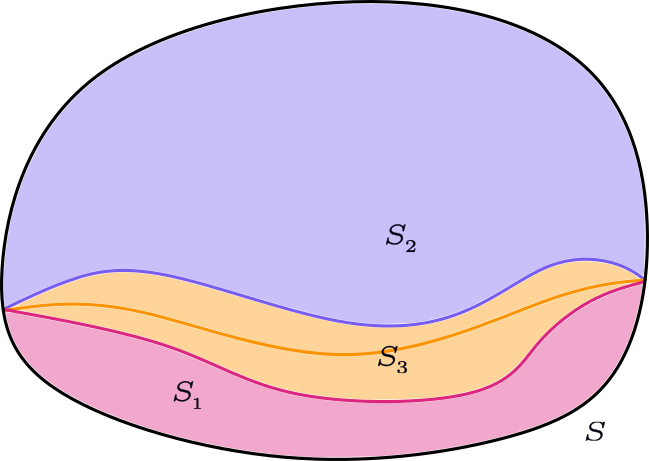
\includegraphics[width=0.55\columnwidth]{Figures/Partitions}\caption{Partitions of convex body}
\end{figure}

\begin{thm}
\label{thm:ball_walk_cond}Let $K$ be a convex body in $\R^{n}$
of diameter $D$ containing the unit ball and with every $u\in K$
having $\ell(u)\ge\ell.$ Then the conductance of the ball walk on
$K$ with step size $\delta$ is 
\[
\Omega\left(\frac{\ell^{2}\delta}{\sqrt{n}D}\right).
\]
\end{thm}

\begin{proof}
Let $K=S_{1}\cup S_{2}$ be a partition into measurable sets. We will
prove that

\begin{eqnarray}
\int_{S_{1}}P_{x}(S_{2})\,dx & \ge & \frac{\ell^{2}\delta}{16\sqrt{n}D}\min\{\vol(S_{1}),\vol(S_{2})\}\label{COND}
\end{eqnarray}
Note that since the uniform distribution is stationary, 
\[
\int_{S_{1}}P_{x}(S_{2})\,dx=\int_{S_{2}}P_{x}(S_{1})\,dx.
\]

Consider the points that are ``deep'' inside these sets, i.e., unlikely
to jump out of the set: 
\[
S_{1}'=\left\{ x\in S_{1}:P_{x}(S_{2})<\frac{\ell}{4}\right\} \mbox{ and }S_{2}'=\left\{ x\in S_{2}:P_{x}(S_{1})<\frac{\ell}{4}\right\} .
\]
Let $S_{3}'$ be the rest i.e., $S_{3}'=K\setminus S_{1}'\setminus S_{2}'$.

Suppose $\vol(S_{1}')<\vol(S_{1})/2$. Then 
\[
\int_{S_{1}}P_{x}(S_{2})\,dx\ge\frac{\ell}{4}\vol(S_{1}\setminus S_{1}')\geq\frac{\ell}{8}\vol(S_{1})
\]
which proves (\ref{COND}).

So we can assume that $\vol(S_{1}')\geq\vol(S_{1})/2$ and similarly
$\vol(S_{2}')\geq\vol(S_{2})/2$. Now, for any $u\in S_{1}'$ and
$v\in S_{2}'$, 
\[
||P_{u}-P_{v}||_{tv}\geq1-P_{u}(S_{2})-P_{v}(S_{1})>1-\frac{\ell}{2}.
\]
Applying Lemma \ref{lem:ONESTEP} with $t=\ell/2$, we get that 
\[
|u-v|\geq\frac{\ell\delta}{2\sqrt{n}}.
\]
Thus $d(S_{1}',S_{2}')\geq\ell\delta/(2\sqrt{n})$. Applying Theorem
\ref{thm:isoD} to the partition $S_{1}',S_{2}',S_{3}'$, we have
\begin{eqnarray*}
\vol(S_{3}') & \geq & \frac{\ell\delta}{\sqrt{n}D}\min\{\vol(S_{1}'),\vol(S_{2}')\}\\
 & \geq & \frac{\ell\delta}{2\sqrt{n}D}\min\{\vol(S_{1}),\vol(S_{2})\}.
\end{eqnarray*}
We can now prove (\ref{COND}) as follows: 
\begin{eqnarray*}
\int_{S_{1}}P_{x}(S_{2})\,dx & = & \frac{1}{2}\int_{S_{1}}P_{x}(S_{2})\,dx+\frac{1}{2}\int_{S_{2}}P_{x}(S_{1})\,dx\\
 & \ge & \frac{1}{2}\vol(S_{3}')\frac{\ell}{4}\\
 & \ge & \frac{\ell^{2}\delta}{16\sqrt{n}D}\min\{\vol(S_{1}),\vol(S_{2})\}.
\end{eqnarray*}

\begin{figure}[H]

\centering{}\includegraphics[width=0.75\columnwidth]{Figures/Lemma_10\lyxdot 10}
\end{figure}

\begin{figure}[H]

\begin{centering}
\includegraphics[width=0.3\columnwidth]{Figures/Lemma_10\lyxdot 10(1)}
\par\end{centering}
\end{figure}
\end{proof}
\begin{cor}
The ball walk in a convex body with local conductance at least $\ell$
everywhere has mixing rate $O(\frac{nD^{2}}{\delta^{2}\ell^{4}})$.
\end{cor}

Using the construction above of adding a small ball to every point
of $K$ gives a lower bound of $\delta=1/n^{3/2}$ and $\ell=\Omega(1)$
and thus a polynomial bound of $O(n^{4}D^{2})$ on the mixing time.
As we will see presently, this can be improved to $n^{2}D^{2}$ by
avoiding the blow-up, and analyzing the \emph{average }local conductance.
The example of starting near a corner (say of a hypercube) shows that
this cannot work in general; however, from a \emph{warm} start, it
will suffice to bound the average local conductance rather than the
minimum. 

\subsection*{Warm Start and $s$-Conductance}

In this section we give a better bound for the conductance of sufficiently
large subsets resulting in the following bound on the mixing rate
of the ball walk.
\begin{thm}
\label{thm:ballwalk_warmstart} From an $O(1)$-warm start, the ball
walk in a convex body with isoperimetric coefficient $\psi$ and containing
a unit ball has a mixing rate of $O(n^{2}/\psi^{2})$ steps. In particular,
if the convex body has diameter $D$, the mixing rate is $O(n^{2}D^{2})$. 
\end{thm}

This is based on two ideas: (1) most points of a convex body containing
a unit ball have large local conductance and we can use $\delta=1/\sqrt{n}$
instead of $1/n^{3/2}$, (2) the $s$-conductance is large and hence
the walk mixes from a suitably warm start.
\begin{lem}
\label{lem:avg-local-conductance} Let $K$ be a convex body containing
a unit ball. For the ball walk with $\delta$ step size, let $K_{\delta}=\left\{ u\in K:\:\ell(u)\ge\frac{3}{4}\right\} $.
Then $K_{\delta}$ is a convex set and $\vol(K_{\delta})\ge(1-2\delta\sqrt{n})\vol(K).$
\end{lem}

\begin{xca}
Prove the first part of the previous lemma.
\end{xca}

The proof of the above lemma will use the following bound on crossing
the boundary of $K$. 
\begin{lem}
Let $L$ be any measurable subset of the boundary of a convex body
$K$ and $S_{L}=\{(x,y):x\in K,y\not\in K,\norm{x-y}\le\delta,[x,y]\cap L\neq\emptyset\}$.
Then, we have 
\[
\vol_{2n}(S_{L})\le\frac{\delta}{(n+1)}\frac{\vol(B^{n-1})}{\vol(B^{n})}\vol_{n-1}(L)\vol(\delta B^{n}).
\]
\end{lem}

\begin{proof}
It suffices to consider the case when $L$ is infinitesimally small;
and then we can assume that the surface of $K$ is locally a hyperplane
and compute the measure of $S_{L}$ explicitly. 
\end{proof}
\begin{thm}
The $s$-conductance of the ball walk with $\delta=\frac{s}{4\sqrt{n}}$
step size in a convex body $K$ with isoperimetric coefficient $\psi$
and containing the unit ball satisfies 
\[
\phi_{s}\gtrsim\frac{s\psi}{n}.
\]
\end{thm}

This proof is similar to that of Theorem \ref{thm:ball_walk_cond},
with one important extension. Rather than applying the argument to
a partition of the original convex body $K$, we restrict the argument
to $K_{\delta}$, the set of points in $K$ that have high local conductance.
Since this subset takes up most of $K$, and is convex, we will be
able to use its isoperimetry to lower bound the conductance. 
\begin{proof}
As before, we consider the following partition of $K$. Let $K=S_{1}\cup S_{2}$
be a partition into measurable sets. We will prove that

\begin{eqnarray}
\int_{S_{1}}P_{x}(S_{2})\,dx & \ge & \frac{\delta\psi}{C\sqrt{n}}\min\{\vol(S_{1})-\frac{s}{2},\vol(S_{2})-\frac{s}{2}\}\label{COND-1}
\end{eqnarray}
Since the uniform distribution is stationary, 
\[
\int_{S_{1}}P_{x}(S_{2})\,dx=\int_{S_{2}}P_{x}(S_{1})\,dx.
\]

Consider the points that are ``deep'' inside these sets: 
\[
S_{1}'=\left\{ x\in S_{1}:P_{x}(S_{2})<\frac{1}{8}\right\} \mbox{ and }S_{2}'=\left\{ x\in S_{2}:P_{x}(S_{1})<\frac{1}{8}\right\} .
\]
Let $S_{3}'$ be the rest i.e., $S_{3}'=K\setminus S_{1}'\setminus S_{2}'$.
Recall that 
\[
K_{\delta}=\left\{ x\in K:\ell(x)\ge\frac{3}{4}\right\} 
\]
and define $S_{i}''=S_{i}'\cap K_{\delta}.$ Note that by Lemma \ref{lem:avg-local-conductance},
for $\delta\le s/(4\sqrt{n})$, 
\[
\vol(S_{i}'')\ge\vol(S_{i}')-s.
\]

Suppose $\vol(S_{1}'')<\vol(S_{1}\cap K_{\delta})/2$. Then 
\[
\int_{S_{1}}P_{x}(S_{2})\,dx\ge\frac{1}{8}\vol(S_{1}\cap K_{\delta}\setminus S_{1}'')\geq\frac{1}{16}\vol(S_{1}\cap K_{\delta})\ge\frac{1}{16}\left(\vol(S_{1})-\frac{s}{2}\right)
\]
which proves (\ref{COND-1}).

So we can assume that $\vol(S_{1}'')\geq\vol(S_{1}\cap K_{\delta})/2$
and similarly $\vol(S_{2}'')\geq\vol(S_{2}\cap K_{\delta})/2$. Now,
for any $u\in S_{1}''$ and $v\in S_{2}''$, 
\[
d_{TV}(P_{u},P_{v})\geq1-P_{u}(S_{2})-P_{v}(S_{1})>1-\frac{1}{4}.
\]
Applying Lemma \ref{lem:ONESTEP} with $t=3/8$, we get that 
\[
|u-v|\geq\frac{3\delta}{8\sqrt{n}}.
\]
Thus $d(S_{1}'',S_{2}'')\geq3\delta/(8\sqrt{n})$. Using the bound
on the isoperimetric coefficient applied to the partition $S_{1}'',S_{2}'',S_{3}''$
of $K_{\delta}$, we have 
\begin{eqnarray*}
\vol(S_{3}'') & \geq & \frac{3\delta\psi}{8\sqrt{n}}\min\{\vol(S_{1}''),\vol(S_{2}'')\}\\
 & \geq & \frac{3\delta\psi}{16\sqrt{n}}\min\{\vol(S_{1})-\frac{s}{2},\vol(S_{2})-\frac{s}{2}\}.
\end{eqnarray*}
We can now prove (\ref{COND-1}) as follows: 
\begin{eqnarray*}
\int_{S_{1}}P_{x}(S_{2})\,dx & = & \frac{1}{2}\int_{S_{1}}P_{x}(S_{2})\,dx+\frac{1}{2}\int_{S_{2}}P_{x}(S_{1})\,dx\\
 & \ge & \frac{1}{2}\vol(S_{3}'')\cdot\frac{1}{8}\\
 & \ge & \frac{3\delta\psi}{256\sqrt{n}}\min\{\vol(S_{1})-\frac{s}{2},\vol(S_{2})-\frac{s}{2}\}
\end{eqnarray*}
which implies that the conductance is at least $3s\psi/(1024n)$.
\end{proof}
The mixing rate then follows by applying Theorem \ref{thm:s-mixing}
and Corollary \ref{cor:s-mixing}.

\subsection*{Tightness of the bound}

The mixing rate of $O(n^{2}D^{2})$ for the ball walk is in fact the
best possible even from a warm start (with the assumption of a unit
ball inside the convex body and diameter $D$). To see this, consider
a cylinder whose cross-section is a unit ball and axis is $[0,D]$
along $e_{1}$. Suppose the starting distribution is uniform in the
part of the cylinder in $[0,D/3]$. Then we claim that to reach the
opposite third of the cylinder needs $\Omega(n^{2}D^{2})$ steps with
high probability. Each step has length at most $\delta$ in a random
direction, and this is about $\delta/\sqrt{n}$ along $e_{1}$. Viewing
this as an unbiased random walk along $e_{1}$, the effective diameter
is $D/(\delta/\sqrt{n})$ and hence the number of steps to cross an
interval of length $D/3$ is $\Omega(nD^{2}/\delta^{2})=\Omega(n^{2}D^{2})$.
\begin{xca}
Prove the above claim rigorously.
\end{xca}


\subsection*{Speedy walk}

In the above analysis of the ball walk, the dependence on the error
parameter $\varepsilon$, the distance to the target distribution,
is polynomial in $1/\varepsilon$ rather than its logarithm. The speedy
walk is a way to improve the analysis. In the speedy walk, at a point
$x$, we sample the next step uniformly from the intersection of $(x+\delta B^{n})\cap K$.
The resulting Markov chain is the subsequence of \emph{proper }steps
of the ball walk.
\begin{xca}
Show that the stationary density of the speedy walk in a convex body
is proportional to the local conductance.
\end{xca}

\begin{thm}
The conductance of the speedy walk is $\Omega(1/(nD))$.
\end{thm}

To analyze the ball walk, we then need to show that the number of
``wasted'' steps is not too many. This follows from the assumption
of a warm start and Lemma \ref{lem:avg-local-conductance}.

\section{Generating a warm start}

To get the mixing rate of $O(n^{2}D^{2})$, we need a warm start,
i.e., a distribution whose density at any point is within $O(1)$
of the target density.

\begin{algorithm2e}[H]

\caption{$\mathtt{Warm\,Start}$}

\SetAlgoLined

Input: membership oracle for $K$ such that $B^{n}\subseteq K\subseteq DB^{n}$.

Let $x$ be a random point in $B^{n}.$ Define $K_{i}=2^{i/n}B^{n}\cap K$.

\For{$i=1,\cdots,n\log D$}{
\begin{enumerate}
\item Use ball walk from $x$ to generate random point $y$ in $K_{i}$.
\item Set $x=y$.
\end{enumerate}
}

\Return $x$.

\end{algorithm2e}

Since $K_{i+1}\subseteq2^{1/n}K_{i}$, we have $\vol(K_{i+1})\le2\vol(K_{i})$
and hence a $2$-warm start is maintained. Once we have a random point
from $K$, subsequent random points can be generated by simply continuing
the ball walk; thus the cost of the warm start is only for the first
sample.

\section{Isotropic Transformation}

The complexity of sampling with the ball walk is polynomial in $n,D$
and $\log(1/\varepsilon)$ to get within $\varepsilon$ of the target
density. This is not a polynomial algorithm since the dependence is
on $D$ and not $\log D$. To get a polynomial algorithm, we need
one more ingredient.

We say that a distribution $Q$ is \emph{isotropic} if $\E_{Q}(x)=0$
and $\E_{Q}(xx^{T})=I$, i.e., the mean is zero and the covariance
matrix (exists and) is the identity. We say that the distribution
is $C$-isotropic if the eigenvalues of its covariance matrix are
in $[\frac{1}{C},C]$. An affine transformation is said to be an \emph{isotropic
transformation} if the resulting distribution is isotropic.

Any distribution with bounded second moments has an isotropic transformation.
It is clear that satisfying the first condition is merely a translation,
so assume the mean is zero. For the second, suppose the covariance
matrix is $\E_{Q}(xx^{T})=A$. Then consider $y=A^{-1/2}x$. It is
easy to see that 
\[
\E(yy^{T})=A^{-1/2}\E\left(xx^{T}\right)A^{-1/2}=I.
\]

For convex bodies, isotropic position comes with a strong guarantee.
\begin{thm}
\label{thm:isotropic-r-R}For a convex body in isotropic position
(i.e., the uniform distribution over the body is isotropic), we have
\[
\sqrt{\frac{n+2}{n}}B^{n}\subseteq K\subseteq\sqrt{n(n+2)}B^{n}.
\]
\end{thm}

\begin{xca}
Show Theorem \ref{thm:isotropic-r-R} up to absolute constants, i.e.,
show that for any convex body in isotropic position, it contains and
is contained in origin-centered balls of radii $\Omega(1)$ and $O(n)$,
respectively. Moreover, give an isotropic convex body where both of
these bounds are tight.
\end{xca}

Thus the effective diameter is $O(n)$. If we could place a convex
body in isotropic position before sampling, we would have a poly($n$)
algorithm. In fact, it is even better than this as most points are
within distance $O(\sqrt{n})$ of the center of gravity. We quote
a theorem due to Paouris.
\begin{thm}
For an isotropic logconcave density $p$ in $\R^{n}$ and any $t\ge1$,
\[
\Pr_{p}\left(\norm x\ge ct\sqrt{n}\right)\le e^{-t\sqrt{n}}.
\]
\end{thm}

How to compute an isotropic transformation? This is easy, from the
definition, all we need is to estimate its covariance matrix, which
can be done from random samples. Thus, if we could sample $K$, we
can compute an isotropic transformation for it. This appears cyclic
-- we need isotropy for efficient sampling and efficient sampling
for isotropy. The solution is simply to bootstrap them.

\begin{algorithm2e}[H]

\caption{$\mathtt{IsotropicTransform}$}

\SetAlgoLined

Input: membership oracle for $K$ such that $B^{n}\subseteq K\subseteq RB^{n}$.

Let $x$ be a random point in $B^{n}$, $A=I$ and $K_{i}=2^{i/n}B^{n}\cap K$.

\For{$i=1,\cdots,n\log R$}{
\begin{enumerate}
\item Use the ball walk from $x$ to generate $N$ random points $x_{1}\ldots x_{N}$
in $AK_{i}$.
\item Compute $C=\frac{1}{N}\sum^{N}_{i=1}x_{i}x^{T}_{i}$ and set $A=C^{-1/2}A$.
\item Set $x=x_{N}$.
\end{enumerate}
}

\Return $x$.

\end{algorithm2e}

We will choose $N$ large enough so that after the transformation
$K_{i}$ is $2$-isotropic. We can bound $N$ as follows.
\begin{xca}
Show that if $K$ is isotropic, then with $N=O(n^{2})$, the matrix
$A=\frac{1}{N}\sum^{N}_{i=1}x_{i}x^{T}_{i}$ for $N$ random samples
from $K$ satisfies $\norm{A-I}_{\op}\le0.5.$

A tight bound on the sample complexity was established by \cite{adamczak2010quantitative}
(see also \cite{Bourgain96,Rudelson1999,srivastava2013covariance}).
\end{xca}

\begin{thm}
For an isotropic logconcave distribution $Q$ in $\R^{n}$, the empirical
covariance matrix from $N=O(n)$ random samples satisfies $\norm{A-I}_{\op}\le0.5$.
\end{thm}

\begin{lem}
If $K_{i}$ is $C$-isotropic, then $K_{i+1}$ is $3C$-isotropic.
\end{lem}

Thus the overall algorithm needs $O(n\log R)$ phases, with $O(n)$
samples in each phase from a near-isotropic distribution, and thus
poly($n$) steps per sample.
\begin{thm}
\label{thm:convex_body_rounding} Any convex body $K$ with $B_{n}\subseteq K\subseteq RB_{n}$
given by a membership oracle can be put in $2$-isotropic position
with probability at least $9/10$, using $\widetilde{O}(n^{4})$ oracle
queries.  
\end{thm}


\section{Isoperimetry via localization}

Theorem \ref{thm:isoD} was refined by KLS \cite{Kannan1995} as follows
(we state it here for logconcave densities).
\begin{thm}
For any partition $S_{1},S_{2},S_{3}$ of $\R^{n}$, and any logconcave
measure $\mu$ in $\R^{n}$, 
\[
\mu(S_{3})\ge\frac{\ln2}{\E_{\mu}(\norm{x-\bar{x}})}\min\left\{ \mu(S_{1}),\mu(S_{2})\right\} .
\]
\end{thm}

Thus, for a (near-)isotropic distribution, the diameter can be replaced
by $O(\sqrt{n})$ and this gives a bound of $O(n^{3})$ from a warm
start. One way to summarize the analysis so far is that the complexity
of sampling a convex body (and in fact a logconcave density) from
a warm start is $O^{*}(n^{2}/\psi^{2})$ where $\psi$ is the isoperimetric
ratio of the convex body. In other words, the expansion of the Markov
chain reduces to the expansion of the target logconcave density. It
then becomes a natural question to find the best possible estimate
for the isoperimetric ratio. KLS also provided a conjecture for this.
\begin{conjecture}[KLS Hyperplane Conjecture]
 The isoperimetric ratio of any isotropic logconcave density in $\R^{n}$
is $\Omega(1)$.
\end{conjecture}

The bound of the conjecture holds for all halfspace induced subsets.
So the conjecture says that the worst isoperimetry is achieved up
to a constant factor by a halfspace (this version does not need isotropic
position). Here we discuss a powerful technique for proving such inequalities.

Classical proofs of isoperimetry for special distributions are based
on different types of symmetrization that effectively identify the
extremal subsets. Bounding the Cheeger constant for general convex
bodies and logconcave densities is more complicated since the extremal
sets can be nonlinear and hard to describe precisely, due to the trade-off
between minimizing the boundary measure of a subset and utilizing
as much of the ``external'' boundary as possible. The main technique
to prove bounds in the general setting has been \emph{localization},
a method to reduce inequalities in high dimension to inequalities
in one dimension. We now describe this technique with a few applications. 

\subsection{Localization}

We will sketch a proof of the following theorem to illustrate the
use of localization. This theorem was also proved by Karzanov and
Khachiyan \cite{KarzanovK91} using a different, more direct approach.
\begin{thm}[\cite{DyerF90,LS90,KarzanovK91}]
\label{ISO2}Let $f$ be a logconcave function whose support has
diameter $D$ and let $\pi_{f}$ be the induced measure. Then for
any partition of $\R^{n}$ into measurable sets $S_{1},S_{2},S_{3}$,

\[
\pi_{f}(S_{3})\geq\frac{2d(S_{1},S_{2})}{D}\min\{\pi_{f}(S_{1}),\pi_{f}(S_{2})\}.
\]
\end{thm}

Before discussing the proof, we note that there is a variant of this
result in the Riemannian setting.
\begin{thm}[\cite{li1980estimates}]
If $K\subset(M,g)$ is a locally convex bounded domain with smooth
boundary, diameter $D$ and $Ric_{g}\geq0$, then the Poincar� constant
is at least $\frac{\pi^{2}}{4D^{2}}$, i.e., for any $g$ with $\int g=0$,
we have that
\[
\int\left|\nabla g(x)\right|^{2}dx\geq\frac{\pi^{2}}{4D^{2}}\int g(x)^{2}dx.
\]
\end{thm}

For the case of convex bodies in $\Rn$, this result is equivalent
to Theorem \ref{ISO2} up to a constant. One benefit of localization
is that it does not require a carefully crafted potential. Localization
has been extended to the Riemannian setting \cite{klartag2017needle}.
The origins of this method were in a paper by Payne and Weinberger
\cite{payne1960optimal}. 

We begin the proof of Theorem \ref{ISO2}. For a proof by contradiction,
let us assume the converse of its conclusion, i.e., for some partition
$S_{1},S_{2},S_{3}$ of $\R^{n}$ and logconcave density $f$, assume
that

\[
\int_{S_{3}}f(x)\,dx<C\int_{S_{1}}f(x)\,dx\quad\mbox{ and }\quad\int_{S_{3}}f(x)\,dx<C\int_{S_{2}}f(x)\,dx
\]
where $C=2d(S_{1},S_{2})/D$. This can be reformulated as 

\begin{equation}
\int_{\R^{n}}g(x)\,dx>0\quad\mbox{ and }\quad\int_{\R^{n}}h(x)\,dx>0\label{eq:1}
\end{equation}
where 
\[
g(x)=\begin{cases}
Cf(x) & \mbox{ if }x\in S_{1},\\
0 & \mbox{ if }x\in S_{2},\\
-f(x) & \mbox{ if }x\in S_{3}.
\end{cases}\quad\mbox{ and }\quad h(x)=\begin{cases}
0 & \mbox{ if }x\in S_{1},\\
Cf(x) & \mbox{ if }x\in S_{2},\\
-f(x) & \mbox{ if }x\in S_{3}.
\end{cases}
\]
 These inequalities are for functions in $\R^{n}$. The next lemma
will help us analyze them.
\begin{lem}[Localization Lemma \cite{Kannan1995}]
\label{lem:LOCALIZATION}Let $g,h:\R^{n}\rightarrow\R$ be lower
semi-continuous integrable functions such that 
\[
\int_{\R^{n}}g(x)\,dx>0\quad\mbox{ and }\quad\int_{\R^{n}}h(x)\,dx>0.
\]
 Then there exist two points $a,b\in\R^{n}$ and an affine function
$\ell:[0,1]\rightarrow\R_{+}$ such that 
\[
\int^{1}_{0}\ell(t)^{n-1}g((1-t)a+tb)\,dt>0\quad\mbox{ and }\quad\int^{1}_{0}\ell(t)^{n-1}h((1-t)a+tb)\,dt>0.
\]
\end{lem}

The points $a,b$ represent an interval and one may think of $\ell(t)^{n-1}$
as proportional to the cross-sectional area of an infinitesimal cone.
The lemma says that over this cone truncated at $a$ and $b$, the
integrals of $g$ and $h$ are positive. Also, without loss of generality,
we can assume that $a,b$ are in the union of the supports of $g$
and $h$.  An equivalent alternative version of the lemma has equality
for one function and inequality for the other i.e., $\int g=0,\int h>0$
for both the assumption and the conclusion \cite[Corollary 2.4]{Kannan1995}. 
\begin{proof}
Without loss of generality, we can assume that the functions $g,h$
are continuous. This is because they are limits of monotone increasing
sequences of continuous functions $g_{k},h_{k}$ where 
\[
\lim_{k\rightarrow\infty}\int g_{k}=\int g>0\quad\text{and}\quad\lim_{k\rightarrow\infty}\int h_{k}=\int h>0\,.
\]
Hence there exists $k_{0}$ such that for all $k\ge k_{0}$, $\int g_{k},\int h_{k}>0$.
We can apply the lemma to these and derive the conclusion for $g,h$.
Moreover, it suffices to prove the final conclusion with $\ge0$,
as we can always consider $g-\gamma,h-\gamma>0$ for some strictly
positive continuous small enough function $\gamma$.

The main idea of the proof is ``bisection''. Let $H$ be any halfspace
such that 
\[
\int_{H}g(x)\,dx=\frac{1}{2}\int g(x)\,dx\,.
\]
Let us call this a bisecting halfspace. Now either 
\[
\int_{H}h(x)\,dx>0\quad\mbox{ or }\quad\int_{\R^{n}\setminus H}h(x)\,dx>0\,.
\]
Thus, either $H$ or its complement will have positive integrals for
both $g$ and $h$, reducing the domain of the integrals from $\R^{n}$
to a halfspace. If we could repeat this, we might hope to reduce the
dimensionality of the domain. For any $(n-2)$-dimensional affine
subspace $L$, there is a bisecting halfspace containing $L$ in its
bounding hyperplane. To see this, let $H$ be a halfspace containing
$L$ in its boundary. Rotating $H$ about $L$ we get a family of
halfspaces with the same property. This family includes $H'$, the
complementary halfspace of $H$. The function $\int_{H}g-\int_{\R^{n}\setminus H}g$
switches sign from $H$ to $H'$. Since this is a continuous family,
there must be a halfspace for which the function is zero.

If we take all $(n-2)$-dimensional affine subspaces defined by $\{x\in\Rn:\ x_{i}=r_{1},\,x_{j}=r_{2}\}$
where $r_{1},r_{2}$ are rational, then the intersection of all the
corresponding bisecting halfspaces is a line or a point (by choosing
only rational values for $x_{i}$, we are considering a countable
intersection). To see why it is a line or a point, assume we are left
with a two or higher dimensional set. Since the intersection is convex,
there is a point in its interior with at least two coordinates that
are rational, say $x_{1}=r_{1}$ and $x_{2}=r_{2}$. But then there
is a bisecting halfspace $H$ that contains the affine subspace given
by $x_{1}=r_{1},\,x_{2}=r_{2}$ in its boundary, and so it properly
partitions the current set. Thus the limit of this bisection process
is a function supported on an interval (which could be a single point).

In fact, this gives a sequence of convex bodies, where $K_{0}$ can
be a large enough ball, and $K_{i+1}=K_{i}\cap H_{i}$, the bisecting
halfspace found at step $i$. Define $K=\cap_{i}K_{i}$. We have just
argued that $K$ is an interval $[a,b]$. If $a=b$, then the conclusion
follows by continuity with $\ell=1$. So assume $a\neq b$.

If $a\neq b$, then we may assume $a=0$ and $b=e_{1}$ (by scaling
and translation). For a slice $Z_{t}:=\{x\in\Rn:x_{1}=t\}$ (here
$t\in\R$), consider the following sequence of functions over $[0,1]$
for $m\ge0$: 
\[
\psi_{m}(t):=\left(\frac{\vol_{n-1}(K_{m}\cap Z_{t})}{\vol_{n}(K_{m})}\right)^{\frac{1}{n-1}}\,.
\]
Note that $\int\psi_{m}(t)^{n-1}\,dt=1$. For $\alpha_{m}:=\min\{x_{1}:x\in K_{m}\}$
and $\beta_{m}:=\max\{x_{1}:x\in K_{m}\}$, we have $\alpha_{m}\le0,\beta_{m}\ge1$
and $\alpha_{m}\rightarrow0,\beta_{m}\rightarrow1$. Moreover, by
the Brunn--Minkowski inequality (Thm \ref{thm:Brunn-Minkowski})
$\psi_{i}$ is non-negative concave on its support. Then we can take
a subsequence of indices $m$ for which $\psi_{m}$ converges to a
limit. To see this, note that $\psi_{m}$ is uniformly equicontinuous
in every interval $[s,t]$ with $0<s<t<1$, and by the Arzela--Ascoli
theorem, the sequence has a pointwise convergent subsequence. The
limit $\psi$ is also non-negative concave with the same integral,
i.e., $\int\psi(t)^{n-1}\,dt=1$.

Note that for $x=(y,t)\in\R^{n-1}\times\R$,
\[
\frac{1}{\vol(K_{m})}\int_{K_{m}}g(x)\,dx=\int^{\beta_{m}}_{\alpha_{m}}\frac{1}{\vol_{n-1}(K_{m}\cap Z_{t})}\int_{K_{m}\cap Z_{t}}g(y,t)\,dy\,\psi_{m}(t)^{n-1}\,dt\,.
\]
Since the LHS is nonnegative, and the RHS approaches $\int^{1}_{0}g(0,t)\,\psi(t)^{n-1}\,dt$,
we obtain that

\[
\int^{1}_{0}\psi(t)^{n-1}\,g(te_{1})\,dt\ge0\quad\text{and}\quad\int^{1}_{0}\psi(t)^{n-1}\,h(te_{1})\,dt\ge0\,.
\]

The last part of the proof is to argue that we can take $\psi$ to
be a nonnegative linear function, reducing the extremal functions
to a small parameter family (namely, $a,b,$ and the values of the
function at $a$ and $b$). To do this consider a $\psi$ that has
(i) minimal support $\norm{a-b}$; without loss of generality, assume
$a=0,b=e_{1}$, and (ii) is linear in the segment $[\alpha,\beta]$
for $0\le\alpha\le\beta\le1$ such that $\beta-\alpha$ is maximal.
It will be useful to view $\psi$ as defining a convex body $K'$
whose slices are simplices:
\[
0\le t\le1,\quad x_{1},\ldots,x_{n}\ge0,\quad x_{2}+\ldots+x_{n}\le\psi(t)\,.
\]
In words, the slice of $K'$ at $x_{1}=t$ is the standard simplex
given by the convex hull of 
\[
\{te_{1},te_{1}+\psi(t)\,e_{2},\ldots,te_{1}+\psi(t)\,e_{i},\ldots,te_{1}+\psi(t)\,e_{n}\}\,.
\]
The slice at $x_{1}=t$ has volume $\psi(t)^{n-1}/(n-1)!$. Hence,
if we define $\hat{g}(x)=g(x_{1}e_{1})$ and $\hat{h}(x)=h(x_{1}e_{1})$,
then 
\[
\int_{\K'}\hat{g}=\frac{1}{(n-1)!}\int^{1}_{0}\psi(t)^{n-1}\,g(te_{1})\,dt\ge0
\]
and similarly for $\int_{\K'}\hat{h}\ge0$. Without loss of generality,
we can assume that $\int_{\K'}\hat{g}=0$.

\begin{figure}[H]
\centering{}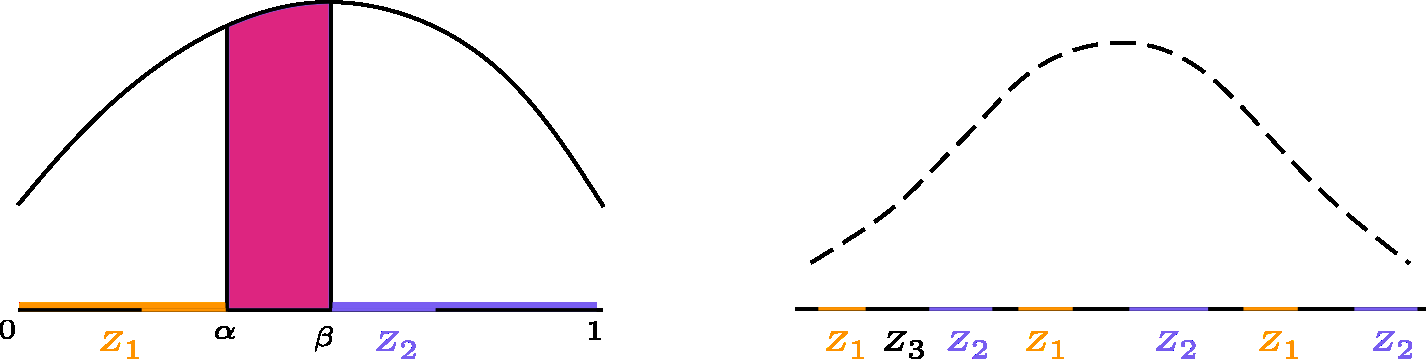
\includegraphics[width=0.5\textwidth]{Figures/concave-to-affine}\caption{Going to an affine needle}
\end{figure}

The overall proof idea is to subdivide $K'$ with a hyperplane in
such a way that one of the resulting halfspaces satisfies the same
two inequalities but violates either (i) or (ii). To choose this hyperplane,
we first fix an $(n-2)$-dimensional subspace $A=\left\{ x:x_{1}=\sigma,\,x_{2}+\ldots+x_{n}=\tau\right\} $
where $0<\sigma<1$ and $\tau>0$. The hyperplane will be chosen to
contain $A$ and bisect the function $\hat{g}$ so that $\int_{L}\hat{g}=\int_{L'}\hat{g}=0$
in both resulting convex bodies $L$ and $L'$. Suppose $\int_{L}h\ge0$.
Then we can infer that $L$ must intersect both $Z_{0}$ and $Z_{1}$,
otherwise the function $\psi$ restricted to $L$ contradicts the
(i), the minimality of the support of $\psi$. 

We now consider 3 cases:
\begin{enumerate}
\item $\psi(0)=\psi(1)=0$. For this case, let $\sigma=1/2$. Then $L$
must contain the segment $[0,1]\,e_{1}$, for any $\tau>0$, else
it contradicts (i). Then there is a linear function $\ell(t)$ with
$\ell(0),\ell(1)\ge0,\ell(1/2)=\tau$ such that the function $\psi$
restricted to $L$ is $\psi_{L}(t)=\min\{\psi(t),\ell(t)\}$. But
then as $\tau\rightarrow0$, $\ell(t)$ tends to zero in the interval
$[0,1]$ and so $\psi_{L}$ is linear in a larger sub-interval tending
to $[0,1]$ contradicting (ii).
\item $\psi(0)=0,\psi(1)>0$. For this case, consider $\tau=\psi(1)\,\sigma$.
Now if $L$ does not contain $[0,1]\,e_{1}$, then $\psi_{L}(0)=\psi_{L}(1)=0$,
taking us back to the first case. Otherwise, $\psi_{L}$ is linear
in the interval $[\sigma,1]$ and hence for small enough $\sigma$
this again contradicts (ii).
\item $\psi(0),\psi(1)>0$. Consider the family of continuous, nonnegative,
convex functions $\eta:[0,1]\to\R_{+}$ satisfying $\eta(t)\le\psi(t)$
for all $t\in[0,1]$. Let 
\[
K_{\eta}=K'\cap\{x:x_{2}+\ldots+x_{n}\ge\eta(x_{1})\}=\{x\in\R_{+}:x_{1}\in[0,1],\,\eta(x_{1})\le x_{2}+\ldots+x_{n}\le\psi(x_{1})\}\,.
\]
Then we choose $\eta$ so that (iii) $\int^{1}_{0}\eta(t)\,dt$ is
maximal while still satisfying 
\[
\int_{\K_{\eta}}\hat{g}=0\,,\quad\int_{\K_{\eta}}\hat{h}\ge0\,.
\]
Then, we can assume that $\eta(0)<\psi(0),\eta(1)<\psi(1)$. If not,
we consider the function $\psi-\eta$ and this takes us back to one
of the previous cases. Now let $(\sigma,\tau)$ be the intersection
of the segments $[(0,\eta(0)),(1,\psi(1))]$ and $[(0,\psi(0)),(1,\eta(1))]$.
Let $M,M'$ be the partition of $K_{\eta}$ such that $M$ does not
contain $[0,1]\,e_{1}$ and
\[
\int_{M}\hat{g}=\int_{M'}\hat{g}=0\,.
\]
Then, if $\int_{M}\hat{h}\ge0$, this contradicts (iii), the maximality
of $\eta$. Hence, $\int_{M}\hat{h}<0$ and the truncated cone $K'\setminus M$
satisfies 
\[
\int_{K'\setminus M}\hat{g}=\int_{K'}\hat{g}-\int_{M}\hat{g}=0\qquad\int_{K'\setminus M}\hat{h}=\int_{K'}\hat{h}-\int_{M}\hat{h}\ge0\,,
\]
which contradicts (ii), the maximality of the linear subinterval of
$\psi$. 
\end{enumerate}
This completes the proof. 
\end{proof}
Going back to the proof of Theorem \ref{ISO2}, we can apply the localization
lemma to get an interval $[a,b]$ and an affine function $\ell$ such
that 
\begin{equation}
\int^{1}_{0}\ell(t)^{n-1}g((1-t)a+tb)\,dt>0\quad\mbox{ and }\quad\int^{1}_{0}\ell(t)^{n-1}h((1-t)a+tb)\,dt>0.\label{AFTERLEMMA}
\end{equation}
The functions $g,h$ as we have defined them are not lower semi-continuous.
However, this can be addressed by expanding $S_{1}$ and $S_{2}$
slightly so as to make them open sets, and making the support of $f$
an open set. Since we are proving strict inequalities, these modifications
do not affect the conclusion.

\begin{figure}[H]

\begin{centering}
\includegraphics[width=0.75\columnwidth]{Figures/Lemma_10\lyxdot 30}
\par\end{centering}
\centering{}
\end{figure}

Let us partition $[0,1]$ into $Z_{1},Z_{2},Z_{3}$ as follows: 
\[
Z_{i}=\{t\in[0,1]\,:\,(1-t)a+tb\in S_{i}\}.
\]
Note that for any pair of points $u\in Z_{1},v\in Z_{2},\,|u-v|\ge d(S_{1},S_{2})/D$.
We can rewrite (\ref{AFTERLEMMA}) as 
\[
\int_{Z_{3}}\ell(t)^{n-1}f((1-t)a+tb)\,dt<C\int_{Z_{1}}\ell(t)^{n-1}f((1-t)a+tb)\,dt
\]
and 
\[
\int_{Z_{3}}\ell(t)^{n-1}f((1-t)a+tb)\,dt<C\int_{Z_{2}}\ell(t)^{n-1}f((1-t)a+tb)\,dt.
\]
The functions $f$ and $\ell(\cdot)^{n-1}$ are both logconcave, so
$F(t)=\ell(t)^{n-1}f((1-t)a+tb)$ is also logconcave. We get, 
\begin{equation}
\int_{Z_{3}}F(t)\,dt<C\min\left\{ \int_{Z_{1}}F(t)\,dt,\int_{Z_{2}}F(t)\,dt\right\} .\label{FEQ}
\end{equation}
Now consider what Theorem \ref{ISO2} asserts for the function $F(t)$
over the interval $[0,1]$ and the partition $Z_{1},Z_{2},Z_{3}$:
\begin{equation}
\int_{Z_{3}}F(t)\,dt\geq2d(Z_{1},Z_{2})\min\left\{ \int_{Z_{1}}F(t)\,dt,\int_{Z_{2}}F(t)\,dt\right\} .\label{FEQ2}
\end{equation}
We have substituted $1$ for the diameter of the interval $[0,1]$.
Also, $2d(Z_{1},Z_{2})\geq2d(S_{1},S_{2})/D=C$. Thus, Theorem \ref{ISO2}
applied to the function $F(t)$ contradicts (\ref{FEQ}). To prove
the theorem in general, it suffices to prove it in the one-dimensional
case. A combinatorial argument reduces this to the case when each
$Z_{i}$ is a single interval. Proving the resulting inequality up
to a factor of $2$ is a simple exercise and uses only the unimodality
of $F$. The improvement to the tight bound requires one-dimensional
logconcavity. This completes the proof of Theorem \ref{ISO2}.

The localization lemma has been used to prove a variety of isoperimetric
inequalities. The next theorem is a refinement of Theorem \ref{ISO2},
replacing the diameter by the square-root of the expected squared
distance of a random point from the mean. For an isotropic distribution
this is an improvement from $n$ to $\sqrt{n}$. This theorem was
proved by Kannan-Lov�sz-Simonovits in the same paper in which they
proposed the KLS conjecture. 
\begin{thm}[\cite{Kannan1995}]
\label{thm:KLS_thm} For any logconcave density $p$ in $\R^{n}$
with covariance matrix $A$, the KLS constant satisfies
\[
\psi_{p}\gtrsim\frac{1}{\sqrt{\tr(A)}}.
\]
\end{thm}

The next theorem shows that the KLS conjecture is true for an important
family of distributions. The proof is again by localization \cite{CV2014},
and the one-dimensional inequality obtained is a Brascamp-Lieb Theorem.
We note that the same theorem can be obtained by other means \cite{Ledoux1999}.
\begin{thm}
\label{thm:Gaussian-iso}Let $h(x)=f(x)e^{-\frac{1}{2}x^{\top}Bx}/\int f(y)e^{-\frac{1}{2}y^{\top}By}dy$
where $f:\R^{n}\rightarrow\R_{+}$ is an integrable logconcave function
and $B$ is positive definite. Then $h$ is logconcave and for any
measurable subset $S$ of $\R^{n}$,
\[
\frac{h(\partial S)}{\min\left\{ h(S),h\left(\R^{n}\setminus S\right)\right\} }\gtrsim\frac{1}{\norm{B^{-1}}^{\frac{1}{2}}_{\op}}.
\]
In other words, the expansion of h is $\Omega(\norm{B^{-1}}^{-\frac{1}{2}}_{\op})$.
\end{thm}

The analysis of the Gaussian Cooling algorithm for volume computation
\cite{CV2015} uses localization.

Next we mention an application to the anti-concentration of polynomials.
This is a corollary of a more general result by Carbery and Wright.
\begin{thm}[\cite{carbery2001distributional}]
Let $q$ be a degree $d$ polynomial in $\R^{n}$. Then for a convex
body $K\subset\R^{n}$ of volume $1$, any $\epsilon>0$, and $x$
drawn uniformly from $K$, 
\[
\Pr_{x\sim K}\left(|q(x)|\le\epsilon\max_{K}|q(x)|\right)\lesssim\epsilon^{\frac{1}{d}}d
\]
\end{thm}


\subsection{Alternative formulations of Localization}

Here we give some alternative equivalent versions of Lemma \ref{lem:LOCALIZATION}
which are sometimes more convenient in applications.

The first is in terms of single inequality on products of integrals.
Note that an $n$-dimensional needle $N$ is specified by a pair of
points $a,b\in\R^{n}$ and a linear function $\ell:[0,1]\rightarrow\R_{+}$.
The integral over a needle is defined as 
\[
\int_{N}f=\int^{1}_{0}f((1-t)a+tb)\ell(t)^{n-1}\,dt.
\]

\begin{lem}[Localization: Product form]
 Let $f_{1},f_{2},f_{3},f_{4}:\R^{n}\rightarrow\R_{+}$ be nonnegative,
continuous functions. Then the following are equivalent:
\end{lem}

\begin{enumerate}
\item For every convex body $K\subset\R^{n},$ we have
\[
\int_{K}f_{1}\int_{K}f_{2}\le\int_{K}f_{3}\int_{K}f_{4}.
\]
\item For every needle $N$ in $\R^{n}$, we have
\[
\int_{N}f_{1}\int_{N}f_{2}\le\int_{N}f_{3}\int_{N}f_{4}.
\]
\end{enumerate}
The next version is in terms of exponential needles, i.e., we replace
the linear functions obtained in the one-dimensional case in Lemma
\ref{lem:LOCALIZATION} with truncated exponentials. 
\begin{lem}[Localization: exponential needles]
\label{lem:localization_exp_needles} Let $f_{1},f_{2},f_{3},f_{4}:\R^{n}\rightarrow\R_{+}$
be nonnegative, continuous functions and $\alpha,\beta>0$. Then,
the following are equivalent:
\end{lem}

\begin{enumerate}
\item For every logconcave function $F:\R^{n}\rightarrow\R_{+}$, we have
\[
\left(\int_{\R^{n}}F(x)\,f_{1}(x)\,dx\right)^{\alpha}\left(\int_{\R^{n}}F(x)\,f_{2}(x)\,dx\right)^{\beta}\le\left(\int_{\R^{n}}F(x)\,f_{3}(x)\,dx\right)^{\alpha}\left(\int_{\R^{n}}F(x)\,f_{4}(x)\,dx\right)^{\beta}\,.
\]
\item For every interval $a,b\in\R^{n}$ and every $\gamma\in\R$, we have
\[
\left(\int^{1}_{0}e^{\gamma t}f_{1}(t)\,dt\right)^{\alpha}\left(\int^{1}_{0}e^{\gamma t}f_{2}(t)\,dt\right)^{\beta}\le\left(\int^{1}_{0}e^{\gamma t}f_{3}(t)\,dt\right)^{\alpha}\left(\int^{1}_{0}e^{\gamma t}f_{4}(t)\,dt\right)^{\beta}\,
\]
where $f_{i}(t)=f_{i}((1-t)a+tb)$.
\end{enumerate}
\begin{rem}
We can also write the exponential needle version of localization in
terms of two inequalities or one equality and one inequality: For
every logconcave $\ensuremath{F:\R\rightarrow\R_{+}}$
\[
\int^{b}_{a}Ff_{1}=0,\ \int^{b}_{a}Ff_{2}>0
\]
if and only if for every subinterval $\ensuremath{[a',b']\subseteq[a,b]}$,
and every $\gamma\in\R$, 
\[
\int^{b'}_{a'}e^{\gamma t}f_{1}=0,\ \int^{b'}_{a'}e^{\gamma t}f_{2}>0.
\]

We conclude this section with a nice interpretation of the localization
lemma by Fradelizi and Guedon. They also give a version that extends
localization to multiple inequalities.
\end{rem}

\begin{thm}[Reformulated Localization Lemma \cite{fradelizi2004extreme}]
Let $K$ be a compact convex set in $\Rn$ and $f$ be an upper semi-continuous
function. Let $P_{f}$ be the set of logconcave distributions $\mu$
supported by $K$ satisfying $\int fd\mu\geq0$. The set of extreme
points of $\text{conv}\,P_{f}$ is exactly:
\begin{enumerate}
\item the Dirac measure at points $x$ such that $f(x)\geq0$, or
\item the distributions $v$ that satisfy
\begin{enumerate}
\item density function is of the form $e^{\ell}$ with linear $\ell$,
\item support is a segment $[a,b]\subset K$,
\item $\int fdv=0$,
\item $\int^{x}_{a}fdv>0$ for $x\in(a,b)$ or $\int^{b}_{x}fdv>0$ for
$x\in(a,b)$.
\end{enumerate}
\end{enumerate}
\end{thm}

Since we know the maximizer of any convex function is at extreme points,
this shows that one can optimize $\max_{\mu\in P_{f}}\Phi(\mu)$ for
any convex $\Phi$ by only checking Dirac measures and log-affine
functions.

\section{Hit-and-Run}

The ball walk does not mix rapidly from all starting points in arbitrary
convex bodies. While this hurdle can be overcome by starting with
a deep point and carefully maintaining a warm start, it is natural
to ask if there is a simple process that truly does mix rapidly from
any starting point. Hit-and-Run satisfies this requirement.

\begin{figure}[h]
\centering{}\includegraphics[width=0.7\textwidth]{Figures/Section_10\lyxdot 1}\caption{Hit-and-Run Algorithm}
\end{figure}

\begin{algorithm2e}[H]

\caption{$\mathtt{Hit\mbox{-}and\mbox{-}Run}$}

\SetAlgoLined

Input: starting point $x_{0}$ in a convex body $K$.

Repeat $T$ times: at current point $x$,
\begin{enumerate}
\item Pick a uniform random direction $\ell$ through $x$.
\item Go to a uniformly random point $y$ on the chord of $K$ induced by
$\ell$.
\end{enumerate}
\Return $x$.

\end{algorithm2e}

Since hit-and-run is a symmetric Markov chain, the uniform distribution
on $K$ is stationary for it. To sample from a general density proportional
to $f(x)$, in Step 2, we sample $y$ according to the density proportional
to $f$ restricted to the random line $\ell$. 
\begin{xca}
Show that Hit-and-Run satisfies detailed balance. 
\end{xca}

Next we give a formula for the next step distribution from a point
$u$.
\begin{lem}
\label{lem:har-next-step}The next step distribution of Hit-and-Run
from a point $u$ is given by
\[
P_{u}(A)=\frac{2}{\vol(S^{n-1})}\int_{A}\frac{dx}{\norm{x-u}^{n-1}\ell(u,x)}
\]
where $A$ is any measurable subset of $K$ and $\ell(u,x)$ is the
length of the chord in $K$ through $u$ and $x$.

\begin{figure}[h]
\begin{centering}
\includegraphics[width=0.7\textwidth]{Figures/Lemma_10\lyxdot 35}
\par\end{centering}
\end{figure}
\end{lem}

\begin{xca}
Prove Lemma \ref{lem:har-next-step}.
\end{xca}

The main theorem of this section is the following \cite{LV3}.

\begin{figure}[h]
\begin{centering}
\includegraphics[width=0.6\textwidth]{Figures/Thrm_10\lyxdot 37}\caption{Hit-and-Run from a corner}
\par\end{centering}
\end{figure}

\begin{thm}
\cite{LV3}\label{thm:har-cond} The conductance of Hit-and-Run in
a convex body $K$ containing the unit ball and of diameter $D$ is
$\Omega(1/(nD))$.
\end{thm}

This implies a mixing time of $O\left(n^{2}D^{2}\log(M/\varepsilon)\right)$
to get to within distance $\varepsilon$ of the target density starting
from an $M$-warm initial density. By taking one step from the initial
point, we can bound $M$ by $(D/d)^{n}$ where $d$ is the minimum
distance of the starting point from the boundary. Hence this gives
a bound of $\tilde{O}(n^{3}D^{2})$ from \emph{any} interior starting
point.

The proof of the theorem follows the same high-level outline as that
of the ball walk, needing two major ingredients, namely, one-step
coupling and isoperimetry. Notably, the isoperimetry is for a non-Euclidean
notion of distance. We begin with some suitable definitions. 

Define the ``median'' step-size function $F$ by setting $F(x)$
to satisfy
\[
\Pr(\norm{x-y}\le F(x))=\frac{1}{8}
\]
where $y$ is a random step from $x$.

We also need a non-Euclidean notion of distance, namely the classical
cross-ratio distance. For points $u,v$ in $K$, inducing a chord
$[p,q]$ with these points in the order $p,u,v,q$, the cross-ratio
distance is
\[
d_{K}(u,v)=\frac{\norm{u-v}\norm{p-q}}{\norm{p-u}\norm{v-q}}.
\]

It is related to the Hilbert distance (which is a true distance) as
follows: 
\[
d_{H}(u,v)=\ln\left(1+d_{K}(u,v)\right).
\]

The first ingredient shows that if two points are close geometrically,
then their next-step distributions have significant overlap.
\begin{lem}
\cite{Lovasz1998}\label{lem:har_one_step} For two points $u,v\in K$
with 
\[
d_{K}(u,v)<\frac{1}{8}\mbox{ and }\norm{u-v}\le\frac{2}{\sqrt{n}}\max\left\{ F(u),F(v)\right\} 
\]
we have $d_{TV}(P_{u},P_{v})<1-\frac{1}{500}$.
\end{lem}

The second ingredient is an isoperimetric inequality (independent
of any algorithm). The cross-ratio distance has a nice isoperimetry
inequality.

\begin{figure}[h]

\begin{centering}
\includegraphics[width=0.6\textwidth]{Figures/Thrm_10\lyxdot 39}
\par\end{centering}
\end{figure}

\begin{thm}
\label{thm:iso-cross-ratio}For any partition $S_{1},S_{2},S_{3}$
of a convex body $K$, 
\[
\vol(S_{3})\ge d_{K}(S_{1},S_{2})\frac{\vol(S_{1})\vol(S_{2})}{\vol(K)}.
\]
\end{thm}

\begin{proof}
We use the exponential needle version of the localization lemma \ref{lem:localization_exp_needles}.
Assume the conclusion of the lemma is false for some partition of
$K$ into subsets $S_{1},S_{2},S_{3}$. Let $F$ be the indicator
of $K$, the functions $f_{i}$ be the indicators of the sets $S_{i}$,
$i=1,2,3$, and $f_{4}$ be the constant function of value $1/d_{K}(S_{1},S_{2})$.
To satisfy the continuity assumption, we can use a sufficiently large
$T>0$ and set $f_{i}(x)=\max\{0,1-Td(x,S_{i})\}$ for $i=1,2$ and
$f_{3}=1-f_{1}-f_{2}$. By the localization lemma there exist $a,b\in\R^{n}$
and $\gamma\in\R$ such that 
\[
\int^{1}_{0}e^{\gamma t}\,dt\int^{1}_{0}e^{\gamma t}\chi_{S_{3}}((1-t)a+tb)\,dt<d_{K}(S_{1},S_{2})\int^{1}_{0}e^{\gamma t}\chi_{S_{1}}((1-t)a+tb)\,dt\int^{1}_{0}e^{\gamma t}\chi_{S_{2}}((1-t)a+tb)\,dt.
\]
Define $Z_{i}=\{t\in[0,1]:\,(1-t)a+tb\in S_{i}\}$ for $i=1,2,3$
and $\nu(I)$ for any $I\subseteq[0,1]$ as $\nu(I)=\int_{I}e^{\gamma t}\,dt$.
Then, this is equivalent to:
\[
\nu([0,1])\nu(Z_{3})<d_{K}(Z_{1},Z_{2})\nu(Z_{1})\nu(Z_{2}).
\]
We will prove the opposite inequality to establish a contradiction.
Moreover, without loss of generality, we can assume as in the proof
of Euclidean isoperimetry that $Z_{1},Z_{2}$are single intervals,
$Z_{1}=[0,u]$ and $Z_{2}=[v,1].$ Rewriting, it suffices to show
that 
\[
\frac{(e^{v}-e^{u})(e-1)}{(e^{u}-1)(e-e^{v})}\ge\frac{v-u}{u(1-v)}
\]
which is the content of Exercise \ref{xca:exp_needle_one_dim} with
$w=1$.
\end{proof}
\begin{xca}
\label{xca:exp_needle_one_dim} Show that for any $0<u<v<w$, we have
\[
\frac{(e^{v}-e^{u})(e^{w}-1)}{(e^{u}-1)(e^{w}-e^{v})}\ge\frac{(v-u)w}{u(w-v)}.
\]
{[}Hint: use the logconvexity of $(e^{t}-1)/t$.{]} 
\end{xca}

The isoperimetry for the cross-ratio distance based on the minimum
distance between $S_{1}$ and $S_{2}$ will \emph{not} suffice to
prove a bound on the conductance of all subsets. The reason is that
we cannot guarantee a good lower bound on the \emph{minimum }distance
between subsets $S_{1},S_{2}$. Instead, we will need a weighted isoperimetric
inequality, which uses an average distance.

\begin{figure}[h]

\begin{centering}
\includegraphics[width=0.6\textwidth]{Figures/Thrm_10\lyxdot 40}
\par\end{centering}
\end{figure}

\begin{thm}
\label{thm:har_weighted_iso} Let $S_{1},S_{2},S_{3}$be a partition
of a convex body $K$. Let $h:K\rightarrow\R_{+}$ be a function such
that for any $u\in S_{1},$ any $v\in S_{2}$, and any $x$ on the
chord through $u$ and $v$, we have 
\[
h(x)\le\frac{1}{3}\min\left\{ 1,d_{K}(u,v)\right\} .
\]
Then, for any logconcave measure $\pi$ with support $K$, we have
\[
\pi(S_{3})\ge\E_{K}(h(x))\min\left\{ \pi(S_{1}),\pi(S_{2})\right\} .
\]
\end{thm}

\begin{proof}
We can assume that $\pi$ has logconcave density $f:K\rightarrow\R_{+}$
and take a partition of $K$ for which the conclusion of the theorem
is false and assume that $\int_{S_{1}}f(x)\,dx\le\int_{S_{2}}f(x)\,dx$.
Then, there exists a constant $1/2\ge A>0$ such that 
\[
\int_{K}f(x)\,dx=\frac{1}{A}\int_{S_{1}}f(x)\,dx\quad\mbox{ and }\quad\int_{S_{3}}f(x)\,dx<A\int_{K}h(x)f(x)\,dx.
\]
Then applying the localization lemma, specifically the one with one
equality and one inequality and linear needles, we have that there
must exist $a,b\in K$ and a linear function $\ell:[0,1]\rightarrow\R_{+}$
such that with 
\[
F(t)=f((1-t)a+tb)\ell(t)^{n-1}\quad\mbox{ and }\quad G(t)=h((1-t)a+tb)
\]
and $Z_{i}=\{t\in[0,1]:(1-t)a+tb\in S_{i}\}$ for $i=1,2,3$, we have
\[
\int^{1}_{0}F(t)\,dt=\frac{1}{A}\int_{Z_{1}}F(t)\,dt\quad\mbox{ and \ensuremath{\quad}\ensuremath{\int_{Z_{3}}F(t)\,dt<A\int^{1}_{0}G(t)F(t)\,dt}}
\]
and so 
\[
\int^{1}_{0}F(t)\,dt\int_{Z_{3}}F(t)\,dt<\int^{1}_{0}G(t)F(t)\,dt\int_{Z_{1}}F(t)\,dt.
\]
Now for $a,b\in K$, let $M_{ab}=\max\{h(x)\,:\,x\in\ell(a,b)\}$,
the maximum of $h$ over the chord through $a$ and $b$. Then, 
\[
\int^{1}_{0}G(t)F(t)\,dt\le M_{ab}\int^{1}_{0}F(t)\,dt
\]
and so, from the previous inequality, we have 
\begin{equation}
\int_{Z_{3}}F(t)\,dt<M_{ab}\int_{Z_{1}}F(t)\,dt.\label{eq:weightediso99}
\end{equation}
Moreover, since $A\le1/2$, we have 
\[
\int_{Z_{1}}F(t)\,dt\le\frac{1}{2}\int^{1}_{0}F(t)\,dt.
\]
Next for $u\in Z_{1},v\in Z_{2}$, with $u<v$ (say), we have, by
assumption, 
\[
\frac{(v-u)}{u(1-v)}\ge d_{K}(ua+(1-u)b),va+(1-v)b)\ge3M_{ab}.
\]
Then, by the one-dimensional version of Theorem \ref{thm:iso-cross-ratio},
we have 
\[
\int^{1}_{0}F(t)\,dt\int_{Z_{3}}F(t)\,dt\ge3M_{ab}\int_{Z_{1}}F(t)\,dt\int_{Z_{2}}F(t)\,dt.
\]
Applying the inequality in \ref{eq:weightediso99}, we have 
\[
\int_{Z_{2}}F(t)\,dt\le\frac{1}{3}\int^{1}_{0}F(t)\,dt.
\]
Therefore, 
\begin{align*}
\int_{Z_{3}}F(t)\,dt & =\int^{1}_{0}F(t)\,dt-\int_{Z_{1}}F(t)\,dt-\int_{Z_{2}}F(t)\,dt\\
 & >\int^{1}_{0}F(t)\,dt-\frac{1}{2}\int^{1}_{0}F(t)\,dt-\frac{1}{3}\int^{1}_{0}F(t)\,dt\\
 & =\frac{1}{6}\int^{1}_{0}F(t)\,dt
\end{align*}
which together with \ref{eq:weightediso99} implies that $M_{ab}>3$,
contradicting the assumption on $h$. 
\end{proof}
For bounding the conductance, we will use a specific function $h$.
To introduce it, we first define a step-size function $s(x)$:
\[
s(x)=\sup\left\{ t:\:\frac{\vol(x+tB^{n}\cap K)}{\vol(tB^{n})}\ge\gamma\right\} 
\]
for some fixed $\gamma\in(0,1]$. In the proof of Theorem \ref{thm:har-cond},
we will set $h(x)=\frac{s(x)}{48\sqrt{n}D}$. 
\begin{lem}
For any $\gamma\in(0,1]$, the step-size function $s(x)$ is concave
over any convex body $K$.
\end{lem}

\begin{proof}
Let $x_{1},x_{2}\in K$ with $r_{i}=s(x_{i})$ and $A_{i}=K\cap(x_{i}+r_{i}B^{n})$.
Define $x=(x_{1}+x_{2})/2$ and $A=(A_{1}+A_{2})/2$. We will show
that $s(x)\ge(s(x_{1})+s(x_{2}))/2$. 

Note that by convexity $A\subseteq K$ and for any point $y\in A$,
we can write 
\[
y=\frac{1}{2}(x_{1}+z_{1}+x_{2}+z_{2})=x+\frac{z_{1}+z_{2}}{2}
\]
where $\norm{z_{i}}_{2}\le r_{i}$. Therefore 
\[
A\subseteq K\cap\left(x+\frac{r_{1}+r_{2}}{2}B^{n}\right).
\]
By the Brunn-Minkowski inequality (Thm. \ref{thm:Brunn-Minkowski}),
we have 
\begin{align*}
\vol(A)^{1/n} & \ge\frac{1}{2}\vol(A_{1})^{1/n}+\frac{1}{2}\vol(A_{2})^{1/n}\\
 & \ge\frac{1}{2}\gamma^{1/n}\vol(B^{n})^{1/n}\left(r_{1}+r_{2}\right)\\
 & \ge\gamma^{1/n}\vol\left(\frac{r_{1}+r_{2}}{2}B^{n}\right)^{1/n}.
\end{align*}
Therefore, 
\[
\vol\left(K\cap\left(x+\frac{r_{1}+r_{2}}{2}B^{n}\right)\right)\ge\vol(A)\ge\gamma\cdot\vol\left(\frac{r_{1}+r_{2}}{2}B^{n}\right)
\]
which shows that $s(x)\ge(r_{1}+r_{2})/2$. 
\end{proof}
We will next establish a relationship between the step-size function
and the median step function. The following property \cite[Corollary 4.6]{kannan1997random}
will be useful.
\begin{lem}
\label{lem:step_out_prob}Suppose $K$ contains a ball of radius $r$.
Then for any $t>0$, we have
\end{lem}

\[
\int_{K}\int_{y+tB^{n}\setminus K}dy\,dx\le\frac{t\sqrt{n}}{2r}\vol(K)\vol(tB^{n}).
\]

\begin{lem}
\label{lem:step-size} Suppose $K$ contains a unit ball. Then, 
\end{lem}

\begin{enumerate}
\item $\E_{K}(s(x))\ge\frac{1-\gamma}{\sqrt{n}}.$
\item For $\gamma\ge63/64$, we have $F(x)\ge s(x)/32.$
\end{enumerate}
\begin{proof}
For the first part, let $g(x,t)=\vol(x+tB^{n}\cap K)/\vol(tB^{n})$.
From Lemma \ref{lem:step_out_prob}, we have
\[
\int_{K}g(x,t)\,dx\ge\left(1-\frac{t\sqrt{n}}{2}\right)\vol(K).
\]
Moreover, 
\[
\int_{K}g(x,t)\,dx\le\gamma\vol(\{x\in K:\:g(x,t)\le\gamma))+\vol(\{x\in K:\,g(x,t)\ge\gamma\})=\gamma\vol(K)+(1-\gamma)\vol(\{x\in K:\,g(x,t)\ge\gamma\}).
\]
Therefore, 
\[
\vol(\{x\in K:\,g(x,t)\ge\gamma\})\ge\left(1-\frac{t\sqrt{n}}{2(1-\gamma)}\right)\vol(K).
\]
From this, we get 
\begin{align*}
\E_{K}(s(x)) & =\frac{1}{\vol(K)}\int^{\infty}_{0}\vol(\{x\in K:\,g(x,t)\ge\gamma\})\,dt\\
 & \ge\int^{\infty}_{0}\left(1-\frac{t\sqrt{n}}{2(1-\gamma)}\right)^{+}\,dt\\
 & =\frac{1-\gamma}{\sqrt{n}}.
\end{align*}

For the second part, let $s=s(x)$ and $p$ be the fraction of the
sphere $x+(s/2)S^{n-1}$ that is not in $K$. Then, using the definitions
of $s$ and $p$, we have
\[
(1-\gamma)\vol(sB^{n})\ge\vol((x+sB^{n})\setminus K)\ge p\vol(sB^{n})-\vol((s/2)B^{n}).
\]
Therefore,
\[
p\le1-\gamma+\frac{1}{2^{n}}\le\frac{1}{32}
\]
where we used that $n\ge6$. 

Now consider a random line $\ell$ through $x$: with probability
at least $1-2p$, we have 
\[
\ell\cap(x+(s/2)B^{n})\subseteq K.
\]
If this happens, then for the point y chosen uniformly from $\ell\cap K$,
we have 
\[
\Pr\left(|y-x|\le\frac{s}{32}\big|\,\ell\right)\le\frac{1}{16}.
\]
As a consequence, we have the desired conclusion: 
\[
\Pr\left(\left|y-x\right|\le\frac{s}{32}\right)\le2p+(1-2p)\frac{1}{16}<\frac{1}{8}.
\]
\end{proof}
We are now ready for the proof of the main theorem.
\begin{proof}[Proof of Theorem \ref{thm:har-cond}.]
 Let $K=S_{1}\cup S_{2}$ be a partition of $K$ into measurable
sets. We will prove that

\begin{eqnarray}
\int_{S_{1}}P_{x}(S_{2})\,dx & \ge & \frac{c}{nD}\min\{\vol(S_{1}),\vol(S_{2})\}\label{COND-2}
\end{eqnarray}
Note that since the uniform distribution is stationary, 
\[
\int_{S_{1}}P_{x}(S_{2})\,dx=\int_{S_{2}}P_{x}(S_{1})\,dx.
\]

Consider the points that are ``deep'' inside these sets, i.e., unlikely
to jump out of the set: 
\[
S_{1}'=\left\{ x\in S_{1}:P_{x}(S_{2})<\frac{1}{1000}\right\} \mbox{ and }S_{2}'=\left\{ x\in S_{2}:P_{x}(S_{1})<\frac{1}{1000}\right\} .
\]
Let $S_{3}'$ be the rest i.e., $S_{3}'=K\setminus S_{1}'\setminus S_{2}'$.

Suppose $\vol(S_{1}')<\vol(S_{1})/2$. Then 
\[
\int_{S_{1}}P_{x}(S_{2})\,dx\ge\frac{1}{1000}\vol(S_{1}\setminus S_{1}')\geq\frac{1}{2000}\vol(S_{1})
\]
which proves (\ref{COND-2}).

So we can assume that $\vol(S_{1}')\geq\vol(S_{1})/2$ and similarly
$\vol(S_{2}')\geq\vol(S_{2})/2$. Now, for any $u\in S_{1}'$ and
$v\in S_{2}'$, 
\[
d_{TV}(P_{u},P_{v})\geq1-P_{u}(S_{2})-P_{v}(S_{1})>1-\frac{1}{500}.
\]
Applying Lemma \ref{lem:har_one_step}, we get that one of the following
holds:
\[
d_{K}(u,v)\ge\frac{1}{8}\mbox{ or }\norm{u-v}\ge\frac{2}{\sqrt{n}}\max\left\{ F(u),F(v)\right\} 
\]
We now apply Theorem \ref{thm:har_weighted_iso} using $h(x)=\frac{s(x)}{48\sqrt{n}D}$
where $s(x)$ is defined with $\gamma=63/64.$ To see that this is
a valid choice, first note that if $d_{K}(u,v)\ge\frac{1}{8},$ then
we have $h(x)\le d_{K}(u,v)/3$, as needed. So we can assume the second
condition above holds. Next, noting that $x$ is some point on the
chord through $u,v$, let the endpoints of the chord be $p,q.$ Without
loss of generality, suppose that $x\in[u,q]$. Then, by the concavity
of $s(x)$, and using the second part of Lemma \ref{lem:step-size},
we have,

\begin{align*}
s(x) & \le\frac{|x-p|}{|u-p|}s(u)\\
 & \le32\frac{|x-p|}{|u-p|}F(u)\\
 & \le16\sqrt{n}\frac{|x-p|}{|u-p|}\left|u-v\right|\\
 & \le16d_{K}(u,v)\sqrt{n}D
\end{align*}
which again implies the desired condition on $h$. 

Now, applying Theorem \ref{thm:har_weighted_iso} to the partition
$S_{1}',S_{2}',S_{3}'$, and using the first part of Lemma \ref{lem:step-size},
we have 
\begin{eqnarray*}
\vol(S_{3}') & \geq & \E_{K}(h(x))\min\{\vol(S_{1}'),\vol(S_{2}')\}\\
 & \geq & \frac{1}{4000nD}\min\{\vol(S_{1}),\vol(S_{2})\}.
\end{eqnarray*}
We can now prove (\ref{COND-2}) as follows: 
\begin{eqnarray*}
\int_{S_{1}}P_{x}(S_{2})\,dx & = & \frac{1}{2}\int_{S_{1}}P_{x}(S_{2})\,dx+\frac{1}{2}\int_{S_{2}}P_{x}(S_{1})\,dx\\
 & \ge & \frac{1}{2}\vol(S_{3}')\frac{1}{1000}\\
 & \ge & \frac{1}{2^{23}nD}\min\{\vol(S_{1}'),\vol(S_{2}')\}\\
 & \ge & \frac{1}{2^{24}nD}\min\{\vol(S_{1}),\vol(S_{2})\}.
\end{eqnarray*}
\end{proof}
\begin{xca}
Show that for any logconcave distribution $\nu$ supported by a compact
convex body $K$, for any partition of $K$ into measurable subsets
$S_{1},S_{2},S_{3}$, 
\[
\nu(S_{3})\ge d_{K}(S_{1,}S_{2})\nu(S_{1})\nu(S_{2}).
\]
\end{xca}


\section{Dikin walk}

The ball walk and hit-and-run are not affine-invariant -- applying
an affine transformation can change the rate of convergence. Their
convergence rate depends on the ``roundness'' of the target distribution,
e.g., via its diameter or average distance to the center of gravity.
Reducing this dependence to logarithmic by rounding is polynomial
time but can be expensive. The current best rounding algorithm (which
achieves near-isotropic position) has complexity $O^{*}(n^{3.5})$
\cite{JLLV26}. Here we describe a different approach, which is affine-invariant,
but requires more knowledge of the structure of the convex body. In
particular, we will focus on the special case of sampling an explicit
polytope $P=\left\{ x:\,Ax\ge b\right\} $.

The general Dikin walk is defined as follows. For a convex set $K$
with a positive definite matrix $\mh(u)$ for each point $u\in K$,
let
\[
E_{u}(r)=\left\{ x:\,(x-u)^{\top}\mh(u)(x-u)\le r^{2}\right\} .
\]
Thus $r$ denotes radius in the local norm. 

\begin{algorithm2e}[H]\label{algo:Dikin}

\caption{$\mathtt{DikinWalk}$}

\SetAlgoLined

\textbf{Input:} starting point $x_{0}$ in a polytope $P=\left\{ x:\,\mathbf{A}x\ge b\right\} $.

Set $r=\frac{1}{8}$.

Repeat $T$ times: at current point $x$,
\begin{enumerate}
\item Pick $y$ from $E_{x}(r)$.
\item If $x\in E_{y}(r)$, go to $y$ with probability $\min\left\{ 1,\frac{\vol(E_{x}(r))}{\vol(E_{y}(r))}\right\} $.
Otherwise, stay at $x$.
\end{enumerate}
\Return $x$.

\end{algorithm2e}

\subsection{Strong Self-Concordance}

We require a family of matrices to have the following properties.
These matrices typically arise as the Hessians of convex functions.
\begin{defn}[Self-concordance]
For any convex set $K\subset\Rn$, we say that a matrix function
$\mathbf{H}:K\rightarrow\R^{n\times n}$ is self-concordant if for
any $u\in K$, we have
\[
-2\Vert h\Vert_{\mathbf{H}(u)}\mathbf{H}(u)\preceq\frac{d}{dt}\mathbf{H}(u+th)\preceq2\Vert h\Vert_{\mathbf{H}(u)}\mathbf{H}(u).
\]
\end{defn}

The following lemma shows that self-concordant matrix functions also
enjoy a similar regularity as the usual self-concordant functions.
\begin{lem}
\label{lem:global_self_concordant}Given any self-concordant matrix
function $\mh$ on $K\subset\Rn$, we define $\|v\|^{2}_{x}=v^{\top}\mathbf{H}(x)v$.
Then, for any $x,y\in K$ with $\Vert x-y\Vert_{x}<1$, we have 
\[
\left(1-\Vert x-y\Vert_{x}\right)^{2}\mathbf{H}(x)\preceq\mathbf{H}(y)\preceq\frac{1}{\left(1-\Vert x-y\Vert_{x}\right)^{2}}\mathbf{H}(x).
\]
\end{lem}

\begin{proof}
Let $h=y-x$, $x_{t}=x+th$ and $\phi(t)=h^{\top}\mh(x_{t})h$. Then,
\[
\left|\phi'(t)\right|=\left|h^{\top}\frac{d}{dt}\mh(x_{t})h\right|\leq2\|h\|^{3}_{x_{t}}=2\phi(t)^{3/2}.
\]
Hence, we have $\left|\frac{d}{dt}\frac{1}{\sqrt{\phi(t)}}\right|\leq1$.
Therefore, we have $\frac{1}{\sqrt{\phi(t)}}\geq\frac{1}{\sqrt{\phi(0)}}-t$
and hence, 
\begin{equation}
\phi(t)\leq\frac{\phi(0)}{(1-t\sqrt{\phi(0)})^{2}}.\label{eq:phi_bound}
\end{equation}

Now we fix any $v$ and define $\psi(t)=v^{\top}\mh(x_{t})v$. Then,
\[
\left|\psi'(t)\right|=\left|v^{\top}\frac{d}{dt}\mh(x_{t})v\right|\leq2\|h\|_{x_{t}}\|v\|^{2}_{x_{t}}=2\sqrt{\phi(t)}\psi(t).
\]
Using (\ref{eq:phi_bound}) at the end, we have
\[
\left|\frac{d}{dt}\ln\psi(t)\right|\leq\frac{2\sqrt{\phi(0)}}{(1-t\sqrt{\phi(0)})}.
\]
Integrating both sides from $0$ to $1$, 
\[
\left|\ln\frac{\psi(1)}{\psi(0)}\right|\leq\int^{1}_{0}\frac{2\sqrt{\phi(0)}}{(1-t\sqrt{\phi(0)})}dt=2\ln(\frac{1}{1-\sqrt{\phi(0)}}).
\]
The result follows from this, $\psi(1)=v^{\top}\mh(y)v$, $\psi(0)=v^{\top}\mh(x)v$,
and $\phi(0)=\|x-y\|^{2}_{x}$.
\end{proof}
Many natural barriers, including the logarithmic barrier and the LS-barrier,
satisfy a much stronger condition than self-concordance. However,
this is not always true, as one can construct counterexamples even
in one dimension. 
\begin{defn}
For any convex set $K\subset\Rn$, we say a matrix function $\mathbf{H}:K\rightarrow\R^{n\times n}$
is strongly self-concordant if for any $u\in K$, we have
\[
\norm{\mathbf{H}(x)^{-1/2}D\mathbf{H}(x)[h]\mathbf{H}(x)^{-1/2}}_{F}\le2\norm h_{x}
\]
where $D\mathbf{H}(x)[h]$ is the directional derivative of $\mh$
at $x$ in the direction $h$.
\begin{figure}[h]
\begin{minipage}[t]{0.45\textwidth}%
\begin{center}
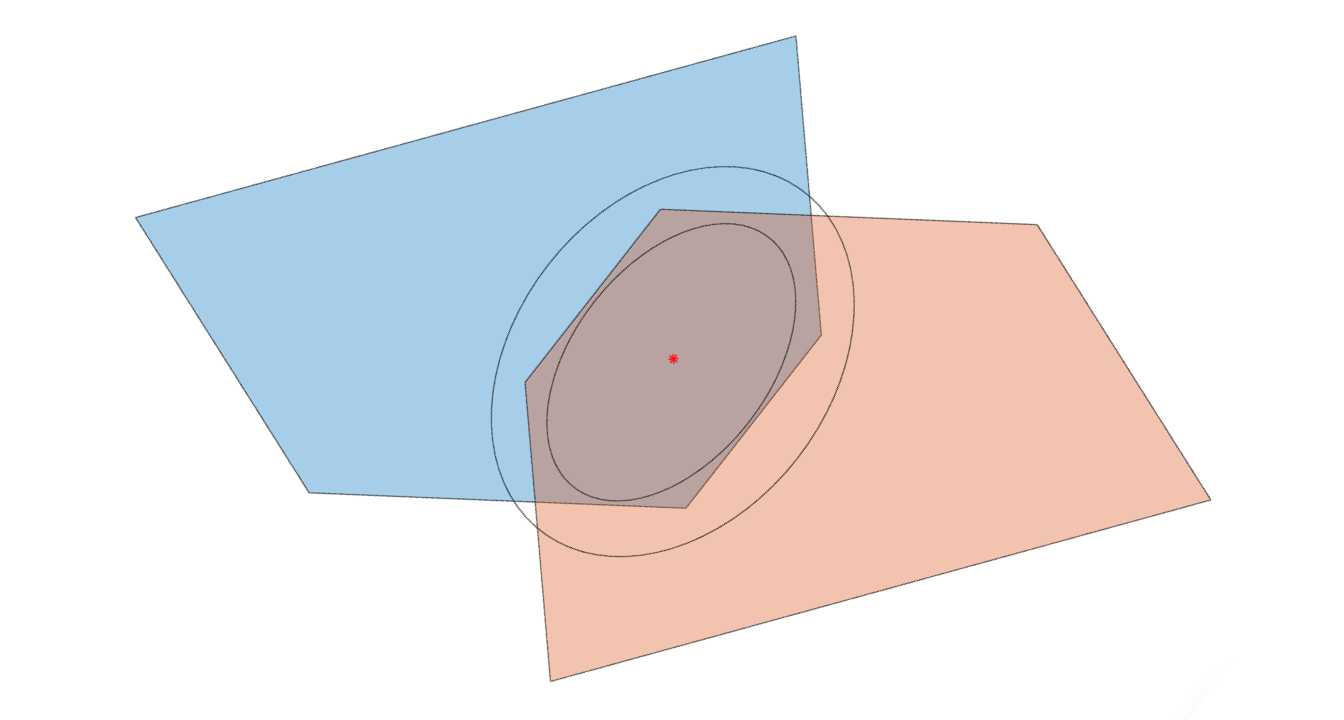
\includegraphics[scale=0.45]{Figures/symmetry}
\par\end{center}%
\end{minipage}\hfill{}%
\begin{minipage}[t]{0.45\textwidth}%
\noindent\begin{flushleft}
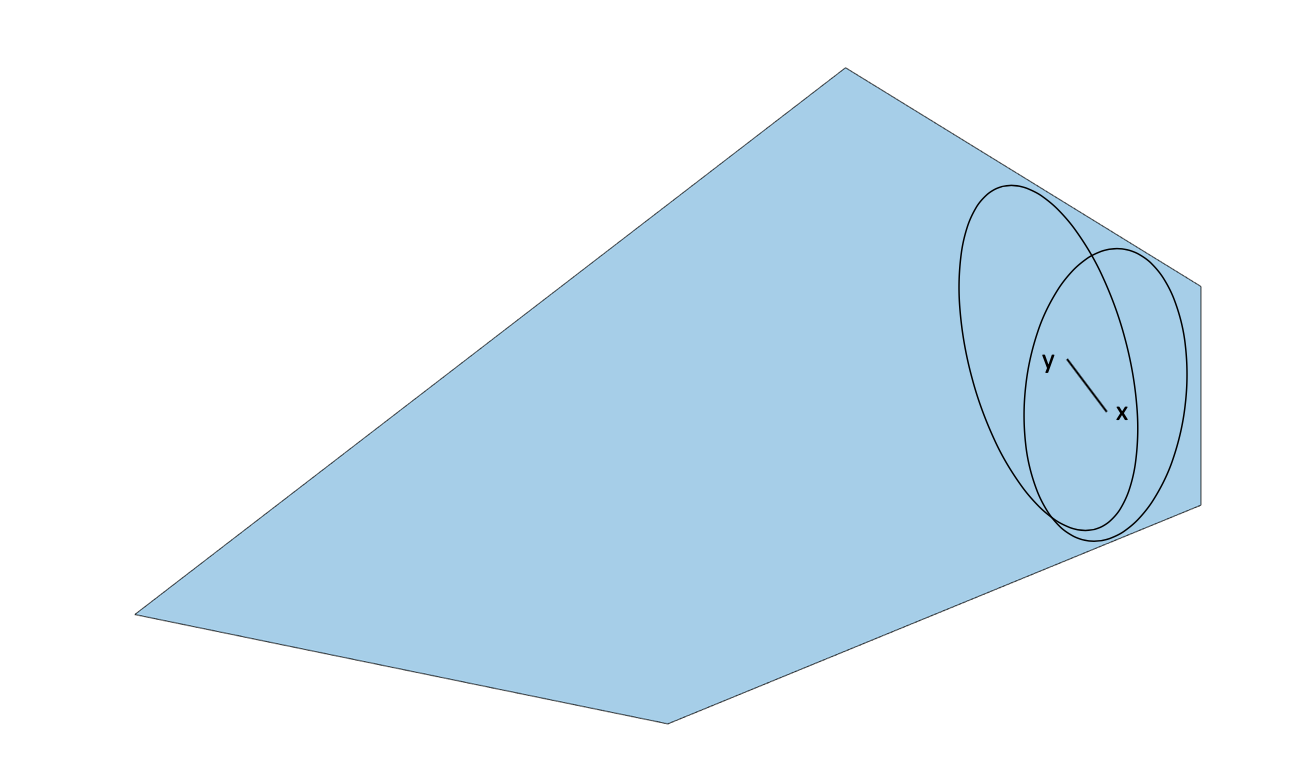
\includegraphics[scale=0.35]{Figures/ssc}
\par\end{flushleft}%
\end{minipage}

\caption{(a) $E_{u}\subseteq K\cap(2u-K)\subseteq\alpha E_{u}.$ (b) Strong
self-concordance measures the rate of change of the Hessian of a barrier
in the Frobenius norm}
\end{figure}
\end{defn}

Similar to Lemma \ref{lem:global_self_concordant}, we have a longer-range
version of stability of the Hessian.
\begin{lem}
\label{lem:global_strongly_self_concordant}Given any strongly self-concordant
matrix function $\mh$ on $K\subset\Rn$, for any $x,y\in K$ with
$\Vert x-y\Vert_{x}<1$, we have
\[
\|\mh(x)^{-\frac{1}{2}}(\mh(y)-\mh(x))\mh(x)^{-\frac{1}{2}}\|_{F}\leq\frac{\|x-y\|_{x}}{(1-\|x-y\|_{x})^{2}}.
\]
\end{lem}

\begin{proof}
Let $x_{t}=(1-t)x+ty$. Then, we have
\begin{align*}
\|\mh(x)^{-\frac{1}{2}}(\mh(y)-\mh(x))\mh(x)^{-\frac{1}{2}}\|_{F} & =\int^{1}_{0}\|\mh(x)^{-\frac{1}{2}}\frac{d}{dt}\mh(x_{t})\mh(x)^{-\frac{1}{2}}\|_{F}dt.
\end{align*}

We note that $\mh$ is self-concordant. Hence, Lemma \ref{lem:global_self_concordant}
shows that
\begin{align*}
\|\mh(x)^{-\frac{1}{2}}\frac{d}{dt}\mh(x_{t})\mh(x)^{-\frac{1}{2}}\|^{2}_{F} & =\tr\mh(x)^{-1}\left(\frac{d}{dt}\mh(x_{t})\right)\mh(x)^{-1}\left(\frac{d}{dt}\mh(x_{t})\right)\\
 & \leq\frac{1}{\left(1-\Vert x-x_{t}\Vert_{x}\right)^{4}}\tr\mh(x_{t})^{-1}\left(\frac{d}{dt}\mh(x_{t})\right)\mh(x_{t})^{-1}\left(\frac{d}{dt}\mh(x_{t})\right)\\
 & \leq\frac{4}{\left(1-\Vert x-x_{t}\Vert_{x}\right)^{4}}\|x-x_{t}\|^{2}_{x_{t}}\\
 & \leq\frac{4}{\left(1-\Vert x-x_{t}\Vert_{x}\right)^{6}}\|x-x_{t}\|^{2}_{x}
\end{align*}

where we used the assumption in the second inequality and Lemma \ref{lem:global_self_concordant}
again for the last inequality. Hence, 
\begin{align*}
\|\mh(x)^{-\frac{1}{2}}(\mh(y)-\mh(x))\mh(x)^{-\frac{1}{2}}\|_{F} & \leq\int^{1}_{0}\frac{2\|x-x_{t}\|_{x}}{\left(1-\Vert x-x_{t}\Vert_{x}\right)^{3}}dt\\
 & =\int^{1}_{0}\frac{2t\|x-y\|_{x}}{(1-t\|x-y\|_{x})^{3}}dt\\
 & =\frac{\|x-y\|_{x}}{(1-\|x-y\|_{x})^{2}}.
\end{align*}
\end{proof}
We note that strong self-concordance can be stronger than self-concordance
since the Frobenius norm is always greater than or equal to the spectral
norm. 
\begin{xca}
Verify that the Hessian of the standard log barrier is strongly self-concordant.
\end{xca}

The main theorem of this section is the following guarantee for the
Dikin walk.
\begin{thm}
\label{thm:dikin}The mixing rate of the Dikin walk with the logarithmic
barrier for a polytope $\{\mathbf{A}x\ge b\}$ is $O(mn)$.
\end{thm}

Each step of the standard Dikin walk can be implemented without using
matrix multiplication.
\begin{thm}
\label{thm:dikin-fast}The Dikin walk with the logarithmic barrier
for a polytope $\{\mathbf{A}x\ge b\}$ can be implemented in time
$O(\nnz(\mathbf{A})+n^{2})$ per step while maintaining the mixing
rate of $O(mn)$.
\end{thm}

A key ingredient of the proof of Theorem \ref{thm:dikin} is the following
lemma.
\begin{lem}
\label{lem:dikin-one-step-1}For two points $x,y\in P$, with $\Vert x-y\Vert_{x}\le\frac{r}{10\sqrt{n}}$,
for $r<0.01$, we have $d_{TV}(P_{x},P_{y})\leq\frac{3}{4}$.
\end{lem}

The proof of this lemma needs several properties captured in the next
exercise.
\begin{xca}
Prove the following for the log barrier in the polytope $\{\mathbf{A}x\ge b\}$:
\end{xca}

\begin{itemize}
\item $\ln\det\mh(x)$ is a convex function.
\item $\Pr_{w\sim E_{x}(r)}\left(\norm{w-x}_{x}\le r\left(1-\frac{1}{n}\right)\right)\ge1-c_{0}r$
for some constant $c_{0}$.
\item $\Pr_{w\sim E_{x}(r)}\left(\norm{w-x}_{w}+\norm{w-x}_{2x-w}\le2r\left(1-\frac{1}{n}\right)\vert\norm{w-x}_{x}\le r\left(1-\frac{1}{n}\right)\right)\ge1-c_{1}r$
for some constant $c_{1}$.
\item $\Pr_{w\sim E_{x}(r)}\left(x\in E_{w}(r)\right)\ge0.5-c_{2}r$ for
some constant $c_{2}$.
\end{itemize}
\begin{proof}[Proof of Lemma \ref{lem:dikin-one-step-1}.]
We have to prove two things: first, the rejection probability is
small, second the ellipsoids used by the Dikin walk at $x,y$ have
large overlap. More precisely, we have
\begin{align}
d_{\mathrm{TV}}(P_{x},P_{y}) & \leq\frac{1}{2}\text{rej}_{x}+\frac{1}{2}\text{rej}_{y}+\frac{1}{2}\frac{\vol(P_{x}\backslash P_{y})}{\vol(P_{x})}+\frac{1}{2}\frac{\vol(P_{y}\backslash P_{x})}{\vol(P_{y})}\nonumber \\
 & =\frac{1}{2}\text{rej}_{x}+\frac{1}{2}\text{rej}_{y}+1-\frac{1}{2}\frac{\vol(P_{x}\cap P_{y})}{\vol(P_{x})}-\frac{1}{2}\frac{\vol(P_{x}\cap P_{y})}{\vol(P_{y})}\label{eq:dikin_formula}
\end{align}
where $\text{rej}_{x}$ and $\text{rej}_{y}$ are the rejection probabilities
at $x$ and $y$.

For the rejection probability at $x$, we consider the algorithm that
picks $z$ from $E_{x}(r)$. Let $f(z)=\ln\det\mathbf{H}(z)$. The
acceptance probability of the sample $z$ is
\begin{equation}
\min\left\{ 1,\frac{\vol(E_{x}(r))}{\vol(E_{z}(r))}\right\} =\min\left\{ 1,\sqrt{\frac{\det(\mathbf{H}(z))}{\det(\mathbf{H}(x))}}\right\} .\label{eq:reject_prob_z}
\end{equation}
By the assumption that $f$ is a convex function, we have that
\begin{equation}
\ln\frac{\det(\mathbf{H}(z))}{\det(\mathbf{H}(x))}=f(z)-f(x)\geq\langle\nabla f(x),z-x\rangle.\label{eq:log_det_Hzx}
\end{equation}
To simplify the notation, we assume $\mh(x)=\mi$. Since $z$ is sampled
from unit ball of radius $r$ centered at $x$, we know that 
\[
\P(v^{\top}(z-x)\geq-\epsilon r\|v\|_{2})\geq1-e^{-n\epsilon^{2}/2}.
\]
In particular, with probability at least $0.99$ in $z$, we have
\begin{equation}
\langle\nabla f(x),z-x\rangle\geq-\frac{4r}{\sqrt{n}}\|\nabla f(x)\|_{2}.\label{eq:grad_prob}
\end{equation}
To compute $\|\nabla f(x)\|^{2}_{2}$, it is easier to compute the
directional derivative of $\nabla f$. Note that 
\begin{align}
\|\nabla f(x)\|_{2} & =\max_{\|v\|_{2}=1}\nabla f(x)^{\top}v\nonumber \\
 & =\max_{\|v\|_{2}=1}\tr(\mh(x)^{-1}D\mh(x)[v])\nonumber \\
 & =\max_{\|v\|_{2}=1}\tr\left(\mh(x)^{-\frac{1}{2}}D\mh(x)[v]\mh(x)^{-\frac{1}{2}}\right)\nonumber \\
 & \leq\max_{\|v\|_{2}=1}\sqrt{n}\|\mh(x)^{-\frac{1}{2}}D\mh(x)[v]\mh(x)^{-\frac{1}{2}}\|_{F}\nonumber \\
 & \leq\sqrt{n}\label{eq:grad_log_H}
\end{align}
where the first inequality follows from $\left|\sum^{n}_{i=1}\lambda_{i}\right|\leq\sqrt{n}\sqrt{\sum^{n}_{i=1}\lambda^{2}_{i}}$
and the second inequality follows from the definition of strong self-concordance.

Combining (\ref{eq:reject_prob_z}), (\ref{eq:log_det_Hzx}), (\ref{eq:grad_prob})
and (\ref{eq:grad_log_H}), we see that with probability at least
$0.99$ in $z$, acceptance probability of the sample $z$, assuming
that $x\in E_{z}(r)$ is 
\begin{equation}
\min\left\{ 1,\frac{\vol(E_{x}(r))}{\vol(E_{z}(r))}\right\} \geq e^{-2r}\geq0.9\label{eq:rejection}
\end{equation}
where we used that $r\le\frac{1}{20}$. Hence the rejection probability
$\mathrm{rej}_{x}$ (and similarly $\mathrm{rej}_{y}$) including
the event $x\in E_{z}(r)$ which happens with probability at least
$0.4$ from the previous exercise, satisfies
\begin{equation}
\mathrm{rej}_{x}\leq0.7\qquad\text{and}\qquad\mathrm{rej}_{y}\leq0.7.\label{eq:rej_xy}
\end{equation}

Now, we bound the fraction of volume in the intersection of the ellipsoids
at $x,y$. Again, we can assume that $\mh(x)=\mi$. Then, strong self-concordance
and Lemma \ref{lem:global_strongly_self_concordant} shows that
\begin{equation}
\|\mh(y)-\mi\|_{F}\leq2\|x-y\|_{x}\leq\frac{1}{10\sqrt{n}}.\label{eq:H_minus_I_F}
\end{equation}
In particular, we have that 
\begin{equation}
0.9\mi\preceq\mh(y)\preceq1.1\mi.\label{eq:H_I_op}
\end{equation}

We partition the eigenvalues $\lambda_{i}$ of $\mh(y)$ into those
of value at least $1$ and the rest. Then consider the ellipsoid $E$
whose eigenvalues are $\min\left\{ 1,\lambda_{i}\right\} $. This
is contained in both $E_{x}(1)$ and $E_{y}(1)$. We will see that
$\vol(E)$ is a constant fraction of the volume of both $E_{x}(1)$
and $E_{y}(1)$. First, we compare $E$ and $E_{x}(1)$
\begin{equation}
\frac{\vol(E)}{\vol(E_{x}(1))}=\prod_{i:\lambda_{i}<1}\lambda_{i}=\prod_{i:\lambda_{i}<1}\left(1-(1-\lambda_{i})\right)\geq\exp\left(-2\sum_{i:\lambda_{i}<1}\left(1-\lambda_{i}\right)\right)\label{eq:vol_E_x}
\end{equation}
where we used that $1-x\geq\exp(-2x)$ for $0\leq x\leq\frac{1}{2}$
and $\lambda_{i}\geq\frac{1}{2}$ (\ref{eq:H_I_op}). From the inequality
(\ref{eq:H_minus_I_F}), it follows that
\[
\sqrt{\sum_{i}(\lambda_{i}-1)^{2}}\le\frac{1}{10\sqrt{n}}.
\]
Therefore, $\sum_{i:\lambda_{i}<1}|\lambda_{i}-1|\leq0.1$. Putting
it into (\ref{eq:vol_E_x}), we have
\begin{equation}
\frac{\vol(P_{x}\cap P_{y})}{\vol(P_{x})}=\frac{\vol(E)}{\vol(E_{x}(1))}\geq e^{-0.2}.\label{eq:volPxyPx}
\end{equation}
Similarly, we have
\begin{equation}
\frac{\vol(P_{x}\cap P_{y})}{\vol(P_{y})}=\frac{\prod_{i:\lambda_{i}<1}\lambda_{i}}{\prod_{i:\lambda_{i}}\lambda_{i}}=\frac{1}{\prod_{i:\lambda_{i}>1}\lambda_{i}}\geq\frac{1}{\exp(\sum_{i:\lambda_{i}>1}(\lambda_{i}-1))}\geq e^{-0.1}.\label{eq:volPxyPy}
\end{equation}

Putting (\ref{eq:rej_xy}), (\ref{eq:volPxyPx}) and (\ref{eq:volPxyPy})
into (\ref{eq:dikin_formula}), we have
\[
d_{\mathrm{TV}}(P_{x},P_{y})\leq\frac{0.7}{2}+\frac{0.7}{2}+1-\frac{e^{-0.2}}{2}-\frac{e^{-0.1}}{2}\leq\frac{3}{4}.
\]
\end{proof}
The other key ingredient for proving the mixing rate is an isoperimetric
inequality. We will in fact use the one for the cross-ratio distance
(Theorem \ref{thm:iso-cross-ratio}) that came up in the analysis
of Hit-and-Run. We can relate the cross-ratio distance to the local
norm induced by the Dikin ellipsoid.
\begin{lem}
\label{lem:dikin-dist-1}For $u,v\in K$, $d_{K}(u,v)\ge\frac{\Vert u-v\Vert_{u}}{\sqrt{m}}$
where $\norm{\cdot}_{u}$ is the norm induced by the Hessian of the
log barrier. 
\end{lem}

The proof will need the following elementary fact about the log barrier.
\begin{lem}
\label{lem:dikin_sandwich}For the Dikin ellipsoid induced by any
self-concordant barrier, we have $E_{x}(1)\subseteq K\cap(2x-K)$
and for the logarithmic barrier for a polytope $K=\{\mathbf{A}x\ge b\}$
defined by $m$ inequalities we also have $K\cap(2x-K)\subseteq E_{x}(\sqrt{m})$.
\end{lem}

\begin{proof}
For the first inequality, we notice that since for any $x\in K$,
we have that the barrier function $\phi$ is finite with bounded first
and second derivatives, and by Lemma \ref{lem:global_self_concordant},
the Hessian remains finite for every point in $[x,y]$ for $y$ such
that $\norm{x-y}_{x}<1$, we have that $\phi(y)$ is also finite,
and hence $y\in K$, since $\phi$ is a barrier function for $K$. 

For the second part, for any $y\in K\cap(2x-K)$, we have that for
every $i\in[m]$, 
\[
\left|a^{\top}_{i}y-a^{\top}_{i}x\right|\le a^{\top}_{i}x-b_{i}
\]
and hence 
\[
\frac{\left|a^{\top}_{i}y-a^{\top}_{i}x\right|}{a^{\top}_{i}x-b_{i}}\le1.
\]
Therefore, 
\[
(y-x)^{\top}\nabla^{2}\phi(x)(y-x)=\sum^{m}_{i=1}\frac{\left(a^{\top}_{i}(y-x)\right)^{2}}{\left(a^{\top}_{i}x-b_{i}\right)^{2}}\le m.
\]
\end{proof}
We can now prove Lemma \ref{lem:dikin-dist-1}.
\begin{proof}[Proof of Lemma \ref{lem:dikin-dist-1}.]
 Consider the ellipsoid at $u$. For the chord $[p,q]$ induced by
$u,v$ with these points in the order $p,u,v,q$, suppose that $\|p-u\|_{2}\le\|v-q\|_{2}$.
Then by Lemma \ref{lem:dikin_sandwich}, $p\in K\cap(2u-K)$. And
hence $\|p-u\|_{u}\le\sqrt{m}.$ Therefore, 
\[
d_{K}(u,v)=\frac{\|u-v\|_{2}\|p-q\|_{2}}{\|p-u\|_{2}\|v-q\|_{2}}\geq\frac{\|u-v\|_{2}}{\|p-u\|_{2}}=\frac{\|u-v\|_{u}}{\|p-u\|_{u}}\ge\frac{\|u-v\|_{u}}{\sqrt{m}}.
\]
\end{proof}
We can now prove the main conductance bound.
\begin{thm}
The conductance of the Dikin walk with the log barrier applied to
a polytope $\{\mathbf{A}x\ge b\}$ with any $r<0.01$ is $\Omega(r/\sqrt{mn})$.
\end{thm}

\begin{proof}
We follow the standard high-level outline. Consider any measurable
subset $S_{1}\subseteq K$ and let $S_{2}=K\setminus S_{1}$ be its
complement. Define the points with low escape probability for these
subsets as:
\[
S_{i}'=\left\{ x\in S_{i}:\,P_{x}(K\setminus S_{i})<\frac{1}{8}\right\} 
\]
and let $S_{3}'=K\setminus S_{1}'\setminus S_{2}'$. Then, for any
$u\in S_{1}'$, $v\in S_{2}'$, we have $d_{TV}(P_{u},P_{v})>1-\frac{1}{4}$.
Hence, by Lemma \ref{lem:dikin-one-step-1}, we have $\Vert u-v\Vert_{u}\ge\frac{r}{10\sqrt{n}}$.
Therefore, by Lemma \ref{lem:dikin-dist-1}, 
\[
d_{K}(u,v)\ge\frac{r}{10\sqrt{n}\cdot\sqrt{m}}.
\]
We can now bound the conductance of $S_{1}$. We may assume that $\vol(S_{i}')\ge\vol(S_{i})/2$;
otherwise, it immediately follows that the conductance of $S_{1}$
is $\Omega(1)$. Assuming this, we have
\begin{align*}
\int_{S_{1}}P_{x}(S_{2})\,dx & \ge\frac{1}{2}\int_{S_{3}'}\frac{1}{8}dx\ge\frac{1}{16}\vol(S_{3}')\\
 & \ge\frac{1}{16}d_{K}(S_{1}',S_{2}')\frac{\vol(S_{1}')\vol(S_{2}')}{\vol(P)}\qquad\text{(Theorem \ref{thm:iso-cross-ratio})}\\
 & \ge\frac{r}{1000\sqrt{nm}}\min\left\{ \vol(S_{1}),\vol(S_{2})\right\} .
\end{align*}
\end{proof}


\section{Hamiltonian Monte Carlo}

Hamiltonian dynamics is an alternative way to formulate Newtonian
mechanics. The Hamiltonian $H$ captures both the potential and kinetic
energy of a particle as a function of its position and velocity. The
dynamics can be described by the following differential equations.
\begin{align*}
\frac{dx}{dt} & =\frac{\partial H(x,v)}{\partial v},\\
\frac{dv}{dt} & =-\frac{\partial H(x,v)}{\partial x}.
\end{align*}
These equations preserve the Hamiltonian function $H$. In the simplest
Euclidean setting, it can be defined as follows.
\[
H(x,v)=f(x)+\frac{1}{2}\norm v^{2}
\]
so that 
\[
\frac{dx}{dt}=v,\quad\frac{dv}{dt}=-\nabla f(x)
\]
or
\[
\frac{d^{2}x}{dt^{2}}=-\nabla f(x).
\]

More generally, the Hamiltonian can depend on a function that defines
a local metric:
\[
H(x,v)=f(x)+\frac{1}{2}\log((2\pi)^{n}\det g(x))+\frac{1}{2}v^{T}g(x)^{-1}v
\]
where $g(x)$ is a matrix, and when it is positive definite, it defines
a local norm at $x$. In this sense, we can view the dynamics as evolving
on a manifold with local metric $g(x)$. Here in this chapter, we
will focus on the case when $g(x)=I$, the standard Euclidean metric.

(Riemannian) Hamiltonian Monte Carlo (or RHMC) \cite{Neal1996,Neal2012}\cite{Girolami2009,Girolami2011}
is a Markov chain Monte Carlo method for sampling from a desired distribution.
Each step of the method consists of the following: At a current point
$x$,
\begin{enumerate}
\item Pick a random velocity $y$ according to a local distribution defined
by $x$ (in the simplest setting, this is the standard Gaussian distribution
for every $x$).
\item Move along the Hamiltonian curve defined by Hamiltonian dynamics at
$(x,y)$ for time (distance) $\delta$.
\end{enumerate}
For the choice of $H$ above, the marginal distribution of the current
point $x$ approaches the target distribution with density proportional
to $e^{-f}$. For the exact Hamiltonian flow $T_{\step}$, no Metropolis
correction is needed.In numerical HMC, an inexact reversible volume-preserving
integrator is usually paired with a Metropolis filter to correct discretization
error. For exact flow, there is no discretization step size to tune.
For numerical integrators, the integrator step size is still constrained
by accuracy and acceptance probability, even though the Metropolis
filter corrects the stationary distribution. Hamiltonian Monte Carlo
can be used for sampling from a general distribution $e^{-H(x,y)}$. 
\begin{defn}
Given a continuous, twice-differentiable function $H:\mathcal{M}\times\Rn\subset\R^{n}\times\R^{n}\rightarrow\R$
(\emph{Hamiltonian}) where $\mathcal{M}$ is the domain of the $x$-coordinate
of $H$, we say $(x(t),y(t))$ follows a \emph{Hamiltonian curve}
if it satisfies the \emph{Hamiltonian equations}

\begin{align}
\frac{dx}{dt} & =\frac{\partial H(x,y)}{\partial y},\nonumber \\
\frac{dy}{dt} & =-\frac{\partial H(x,y)}{\partial x}.\label{eq:ham}
\end{align}
We define the map $T_{\step}(x,y)\defeq(x(\step),y(\step))$ where
$(x(t),y(t))$ follows the Hamiltonian curve with the initial condition
$(x(0),y(0))=(x,y).$
\end{defn}

Hamiltonian Monte Carlo is a Markov chain generated by a sequence
of random Hamiltonian curves.

\begin{algorithm2e}

\caption{Hamiltonian Monte Carlo}

\SetAlgoLined

\textbf{Input:} some initial point $x^{(1)}\in\mathcal{M}$.

\For{$k=1,2,\cdots,T$}{

Sample $y$ according to $e^{-H(x^{(k)},y)}/\pi(x^{(k)})$ where $\pi(x)=\int_{\Rn}e^{-H(x,y)}dy$.

With probability $\frac{1}{2}$, set $(x^{(k+1)},y^{(k+1)})=T_{\step}(x^{(k)},y)$. 

Otherwise, $(x^{(k+1)},y^{(k+1)})=T_{-\step}(x^{(k)},y)$.

}

\textbf{Output:} $(x^{(T+1)},y^{(T+1)})$.

\end{algorithm2e}

\subsection*{Time-reversibility }
\begin{lem}[Energy Conservation]
\label{lem:ham_eng_pre}For any Hamiltonian curve $(x(t),y(t))$,
we have that
\[
\frac{d}{dt}H(x(t),y(t))=0.
\]
\end{lem}

\begin{proof}
Note that
\[
\frac{d}{dt}H(x(t),y(t))=\frac{\partial H}{\partial x}\frac{dx}{dt}+\frac{\partial H}{\partial y}\frac{dy}{dt}=\frac{\partial H}{\partial x}\frac{\partial H}{\partial y}-\frac{\partial H}{\partial y}\frac{\partial H}{\partial x}=0.
\]
\end{proof}
\begin{lem}[Measure Preservation]
\label{lem:ham_measure_pre}For any $t\geq0$, we have that
\[
\det\left(DT_{t}(x,y)\right)=1
\]
where $DT_{t}(x,y)$ is the Jacobian of the map $T_{t}$ at the point
$(x,y)$.
\end{lem}

\begin{proof}
Let $(x(t,s),y(t,s))$ be a family of Hamiltonian curves given by
$T_{t}(x+sd_{x},y+sd_{y})$. We write 
\[
u(t)=\frac{\partial}{\partial s}x(t,s)|_{s=0}\,,\,v(t)=\frac{\partial}{\partial s}y(t,s)|_{s=0}.
\]
By differentiating the Hamiltonian equations (\ref{eq:ham}) with
respect to $s$, we have that
\begin{align*}
\frac{du}{dt} & =\frac{\partial^{2}H(x,y)}{\partial y\partial x}u+\frac{\partial^{2}H(x,y)}{\partial y\partial y}v,\\
\frac{dv}{dt} & =-\frac{\partial^{2}H(x,y)}{\partial x\partial x}u-\frac{\partial^{2}H(x,y)}{\partial x\partial y}v,\\
(u(0),v(0)) & =(d_{x},d_{y}).
\end{align*}
This can be captured by the following matrix ODE
\begin{align*}
\frac{d\Phi}{dt} & =\left(\begin{array}{cc}
\frac{\partial^{2}H(x(t),y(t))}{\partial y\partial x} & \frac{\partial^{2}H(x(t),y(t))}{\partial y\partial y}\\
-\frac{\partial^{2}H(x(t),y(t))}{\partial x\partial x} & -\frac{\partial^{2}H(x(t),y(t))}{\partial x\partial y}
\end{array}\right)\Phi(t)\\
\Phi(0) & =I
\end{align*}
using the equation
\[
DT_{t}(x,y)\left(\begin{array}{c}
d_{x}\\
d_{y}
\end{array}\right)=\left(\begin{array}{c}
u(t)\\
v(t)
\end{array}\right)=\Phi(t)\left(\begin{array}{c}
d_{x}\\
d_{y}
\end{array}\right).
\]
Therefore, $DT_{t}(x,y)=\Phi(t)$. Next, we observe that
\[
\frac{d}{dt}\log\det\Phi(t)=\tr\left(\Phi(t)^{-1}\frac{d}{dt}\Phi(t)\right)=\tr\left(\begin{array}{cc}
\frac{\partial^{2}H(x(t),y(t))}{\partial y\partial x} & \frac{\partial^{2}H(x(t),y(t))}{\partial y\partial y}\\
-\frac{\partial^{2}H(x(t),y(t))}{\partial x\partial x} & -\frac{\partial^{2}H(x(t),y(t))}{\partial x\partial y}
\end{array}\right)=0.
\]
Hence,
\[
\det\Phi(t)=\det\Phi(0)=1.
\]
\end{proof}
Using the previous two lemmas, we can see that Hamiltonian Monte Carlo
indeed converges to the desired distribution. 
\begin{lem}[Time reversibility]
\label{lem:time_reversibility}Let $p_{x}(x')$ denote the probability
density of one step of the Hamiltonian Monte Carlo starting at $x$.
We have that\textup{
\[
\pi(x)p_{x}(x')=\pi(x')p_{x'}(x)
\]
for almost every $x$ and $x'$ where $\pi(x)=\int_{\Rn}e^{-H(x,y)}dy$.}
\end{lem}

\begin{proof}
Fix $x$ and $x'$. Let $F^{x}_{\step}(y)$ be the $x$ component
of $T_{\step}(x,y)$. Let $V_{+}=\{y:\text{ }F^{x}_{\step}(y)=x'\}$
and $V_{-}=\{y:\text{ }F^{x}_{-\step}(y)=x'\}$. Then, 
\[
\pi(x)p_{x}(x')=\frac{1}{2}\int_{y\in V_{+}}\frac{e^{-H(x,y)}}{\left|\det\left(DF^{x}_{\step}(y)\right)\right|}+\frac{1}{2}\int_{y\in V_{-}}\frac{e^{-H(x,y)}}{\left|\det\left(DF^{x}_{-\step}(y)\right)\right|}.
\]
We note that this formula assumes that $DF^{x}_{\step}$ is invertible.
Sard's theorem shows that $F^{x}_{\step}(N)$ has measure $0$ where
$N\defeq\{y:\,DF^{x}_{\step}(y)\text{ is not invertible}\}$. The
same argument applies to $F^{x}_{-\step}$. Therefore, the formula
is correct except for a measure zero subset of target points.

By reversing time for the Hamiltonian curve, we have that for the
same $V_{\pm}$, 
\begin{equation}
\pi(x')p_{x'}(x)=\frac{1}{2}\int_{y\in V_{+}}\frac{e^{-H(x',y')}}{\left|\det\left(DF^{x'}_{-\step}(y')\right)\right|}+\frac{1}{2}\int_{y\in V_{-}}\frac{e^{-H(x',y')}}{\left|\det\left(DF^{x'}_{\step}(y')\right)\right|}\label{eq:ham_transit}
\end{equation}
where $y'$ denotes the $y$ component of $T_{\step}(x,y)$ and $T_{-\step}(x,y)$
in the first and second terms, respectively.

We compare the first terms in both equations. Let $DT_{\step}(x,y)=\left(\begin{array}{cc}
A & B\\
C & D
\end{array}\right)$. At the regular points used in the change-of-variables formula, the
block$B=DF^{x}_{\step}(y)$ is invertible. Let $DT_{-\step}(x',y')=\left(\begin{array}{cc}
* & M\\*
 & *
\end{array}\right)$. Then $M=DF^{x'}_{-\step}(y')$. Since $T_{-\step}$ is the inverse
of $T_{\step}$, this matrix is the inverse of $DT_{\step}(x,y)$.
To compute $M$, solve $\left(\begin{array}{cc}
A & B\\
C & D
\end{array}\right)\binom{u}{v}=\binom{0}{q}$. The first block equation gives $v=-B^{-1}Au$, and the second gives
$(C-DB^{-1}A)u=q$. Thus $M=(C-DB^{-1}A)^{-1}$. Therefore, we have
that $DF^{x}_{\step}(y)=B$ and $DF^{x'}_{-\step}(y')=(C-DB^{-1}A)^{-1}$.
Hence, we have that
\begin{align*}
\left|\det\left(DF^{x'}_{-\step}(y')\right)\right| & =\left|\det(C-DB^{-1}A)^{-1}\right|=\frac{\left|\det B\right|}{\left|\det\left(\begin{array}{cc}
A & B\\
C & D
\end{array}\right)\right|}.
\end{align*}
Using that $\det\left(DT_{t}(x,y)\right)=\det\left(\begin{array}{cc}
A & B\\
C & D
\end{array}\right)=1$ (Lemma \ref{lem:ham_measure_pre}), we have that
\[
\left|\det\left(DF^{x'}_{-\step}(y')\right)\right|=\left|\det\left(DF^{x}_{\step}(y)\right)\right|.
\]
Hence, we have that
\begin{align*}
\frac{1}{2}\int_{y\in V_{+}}\frac{e^{-H(x,y)}}{\left|\det\left(DF^{x}_{\step}(y)\right)\right|} & =\frac{1}{2}\int_{y\in V_{+}}\frac{e^{-H(x,y)}}{\left|\det\left(DF^{x'}_{-\step}(y')\right)\right|}\\
 & =\frac{1}{2}\int_{y\in V_{+}}\frac{e^{-H(x',y')}}{\left|\det\left(DF^{x'}_{-\step}(y')\right)\right|}
\end{align*}
where we used that $e^{-H(x,y)}=e^{-H(x',y')}$ (Lemma \ref{lem:ham_eng_pre})
at the end. 

For the second term in (\ref{eq:ham_transit}), by the same calculation,
we have that
\[
\frac{1}{2}\int_{y\in V_{-}}\frac{e^{-H(x,y)}}{\left|\det\left(DF^{x}_{-\step}(y)\right)\right|}=\frac{1}{2}\int_{y\in V_{-}}\frac{e^{-H(x',y')}}{\left|\det\left(DF^{x'}_{\step}(y')\right)\right|}
\]
\end{proof}

\subsection*{Convergence}

First, we consider convergence when $H(x,v)=f(x)+\frac{1}{2}\norm v^{2}$
for a strongly convex function $f$. So the marginal of the stationary
distribution along $x$ is proportional to $e^{-f}$. The idea here
is coupling (as we did for Langevin dynamics). We consider two separate
processes $x$ and $y$, with their next step directions chosen to
be identical. The key lemma is that under this coupling the squared
distance decreases up to a certain time that depends on the condition
number. For a tight analysis, showing a mixing rate of $O(\kappa)$
where the condition number $\kappa$ is the ratio of the Lipschitz
constant of the gradient of $f$ to its strong convexity parameter,
we refer the reader to \cite{chen2022optimal}. The general Riemannian
setting, which gives an affine-invariant sampling algorithm, was analyzed
in \cite{LV2022geodesic,LV18riemannian}, showing that when applied
to polytopes with the Lewis weights barrier, the resulting process
converges with a mixing rate of $\tilde{O}(mn^{2/3})$ and each iteration
has time complexity $O(mn^{\omega-1})$. 


\chapter{Annealing \label{chap:Annealing} }


\paragraph*{Integration and Volume Computation. }

In this chapter, we develop efficient algorithms for volume computation
and integration based on a technique called \emph{Simulated Annealing,
}which is also provably efficient for convex optimization. The volume
problem was defined in Chapter (\ref{chap:Elimination-and-Reduction})
(Problem (\ref{problem:volume})). Integration is the following generalization.
\begin{problem}[Integration]
 Given an evaluation oracle for an integrable logconcave function
$f:\R^{n}\rightarrow\R$, a point $x_{0}$ s.t. $f(x_{0})\ge\beta,$
numbers $r,R>0$ s.t. (i) $\E(\norm{x-x_{0}}^{2})\le R^{2}$ (ii)
the level set of $\pi_{f}$ of measure $1/8$ contains a ball of radius
$r$, and $\varepsilon>0$, output a number $A$ s.t. 
\[
(1-\varepsilon)\int f\le A\le(1+\varepsilon)\int f.
\]

As in all problems in oracle models discussed in this book, the complexity
of an algorithm to solve the above problem is given by the number
of oracles calls and the number of arithmetic operations. 
\end{problem}

Table \ref{tab:volume} below summarizes progress on the volume problem
over the past three decades. Besides improving the complexity of volume
computation, each step has typically resulted in new techniques. For
more details, we refer the reader to surveys on the topic \cite{Simonovits03,VemSurvey}.

\begin{table}[h]
\centering{}%
\begin{tabular}{|c|l|c|}
\hline 
Year/Authors & New ingredients & Steps\tabularnewline
\hline 
\hline 
1989/Dyer-Frieze-Kannan \cite{DyerFK89} & Everything & $n^{23}$\tabularnewline
\hline 
1990/Lov�sz-Simonovits \cite{LS90} & Better isoperimetry & $n^{16}$\tabularnewline
\hline 
1990/Lov�sz \cite{L90} & Ball walk & $n^{10}$\tabularnewline
\hline 
1991/Applegate-Kannan \cite{applegate1991sampling} & Logconcave sampling & $n^{10}$\tabularnewline
\hline 
1990/Dyer-Frieze \cite{DyerF90} & Better error analysis & $n^{8}$\tabularnewline
\hline 
1993/Lov�sz-Simonovits \cite{LS93} & Localization lemma & $n^{7}$\tabularnewline
\hline 
1997/Kannan-Lov�sz-Simonovits \cite{kannan1997random} & Speedy walk, isotropy & $n^{5}$\tabularnewline
\hline 
2003/Lov�sz-Vempala \cite{LV2003} & Annealing, hit-and-run & $n^{4}$\tabularnewline
\hline 
2015/Cousins-Vempala \cite{CV2015} (well-rounded) & Gaussian Cooling & $n^{3}$\tabularnewline
\hline 
2017/Lee-Vempala (polytopes) \cite{lee2017convergence} & Hamiltonian Walk & $mn^{\frac{2}{3}}$\tabularnewline
\hline 
2021/Jia-Laddha-Lee-Vempala \cite{JLLV26} & Faster rounding & $n^{3.5}$\tabularnewline
\hline 
\end{tabular}\caption{\label{tab:volume} The complexity of volume estimation, each step
uses $\widetilde{O}(n)$ bit of randomness. The last algorithm needs
$\widetilde{O}\left(mn^{\omega-1}\right)$ steps per iteration while
the rest need $O(n^{2})$ per oracle query.}
\end{table}
We begin with a description and analysis of the DFK algorithm to estimate
the volume of a convex body in high dimension.

\section{Volume Computation: the DFK Algorithm}
\begin{thm}
There exists a randomized algorithm that given any $\varepsilon,\delta>0$,
and any convex body $K$ with probability at least $1-\delta$ solves
the Volume Estimation problem for $K$ using $\mbox{poly}(n,1/\varepsilon,\ln(1/\delta),\ln R)$
oracle queries and arithmetic operations. 
\end{thm}

The next exercise is the general observation that any algorithm that
succeeds with failure probability less than $1/2$ can be converted
to one with failure probability at most $\delta$. 
\begin{xca}
Show that a randomized algorithm that outputs an acceptable estimate
of a real number with failure probability at most $1/4$ can be converted
to one that outputs an acceptable estimate with failure probability
at most $\delta$ by repeating the algorithm independently $O(\ln(1/\delta))$
times and taking the median of the outputs of the independent trials.

Going forward, we ignore the parameter $\delta$, and focus on algorithms
with constant failure probability. We will now show an algorithm for
volume computation (as a first attempt) whose analysis yields a suboptimal
bound on the sample complexity.

The polynomial-time algorithm of Dyer, Frieze and Kannan \cite{DyerFK89}
is based on the following idea. We consider a sequence of convex bodies
$K_{0}=B_{n}\subset K_{1}\subseteq\ldots\subseteq K_{m}=K$, starting
with the ball contained inside the input body $K$ and ending with
$K$ itself. Then the following telescoping formula suggests an algorithm:
\[
\vol(K)=\vol(K_{0})\cdot\frac{\vol(K_{1})}{\vol(K_{0})}\cdot\ldots\cdot\frac{\vol(K_{m})}{\vol(K_{m-1})}.
\]

To estimate the volume of $K$, we estimate each of the ratios on
the RHS and output their product together with the volume of the unit
ball. We need to set up the sequence so that the sequence is not too
long and this estimator is accurate and efficient. In the DFK algorithm,
each body in the sequence is a ball intersected with the given convex
body $K$:
\[
K_{i}=2^{\frac{i}{n}}B\cap K.
\]
 The length the sequence is $m=\lceil n\log R\rceil$ so that the
final body is just $K$. We can now state the algorithm. In each iteration
the algorithm estimates the ratio $\vol(K_{i})/\vol(K_{i+1})$ by
sampling uniformly from $K_{i+1}$ and using the fraction of the sample
that lies in $K_{i}$ as the estimator.
\end{xca}

\begin{algorithm2e}[H]

\caption{$\mathtt{DFK\ Volume}$}

\SetAlgoLined
\begin{enumerate}
\item For $i=0,\ldots,m=\lceil n\log_{2}R\rceil$, let $K_{i}=2^{\frac{i}{n}}B\cap K.$
\item For $i=0,\ldots,m-1$, 
\begin{enumerate}
\item uniformly sample $X^{(1)},X^{(2)},\ldots,X^{(N)}$ from $K_{i+1}$.
\item Set $Y_{i}=|{\{j:X^{(j)}\in K_{i}\}}|/N$. 
\end{enumerate}
\item Let $Y=\prod_{i=1}^{m-1}Y_{i}$ and return $\vol(B_{n})/Y$.
\end{enumerate}
\end{algorithm2e}

The following observation is immediate.
\begin{lem}
Let $r_{i}=\vol(K_{i})/\vol(K_{i+1})$. Then $\E(Y_{i})=r_{i}$ and
$\Var(Y_{i})=r_{i}(1-r_{i})/N.$
\end{lem}

Since we want to output a multiplicative approximation, we need $\Var(Y)$
to be small compared to $\E(Y)^{2}$, which means we need $r_{i}$
to be bounded from below. The choice of $K_{i}$ is precisely to ensure
this.
\begin{lem}
\label{lem:r_bound}For all $i=0,\ldots,m-1$, we have $\vol(K_{i+1})\le2\vol(K_{i})$. 
\end{lem}

\begin{proof}
We have 
\[
K_{i+1}=2^{(i+1)/n}B_{n}\cap K\subseteq2^{1/n}(2^{i/n}B_{n}\cap K)=2^{1/n}K_{i}.
\]
The lemma follows.
\end{proof}
Using the above lemmas in each phase, and keeping the total error
over $m$ phases smaller than a target $\varepsilon$ leads to a bound
of $N=O(m^{3}/\varepsilon^{2})$ samples per phase. The next lemma
which applies to any product of independent random variables gives
us the ``right'' bound.
\begin{lem}
\label{lem:prod_var}Let $Y=\prod_{i=0}^{m-1}Y_{i}$ where $Y_{i}\ge0$
are independent real-valued random variables. Then, 
\[
\frac{\Var(Y)}{\E(Y)^{2}}=\prod_{i=0}^{m-1}\left(1+\frac{\Var(Y_{i})}{\E(Y_{i})^{2}}\right)-1.
\]
\end{lem}

We can now prove the main theorem about the sample complexity of the
DFK volume algorithm.
\begin{thm}
For any input convex body $K$ satisfying $B_{n}\subseteq K\subseteq RB_{n}$
given by a membership oracle and any $\varepsilon>0$, with $N=O(\varepsilon^{-2}n\log R)$
samples per phase, with probability at least $3/4$, the DFK volume
algorithm outputs a multiplicative $(1+\varepsilon)$ approximation
to the volume of $K$. The total number of samples is thus $O^{*}(m^{2})=O^{*}(n^{2})$. 
\end{thm}

\begin{proof}
In each phase we have 
\[
\frac{\Var(Y_{i})}{\E(Y_{i})^{2}}=\frac{r_{i}(1-r_{i})}{Nr_{i}^{2}}=\frac{1-r_{i}}{Nr_{i}}\le\frac{1}{N}
\]
where we used the fact that $r_{i}\ge1/2$ from Lemma \ref{lem:r_bound}.
Now using Lemma \ref{lem:prod_var}, we have 
\[
\frac{\Var(Y)}{\E(Y)^{2}}\le\left(1+\frac{1}{N}\right)^{m}-1\le\frac{\varepsilon^{2}}{4}
\]
where we used that $(1+\frac{1}{N})^{m}-1\leq\frac{2m}{N}$ for $N\ge8m/\varepsilon^{2}$.
The theorem follows using Chebyshev's inequality.
\end{proof}
In \cite{kannan1997random}, it was shown that the amortized complexity
of uniform sampling is $O^{*}(n^{3})$ per sample when $\Omega(n^{2})$
samples are needed, giving an overall oracle complexity of $O^{*}(n^{5})$
for the entire algorithm. To make this rigorous, besides establishing
the amortized complexity of uniform sampling, we have to deal with
some nontrivial technical issues: (1) the distribution from which
samples are produced is close to the target uniform distribution but
not exactly uniform (2) samples are nearly independent but not perfectly
independent. Another important problem that will arise in establishing
the complexity of (approximate) uniform sampling is ``rounding''
which allows us to reduce the dependence of the sampling complexity
from polynomial in $R$ to polynomial in $\log R$. 

The quadratic sample complexity might appear to be nearly optimal
-- the final ratio being estimated could be as large as $R^{n}$
or $n^{n}$, which means that any sequence that uses at most $m$
phases estimates a ratio as large as $n^{n/m}$ needing as many samples,
and this means that $m=\Omega(n)$ is needed to get polynomial complexity
even. We will soon see that this intuitive reasoning is not valid. 

\section{Simulated Annealing}

In this section we introduce a sampling-based approach for optimization
and integration in high dimension. The main idea is to sample a sequence
of logconcave distributions, starting with one that is easy to integrate
and ending with the function whose integral is desired. This process
is known as \emph{simulated annealing. }The same high-level algorithm
can be used for optimization, volume computation/integration or rounding.
For integration, the desired integral of a function $f:\R^{n}\rightarrow\R_{+}$
can be expressed as the following telescoping product:

\[
\int_{\R^{n}}f=\int f_{0}\frac{\int f_{1}}{\int f_{0}}\frac{\int f_{2}}{\int f_{3}}\cdots\frac{\int f_{m}}{\int f_{m-1}}
\]
where $f_{0}$ is chosen to be a function with an easy integral (typically
a formula) and $f_{m}=f$. To compute any the ratio $\int g/\int h$
we can do the following: 
\begin{enumerate}
\item Sample $X$ from the distribution with density proportional to $h$. 
\item Use the estimator $Y=\frac{g(X)}{h(X)}$. 
\end{enumerate}
It is easy to establish the following fact about this estimator. 
\begin{lem}
For integrable functions $g,h$ with with support of $g$ contained
in the support of $h$ and $g(X)/h(X)$ defined everywhere in the
support of $h$, for $X$ drawn from the distribution with density
proportional to $h$ and $Y=g(X)/h(X)$, we have 
\[
\E(Y)=\frac{\int g}{\int h}.
\]
 
\end{lem}

Of course, the accuracy of the estimator depends on its variance.
Our goal is to choose a sequence of functions that are easy to sample
and lead to a small variance estimator. What sequence of functions
should we use?

In fact, we can view annealing as a general framework for efficient
statistical estimation by following a sequence of distributions, starting
with a particularly simple one and ending with the distribution of
interest. We state this ``meta''-algorithm below and later we will
specialize it to optimization and integration. 

\begin{algorithm2e}[H]

\caption{$\mathtt{SimulatedAnnealing}$}

\SetAlgoLined
\begin{enumerate}
\item For $i=0,\ldots,m$, define
\[
a_{i}=b\left(1+\frac{1}{\sqrt{n}}\right)^{i}\mbox{ and }f_{i}(x)=f(x)^{a_{i}}.
\]
\item Let $X_{0}^{1},\ldots,X_{0}^{k}$ be independent random points with
density proportional to $f_{0}$.
\item For $i=0,\ldots,m-1$: starting with $X_{i}^{1},\ldots,X_{i}^{k}$,
generate random points $X_{i+1}=\{X_{i+1}^{1},\ldots,X_{i+1}^{k}\}$;
update a running estimate $g$ based on these samples; update the
isotropic transformation using the samples.
\item Output the final $g$.
\end{enumerate}
\end{algorithm2e}

For optimization, the function $f_{m}$ is set to be a sufficiently
high power of $f$, the function to be maximized while $g$ is simply
the maximum objective value so far. For integration and rounding,
$f_{m}=f$, the target function to be integrated or rounded. For integration,
the function $g$ starts out as the integral of $f_{0}$ and is multiplied
by the ratio $\int f_{i+1}/\int f_{i}$ in each step. For rounding,
$g$ is simply the estimate of the isotropic transformation for the
current function.

For sampling and optimization, it is natural to ask why one uses a
sequence of functions rather than jumping straight to the target function
$f_{m}$. For optimizing a linear function $c^{T}x$ over a convex
set $K$, all we need to do is sample according to the density proportional
to $e^{-a(c^{T}x)}$ for a sufficiently large coefficient $a$ (recall
Theorem \ref{thm:OPTviaSampling}). The reason for using a sequence
is that the function $f_{m}$ and corresponding density $p_{m}$ can
be very far from the starting function or distribution, and hence
the mixing time can be high. The sequence ensures that samples from
the current function provide a ``warm'' start for sampling from
the next function. This is captured in the next lemma.
\begin{lem}
\label{thm:L2_warm_start} Let $p_{i}(x)=f_{i}(x)/\int f_{i}$ with
$f_{i}$ defined as in the annealing algorithm for some logconcave
function $f:\R^{n}\rightarrow\R_{+}$. Then a random sample $X\sim p_{i}$
satisfies
\[
\E_{p_{i}}\left(\frac{p_{i}(x)}{p_{i+1}(x)}\right)=O(1).
\]
\end{lem}

The underlying mathematical property behind this lemma is the following.
\begin{lem}
\label{lem:ratio_var} Let $f$ be a logconcave function in $\R^{n}.$
Then $Z(a)=a^{n}\int_{\R^{n}}f(x)^{a}$ is logconcave for $a\ge0$.
If $f$ has support $K$, then $Z(a)=a^{n}\int_{K}f(ax)$ is logconcave
for $a>0$.
\end{lem}

\begin{proof}
Consider the function 
\[
F(x,t)=f\left(\frac{x}{t}\right)^{t}
\]
for $x\in\R^{n}$ and $t>0$. Then $F$ is logconcave as verified
below. Consider $(x,t),(y,s)$ for $t,s>0$ and proceed as follows
using logconcavity: 
\begin{align*}
F\left(\frac{x+y}{2},\frac{t+s}{2}\right) & =f\left(\frac{x+y}{t+s}\right)^{\frac{t+s}{2}}\\
 & =f\left(\frac{x}{t}\cdot\frac{t}{t+s}+\frac{y}{s}\cdot\frac{s}{t+s}\right)^{\frac{t+s}{2}}\\
 & \ge f\left(\frac{x}{t}\right)^{\frac{t}{2}}f\left(\frac{y}{s}\right)^{\frac{s}{2}}=\sqrt{F(x,t)F(y,s)}.
\end{align*}

Now by the Prekopa-Leindler Theorem (see\ref{lem:marginal}), the
marginal of $F$ in $t$ is also logconcave. This marginal is 
\[
\int_{\R^{n}}F(x,t)\,dx=\int_{\R^{n}}f\left(\frac{x}{t}\right)^{t}\,dx=t^{n}\int_{\R^{n}}f(y)^{t}\,dy
\]
where we made the substitution $y=x/t$.
\end{proof}
Note that in the simulated annealing algorithm we choose $\frac{a_{\{i+1\}}}{a_{i}}=(1+\frac{1}{\sqrt{{n\}}}})$
since this guarantees that the distribution with density proportional
to $f_{i}$ has $\chi^{2}$-distance $O(1)$ to the distribution with
density proportional to $f_{i+1}$. This will be useful later in bounding
$\text{{var}(Y)/\ensuremath{\mathbb{E}[Y]^{2}}}$ of the random variable
given by $Y=f_{i+1}(X)/f_{i}(X)$ for a random sample $X$ drawn from
the distribution with density proportional to $f_{i}$.
\selectlanguage{american}%

\section{Volume Computation by Annealing}

For volume computation, we can apply annealing as follows. We consider
the following estimator that uses a random sample from the distribution
with density proportional to $f_{i}$:

\[
Y=\frac{f_{i+1}(X)}{f_{i}(X)}.
\]
We see that 
\[
\E_{f_{i}}(Y)=\frac{\int f_{i+1}}{\int f_{i}}.
\]
In the DFK algorithm, this ratio is bounded by a constant (in fact
$2$) in each phase, giving a total of roughly $n$ phases since the
ratio of final to initial integrals is exponential. Instead of uniform
densities, we consider 
\[
f_{i}(x)=\exp(-a_{i}\norm x)\chi_{K}(x)\mbox{ or }f_{i}(x)=\exp(-a_{i}\norm x^{2}/2)\chi_{K}(x).
\]
The first form is a useful radial model, while the second is the Gaussian
cooling schedule used below for volume. The variance calculation below
is stated in the more general logconcave-power form, which includes
the Gaussian schedule by taking $f(x)=e^{-\norm x^{2}/2}\chi_{K}(x)$.
The coefficient $a_{i}$ (inverse ``temperature'') will be changed
by a factor of $(1+\frac{1}{\sqrt{n}})$ in each phase, which implies
that $m=\widetilde{O}(\sqrt{n})$ phases suffice to reach the target
distribution. This is perhaps surprising since the ratio of the initial
integral to the final is typically $n^{\Omega(n)}$. Yet the algorithm
uses only $\widetilde{O}(\sqrt{n})$ phases, and hence estimates a
ratio of $n^{\tilde{\Omega}(\sqrt{n})}$ in one or more phases. In
the algorithm below, we assume that $B^{n}\subseteq K\subseteq RB^{n}$
and $f(x)=\exp(-\|x\|^{2}/2)\chi_{K}(x).$

\begin{algorithm2e}[H]

\caption{$\mathtt{LV\ Volume}$}

\SetAlgoLined
\begin{enumerate}
\item For $i=0,\ldots,m=\left\lceil \log_{1+1/\sqrt{n}}(8R^{2}n/\varepsilon)\right\rceil $,
let $a_{i}=2n/(1+\frac{1}{\sqrt{n}})^{i}$ and $f_{i}(x)=f(x)^{a_{i}}.$
\item For $i=0,\ldots,m-1$, 
\begin{enumerate}
\item sample $X^{(1)},X^{(2)},\ldots,X^{(N)}$ from $\pi_{f_{i}}$.
\item Set $Y_{i}=\frac{1}{N}\sum^{N}_{j=1}\frac{f_{i+1}(X^{(j)})}{f_{i}(X^{(j)})}$ 
\end{enumerate}
\item Let $Y=\prod^{m-1}_{i=0}Y_{i}$ and return $Y\cdot(\pi/n)^{n/2}$.
\end{enumerate}
\end{algorithm2e}

The key insight is that even though the expected ratio might be large,
its variance is not.
\begin{lem}
\label{lem:chebychev_ratio} For $X\sim\pi_{f_{i}}$ with $f_{i}(x)=e^{-a_{i}\norm x}\chi_{K}(x)$
for a convex body $K$, or $f_{i}(x)=f(x)^{a_{i}}$ for an integrable
logconcave function $f$, the estimator $Y=\frac{f_{i+1}(X)}{f_{i}(X)}$
satisfies 
\[
\frac{\E\left(Y^{2}\right)}{\E\left(Y\right)^{2}}\le\left(\frac{a^{2}_{i+1}}{(2a_{i+1}-a_{i})a_{i}}\right)^{n}
\]
which is bounded by a constant for $a_{i}=a_{i+1}\left(1+\frac{1}{\sqrt{n}}\right)$.
\end{lem}

\begin{proof}
Let $F(a)=\int_{K}f(x)^{a}\,dx$. Then
\[
\E(Y)=\frac{F(a_{i+1})}{F(a_{i})}\ \mbox{ and }\ \E(Y^{2})=\int\frac{f(x)^{2a_{i+1}}}{f(x)^{2a_{i}}}\cdot\frac{f(x)^{a_{i}}}{F(a_{i})}=\frac{F(2a_{i+1}-a_{i})}{F(a_{i})}.
\]
\begin{align*}
\frac{\E\left(Y^{2}\right)}{\E\left(Y\right)^{2}} & =\frac{F(2a_{i+1}-a_{i})F(a_{i})}{F(a_{i+1})^{2}}.
\end{align*}

By Lemma \ref{lem:ratio_var}, $Z(a)=a^{n}F(a)$ is logconcave in
$a$ and hence
\[
\frac{F(2a_{i+1}-a_{i})F(a_{i})}{F(a_{i+1})^{2}}=\frac{Z(2a_{i+1}-a_{i})Z(a_{i})}{Z(a_{i+1})^{2}}\left(\frac{a^{2}_{i+1}}{(2a_{i+1}-a_{i})a_{i}}\right)^{n}\le\left(\frac{a^{2}_{i+1}}{(2a_{i+1}-a_{i})a_{i}}\right)^{n}.
\]
For $a_{i}=a_{i+1}(1+\frac{1}{\sqrt{n}})$, we have 
\[
\frac{\E\left(Y^{2}\right)}{\E\left(Y\right)^{2}}\le\left(\frac{1/(1+\frac{1}{\sqrt{n}})^{2}}{(\frac{2}{1+\frac{1}{\sqrt{n}}}-1)}\right)^{n}=\left(\frac{1}{(1+\frac{1}{\sqrt{n}})(1-\frac{1}{\sqrt{n}})}\right)^{n}=\left(1+\frac{1}{n-1}\right)^{n}\le4
\]
 for $n\ge2.$ 
\end{proof}
\begin{thm}
Let $r=\E(Y)$ in the LV algorithm. With probability at least $3/4$,
we have $\left|Y-r\right|\le\frac{\varepsilon}{2}r$. 
\end{thm}

\begin{proof}
By Lemmas \ref{lem:prod_var} and \ref{lem:chebychev_ratio}, for
$N\geq100m/\varepsilon^{2}$ we have 
\begin{align*}
\frac{\Var(Y)}{\E(Y)^{2}} & =\prod^{m-1}_{i=0}\left(1+\frac{\Var(Y_{i})}{\E(Y_{i})^{2}}\right)-1\\
 & \le\left(1+\frac{\varepsilon^{2}}{32m}\right)^{m}-1\\
 & \le\frac{\varepsilon^{2}}{16}.
\end{align*}
Now the result follows from Chebyshev's inequality. 
\end{proof}
We can now state the main result of this section.
\begin{thm}[\cite{LV2003}]
The LV algorithm estimates the volume of a convex body in $\R^{n}$
given by a membership oracle to relative error $\varepsilon$ with
probability at least $3/4$ using $\widetilde{O}(n^{4}/\varepsilon^{2})$
oracle queries and $\widetilde{O}(n^{2})$ arithmetic operations per
query.
\end{thm}

\begin{proof}
We first note that since $f_{0}$ corresponds to a Gaussian of variance
$1/2n$, we have 
\[
\int_{B^{n}}f_{0}(x)\ge(1-2^{-n})\int_{\R^{n}}f_{0}(x)\,dx=(1-2^{-n})\left(\frac{\pi}{n}\right)^{n/2}.
\]
Next, by the definition of $m$, $(1+\frac{1}{\sqrt{n}})^{m}\ge8R^{2}n/\varepsilon$,
so $a_{m}=2n/(1+\frac{1}{\sqrt{n}})^{m}\le\varepsilon/(4R^{2})$ and
hence 
\[
f_{m}(x)=e^{-\frac{a_{m}}{2}\norm x^{2}}\ge e^{-\varepsilon/4}.
\]
Together with the previous theorem, this shows that the algorithm's
output is a relative $\varepsilon$ approximation of the volume of
the input convex body with probability at least $3/4$. 

For the complexity, the algorithm has $m$ phases with $O(m/\varepsilon^{2})$
samples per phase. The number of membership queries per sample is
$\widetilde{O}(n^{2}R^{2})$ from an $L_{2}$-warm start using the
hit-and-run algorithm for sampling. By Lemma \ref{thm:L2_warm_start},
samples from phase $i$ provide an $\ell_{2}$-warm start for phase
$(i+1)$. This gives an overall complexity of $O^{*}(n^{3}R^{2})$.
By Theorem \ref{thm:convex_body_rounding}, we can transform the body
to near-isotropic position so that $R^{2}=O(n)$, establishing the
theorem. 
\end{proof}
The LV algorithm has two parts. In the first it finds a transformation
that puts the body in near-isotropic position. The complexity of this
part is $\widetilde{O}(n^{4})$. In the second part, it runs the annealing
schedule, while maintaining that the distribution being sampled is
\emph{well-rounded}, a weaker condition than isotropy. Well-roundedness
requires that a level set of measure $\frac{1}{8}$ contain a constant-radius
ball and that the trace of the covariance (expected squared distance
of a random point from the mean) be bounded by $O(n)$, so that $R/r$
is effectively $O(\sqrt{n})$. To achieve the complexity guarantee
for the second phase, it suffices to use the KLS bound of $\psi_{p}\gtrsim n^{-\frac{1}{2}}$.
Connecting improvements in the Cheeger constant (which is the minimum
isoperimetric ratio over all subsets) directly to the complexity of
volume computation was an open question for a couple of decades. To
apply improvements in the Cheeger constant, one would need to replace
well-roundedness with (near-)isotropy and maintain that. Recent work
shows that a well-rounded convex body can be turned into a near-isotropic
one with complexity $\tilde{O}(n^{3})$. This results in an algorithm
to find a near-isotropic transformation with complexity $O(n^{3.5}\poly\log(nR/r))$. 

A faster volume algorithm is known for well-rounded convex bodies
(any isotropic logconcave density satisfies $\frac{R}{r}=O(\sqrt{n})$
and is well-rounded). This variant of simulated annealing, called
Gaussian cooling, utilizes the fact that the KLS conjecture holds
for a Gaussian density restricted by any convex body, and completely
avoids computing an isotropic transformation.
\begin{thm}[\cite{CV2015}]
The volume of a well-rounded convex body, i.e., with $R/r=O^{*}(\sqrt{n})$,
can be computed using $O^{*}(n^{3})$ oracle calls.
\end{thm}


\section{Integration by Annealing}

The reader will notice that the LV algorithm of the previous section
for volume computation is naturally suited to the more general problem
of integrating logconcave functions. In fact, we can apply it directly,
with minimal changes. The first step of the algorithm is an affine
transformation that we will discuss in the next section. Recall that
$L_{f}(t)$ for a logconcave function $f:\R^{n}\rightarrow\R_{+}$
is the convex level set 
\[
L_{f}(t)=\{x\in\R^{n}:\,f(x)\ge t\}.
\]

\begin{algorithm2e}[H]

\caption{$\mathtt{LV\ Integration}$}

\SetAlgoLined
\begin{enumerate}
\item Put $\pi_{f}$ in near-isotropic position. 
\item Restrict $f$ to the convex body $K=B(0,4\sqrt{n})\cap L_{f}(M_{f}e^{-4n})$.
\item Let $V_{0}$ be an estimate of the volume of $K.$ 
\item For $i=0,\ldots,m$, let $a_{i}=\frac{1}{4n}(1+\frac{1}{\sqrt{n}})^{i},\,a_{m}=1$
and $f_{i}(x)=f(x)^{a_{i}}$, with $m-1$ being the largest integer
such that $a_{m-1}<1$. 
\item For $i=0,\ldots,m-1$, 
\begin{enumerate}
\item sample $X^{(1)},X^{(2)},\ldots,X^{(N)}$ from $\pi_{f_{i}}$.
\item Set $Y_{i}=\frac{1}{N}\sum^{N}_{j=1}f(X^{(j)})^{a_{i+1}-a_{i}}$
\end{enumerate}
\item Let $Y=\prod^{m-1}_{i=0}Y_{i}$ and return $V_{0}\cdot Y$.
\end{enumerate}
\end{algorithm2e}

In words, the algorithm starts with the indicator function over a
convex body containing most of the measure of $f$ and anneals through
a sequence of distributions to reach $f$.
\begin{thm}
The LV algorithm applied to an integrable logconcave function $f:\R^{n}\rightarrow\R_{+}$
estimates the integral of $f$ to relative error $\varepsilon$ with
probability at least $3/4$ using $\widetilde{O}(n^{4}/\varepsilon^{2})$
evaluation oracle queries and $\widetilde{O}(n^{2})$ arithmetic operations
per query.\selectlanguage{english}%
\end{thm}




\clearpage{}

\bibliographystyle{plain}
\bibliography{main}


\appendix

\chapter{Calculus - Review}


\section{Divergence and Integration by Parts}

The divergence (operator) of a differentiable vector field $v:\R^{n}\rightarrow\R^{n}$
is given by
\[
\nabla\cdot v=\sum_{i=1}^{n}\frac{\partial v_{i}}{\partial x_{i}}.
\]

\begin{example}
Consider $v(x)=(2x_{1}+x_{3}^{3},3x_{1}\sin(x_{2}),4x_{3}x_{1}^{2})$.
Then $\nabla\cdot v=2+3x_{1}\cos(x_{2})+4x_{1}^{2}$. 
\end{example}

As a special case, for twice differentiable $f:\R^{n}\rightarrow\R$,
we have the Laplacian $\Delta f\defeq\tr(\nabla^{2}f)=\nabla\cdot\nabla f$.
For a vector field $v:\R^{n}\rightarrow\R^{n}$, we have 
\[
\nabla\cdot(fv)=\nabla f\cdot v+f(\nabla\cdot v).
\]
From this, over a domain $\Omega$, we have

\[
\int_{\Omega}\nabla f\cdot v=\int_{\Omega}\nabla\cdot(fv)-\int_{\Omega}(\nabla\cdot v)f.
\]
And using the divergence theorem, namely, $\int_{\Omega}\nabla\cdot f=\int_{\partial\Omega}f\overrightarrow{n}$,
where $\overrightarrow{n}$is the normal vector at a point in $\partial\Omega$,
we have:
\[
\int_{\Omega}\nabla f\cdot v=\int_{\partial\Omega}fv\cdot\overrightarrow{n}-\int_{\Omega}f(\nabla\cdot v).
\]
The first term on the RHS become zero if the vector field $v$ goes
to $0$ at the boundary of the domain (e.g., if the domain is $\R^{n}$,
then if it decays at infinity). 

\section{Tips for Computing Gradients}

In this section, we give some tips on how to do calculus.

\subsection{Computing gradients via directional derivatives}

Usually, computing gradients coordinate-by-coordinate is not the best
way and we should avoid using summation notation as much as possible
as it creates too many subscripts and is prone to mistakes. Instead,
it is usually better to compute the gradient via directional derivatives.
Here, we give a few examples for this. We define $Df(x)[h]$ be the
directional derivative of $f$ at $x$ along the direction $h$. Namely,
\[
Df(x)[h]\defeq\left.\frac{d}{dt}\right|_{t=0}f(x+th).
\]
Similarly, we use $D^{k}f(x)[h_{1},h_{2},\cdots,h_{k}]$ to denote
the directional $k$-th derivative of $f$ at $x$ along directions
$h_{1},\cdots,h_{k}$.
\begin{lem}
Given $A\in\R^{n\times d}$. Let $\Phi(x)=\sum_{i=1}^{n}f(a_{i}^{\top}x)$
where $a_{i}$ is the $i$-th row of $A$. Then, we have $\nabla\Phi(x)=A^{\top}f'(Ax)$
and $\nabla^{2}\Phi(x)=A^{\top}\diag(f''(Ax))A$ where $f'(Ax)$ is
the vector defined by $(f'(Ax))_{i}=f'(a_{i}^{\top}x)$.
\end{lem}

\begin{proof}
Note that
\begin{align*}
D\Phi(x)[h] & =\sum_{i=1}^{n}f'(a_{i}^{\top}x)a_{i}^{\top}h,\\
D^{2}\Phi(x)[h,h] & =\sum_{i=1}^{n}f''(a_{i}^{\top}x)(a_{i}^{\top}h)^{2}.
\end{align*}
To write it in the traditional form, we note that
\begin{align*}
\nabla\Phi(x)^{\top}h & =D\Phi(x)[h]=f'(Ax)^{\top}Ah=(A^{\top}f'(Ax))^{\top}h.
\end{align*}
Since both side are the same for all $h$, we have $\nabla\Phi(x)=A^{\top}f'(Ax)$.

Similarly, we have
\begin{align*}
h^{\top}\nabla^{2}\Phi(x)h & =D^{2}\Phi(x)[h,h]\\
 & =\sum_{i=1}^{n}(f''(Ax))_{i}(Ah)_{i}^{2}\\
 & =h^{\top}A^{\top}\diag(f''(Ax))Ah.
\end{align*}
Since $\nabla^{2}\Phi(x)-A^{\top}\diag(f''(Ax))A$ is symmetric and
both side are the same for all $h$, we have $\nabla^{2}\Phi(x)=A^{\top}\diag(f''(Ax))A$.
\end{proof}
\begin{xca}
Use the above method to compute the gradient and Hessian of $f(X)=\log\det A^{T}XA$.
\end{xca}

Here is a more complicated example.
\begin{lem}[Brachistochrone Problem]
Let $(x,u(x))$ be the curve from $(0,0)$ to $(1,-1)$ where the
first coordinate is the $x$ axis and the second coordinate is the
$y$ axis. Suppose that this is the curve that takes the shortest
time for a bead to slide along the curve frictionlessly from $(0,0)$
to $(1,-1)$ under uniform gravity. Then, we have that
\[
2uu''+(u')^{2}+1=0.
\]
\end{lem}

\begin{rem*}
Take a look at Wikipedia for the Brachistochrone curve. It is counterintuitive!
\end{rem*}
\begin{figure}
\centering{}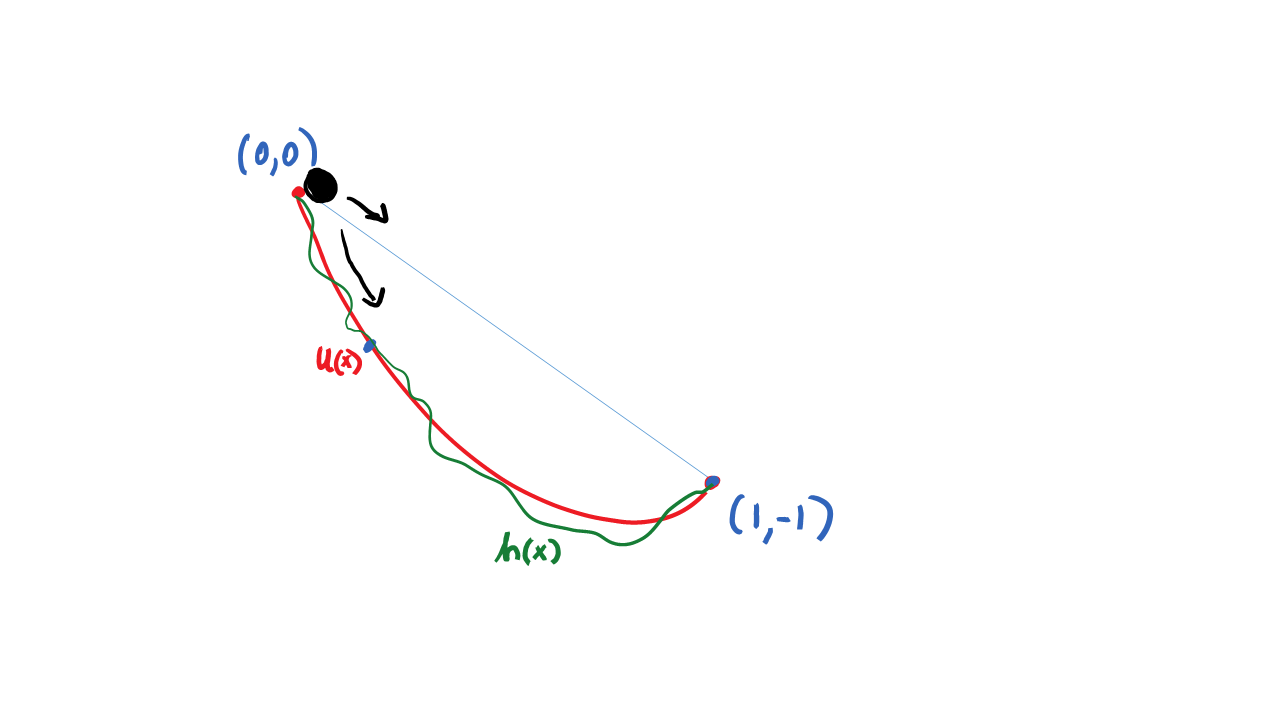
\includegraphics[width=4in]{fig3}\caption{The ``fastest'' curve\label{fig:rel-1}}
\end{figure}

\begin{proof}
Given a curve $u=u(x)$, the total travel time is
\[
T(u)=\int_{0}^{1}\frac{ds(x)}{v(x)}=\int_{0}^{1}\frac{\sqrt{1+(u'(x))^{2}}}{v(x)}dx
\]
where $ds$ is the arc length element and $v(x)$ is the velocity
at $x$. By conservation of energy, i.e., the gained kinetic energy
must equal the lost potential energy for every point along the curve,
we know that 
\[
\frac{1}{2}mv(x)^{2}=-mgu(x).
\]
Hence, we have $v(x)=\sqrt{-2gu(x)}$ and so 
\[
T(u)=\int_{0}^{1}\sqrt{\frac{1+(u'(x))^{2}}{-2gu(x)}}dx.
\]
Since $u$ is a \emph{shortest} curve, any local change in $u$ cannot
reduce the time, i.e., 
\[
DT(u)[h]=0
\]
for any change $h$ of the curve $u$. We next compute the directional
derivative of $T(u)$, i.e., $\frac{d}{dt}\vert_{t=0}T(u+th)$:
\begin{align*}
DT(u)[h] & =\int_{0}^{1}-\frac{1}{2}\frac{\sqrt{1+u'(x)^{2}}}{\sqrt{-2g}u(x)^{3/2}}\frac{d}{dt}u(x)dx+\int_{0}^{1}\frac{1}{2}\frac{2u'(x)}{\sqrt{-2gu(x)}\sqrt{1+u'(x)^{2}}}\frac{d}{dt}u'(x)dx.\\
 & =\int_{0}^{1}-\frac{1}{2}\frac{\sqrt{1+u'(x)^{2}}}{\sqrt{-2gu(x)}u(x)}h(x)dx+\int_{0}^{1}\frac{u'(x)h'(x)}{\sqrt{-2gu(x)}\sqrt{1+u'(x)^{2}}}dx.
\end{align*}
Note that the second term involves $h'(x)$. To change the term $h'(x)$
to $h(x)$, we use the integration by parts (with respect to $x$,
not $t$!):
\[
\int_{0}^{1}\frac{u'(x)h'(x)}{\sqrt{-2gu(x)}\sqrt{1+(u'(x))^{2}}}dx=\left[\frac{u'(x)h(x)}{\sqrt{-2gu(x)}\sqrt{1+(u'(x))^{2}}}\right]_{0}^{1}-\int_{0}^{1}\frac{d}{dx}\left(\frac{u'(x)}{\sqrt{-2gu(x)}\sqrt{1+(u'(x))^{2}}}\right)h(x)dx.
\]
Since the endpoints of the curve are fixed, we have $h(1)=h(0)=0$.
Hence, the first term on the right hand side is $0$. Continuing,
\begin{align*}
DT(u)[h]= & \int_{0}^{1}-\frac{1}{2}\frac{\sqrt{1+u'(x)^{2}}}{\sqrt{-2gu(x)}u(x)}h(x)dx-\int_{0}^{1}\frac{d}{dx}\left(\frac{u'(x)}{\sqrt{-2gu(x)}\sqrt{1+u'(x)^{2}}}\right)h(x)dx\\
= & \int_{0}^{1}-\frac{1}{2}\frac{\sqrt{1+(u'(x))^{2}}}{\sqrt{-2gu(x)}u(x)}h(x)dx-\int_{0}^{1}\frac{u''(x)}{\sqrt{-2gu(x)}\sqrt{1+u'(x)^{2}}}h(x)dx\\
 & +\int_{0}^{1}\frac{1}{2}\frac{u'(x)^{2}}{\sqrt{-2gu(x)}u(x)\sqrt{1+u'(x)^{2}}}h(x)dx\\
 & +\int_{0}^{1}\frac{u'(x)u'(x)u''(x)}{\sqrt{-2gu(x)}(1+u'(x){}^{2})^{3/2}}h(x)dx.
\end{align*}
Hence, we have $DT(u)[h]=\int_{0}^{1}a(x)h(x)dx$ where
\begin{align}
a(x)= & \frac{-1}{2}\frac{\sqrt{1+(u'(x))^{2}}}{\sqrt{-2gu(x)}u(x)}-\frac{u''(x)}{\sqrt{-2gu(x)}\sqrt{1+u'(x)^{2}}}+\frac{1}{2}\frac{u'(x)^{2}}{\sqrt{-2gu(x)}u(x)\sqrt{1+u'(x)^{2}}}\nonumber \\
 & +\frac{u'(x)u'(x)u''(x)}{\sqrt{-2gu(x)}(1+u'(x){}^{2})^{3/2}}.\label{brach_d}
\end{align}
Note that $a(x)$ is the gradient of $T$. Since $DT(u)[h]=0$ for
all $h(x)$, we have that $a(x)=0$ for all $x$. Multiplying both
sides of (\ref{brach_d}) by $2\sqrt{-2gu(x)}(1+(u'(x))^{2})^{3/2}u(x)$,
we have
\begin{align*}
0= & -(1+(u'(x))^{2})^{2}-2u(x)u''(x)(1+(u'(x))^{2})+u'(x)^{2}(1+(u'(x))^{2})+2u(x)u'(x)^{2}u''(x)\\
= & -1-u'(x)^{2}-2u(x)u''(x).
\end{align*}
\end{proof}

\subsection{Taking derivatives on both sides}

Suppose we have a function $f(x,y)$ and $g(x)$ such that $f(x,g(x))=0$.
The implicit function theorem shows that
\[
D_{x}f(x,g(x))+D_{y}f(x,g(x))Dg(x)=0
\]
where $D_{x}f$ is the Jacobian of $f$ with respect to $x$ variables
and $Dg(x)$ is the Jacobian of $g$. We note that the formula can
be obtained from taking derivative on both sides with respective to
$x$. Sometimes, taking derivatives on the both sides can greatly
simplify calculations. Here are some examples.
\begin{lem}
Consider $x_{t}=\argmin_{x\in\Rn}f_{t}(x)$ where $f_{t}$ are strictly
convex. Then, we have
\[
\frac{dx_{t}}{dt}=(\nabla^{2}f_{t}(x_{t}))^{-1}\nabla\frac{df_{t}}{dt}(x_{t}).
\]
\end{lem}

\begin{proof}
By the optimality condition, we have $\nabla f_{t}(x_{t})=0$. Taking
derivatives on both sides, we have
\[
\nabla^{2}f_{t}(x_{t})\frac{dx_{t}}{dt}+\nabla\frac{df_{t}}{dt}(x_{t})=0.
\]
Since $f_{t}$ are strictly convex, $\nabla^{2}f_{t}(x_{t})$ is positive
definite and is invertible. Hence, we have that the result.
\end{proof}
In section \ref{sec:IPM}, we used this to compute the derivative
of central path.

\subsection{Linearity of Expectation - the continuous version}

Often times one would like to compute the differential of a quantity
that is most appropriately expressed by an integral, and under mild
assumptions we can do so by simply swapping the integral and derivative,
i.e. for time differentiable and (Lebesgue) integrable $f(x,t)$ we
want to do
\[
\frac{d}{dt}\int_{\Omega}f(x,t)dx=\int_{\Omega}\frac{\partial}{\partial t}f(x,t)dx
\]
For example, we use this trick in deriving the Fokker-Planck equation
in gradient-based sampling. Fortunately, measure theory gives us the
dominated convergence theorem, a quick corollary of which tells us
we can perform the above trick as long as there exists integrable
$g:\Omega\rightarrow\R$ such that $\big|\frac{\partial}{\partial t}f(x,t)\big|\leq g(x)$
for all $x$. If we have $\Omega=\Rn$, then similar in nature to
integration by parts for divergence, the upper bound follows from
showing that the derivative of $f$ decays fast enough at infinity
(for absolutely continuous probability distributions with full support,
this is often the case).

\section{Solving optimization problems by hand}

In this section, we introduce the KKT condition and show how to use
it to solve optimization problem by hand.
\begin{thm}[Karush--Kuhn--Tucker theorem]
Consider the following optimization problem
\[
\min_{x\in\Omega}f(x)\text{ subject to }h_{i}(x)\leq0\text{ and }\ell_{j}(x)=0\text{ for all }i,j
\]
for some open set $\Omega$ and continuously differentiable functions
$f$, $h_{i}$ and $\ell_{j}$. If $x$ is a local minimum, $x$ satisfies
the KKT conditions:
\begin{itemize}
\item Stationary: $\nabla f(x)+\sum_{i}u_{i}\nabla h_{i}(x)+\sum_{j}v_{j}\nabla\ell_{j}(x)=0$
\item Complementary Slackness: $u_{i}h_{i}(x)=0$ for all $i$
\item Primal Feasibility: $h_{i}(x)\leq0$ and $\ell_{j}(x)=0$ for all
$i,j$
\item Dual Feasibility: $u_{i}\geq0$ for all $i$
\end{itemize}
We prove Holder's inequality as an example:
\end{thm}

\begin{fact}
For any vector $x,y\in\R^{n}$, we have $\|xy\|_{1}\leq\|x\|_{p}\|y\|_{q}$
for any $1\leq p\leq\infty$ and $1\leq q\leq\infty$ with $\frac{1}{p}+\frac{1}{q}=1$.
\end{fact}

\begin{proof}
By symmetries, it suffices to compute
\[
\max_{\|x\|_{p}\leq1}\sum_{i}x_{i}y_{i}
\]
for non-zero $y$. Now, we use the KKT theorem with $f(x)=-\sum_{i}x_{i}y_{i}$,
$h(x)=\|x\|_{p}-1$ and $\Omega=\R^{n}$. By the KKT conditions, for
any maximizer $x$, we have that
\begin{align*}
-\nabla f(x)+u\nabla h(x) & =0,\\
uh(x) & =0,\\
h(x)\leq0, & u\geq0.
\end{align*}
Note that $\nabla f(x)=y$ and $(\nabla h(x))_{i}=\frac{1}{p}\|x\|_{p}^{1-p}\cdot px_{i}^{p-1}=\|x\|_{p}^{1-p}\cdot x^{p-1}$.
From the stationary condition, we have
\[
y=u\|x\|_{p}^{1-p}\cdot x^{p-1}.
\]

To compute $u$, we note that $y$ is non-zero and hence $u\neq0$.
From the complementary slackness, we have $h(x)=0$ and hence $\|x\|_{p}=1$.
Therefore, we have
\[
y=u\cdot x^{p-1}.
\]
Hence, we have $1=\sum_{i}x_{i}^{p}=\sum_{i}(y_{i}/u)^{\frac{p}{p-1}}=\sum_{i}(y_{i}/u)^{q}$.
Hence, we have $u=\|y\|_{q}$ 

Now, we can compute $\sum_{i}x_{i}y_{i}$ as follows
\[
\sum_{i}x_{i}y_{i}=\sum_{i}(\frac{y_{i}}{u})^{\frac{1}{p-1}}y_{i}=\frac{1}{u^{1/(p-1)}}\sum_{i}y_{i}^{p/(p-1)}=\|y\|_{q}.
\]
\end{proof}



\chapter{Notation }

\begin{center}
\begin{tabular}{|c|c|}
\hline 
Symbol & Description\tabularnewline
\hline 
\hline 
$o_{\epsilon}(f)$ & $o(f)$ for any fixed $\epsilon$\tabularnewline
\hline 
$\langle a,b\rangle$ & Inner product $a^{T}b$\tabularnewline
\hline 
nnz & Number of nonzeros\tabularnewline
\hline 
$\tilde{O}(\cdot)$ & Asymptotic complexity ignoring logarithmic terms\tabularnewline
\hline 
$O^{*}(\cdot)$ & Asymptotic complexity ignoring logarithmic terms and error terms\tabularnewline
\hline 
$B^{n}$ & Unit Euclidean ball in $\R^{n}$\tabularnewline
\hline 
$B_{p}(x,r)$ & $p$-norm ball of radius $r$ centered at $x$\tabularnewline
\hline 
$\norm{\cdot}_{p}$ & $p$-norm: $\left(\sum_{i}\left|x_{i}\right|^{p}\right)^{1/p}$ \tabularnewline
\hline 
\end{tabular}
\par\end{center}
\end{document}

\chapter{----}

\chapter{Expansion}

\selectlanguage{american}%

\section{Ordinary Differential Equations}

We consider the first-order ODE 
\begin{align*}
\frac{\d}{\d t}x(t)= & ~F(x(t),t),\quad\forall0\leq t\leq T,\\
x(0)= & ~v.
\end{align*}
where $F:\R^{d+1}\rightarrow\R$. The basic idea to solve it comes
from the Picard-Lindel�f theorem, a constructive existence proof for
a large class of ODEs.

\subsection{Picard-Lindel�f theorem}

\label{sec:picard_lindelof} In general, we can rewrite the first-order
ODE as an integral equation 
\[
x(t)=v+\int_{0}^{t}F(x(s),s)\d s\quad\text{for all }0\leq t\leq T.
\]

To simplify the notation, we use $\mathcal{C}([0,T],\R^{d})$ to denote
$\R^{d}$-valued functions on $[0,T]$. We define the operator $\T$
from $\mathcal{C}([0,T],\R^{d})$ to $\mathcal{C}([0,T],\R^{d})$
by 
\begin{equation}
\T(x)(t)=v+\int_{0}^{t}F(x(s),s)\d s\quad\text{for all }0\leq t\leq T.\label{eq:def_T_operator}
\end{equation}
Therefore, the integral equation is simply $x=\T(x)$. Let $\T^{\circ j}$
be the composition of $j$ many $\T$, i.e., 
\begin{align*}
\T^{\circ j}(x)=\underbrace{\T(\T(\cdots\T}_{j~\text{many}~\T}(x)\cdots)).
\end{align*}

The Banach fixed point theorem says that the integral equation $x=\T(x)$
has a unique solution if there is a norm, and $j\in\mathbb{N}$ such
that the map $\T^{\circ j}$ has Lipschitz constant less than 1.

The Picard-Lindel�f theorem shows that if $F$ is Lipschitz in $x$,
then the map $\T^{\circ j}$ has Lipschitz constant less than 1 for
some positive integer $j$.
\begin{thm}
\label{lem:Lipschitz_T} Given any norm $\|\cdot\|$ on $\R^{d}$.
Let $L$ be the Lipschitz constant of $F$ in $x$, i.e. 
\[
\|F(x,s)-F(y,s)\|\leq L\|x-y\|\quad\text{for all }x,y\in\R^{d},s\in[0,T].
\]
For any $x\in\mathcal{C}([0,T],\R^{d})$, we define the corresponding
norm 
\[
\|x\|\defeq\max_{0\leq t\leq T}\|x(t)\|.
\]
Then, the Lipschitz constant of $\T^{\circ j}$ in this norm is upper
bounded by $(LT)^{j}/j!$.
\end{thm}

\begin{proof}
We prove this lemma with a stronger induction hypothesis
\[
\|(\T^{\circ j}x)(h)-(\T^{\circ j}y)(h)\|\leq\frac{L^{j}h^{j}}{j!}\|x-y\|\quad\text{for all }0\leq h\leq T.
\]
The base case $j=0$ is trivial. For the inductive step, 
\begin{align*}
~\|\T^{\circ j}x(h)-\T^{\circ j}y(h)\|= & ~\|\T\T^{\circ(j-1)}x(h)-\T\T^{\circ(j-1)}y(h)\|\\
%=\leq
\end{align*}
This completes the proof.
\end{proof}
To make the Picard-Lindel�f theorem algorithmic, we have to decide
how to represent a function in $\mathcal{C}([0,T],\R^{d})$. One standard
way is to use a polynomial $p_{i}(t)$ in $t$ for each coordinate
$i\in[d]$. More generally, suppose there is a basis $\{\varphi_{j}\}_{j=1}^{D}\subset\mathcal{C}([0,T],\R)$
such that for all $i\in[d]$, $\frac{\d x_{i}}{\d t}$ is approximated
by some linear combination of $\varphi_{j}(t)$. For example, if $\varphi_{j}(t)=t^{j-1}$
for $j\in[D]$, then our assumption is simply saying $\frac{\d x_{i}}{\d t}$
is approximated by a degree $D-1$ polynomial. Other possible basis
are piecewise-polynomial and Fourier series. By Gram-Schmidt orthogonalization,
we can always pick points $\{c_{i}\}_{j=1}^{D}$ such that 
\[
\varphi_{j}(c_{i})=\delta_{i,j}\quad\text{for }i,j\in[D].
\]
The benefit of such a basis is that for any $f\in\text{span}(\varphi_{j})$,
we have that $f(t)=\sum_{j=1}^{D}f(c_{j})\varphi_{j}(t).$

For polynomials, we can use the basis consisting of the Lagrange polynomials:
\[
\varphi_{j}(t)=\prod_{i\in[D]\backslash\{j\}}\frac{t-c_{i}}{c_{j}-c_{i}}\quad\text{for }j\in[D].
\]
The only assumption we make on the basis is that it is bounded in
the following sense.
\begin{defn}
\label{def:basis} Given a $D$ dimensional subspace $\mathcal{V}\subset\mathcal{C}([0,T],\R)$
and node points $\{c_{j}\}_{j=1}^{D}\subset[0,T]$. For any $\gamma_{\varphi}\geq1$,
we say that a basis $\{\varphi_{j}\}_{j=1}^{D}\subset\mathcal{V}$
is $\gamma_{\varphi}$-bounded if $\varphi_{j}(c_{i})=\delta_{i,j}$
and we have 
\[
\sum_{j=1}^{D}\left|\int_{0}^{t}\varphi_{j}(s)\d s\right|\leq\gamma_{\varphi}T\quad\text{for }t\in[0,T].
\]
\end{defn}

Note that if the constant function $1\in\mathcal{V}$, then we have
\[
1=\sum_{j=1}^{D}1(c_{j})\varphi_{j}(t)=\sum_{j=1}^{D}\varphi_{j}(t).
\]
Hence,
\[
T=\int_{0}^{T}1\d s\leq\sum_{j=1}^{D}\left|\int_{0}^{T}\varphi_{j}(s)\d s\right|\leq\gamma_{\varphi}T.
\]
Therefore, $\gamma_{\varphi}\geq1$ for most elements. Later we will
see that for the space of low degree polynomials or piece-wise low-degree
polynomials, there is a basis on the Chebyshev nodes that is $O(1)$-bounded.

Assuming that $\frac{dx}{dt}$ can be approximated by some element
in $\mathcal{V}$, we have that 
\[
\frac{\d x}{\d t}(t)\sim\sum_{j=1}^{D}\frac{\d x}{\d t}(c_{j})\varphi_{j}(t)=\sum_{j=1}^{D}F(x(c_{j}),c_{j})\varphi_{j}(t).
\]
Integrating both sides, we have 
\begin{equation}
x(t)\approx v+\int_{0}^{t}\sum_{j=1}^{D}F(x(c_{j}),c_{j})\varphi_{j}(s)\d s.\label{eq:approx_fix_point}
\end{equation}
This suggests the following operator from $\mathcal{C}([0,T],\R^{d})$
to $\mathcal{C}([0,T],\R^{d})$: 
\begin{equation}
\mathcal{T}_{\varphi}(x)(t)_{i}=v_{i}+\int_{0}^{t}\sum_{j=1}^{D}F(x(c_{j}),c_{j})_{i}\varphi_{j}(s)\d s\quad\text{for }i\in[d].\label{eq:def_T_d_operator}
\end{equation}
Equation (\ref{eq:approx_fix_point}) can be written as $x\approx\mathcal{T}_{\varphi}(x).$
To find $x$ that satisfies this, naturally, one can apply a fix point
iteration and the resulting algorithm is called the collocation method.\selectlanguage{english}%

\input{collocation_method.tex}

\chapter{Decomposition}

\selectlanguage{american}%

\section{Cholesky Decomposition}\selectlanguage{english}%

\selectlanguage{american}%

\section{Multigrid Methods}\selectlanguage{english}%


\end{document}
